\documentclass[deutsch,oneside,color]{htldipl}
% die folgende Zeile einkommentieren für Arial-Ähnliche Schriftart
%\renewcommand{\familydefault}{\sfdefault}

\graphicspath{{images/}}    		% Bilderverzeichnis


\usepackage[paper=a4paper,margin=3cm]{geometry}

\makeindex[title=Index]
\makeindex[name=allgemein, title=Allgemeiner Index]
\makeindex[name=name,title={Autoren Index}]
\makeindex[name=title,columns=1,title={Literatur Index}]
\indexsetup{level=\subsection*, toclevel=subsection, noclearpage}


\makeatletter
\@ifpackageloaded{biblatex_legacy}
  {\DeclareIndexNameFormat{default}{%
     \usebibmacro{index:name}{\index[name]}{#1}{#3}{#5}{#7}}}
  {\DeclareIndexNameFormat{default}{%
     \usebibmacro{index:name}{\index[name]}
       {\namepartfamily}
       {\namepartgiven}
       {\namepartprefix}
       {\namepartsuffix}}}
\makeatother

\DeclareIndexFieldFormat{indextitle}{%
  \usebibmacro{index:title}{\index[title]}{#1}}

\renewbibmacro*{bibindex}{%
  \ifbibindex
    {\indexnames{author}%
     \indexnames{editor}%
     \indexnames{translator}%
     \indexnames{commentator}%
     \indexfield{indextitle}}
    {}}

\makeatletter
\DeclareCiteCommand{\repeatfootcite}[\cbx@wrap]
  {\gdef\cbx@keys{}}
  {\xappto\cbx@keys{\thefield{entrykey},}}
  {}
  {\ifcsundef{cbx@lastin@\cbx@keys @\strfield{postnote}}
     {\csnumgdef{cbx@lastin@\cbx@keys @\strfield{postnote}}{-1}}{}%
   \ifsamepage{\value{instcount}}{\csuse{cbx@lastin@\cbx@keys @\strfield{postnote}}}
     {\footnotemark[\csuse{cbx@lastfn@\cbx@keys @\strfield{postnote}}]}
     {\xappto\cbx@cite{\noexpand\footcite%
        [\thefield{prenote}][\thefield{postnote}]{\cbx@keys}%
        \csnumgdef{cbx@lastfn@\cbx@keys @\strfield{postnote}}{\value{\@mpfn}}%
        \csnumgdef{cbx@lastin@\cbx@keys @\strfield{postnote}}{\value{instcount}}}}}

\newrobustcmd{\cbx@wrap}[1]{#1\cbx@cite\gdef\cbx@cite{}}
\def\cbx@cite{}
\makeatother



\makeglossaries
\loadglsentries{glossary}		   	% beinhaltet Daten für das Glossar
\addbibresource{literatur.bib}     	% beinhaltet Daten für das Literarturverzeichnis

%%%----------------------------------------------------------
\begin{document}

	
\newcommand{\fib}{\marginpar{\scriptsize{\textit{$\rightarrow$Fischbacher}}}}
\newcommand{\pra}{\marginpar{\scriptsize{\textit{$\rightarrow$Prinz}}}}
\newcommand{\hon}{\marginpar{\scriptsize{\textit{$\rightarrow$Homolka}}}}
\newcommand{\prc}{\marginpar{\scriptsize{\textit{$\rightarrow$Passet}}}}
%%%----------------------------------------------------------
\title{Entity Relationship Modelling Toolkit ERD}
\abteilung{Informatik}
\schwerpunkt{}
\studienort{Wiener Neustadt}
\schule{HTBLuVA Wiener Neustadt}
\schullogo{htl.jpeg}
\abgabejahr{2018/19}

\betreuerA{Dipl.-Ing. Günther Burgstaller}
\betreuerB{}
\betreuerC{}
\betreuerD{}
\betreuerD{}

\schuelerA{Berndt FISCHBACHER}
\evidenzA{5BHIF}
\subthemaA{}
\schuelerB{Christian PASSET}
\evidenzB{5BHIF}
\subthemaB{}
\schuelerC{Andreas PRINZ}
\evidenzC{5BHIF}
\subthemaC{}
\schuelerD{Nicolas HOMOLKA}
\evidenzD{5BHIF}
\subthemaD{}
\schuelerE{}
\evidenzE{}
\subthemaE{}
\schuelerE{}
\evidenzE{}
\subthemaE{}

%%%----------------------------------------------------------
\frontmatter
\maketitle
\tableofcontents
%%%----------------------------------------------------------

\chapter{Vorwort}

Dies ist \textbf{Version \htldiplDate} der \latex-Dokumentenvorlage für 
die Diplomarbeiten an der HTL Wiener Neustadt, basierend auf der
Vorlage für Abschlussarbeiten an der FH Hagenberg erstellt von Dr.\ Wilhelm
Burger\footnote{\url{http://www.fh-hagenberg.at/staff/burger/diplomarbeit/}}.

Die Verwendung dieser Vorlage ist jedermann freigestellt und an
keinerlei Erwähnung gebunden. Allerdings -- wer sie als Grundlage
seiner eigenen Arbeit verwenden möchte, sollte nicht einfach
("`ung'schaut"') darauf los werken, sondern zumindest die
wichtigsten Teile des Dokuments \emph{lesen} und nach Möglichkeit
auch beherzigen. Die Erfahrung zeigt, dass dies die Qualität der
Ergebnisse deutlich zu steigern vermag.

Der Quelltext zu diesem Dokument sowie das zugehörige
\latex-Paket sind in der jeweils aktuellen Version online
verfügbar unter
%
\begin{quote}
\url{https://github.com/wschermann/Diplomarbeitsvorlage}
\end{quote}
%
Trotz großer Mühe enthält dieses Dokument zweifellos Fehler und Unzulänglichkeiten
-- Kommentare, Verbesserungsvorschläge und passende Ergänzungen
sind daher stets willkommen, am einfachsten per E-Mail direkt an mich:
\begin{center}%
\begin{tabular}{l}
\nolinkurl{w.schermann@htlwrn.ac.at} \\
Wolfgang Schermann MSc \\
HTL Wiener Neustadt -- Informatik\\
Austria
\end{tabular}
\end{center}

\noindent
Übrigens, hier im Vorwort kann man kurz auf die Entstehung  des Dokuments eingehen.
Hier ist auch der Platz für allfällige Danksagungen (\zB an den Betreuer, 
den Begutachter, die Familie, den Hund, ...), Widmungen und philosophische 
Anmerkungen. Das sollte man allerdings auch nicht übertreiben und sich auf 
einen Umfang von maximal zwei Seiten beschränken.




				%ggfs. weglassen
%Inkludiert die 4. vorgeschriebenen Seiten an Dokumentation aus dem gedruckten PDF-Formular
%Das Formular erst vor der Abgabe vollständig ausfüllen, da z.B. das Bild zur Diplomarbeit vorher nicht vorhanden sein wird
\begingroup
\makeatletter
\newpage
\@twosidefalse
\includepdf[pages=1-1,pagecommand={\chapter[Diplomarbeit Dokumentation]{}}]{pdf/Formular-printed.pdf}
\includepdf[pages=2-2,pagecommand={\thispagestyle{plain}}]{pdf/Formular-printed.pdf}
\includepdf[pages=3-3,pagecommand={\chapter[Diploma Thesis Documentation]{}}]{pdf/Formular-printed.pdf}
\includepdf[pages=4-4,pagecommand={\thispagestyle{plain}}]{pdf/Formular-printed.pdf}
\endgroup
\part{Kurzfassung}

\chapter{Kurzfassung}
\label{cha:Kurzfassung }

\noindent
In der Diplomarbeit ERMTK-ERD wurde ein Programm entwickelt, das dazu dient automatisch Entity-Relationship Diagramme aus XML-Dateien zu generieren
Diese Generierung wurde mit vier verschiedenen Ausgabeformaten implementiert. Um diese vier Variationen zu einem Tool zu kombinieren wurde die Diplomarbeit Entity-Relationship-Modeling-Toolkit ins Leben gerufen. Außerdem soll durch Angabe von Kommandozeilenparameter das Aussehen der Diagramme durch den Benutzer verändert werden können. Die vier verschiedenen Ausgabeformate sind:
\begin{itemize}
	\item Graphml
	\item LibreOffice Draw
	\item PIC-Code
	\item Graphviz
\end{itemize}   		
\chapter{Abstract}

\begin{english} %switch to English language rules
This should be a 1-page (maximum) summary of your work in English.
%und hier geht dann das Abstract weiter...
\end{english}

Im englischen Abstract sollte inhaltlich das Gleiche
stehen wie in der deutschen Kurzfassung. Versuchen Sie daher, die
Kurzfassung prä\-zise umzusetzen, ohne aber dabei Wort für Wort zu
übersetzen. Beachten Sie bei der Übersetzung, dass gewisse
Redewendungen aus dem Deutschen im Englischen kein Pendant haben
oder völlig anders formuliert werden müssen und dass die
Satzstellung im Englischen sich (bekanntlich) vom Deutschen stark
unterscheidet (mehr dazu in Abschn.\ \ref{sec:englisch}). Es
empfiehlt sich übrigens -- auch bei höchstem Vertrauen in die
persönlichen Englischkenntnisse -- eine kundige Person für das
"`proof reading"' zu engagieren.

Die richtige Übersetzung für "`Diplomarbeit"' ist übrigens
schlicht \emph{thesis}, allenfalls  "`diploma thesis"', auf keinen Fall aber "`diploma work"' oder gar "`dissertation"'. 

Übrigens sollte für diesen Abschnitt die \emph{Spracheinstellung} in \latex\ von Deutsch
auf Englisch umgeschaltet werden, um die richtige Form der
Silbentrennung zu erhalten, die richtigen Anführungszeichen muss
man allerdings selbst setzen %
(s.\ dazu Abschnitt \ref{sec:sprachumschaltung} %
bzw.\ \ref{sec:anfuehrungszeichen}).
			

%%%----------------------------------------------------------
\mainmatter           %Hauptteil (ab hier arab. Seitenzahlen)
%%%----------------------------------------------------------

\chapter{Einleitung}
\label{cha:Einleitung}

\section{Zielsetzung}
Dieses Dokument ist als vorwiegend technische Starthilfe für das
Erstellen einer Diplomarbeit mit \latex
gedacht und ist die Weiterentwicklung einer früheren
Vorlage\footnote{Nicht mehr verfügbar.} für das Arbeiten mit
Microsoft \emph{Word}. Während ursprünglich daran gedacht war, die
bestehende Vorlage einfach in \latex zu übernehmen, wurde rasch
klar, dass allein aufgrund der großen Unterschiede zum Arbeiten
mit \emph{Word} ein gänzlich anderer Ansatz notwendig wurde. Dazu
kamen zahlreiche Erfahrungen mit Diplomarbeiten in den
nachfolgenden Jahren, die zu einigen zusätzlichen Hinweisen Anlass gaben.

Das vorliegende Dokument dient einem zweifachen Zweck: 
\emph{erstens} als Erläuterung und Anleitung, \emph{zweitens} als
direkter Ausgangspunkt für die eigene Arbeit. Angenommen wird,
dass der Leser bereits über elementare Kenntnisse im Umgang mit
\latex verfügt. In diesem Fall sollte -- eine einwandfreie
Installation der Software vorausgesetzt -- der Arbeit nichts mehr
im Wege stehen. Auch sonst ist der Start mit \latex\ nicht
schwierig, da viele hilfreiche Informationen auf den zugehörigen
Webseiten zu finden sind (s.\ Abschn.~\ref{sec:latex}).





\section{Warum {\latex}?}

Diplomarbeiten, Dissertationen und Bücher im
technisch-natur\-wissen\-schaft\-lichen Bereich werden
traditionell mithilfe des Textverarbeitungssystems \latex
\footcite{Lamport94,Lamport95} gesetzt. Das hat gute Gründe, denn
\latex ist bzgl.\ der Qualität des Druckbilds, des Umgangs mit
mathematischen Elementen, Literaturverzeichnissen etc.\
unübertroffen und ist noch dazu frei verfügbar. Wer mit \latex
bereits vertraut ist, sollte es auch für die Diplomarbeit
unbedingt in Betracht ziehen, aber auch für den Anfänger sollte
sich die zusätzliche Mühe am Ende durchaus lohnen.

Für den professionellen elektronischen Buchsatz wurde bisher
häufig \emph{Adobe Framemaker} verwendet, allerdings ist diese
Software teuer und komplex. Eine modernere Alternative dazu ist
\emph{Adobe InDesign}, wobei allerdings die Erstellung
mathematischer Elemente und die Verwaltung von Literaturverweisen
zur Zeit nur rudimentär unterstützt werden.%
\footnote{Angeblich werden aber für den (sehr sauberen) Schriftsatz 
in \emph{InDesign} ähnliche Algorithmen wie in \latex\ verwendet.}

Microsoft \emph{Word} gilt im Unterschied zu \latex, 
\emph{Framemaker} und \emph{InDesign} übrigens nicht als professionelle
Textverarbeitungssoftware, obwohl es immer häufiger auch von
großen Verlagen verwendet wird.%
\footnote{Siehe auch \url{http://latex.tugraz.at/mythen.php}.}
Das Schriftbild in \emph{Word}
lässt -- zumindest für das geschulte Auge -- einiges zu wünschen
übrig und das Erstellen von Büchern und ähnlich großen Dokumenten
wird nur unzureichend unterstützt. Allerdings ist \emph{Word} sehr
verbreitet, flexibel und vielen Benutzern zumindest oberflächlich
vertraut, sodass das Erlernen eines speziellen Werkzeugs wie
\latex\ ausschließlich für das Erstellen einer Diplomarbeit
manchen verständlicherweise zu mühevoll ist. Man sollte es daher
niemandem übel nehmen, wenn er/sie sich auch bei der Diplomarbeit
auf \emph{Word} verlässt. Im Endeffekt lässt sich mit etwas
Sorgfalt (und ein paar Tricks) auch damit ein durchaus akzeptables
Ergebnis erzielen. Für alle, die so denken, finden sich in
Kap.~\ref{chap:Word} einige spezielle Hinweise zum Arbeiten mit
\emph{Word}. Ansonsten sollten für \emph{Word}-Benutzer aber auch
andere Teile dieses Dokuments von Interesse sein, insbesondere die
Abschnitte über Abbildungen und Tabellen
(Kap.~\ref{chap:Abbildungen}) und mathematische Elemente
(Kap.~\ref{chap:Mathematik}).






Übrigens, genau hier am Ende des Einleitungskapitels (und nicht
etwa in der Kurzfassung) ist der richtige Platz, um die
inhaltliche Gliederung der nachfolgenden Arbeit zu beschreiben.
Hier soll dargestellt werden, welche Teile (Kapitel) der Arbeit
welche Funktion haben und wie sie inhaltlich zusammenhängen. Auch
die Inhalte des \emph{Anhangs} -- sofern vorgesehen -- sollten hier
kurz beschrieben werden.





\newcommand{\subsubsubsection}[1]{\paragraph{#1}\mbox{}\\}
\setcounter{secnumdepth}{4}
\setcounter{tocdepth}{4}




\part{Methodik}

\chapter{Methoden}
\label{cha:Einleitung}



\noindent
\section{Python}
\fib{}
\subsection{Entwicklung}

\noindent
Die im Jahre 1991 von Guido van Rossum, einem niederländischen Software-Entwickler, veröffentlichte Programmiersprache Python wurde ursprünglich für das Betriebssystem Amoeba entwickelt und sollte die Programmier-Lehrsprache ABC ablösen.
Mit der ersten Vollversion, die unter dem Namen Python 1.0 im Jahre 1994 erschienen ist, wurden einige Konzepte der funktionalen Programmierung implementiert, jedoch wurden diese später wieder aufgegeben. 
Im Jahre 2000 erschien Python 2.0 mit einer voll funktionsfähigen Garbage Collection, sowie die Unterstützung für den Unicode-Zeichensatz.
Python 3.0 wurde 8 Jahre später am 3.Dezember 2008 veröffentlicht. Mit der Version 3.0 kamen tiefgreifende Änderungen an der Sprache, die dazu führten, dass sich die Python Software Foundation dafür entschied, Python 2.7 und Python 3.0 bis Ende 2019 parallel mit neuen Versionen zu unterstützen. 
Die neuste Version ist Version 3.7, die am 27.Juni 2018 erschienen ist.
\footcite{noauthor_history_nodate}

\subsection{Idee und Zweck}

\noindent
Python ist eine sehr übersichtliche und einfache Programmiersprache und war in erster Linie dafür gedacht, das Programmieren zu erlernen. Das wird erzielt, in dem Python mit wenigen Schlüsselwörtern auskommt und die Syntax, im Vergleich zu anderen Programmiersprachen, sehr reduziert ist. Außerdem ist die Standardbibliothek von Python überschaubar und leicht erweiterbar, was zu folge hatte, dass heute eine Vielzahl an Bibliotheken zu Verfügung stehen. 
\footcite{noauthor_general_nodate}

\subsection{Verwendung}

\noindent
Da Python über eine große Vielfalt an Bibliotheken verfügt, einfach zu programmieren ist und der Code leicht zu lesen ist, bot es sich für dieses Projekt hervorragend an. Beispielsweise für die Implementierung der Umsetzung mittels Graphviz, die durch die von Graphviz zu Verfügung gestellten Bibliothek mit dem gleichen Namen programmiert wurde.
Ein anderes Beispiel wo dieses Projekt von Python profitiert hat, ist die Eigenschaft von Python, dass es möglich ist, Python-Programme als Module in anderen Sprachen einzubetten.
\footcite{noauthor_integrateddevelopmentenvironments_nodate}

\section{Pycharm als IDE}
\fib{}
\subsection{Allgemeines}

\subsubsection{Version}

\noindent
PyCharm ist eine IDE vom Unternehmen JetBrains, die im Juli 2010 erschienen ist und viele Eigenschaften sowie Features mit den anderen IDEs von JetBrains teilt. Dabei hat JetBrains wie der Name PyCharm schon andeutet, die IDE explizit für die Programmiersprache Python entwickelt. Die aktuellste Version ist die Version 2018.3.5, die am 27. Februar 2019 erschienen ist. Jedoch ist die neue Version 2019.1 schon in Entwicklung und wird noch im zweiten Quartal von 2019 verfügbar sein. 
In der Regel werden jedes Jahr ca. drei neue Versionen veröffentlicht, jedoch handelt es sich dabei eher um kleinere Updates oder Hotfixes und nicht um große Erneuerungen.
\footcite{noauthor_pycharm:_nodate}

\subsubsection{Editionen}

\noindent
Außerdem gibt es PyCharm in drei verschiedenen Varianten, einmal die PyCharm Community Edition, die PyCharm Professional Edition und die PyCharm Educational Edition.
\footcite{noauthor_previous_nodate}

\noindent
\begin{itemize}
    \item Die Community Edition ist Open-Source und damit gratis für jeden erhältlich. 
    \item Die Professional Edition verfügt über mehr Features, man benötigt für diese Version jedoch eine Lizenz die man kaufen muss.Für dieses Projekt wurde die Professional Edition verwendet, da JetBrains die Lizenzen gratis für Schulen anbietet.
    \item Die dritte Edition ist zum Erlernen von Python gedacht.
\end{itemize}



\subsection{Funktionen}
\subsubsection{Intelligenter Code Editor}

\noindent
PyCharm bietet intelligente Code Vervollständigung, Syntax Hervorhebung, automatische Code Refactorings.
Die IDE erkennt wenn Code-Teile kopiert wurden und macht dem entsprechen Vorschläge für das Refactoring.
\footcite{noauthor_features_nodate}

\subsubsection{Web Development Frameworks}

\noindent
PyCharm unterstützt auch spezifische Web Development Frameworks wie z.B.:

\begin{itemize}
    \item Django
    \item Flask
    \item Google App Engine
    \item web2py
\end{itemize}

\subsubsection{Cross-technology Development}

\noindent
Neben Python unterstützt die IDE auch noch andere Sprachen wie z.B.: JavaScript, TypeScript, SQL und HTML/CSS.

\subsubsection{Built-in Developer Tools}

\noindent
Debuggen, Testen und Profiling ist mit PyCharm durch eine Vielzahl an GUI Elementen einfach und schnell möglich. Automatisches Einsätzen auf einem entfernten Rechner kann einfach eingestellt werden und außerdem bietet die IDE eine schnelle und benutzerfreundliche GUI für Versionsverwaltungsprotokolle wie z.B.: Git, Mercurial und SVN.

\subsection{Vorteile}
\fib{}
\noindent
\begin{itemize}
\item Ein Vorteilen der IDE ist der Support der mittels Forum oder Mail Kontakt direkt mit den Entwicklern erfolgt.
\item Neben dem Support wird bei JetBrains auch die Benutzerfreundlichkeit ihrer IDE. Die einzelnen Funktionen sind übersichtlich von den anderen getrennt und in den Untermenü mit gut erkennbaren Symbolen gekennzeichnet.
\item Der WSL Interpreter war bei dem Projekt eine große Hilfe, da nicht jeder auf dem selben Betriebssystem arbeitete. Dadurch konnte man selbst, wenn auf einem Rechner mit Windows gearbeitet wurde, in einer Linux Umgebung testen.
\item Durch die große Community von PyCharm und JetBrains gibt es für jede IDE eine Vielzahl an Plugins, die nicht nur das Programmieren vereinfachen, sondern auch die Versionsverwaltung.
\item Durch die REPL Python Konsole wird dem Entwickler das Testen vereinfacht, da man direkt von der IDE aus das Programm starten, testen und Fehlerbehebung kann. Außerdem wird einem der derzeitige Zustand der Variablen angezeigt.
\end{itemize}
\footcite{noauthor_features_nodate}

\newpage
\section{XML}

\subsection{Allgemeines zu XML}
\pra
\subsubsection{Definition}
\noindent
Das Datenformat \textit{Extensible Markup Language (XML)} ist mittlerweile weit verbreitet und dient häufig als Basis für viele Technologien. XML wird im Buch ,,\citetitle[][]{taschenbuch}''\footfullcite{taschenbuch} wie folgt definiert:

\begin{quote}
	XML wurde mit der Zielsetzung des erleichterten Datenaustausches als Vereinfachung seines Vorgängerstandards \textit{SGML} eingeführt. Inzwischen ist es aber viel mehr als das: Es bildet beispielsweise die Grundlage vieler Technologien der serviceorientierten Architektur. XML wird dabei zur Definition von Sprachen verwendet und legt gleichzeitig die Basissyntax für diese Sprachen fest.  
\end{quote}


\subsubsection{Aufbau einer XML Datei}
\pra
Der Aufbau einer \textit{XML}-Datei ist mit \textit{XML-Elementen} versehen. Die einzelnen \textit{XML-Elemente} sind selbst wählbar. Die Daten werden innerhalb dieser \textit{Elemente} gespeichert. \footfullcite{ausarbeitung_xml}
\\

\noindent
In einem \textit{XML-Document} befindet sich der Code der eigentlichen Daten, jedoch kann auch eine \textit{XML-Deklaratio} angegeben werden. Diese ist jedoch optional. In dieser \textit{Deklaration} befinden sich Informationen zu der Version des Datenformats sowie über die \textit{XML-Attribute} \textit{encoding} und \textit{standalone}. \footnotemark[9]

\begin{verbatim} 
<?xml version="1.0" encoding="UTF-8" standalone="no"?>
\end{verbatim}

\noindent
\begin{itemize}
	\item{\textit{version}} gibt die aktuelle Version an, welche in dem Dokument verwendet wird. Standardmäßig beträgt dieser Wert \verb|1.0|.
	\item{\textit{encoding}} gibt an, welche Kodierung der Zeichen benutzt werden soll. Standardmäßig gilt \textit{UTF-8} als verwendete Kodierung.
	\item{\textit{standalone}} gibt an, ob auf eine externe \textit{Document-Type-Definition} zugegriffen werden muss, um korrekte Werte für bestimmte Teile zu ermitteln. Der Standardwert für dieses \textit{XML-Attribut} ist mit \textit{no} definiert.\footnotemark[9]
\end{itemize}

\noindent
Sowohl \textit{encoding} als auch \textit{standalone} stellen optionale\textit{XML-Attribute} dar. Falls diese nicht explizit angegeben werden, gelten die zuvor erwähnten Standardausprägungen.\footnotemark[9]
\\

\noindent
Im restlichen Dokument können dann beliebig viele \textit{XML-Elemente} erstellt werden. Jedoch gilt zu beachten, dass \textit{XML} eine gewisse Syntax verlangt. Unter anderem muss jeder Datensatz über einen Start-Tag und einen End-Tag verfügen.\footnotemark[9]

\begin{verbatim}
<Autor>
    <name> Andreas Prinz </name>
</Autor>
\end{verbatim}

\noindent
Bei der Namensgebung der \textit{XML-Elemente} ist zu beachten, dass Start- und End-Tag gleich heißen. Groß- und Kleinbuchstaben sind in beliebigem Ausmaß erlaubt. Die Namen der \textit{XML-Elemente} und \textit{XML-Attribute} zwischen den Tags dürfen Unterstriche, Bindestriche, Punkte und alphanumerische Zeichen enthalten. \footnotemark[9]

\begin{verbatim}
<Autor>
  <name> Andreas Prinz </name>
  <geb_datum> 01.11.1999 </geb_datum>
</Autor>
\end{verbatim}

\noindent
Weiters können den \textit{XML-Elementen} \textit{XML-Attribute} hinzugefügt werden. Dabei ist zu beachten, dass eine Eigenschaft nur bei dem Start-Tag eingefügt werden kann. Der Wert wird dem \textit{XML-Attribut} mittels einem Gleichheitszeichen zugewiesen. Der Inhalt muss jedoch von einfachen oder doppelten Anführungszeichen eingeschlossen sein. Ein Beispiel für ein Element mit einer Eigenschaft sieht wie folgt aus:

\begin{verbatim}
<diplomarbeit schuljahr="2018/19">
   <Autor> Andreas Prinz </autor>
<diplomarbeit>
\end{verbatim}

\noindent
In einem \textit{XML}-Dokument können Namensräume vergeben werden. Diese gestalten die Datei in einem übersichtlicheren Format. Es besteht jedoch keine Pflicht, Namensräume zu verwenden, da sie optional sind. Häufig tritt der Fall ein, dass verschachtelte Namensräume zum Einsatz kommen, um unterschiedliche Teile einer Anweisung besser differenzieren zu können. \footfullcite{ausarbeitung_xml}

\subsubsection{Gültigkeit von XML-Dokumenten}
\pra
\noindent
Gültige \textit{XML}-Dokumente entsprechen dem \textit{XML-Standard} und verfügen über eine \textit{DTD}. Unter einer \textit{Dokumenttyp-Definition (DTD)} wird eine Grammatik für eine \textit{XML}-Datei verstanden. In diesem Dokument befinden sich alle \textit{XML-Elemente}, \textit{XML-Attribute} und \textit{XML-Datentypen}, welche in dem XML-Code verwendet werden dürfen. Weiters beinhaltet eine \textit{DTD} den Kontext, in dem die \textit{XML-Elemente} auftauchen. Eine weitere Eigenschaft einer \textit{DTD} besteht darin, dass es die Möglichkeit gibt, die Anzahl eines \textit{XML-Elementes} an einer bestimmten Stelle festzulegen. \footnotemark[10]
\\

\noindent
Dafür stehen 3 Operatoren zur Verfügung:
\begin{itemize}
	\item{'?'} Das \textit{XML-Element} darf maximal einmal vorkommen
	\item{'+'} Das \textit{XML-Element} muss mindestens einmal vorkommen
	\item{'*'} Das \textit{XML-Element} kann beliebig oft vorkommen
\end{itemize}

\noindent
Neben einer \textit{DTD} verfügt \textit{XML} auch über ein \textit{Schema}, mit dem weitere Regeln definiert werden können. Weiters kann mit Hilfe dieses \textit{Schemas} ein \textit{XML}-Dokument auf seine Gültigkeit überprüft werden. Ein großer Unterschied zu einer \textit{DTD} liegt darin, dass das \textit{XML-Schema} ebenfalls eine Datei vom Typ \textit{XML} darstellt und über kein eigenes Datenformat verfügt. \textit{XML-Schema} bietet im Gegensatz zu \textit{DTD}, wo es nur einen Typ names \textit{PCDATA} gibt, eine große Auswahl an Datentypen an, wie zum Beispiel \textit{string, integer, float oder date}. Falls in den 44 bereits bekannten Typen nicht der richtige enthalten ist, besteht die Möglichkeit, aus einfachen Datentypen neue abzuleiten.\footnotemark[10]
\\
\pra

\noindent
Weiters kann eine Grammatik auf zwei verschiedene Arten beschrieben werden:
\begin{itemize}
	\item{RNC} 
	\item{RelaxNG/RNG} 
\end{itemize}
Die zwei Grammatiken unterscheiden sich dadurch, dass \textit{RNC (RelaxNG compact)} die kompakte Syntax von \textit{RNG} aufweist und \textit{RelaxNG (Regular Language Description for XML New Generation)} die genauere Beschreibung des \textit{XML}-Dokuments ist.\footfullcite{ausarbeitung_xml}
\\

\noindent
Der unten abgebildete Code beschreibt eine \textit{XML}-Datei mittels \textit{RNC}, wobei es die \textit{XML-Elemente} mit dem Namen \textit{RelType} und \textit{PartEnt} gibt. Diese haben jeweils \textit{XML-Attribute} mit einem Datentyp, wobei dieser in geschwungenen Klammern hinter dem Namen eines Teilelements steht.
\\

\begin{verbatim}
RelType = element rel {
    attribute to { xsd:string },
    attribute from { xsd:string }?,
    (PartEnt+)
}

PartEnt = element part {
    attribute ref { xsd:string },
    attribute min { MinCardType },
    attribute max { MaxCardType },
    attribute weak { xsd:boolean }?
}
\end{verbatim}

\noindent
Im Vergleich zu \textit{RNC} ist die \textit{RNG}-Grammatik schwerer zu lesen, da sie selbst auch ein \textit{XML}-Dokument ist. Der Aufbau eines \textit{RelaxNG}-Dokuments sieht wie folgt aus:
\\
\pra

\begin{verbatim}
<define name="RelType">
    <element name="rel">
        <attribute name="to">
            <data type="string"/>
        </attribute>
    <optional>
        <attribute name="from">
            <data type="string"/>
        </attribute>
    </optional>
    <optional>
    <attribute name="qoute">
        <data type="boolean"/>
    </attribute>
    </optional>
    <oneOrMore>
       <ref name="PartEnt"/>
    </oneOrMore>     
</define>

<define name="PartEnt">
    <element name="part">
        <attribute name="ref">
            <data type="string"/>
        </attribute>
        <attribute name="min">
            <ref name="MinCardType"/>
        </attribute>
        <attribute name="max">
            <ref name="MaxCardType"/>
        </attribute>
        <optional>
            <attribute name="weak">
                <data type="boolean"/>
            </attribute>
        </optional>
    </element>
</define>
\end{verbatim}
\pra
\noindent
Wie klar zu erkennen ist, kann die \textit{RNC}-Datei um einiges einfacher gelesen werden. Weiters verfügt der Code über weitaus weniger Zeilen als der in dem \textit{RelaxNG}-Dokument.
\noindent
In \textit{XML} stehen dem Benutzer einige Möglichkeiten zur Verfügung, wie die Daten gespeichert werden sollen. Zum Beispiel kann eine relationale oder eine objektorientierte Datenbank eingebunden werden.\footfullcite{ausarbeitung_xml} 

\subsection{XERML}

\subsubsection{Definition}

\noindent
Das Dateiformat \textit{XERML} ist eine Erweiterung der Sprache \textit{XML}, die von Dipl.-Ing. Günter Burgstaller erstellt wurde. Die Abkürzung steht für \textit{Extensible Entity Relationship Modelling Language}. Wie bereits im Namen erwähnt wird, ist diese Erweiterung von Vorteil, wenn \textit{Entity Relationship Diagramme} mittels \textit{XML} beschrieben werden sollen. 

\subsubsection{Verwendung}
\noindent
Die Verwendung des Dateiformates \textit{XERML} erleichtert die Beschreibung eines \textit{ER-Diagrammes}, da das ganze Dokument besser strukturiert werden kann und somit die Informationen über das \textit{ERD} leicht auszulesen sind. Jedoch ist bei \textit{XERML} zu beachten, dass es nicht nur eine einzige Datei geben kann. Zusätzlich können für ein Dokument weitere Files erstellt werden, welche unter anderem den Inhalt der Datei mittels Datentypen beschreiben oder eine Übersetzung der Daten in eine andere Sprache beinhalten.
\pra
\subsubsection{Aufbau der Dateien}

\noindent
Der Aufbau einer \textit{XERML}-Datei gleicht in gewissen Ansichtspunkten  dem eines \textit{XML}-Dokuments. Die Syntax erlaubt ebenfalls, dass ein Kopf angegeben werden kann. Dieser muss jedoch nicht geschrieben werden, da er optional ist. Das \textit{root} Element in \textit{XERML} hat den Namen \textit{erm}. Alle Daten, die das \textit{Entity Relationship Diagramm} beschreiben, werden innerhalb dieses \textit{XERML-Elements} definiert. Als erster Wert innerhalb des \textit{erm}-Element muss sich der Name des Modells befinden. Dieser kann mittels den \textit{XERML-Element} \textit{title} angegeben werden, indem als \textit{Attribut} der Name mittels \textit{name=' '} gesetzt wird. Anschließend werden die \textit{Entites} beschrieben. Dies geschieht indem ein \textit{XERML-Element} mit dem Tag \textit{ent} geöffnet wird. Innerhalb dieser Sektion wird zuerst der Name des \textit{Entities} mittels \textit{name} angegeben und anschließend können \textit{Attribute} mit dem Element \textit{attr} definiert werden. Diesen \textit{Attributen} kann ebenfalls ein Name mittels \textit{name} gegeben werden. Sobald alle \textit{Entities} beschrieben wurden, werden die Beziehungen zwischen den \textit{Entity-Typen} definiert. Die Beziehungen sind ähnlich wie die \textit{Entities} aufgebaut, wobei die \textit{XERML-Elemente} mit dem Tag \textit{rel} beschrieben werden. Innerhalb einer Beziehung können die \textit{Attribute} \textit{from} und \textit{to} angegeben werden. Weiters beinhaltet eine Beziehung das \textit{Attribut} \textit{part}, wobei innerhalb dieses Tags die Werte \textit{ref, min, max} angegeben werden können.
\\

\pra
\noindent
Ein Beispiel für den Aufbau einer \textit{XERML-Datei} anhand des erzeugten Datenmodells \textit{Fußball} sieht wie folgt aus (nur Teile des Datenmodells abgebildet):

\begin{verbatim}
<?xml version="1.0" encoding="utf-8"?>

<erm version="0.2">

<!-- Front Matter -->

<title name="Fussball"/>
<title name="soccer" lang="en"/>

<!-- Entity-Types -->
	
<ent name="mannschaft">
    <attr name="name" prime="true"/>
    <attr name="gründungsjahr"/>
    <attr name="adresse"/>
</ent>
	
<ent name="spiel">
    <attr name="spielort" prime="true"/>
    <attr name="datum"    prime="true"/>
    <attr name="mannschaft_heim"/>
    <attr name="mannschaft_ausw"/>
    <attr name="schiedsrichter"/>
    <attr name="ergebnis"/>
</ent>

<!-- Relationship-Types  -->

<rel to="spielt mit bei">
    <part ref="mannschaft" min="1" max="n"/>
    <part ref="spiel" min="1" max="n"/>
</rel>

</erm>
	
\end{verbatim}
\pra
\noindent
Das oben gezeigte \textit{XERML}-Dokument verfügt jedoch über keine Typdefinitionen. Dafür wird eine zusätzliche Datei erstellt, in welcher die Datentypen der einzelnen \textit{Attribute} der \textit{Entities} beschrieben werden. Das Dokument beginnt mit dem \textit{Wurzelelement} \textit{desc}, in dem die aktuelle Version angegeben wird. Innerhalb dieses \textit{XERML-Elements} werden die \textit{Entities} mit dem \textit{XERML-Element} \textit{typdsc} beschrieben. Mittels dem \textit{XERML-Element} \textit{entref} kann auf ein bereits definiertes \textit{Entity} referenziert werden. Die \textit{Attribute} dieses \textit{Entities} werden mittels dem \textit{XERML-Element} \textit{attr} beschrieben, wobei der Name mittels \verb|name| und der Typ eines \textit{Attributes} mittels \verb|type| festgelegt werden können. Ausserdem muss eine Klasse mittels \verb|class| gesetzt werden.
\\

\noindent
Das dazugehörige Typen-Dokument für die \textit{XERML}-Datei sieht wie folgt aus:

\begin{verbatim}
<desc version="0.2">

<typdsc entref="mannschaft">
       <attr name="name"           type="char" class="name"/>
       <attr name="gründungsjahr"  type="integer" class="year"/>
       <attr name="addresse"       type="char" class="address"/>
</typdsc>

<typdsc entref="spiel">
      <attr name="spielort"       type="char" class="address"/>
      <attr name="datum"          type="date" class="date"/>
      <attr name="mannschaft_heim" type="char" class="name"/>
      <attr name="mannschaft_ausw" type="char" class="name"/>
      <attr name="schiedsrichter" type="char" class="name"/>
      <attr name="tore"           type="integer" class="number"/>
      <attr name="ergebnis"       type="char" class="name"/>
</typdsc>

</desc>

\end{verbatim}
\pra
\noindent
Ausserdem kann für das \textit{XERML}-Dokument ebenfalls eine Übersetzungsdatei(Lokalisierung) existieren. Diese Datei enthält das  \textit{Wurzelelement} \textit{loc}, in welchem das \textit{Attribut} \textit{version} gesetzt werden kann. Innerhalb des \textit{XERML-Elements} \textit{loc} werden die Übersetzungen der \textit{Entities} und Beziehungen angegeben. Mittels dem \textit{XERML-Element} \textit{entlo} werden die \textit{Entities} beschrieben. In dem \textit{XERML-Element} müssen die \textit{XERML-Attribute} \textit{entref, name-lo, lang} angegeben werden. Der Wert von \textit{entref} ist das \textit{Entity}, für das diese Übersetzung gilt, \textit{name-lo} ist der Name des \textit{Entities} in der Sprache, welche in \textit{lang} angegeben wird. Innerhalb des \textit{XERML-Elements} \textit{entlo} können die \textit{Attribute} des \textit{Entities} mittles \textit{attr} angegeben und mit \textit{name-lo} übersetzt werden.
Beziehungen werden mit dem \textit{XERML-Element} \textit{rello} beschrieben, wobei dieses \textit{XERML-Element} ebenfalls über die \textit{XERML-Attribute} \textit{relref, name-lo} und \textit{lang} verfügt.
\\

\noindent
Diese Lokalisierungs-Datei ist für das bereits gezeigte \textit{XERML} mit folgendem Inhalt gefüllt:

\begin{verbatim}
<loc version="0.2">

    <entlo entref="mannschaft"      name-lo="team" lang="eng">
        <attr name="name"           name-lo="name"/>
        <attr name="gründungsjahr"  name-lo="date_establishment"/>
        <attr name="addresse"       name-lo="adress"/>
    </entlo>

    <entlo entref="spiel"           name-lo="match" lang="eng">
        <attr name="svnr"           name-lo="ssn"/>
        <attr name="datum"          name-lo="dates"/>
        <attr name="mannschaft_heim" name-lo="home_team"/>
        <attr name="mannschaft_ausw" name-lo="guest_team"/>
        <attr name="schiedsrichter" name-lo="referee"/>
        <attr name="tore"           name-lo="goals"/>
        <attr name="ergebnis"       name-lo="result"/>
    </entlo>

<rello relref="spielt mit bei"      name-lo="participates in" lang="eng"/>

</loc>
\end{verbatim}
\pra
\subsubsection{Vergleich mit XML}
\noindent
Wie bereits erwähnt wurde, verfügt das erstellte \textit{XML-Vokabular XERML} hinsichtlich der Verwendung zur Beschreibung eines \textit{Entity Relationship Diagrammes} über ein paar Vorteile gegenüber \textit{XML}. Es wäre theoretisch in \textit{XML} ebenfalls möglich, ein \textit{ERD} zu beschreiben, jedoch ist diese Datei um einiges schwerer lesbarer und der Code ist ebenfalls nicht so strukturiert wie bei dem Vokabular \textit{XERML}.  

\newpage

\label{cha:PIC - Code}
\section{PIC-Code}
\pra

\subsection{Definition}

 Die Sprache \textit{PIC-Code} ist eine Erweiterung von \verb|troff|. Das Textsatzsystem \verb|troff| erlaubt dem Benutzer einen qualitativ hochwertigen Text zu erstellen oder ein Diagramm zu zeichnen, wofür jedoch Erweiterungen benötigt werden.\footfullcite[][]{Making_Pictures_With_GNU} PIC stellt zusätzlich Features zur Verfügung, mit welchen zum Beispiel Boxen, Linien oder Ellipsen einfach dargestellt und verbunden werden können.
\\

\noindent
Falls in einem \verb|troff|-Dokument beispielsweise ein Diagramm gezeichnet werden soll, ist dies ohne weitere Extras nicht möglich. Um dies umzusetzen, kann \textit{PIC} in den Code eingebunden werden. Mithilfe der Erweiterung sollte es nun möglich sein, das gewünschte Objekt zu generieren, da \textit{PIC} die Möglichkeiten bietet, Gegenstände zu zeichnen, zu verbinden oder zu färben. \footnotemark[13]

\subsection{Aufbau einer PIC Datei}
\pra
\noindent
Der Aufbau einer PIC-Datei wird in Listing \ref{PIC-Aufbau-list}\footnotemark[13] veranschaulicht:
\noindent
\lstset{frame=lines}
\lstset{caption={Beispielaufbau einer PIC-Datei}}
\lstset{label={PIC-Aufbau-list}}
\lstset{basicstyle=\footnotesize}
\begin{lstlisting}
.PS
ellipse "document";
arrow;
box "\fIpic\fP(1)"
arrow;
box width 1.2 "\fIgtbl\fP(1) or \fIgeqn\fP(1)" "(optional) dashed;
arrow;
box "\fIgtroff\fP(1)";
arrow;
ellipse "PostScript";
.PE

\end{lstlisting}
 Der Aufbau von jedem \textit{PIC} Programm ist im Prinzip gleich. Jede Datei muss zu Beginn des Codes ein \verb|.PS| stehen haben, da dies dem Compiler kennzeichnet, dass ab diesem Zeitpunkt Befehle in der Sprache \textit{PIC} zu erwarten sind. Falls der Eintrag \verb|.PS| fehlt, so gibt der Compiler während des Ausführens einen Syntax-Fehler aus und weist darauf hin, dass der erforderliche Ausdruck fehlt.
\\

\noindent
Das Ende eines \textit{PIC} Programmcodes ist mittels \verb|.PE| gekennzeichnet. Das Fehlen dieses Eintrages trägt dazu bei, dass der Compiler kein Ende der Datei vorfindet und es tritt ebenfalls ein Syntaxfehler auf.
\\

\noindent
Die Ausgabe des oben gezeigten Codes sieht wie folgt aus (Abbildung \ref{Erg_Beispielcode_1})\footnotemark[13]:
\\
\begin{figure}[H]
	\begin{center}
		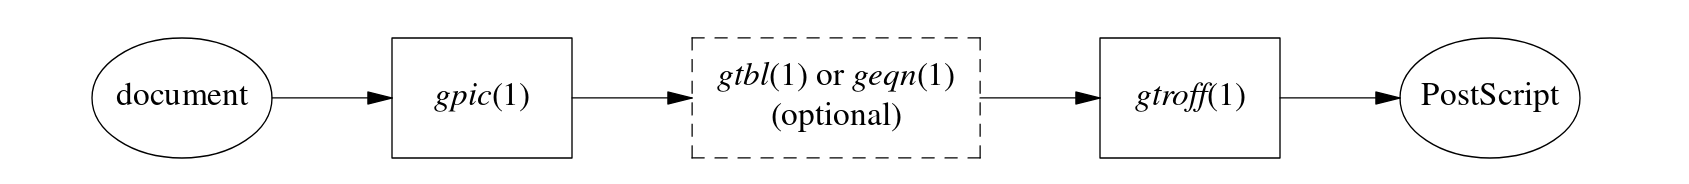
\includegraphics[width=13cm]{images/Ergebnis_1.png}
		\caption{Erzeugter Graph des Beispielcodes}
		\label{Erg_Beispielcode_1}
	\end{center}
\end{figure}

\subsection{Objekte zeichnen in PIC}

\noindent
In \textit{PIC-Code} ist es möglich verschiedene Objekte zu zeichnen. Hierbei gibt es vordefinierte Objekte, jedoch können auch neue Objekte generiert werden.
\\

\noindent
Abbildung \ref{Objekte_PIC} \footfullcite[][]{Making_Pictures_With_GNU} zeigt die grundsätzlichen Objekte von PIC:
\\
\begin{figure}[H]
	\begin{center}
		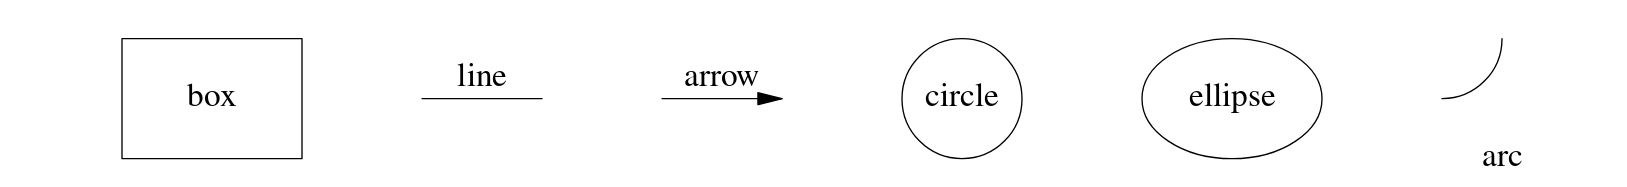
\includegraphics[width=13cm, height=2cm]{images/Objekte_PIC.png}
		\caption{Vordefinierte Objekte}
		\label{Objekte_PIC}
	\end{center}
\end{figure}

\pra

\noindent
Die Form einer Raute ist standardmäßig nicht definiert, lässt sich jedoch leicht implementieren. Es besteht nämlich die Möglichkeit, den Rand der Raute mit Hilfe von verbundenen Linien zu zeichnen. Listing \ref{list-raute} veranschaulicht die Generierung einer Raute:
\\
\noindent
\lstset{frame=lines}
\lstset{caption={Code zum Zeichnen einer Raute}}
\lstset{label={list-raute}}
\lstset{basicstyle=\footnotesize}
\begin{lstlisting}
.PS
box invis;
line from last box .n to last box .e then
to last box .s then to last box .w then to
last box .n
.PE
\end{lstlisting}

\noindent
Die generierte Raute ist in Abbildung \ref{Diamant_PIC} zu sehen.
\\
\begin{figure}[H]
	\begin{center}
		
\includegraphics[width=13cm]{images/Diamant_Beispiel.png}
		\caption{Gezeichnete Raute aus dem obigen Codebeispiel}
		\label{Diamant_PIC}
	\end{center}
\end{figure}

\noindent
\textit{PIC} verfügt über eine große Auswahl an Möglichkeiten, um ein bestimmtes Objekt zu zeichnen. Man kann durch zusätzliche Argumente zum Beispiel die Breite und die Höhe einer Box festlegen, ob der Rahmen eine durchgezogene Linie oder nur strichliert dargestellt werden soll oder ob die Box in einer bestimmten Farbe zu generieren ist. 
\\
\pra
\noindent
Der benötigte Code, um eine gelbe Ellipse zu zeichnen, wird in Listing \ref{list-Ellipse-gelb} dargestellt: 
\\
\noindent
\lstset{frame=lines}
\lstset{caption={PIC-Code zum Zeichnen einer gelben Ellipse}}
\lstset{label={list-Ellipse-gelb}}
\lstset{basicstyle=\footnotesize}
\begin{lstlisting}
.PS
ellipse shaded "yellow";
.PE
\end{lstlisting}

\noindent
Die gefärbte Ellipse wird in Abbildung \ref{Ellipse_Gelb} veranschaulicht:
\\
\begin{figure}[H]
	\begin{center}
		
\includegraphics[width=8cm]{images/Ellipse_Beispiel.png}
		\caption{Gelbe Ellipse}
		\label{Ellipse_Gelb}
	\end{center}
\end{figure}
\pra
\noindent
In \textit{PIC-Code} sind standardmäßig einige Farben vordefiniert. Es besteht jedoch auch die Möglichkeit, Farben mittels zum Beispiel hexadezimalen Werten zu definieren. Die Farbwerte können ebenfalls mit Hilfe von dem \textit{RGB}-Modell angegeben werden. Um eine neue Farbe in \textit{PIC-Code} zu definieren wird folgender Code benötigt (Listing \ref{list-farbe-def}):
\\

\noindent
\lstset{frame=lines}
\lstset{caption={Code zum Definieren einer neuen Farbe}}
\lstset{label={list-farbe-def}}
\lstset{basicstyle=\footnotesize}
\begin{lstlisting}
.PS
.defcolor medblue rgb #89D8D6
.PE
\end{lstlisting} 

\noindent
Die definierte Farbe \verb|medblue| kann so wie jede andere Farbe normal verwendet werden. Listing \ref{use-farbe} zeigt einen Beispielaufruf:
\\
\noindent
\lstset{frame=lines}
\lstset{caption={Anwendung der neu definierten Farbe}}
\lstset{label={use-farbe}}
\lstset{basicstyle=\footnotesize}
\begin{lstlisting}
.PS
    box shaded medblue;
.PE
\end{lstlisting}

\noindent
Der Code liefert als Ergebnis eine Box in einem helleren Blauton. Die Grafik wird in Abbildung \ref{Farbe_def} veranschaulicht.
\\ 
\begin{figure}[H]
	\begin{center}
		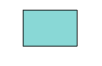
\includegraphics[width=3.5cm]{images/Box_Medblue.png}
		\caption{Box in der selbst definierten Farbe \textit{medblue}}
		\label{Farbe_def}
	\end{center}
\end{figure}
\noindent
\pra
In \textit{ERDs} müssen unter anderem auch \textit{abhängige Entitytypen} gezeichnet werden. Diese werden dargestellt, indem die Umrandung des Objektes doppelt gezeichnet wird. Das betrifft Entities und Beziehungen. 
\\

\noindent
Der Code für eine Box mit doppelt gezeichneten Linien sieht wie folgt aus(Listing \ref{list-doppelt-box}):
\\
\noindent
\lstset{frame=lines}
\lstset{caption={PIC-Code für eine Box mit doppelter Umrandung}}
\lstset{label={list-doppelt-box}}
\lstset{basicstyle=\footnotesize}
\begin{lstlisting}
.PS
boxht=1;boxwid=1;box at (0, 0);
boxht=1.2;boxwid=1.2; box at (0, 0);
.PE
\end{lstlisting}

\noindent
Abbildung \ref{Box_doppelt} zeigt das Ergebnis des oben angeführten Codes. 
\\
\begin{figure}[H]
	\begin{center}
		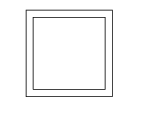
\includegraphics{images/Box_doppelt.png}
		\caption{Box mit doppelter Umrandung}
		\label{Box_doppelt}
	\end{center}
\end{figure}

\noindent
Für die Implementierung einer abhängigen Beziehung werden zwei Rauten übereinander gezeichnet, wobei eine der beiden Rauten über eine größere Höhe und Breite verfügt. In der Praxis sieht der generierte \textit{PIC-Code} wie folgt aus (siehe Listing \ref{list-doppelt-raute}):
\\
\noindent
\lstset{frame=lines}
\lstset{caption={PIC-Code zur Generierung einer Raute mit doppelter Umrandung}}
\lstset{label={list-doppelt-raute}}
\lstset{basicstyle=\footnotesize}
\begin{lstlisting}
.PS
boxht=1;boxwid=1;box invis at (0, 0);
line from last box .n to last box .e then to last box .s
then to last box .w then to last box .n;
boxht=1.2;boxwid=1.2; box invis at (0, 0);
line from last box .n to last box .e then to last box .s
then to last box .w then to last box .n;
.PE
\end{lstlisting}

\pra
\noindent
Aus diesem Code wird folgende Grafik erstellt(siehe Abbildung \ref{Raute_doppelt}):
\\

\begin{figure}[H]
	\begin{center}
		
\includegraphics{images/Raute_doppelt.png}
		\caption{Raute mit doppelter Umrandung}
		\label{Raute_doppelt}
	\end{center}
\end{figure}

\noindent
Für die Implementierung einer \textit{Super/Sub}-Beziehung muss die Form eines Dreiecks gezeichnet werden. Der benötigte Code wird in Listing \ref{dreieck-list} gezeigt:
\pra
\noindent
\lstset{frame=lines}
\lstset{caption={PIC-Code zum Zeichnen eines Dreiecks}}
\lstset{label={dreieck-list}}
\lstset{basicstyle=\footnotesize}
\begin{lstlisting}
.PS
box invis;
line from last box .n to last box .se then to last box .sw
then to last box .n
.PE
\end{lstlisting}
\noindent
Listing \ref{dreieck-list} hat folgende Ausgabe (siehe Abbildung \ref{Dreieck}) :
\\

\begin{figure}[H]
	\begin{center}
		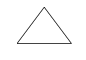
\includegraphics{images/Dreieck.png}
		\caption{gezeichnetes Dreieck von dem abgebildeten Code}
		\label{Dreieck}
	\end{center}
\end{figure}
\pra
\noindent
Ein Feature von \textit{PIC}-Code ist, dass man mit Labels arbeiten kann. Darunter versteht man, dass Objekten eine bestimmte ID zugewiesen werden kann, um im nachhinein einfach darauf zuzugreifen. Dies kann unter anderem nützlich sein, wenn zwei bestimmte Elemente verbunden werden sollen, die nicht direkt nacheinander gezeichnet wurden. Dabei sind gewisse Syntaxregeln für ein Label einzuhalten. Es darf nämlich keine Leerzeichen enthalten und muss mit einem Großbuchstaben beginnen. Weiters dürfen keine Ziffern und Umlaute vorkommen. 
\\
\pra
\noindent
\lstset{frame=lines}
\lstset{caption={Objekte mit Labels versehen und verbinden}}
\lstset{label={list-label}}
\lstset{basicstyle=\footnotesize}
\begin{lstlisting}
.PS
A: box;
move;
B: circle;
down;
move;
C: ellipse;
line from A to C;
.PE
\end{lstlisting}

\noindent
Das entstandene Bild aus Listing \ref{list-label} \footfullcite[][]{Making_Pictures_With_GNU} ist in Abbildung \ref{Label} \footnotemark[15] zu sehen.
\\

\noindent
\begin{figure}[H]
	\begin{center}
		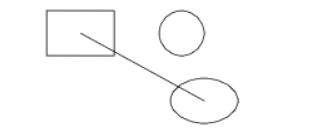
\includegraphics[width=7cm]{images/Ergebnis_Label.png}
		\caption{Objekte mit Labels versehen und verbinden}
		\label{Label}
	\end{center}
\end{figure}

\pra
\noindent
Um das Layout der gezeichneten Elemente zu bestimmen, gibt es mehrere Methoden. Wenn keine zusätzlichen Befehle angegeben werden, generiert \textit{PIC} das erste Objekt in der linken oberen Ecke des Bildes und fügt die restlichen rechts daneben ein. Es gibt jedoch die Möglichkeit, das Layout der generierten Datei mittels Addieren oder Subtrahieren der Koordinaten zu verändern und somit den Standort der Graphen zu bestimmen. Eine weitere Art der Spezifizierung kann dadurch erreicht werden, indem x- und y-Werte direkt in den Befehl eingebunden werden. In Listing \ref{list-kord} ist ein Beispiel abgebildet, wie Objekte an bestimmten Koordianten gezeichnet werden.
\\

\noindent
\lstset{frame=lines}
\lstset{caption={PIC-Code zur Generierung einer Box an den Koordinaten [100, 100]}}
\lstset{label={list-kord}}
\lstset{basicstyle=\footnotesize}
\begin{lstlisting}
.PS
A:box at (100, 100);
.PE
\end{lstlisting}

\noindent
Um den \textit{Primary Key} von einem \textit{Entity} zu bestimmen, muss der Inhalt des \textit{Primary-Key}-Attributes unterstrichen werden. Dies wird in \textit{PIC}-Code implementiert, indem 2 Ellipsen übereinander gezeichnet werden, wobei in einer Ellipse der Name des \textit{Attributes} steht und in der zweiten Ellipse befinden sich anstatt eines Textes als Name mehrere aufeinanderfolgende Unterstriche. Der Code, um dieses Ergebnis zu erzielen, wird in Listing \ref{list-unter} veranschaulicht:
\pra
\lstset{frame=lines}
\lstset{caption={PIC-Code zum Unterstreichen von Text in einer Ellipse]}}
\lstset{label={list-unter}}
\lstset{basicstyle=\footnotesize}
\begin{lstlisting}
.PS
ellipse "Unterstrichen";
ellipse at last ellipse "__________";
.PE
\end{lstlisting}

\noindent
Aus Listing \ref{list-unter} wird folgende Grafik erzeugt (siehe Abbildung \ref{Unterstrichen})):

\noindent
\begin{figure}[H]
	\begin{center}
		
\includegraphics[width=3.5cm]{images/Ellipse_unterstrichen.png}
		\caption{Text der Ellipse wird unterstrichen}
		\label{Unterstrichen}
	\end{center}
\end{figure}

\noindent
Weiters müssen die \textit{Primary Keys} von \textit{abhängigen Entities} mit einer strichlierten Linie unterstrichen werden. Der \textit{PIC-Code} zur Darstellung eines Attributes mit einem strichliert unterstrichenem Text sieht wie folgt aus (Listing \ref{list-unterstr}):

\lstset{frame=lines}
\lstset{caption={Text der Ellipse wird strichliert unterstrichen}}
\lstset{label={list-unterstr}}
\lstset{basicstyle=\footnotesize}
\begin{lstlisting}
.PS
ellipse "Unterstrichen";
ellipse at last ellipse "_ _ _ _ _ _";
.PE
\end{lstlisting}

\noindent
Der in Listing \ref{list-unterstr} gezeigte Code generiert folgende Grafik (siehe Abbildung \ref{strichl_unter}):
\begin{figure}[H]
	\begin{center}
		
\includegraphics[width=3.5cm]{images/Ellipse_strichliert.png}
		\caption{Text der Ellipse wird strichliert unterstrichen dargestellt}
		\label{strichl_unter}
	\end{center}
\end{figure}

\subsubsection{Anpassen der Objekte}
\pra

\noindent
In \textit{PIC}-Code steht die Option zur Verfügung, dass Eigenschaften von Objekten wie zum Beispiel von Boxen, Ellipsen oder von Kreisen per Hand hinzugefügt werden können. Dies betrifft unter anderem die Höhe und die Breite. Weiters können Attribute für das ganze Dokument angegeben werden, wie zum Beispiel die maximale Höhe und Breite von dem gesamten Bild. Standardmäßig sind diese Werte bei Boxen und Ellipsen 0.5 cm und 0.75 cm. Der Radius für einen Kreis beträgt 0.25 cm, falls dieser nicht angegeben wird. 
\\

\noindent
Um die Breite und die Höhe beispielsweise auf jeweils 4 Zentimeter zu setzen, muss der Code wie folgt aussehen (siehe Listing \ref{list-wid-ht}):

\lstset{frame=lines}
\lstset{caption={Setzen der Boxbreite und -höhe auf 4cm}}
\lstset{label={list-wid-ht}}
\lstset{basicstyle=\footnotesize}
\begin{lstlisting}
.PS
quadrat: boxwid=4;boxht=4; box;
.PE
\end{lstlisting}

\noindent
Es gibt ausserdem die Option, ein bestimmtes Objekt zu skalieren. Diese kann hilfreich sein, wenn die Grenzen des zu generierenden Bildes sehr groß sind. Listing \ref{list-scale} zeigt, wie der Skalierungsfaktor einer Box gesetzt werden kann:

\lstset{frame=lines}
\lstset{caption={Setzen des Skalierungsfaktors einer Box auf 15}}
\lstset{label={list-scale}}
\lstset{basicstyle=\footnotesize}
\begin{lstlisting}
.PS
scaledbox: scale=15; box;
.PE
\end{lstlisting}

\subsection{Layout}
\label{layout}
\pra
\noindent
Das Layout des ganzen Diagrammes wird mit Hilfe von \verb|graphviz-layout| erzeugt. 

\noindent
Der Python-Code für die Generierung der Koordinaten wird in Listing \ref{list-python-layout} gezeigt:
\\
\lstset{language=Python}
\lstset{frame=lines}
\lstset{caption={Python Code zur Generierung des Layouts mittels graphviz-layout}}
\lstset{label={list-python-layout}}
\lstset{basicstyle=\footnotesize}
\begin{lstlisting}
def nx_graph(rel):
    erd = nx.Graph()
    for curr in rel:
        if len(curr) > 1:
            for i in range(len(curr)):

                erd.add_edge(curr[0], curr[i])
        else:
            continue
    pos = graphviz_layout(erd, prog='neato', args="-Gsplines=true -Goverlap=scale -Gsize=100,200! -Gmaxiter=10000 -Gepsilon=0.00001 -Gdpi=1 -Gratio=fill" )
    return pos
\end{lstlisting}

\noindent
Der Befehl \verb|graphviz_layout| verfügt über einige Parameter, die das zu generierende Layout bestimmen. Das Argument \verb|prog| gibt den Algorithmus für das Layout an. Als gültige Parameter dieses Arguments gelten \footfullcite{graphviz_visualization}: 
\\

\begin{itemize} \pra 
	\item{\verb|dot|} kann sinnvoll verwendet werden, wenn das gewünschte Ergebnis hierarchisch oder geschichtet dargestellt werden soll.
	\item{\verb|neato|} produziert die Grafik gemäß des \textit{Sprungfedermodells}. Dieser Parameter ist der Standard für ungerichtete Graphen.
	\item{\verb|twopi|} erstellt für gerichtete und ungerichtete Graphen eine Darstellung, bei der die Knoten radial angeordnet werden.
	\item{\verb|fdp|} beinhaltet einen Mehrgitterlöser zur Behandlung von großen und geclusterten Graphen.
	\item{\verb|sfdp|} ist eine skalierbare Version von \verb|fdp|. Diese Option eignet sich besonders gut für große Diagramme.
	\item{\verb|circo|} ordnet die Knoten kreisförmig an. Dieser Parameter erweist sich als sinnvoll für bestimmte Diagramme von mehrfach zyklischen Strukturen.
\end{itemize}

\noindent
Jeder dieser Layoutalgorithmen hat seine Vorteile, jedoch bietet \verb|neato| angewendet auf alle Datenmodelle das bestgeeignetste Layout für ein \textit{Entitiy Relationship Diagramm} mit den wenigsten Überschneidungen der Linien.
\\

\noindent
Es können weitaus mehr Layoutalgorithmen angegeben werden, jedoch sind die oben aufgezählten Parameter am Sinnvollsten beziehungsweise erstellen diese Algorithmen ein \textit{Entity Relationship Diagramm} in einem gut lesbaren Layout. 
\\

\noindent
Die Argumente des Parameters \verb|args| sind Zusatzeinstellungen, die für die Generierung der Grafik nützlich sind. Unter anderem kann als Attribut \verb|-Gsize| angegeben werden um die Größe des Dokuments zu bestimmen. Weitere Argumente sind zum Beispiel \verb|-Gsplines|
\verb|-Goverlap, -Gmaxiter, -Geplsilon, -Gdpi| und \verb|-Gratio|.
\\

\subsection{Erstellen einer PIC-Datei}
\pra

\noindent
Der \textit{Python}-Code, indem die \textit{PIC}-Datei erstellt und beschrieben wird, sieht wie folgt aus (Listing \ref{list-pic-file}):

\lstset{language=Python}
\lstset{frame=lines}
\lstset{caption={Python Code, indem der generierte PIC-Code in eine selbsterstellte PIC-Datei geschrieben wird}}
\lstset{label={list-pic-file}}
\lstset{basicstyle=\footnotesize}
\begin{lstlisting}
def write_erd_to_file(pic):

    if os.path.exists("erd.pic"):
        os.remove("erd.pic")
    file = open("erd.pic", "w")
    file.write(pic)  
    file.close()
    print('Your file is created at: ' + os.getcwd() + '/erd.pic')

\end{lstlisting}

\noindent
Der Parameter \textit{pic} ist der generierte \textit{PIC}-Code, der das \textit{ERD} zeichnet.

\noindent
Sobald in das erstellte Dokument der \textit{PIC}-Code ergänzt wurde, kann die Datei kompiliert und angezeigt werden.

\subsection{Vorteile und Nachteile von PIC}
\pra

\subsubsection{Vorteile}

\noindent
Die Erweiterung \textit{PIC} bietet einige Vorteile, die für die Generierung von Dokumenten und Graphen hilfreich sein können:
\\
\begin{itemize}
	\item Da die Sprache sehr einfach aufgebaut ist und die Namen der Befehle bzw. Objekte sprechend gewählt wurden, fällt es einem späteren Leser nicht schwer, den Code zu verstehen. Vor allem mit Hilfe der vordefinierten Objekte wird das Generieren grundlegender Graphen um einiges vereinfacht und erfordert keinen großen Aufwand.
	\lstset{frame=lines}
	\lstset{caption={Leicht lesbarer Code zur Generierung einer Grafik}}
	\lstset{label={list-corde-lesbar}}
	\lstset{basicstyle=\footnotesize}
	\begin{lstlisting}
.PS
box "from"
move 0.75;
ellipse "to";
arc cw from 1/3 of the way \
 between last box .n and last box .ne to last ellipse .n;
.PE
	\end{lstlisting}
	
	\noindent
	Aus Listing \ref{list-corde-lesbar}\footfullcite[][]{Making_Pictures_With_GNU} wird folgende Grafik erzeugt(sieht Abbildung \ref{SprechendName} \footnotemark[17]):
	\begin{figure}[H]
		\begin{center}
			
\includegraphics[width=13cm]{images/PIC_Aufbau_Einfachkeit.png}
			\caption{Ergebnis des Codes}
			\label{SprechendName}
		\end{center}
	\end{figure}
	
	\item Weiters kann man dank der Fehlermeldungen und des leicht zu lesenden Codes sowohl syntaktische als auch logische Fehler ohne großem Aufwand finden und beheben.


\end{itemize}

\subsubsection{Nachteile}
\pra

\noindent
Neben den Vorteilen gibt es jedoch auch Nachteile, die im Vergleich zu den Pro-Argumenten überwiegen. Zu den negativen Aspekten zählen:

\begin{itemize}
	\item Die Anzahl der standardmäßig definierten Objekte in \textit{PIC} ist nur gering. Daraus folgt, dass der Aufwand andere Objekte zu zeichnen steigt, auch wenn das nur geringfügig bzw. der Code leicht zu generieren ist. \textit{PIC} verfügt zwar über die Möglichkeit, Makros zu definieren, jedoch ist die Definition dieser Makros ein Aufwand, der bei den anderen Implementierungsvarianten nicht existiert, da dort die benötigten Objekte bereits vordefiniert sind.
	\\
	\pra
	\item Weiters ist über \textit{PIC}-Code zu sagen, dass das Verbinden von zwei unterschiedlichen Objekten in der Theorie recht einfach ist, praktisch jedoch nur mit viel Aufwand verbunden umgesetzt werden kann. Es müssen nämlich die Bezugspunkte (Norden, Osten, Süden, Westen) angegeben werden, denn ohne diese Information befinden sich der Beginn und das Ende der gezeichneten Linie in der Mitte des jeweiligen Objektes. Falls dieser Gegenstand eine Beschriftung aufweist, hat dies zur Folge, dass der Inhalt der Box schwerer bis nicht mehr lesbar wird. Dies ist insofern ein Nachteil, da das Verbinden der Objekte viele Abfragen benötigt, weil der Start- und der Endpunkt nicht sofort bekannt sind. Die Koordinaten der zwei zu verbindenden Elemente müssen zuerst verglichen werden, um dann die richtigen Bezugspunkte zu wählen. 
	Ohne diese Abfragen sieht die Verbindung zwischen zwei Boxen aus wie in Abbildung \ref{ConnProb} zu sehen ist.
	\begin{figure}[h!]
		\begin{center}
			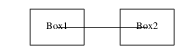
\includegraphics[width=7cm]{images/Connectoren_Problem.png}
			\caption{Konnektoren ohne zusätzlicher Information über Start- und Endpunkt}
			\label{ConnProb}
		\end{center}
	\end{figure}

	\noindent
	\textit{PIC}-Code unterscheidet sich in diesem Punkt von \textit{Graphviz, Libre Office Draw} und \textit{Graphml}. Bei den Varianten werden die Bezugspunkte automatisch gesetzt.
	\\
	
	\item 
	Die Generierung des Layouts des ganzen Diagrammes stellt generell ein großes Problem dar. Mittels \textit{PIC}-Code ist es nicht möglich, ein gut aussehendes \textit{ERD} zu erzeugen. Daher muss mit Hilfe von \textit{Graphviz} das Layout im vorhinein generiert werden, wobei nur die Koordinaten der Knoten erzeugt werden und nicht das ganze Diagramm. Ausgehend von diesen Werten können dann die Objekte einfach im \textit{PIC}-Code positioniert werden (siehe Kapitel \ref{layout}). 
	\pra
	\noindent
	Auf Grund dieser Methode tritt ein weiteres Problem auf und zwar, dass man beim Generieren der Koordinaten die richtigen Parameter für den Befehl \verb|graphviz_layout| benötigt. Diese müssen mit dem Dokument übereinstimmen, da sonst die Werte der Koordinaten zu groß werden und deswegen Elemente ausserhalb des Dokuments gezeichnet werden. Ausserdem erzeugt dieser Befehl die generierten Punkte in einem viel zu großen Ausmaß, sodass die Werte trotz richtigen Parametern noch bearbeitet werden müssen.
	\\
	
	\item Bei der Generierung des Layouts treten häufig Probleme auf. Das liegt daran, dass PIC die Koordinaten in \textit{inches} berechnet, jedoch eine PDF Datei mit Pixel arbeitet. Dies erschwert das Generieren mittels absoluten Koordinaten, da von PIC nicht überprüft wird, ob der Wert noch innerhalb des anzeigbaren Bereiches liegt oder ob dieser ausserhalb des gegebenen Bereiches gezeichnet wird. Dies kann zur Folge haben, dass ein Objekt teilweise abgeschnitten wird, wie in der Abbildung \ref{Box_Cut} zu sehen ist.
	\\
	
	\lstset{frame=lines}
	\lstset{caption={PIC-Code, um den Fehlerfall zu zeigen, dass eine Box bei zu großen Koordinaten abgeschnitten wird}}
	\lstset{label={list-box-cut}}
	\lstset{basicstyle=\footnotesize}
	\begin{lstlisting}
	.PS
	box at (0, 300);
	.PE
	\end{lstlisting}
	
	\noindent
	Listing \ref{list-box-cut} wird in Abbildung \ref{Box_Cut} veranschaulicht:
	\noindent
	\begin{figure}[H]
		\begin{center}
			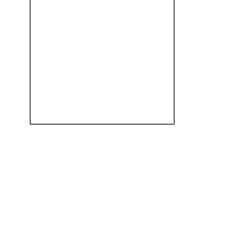
\includegraphics[scale=0.5]{images/Erg_Code_abgeschnitten.png}
			\caption{Box wird wegen zu großen Koordinaten abgeschnitten}
			\label{Box_Cut}
		\end{center}
	\end{figure}
\pra
	Wenn die Koordinaten zu groß werden, kann es auch zu dem Fall kommen, dass diese nicht einmal mehr in der Nähe der maximalen Grenzen liegen. Das hat zur Folge, dass das Element nicht mehr angezeigt werden kann. 
	\\
	\lstset{frame=lines}
	\lstset{caption={Code, um den Fehlerfall zu erzeugen, dass eine Box ausserhalb des sichtbaren Bereiches gezeichnet wird}}
	\lstset{label={list-err}}
	\lstset{basicstyle=\footnotesize}
	\begin{lstlisting}
	.PS
	box at(500, 0)
	boxwid=35;boxht=15;  bot at (0, 0);
	line from 1st box to last box;
	\end{lstlisting}
	\noindent
	Die generierte Grafik wird in Abbildung \ref{Box_Away} verbildlicht. \pra
	\begin{figure}[h!]
		\begin{center}
			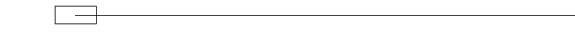
\includegraphics{images/ERG_Box_weg.png}
			\caption{Box wird wegen zu großen Koordinaten ausserhalb des Sichtfeldes gezeichnet}
			\label{Box_Away}
		\end{center}
	\end{figure}
	\\	
\end{itemize}


\newpage
\section{yEd}
\label{yed}
\prc

Das Programm yEd ist ein Graph Editor, mit dem die verschiedensten Diagrammtypen erstellt werden können. Die Applikation wurde von dem deutschen Unternehmen yWorks entwickelt und basiert auf der Java-Bibliothek yFiles. Dadurch punktet der Editor nicht nur mit den Layout-Algorithmen und den Analyse-Tools die durch die Bibliothek zur verfügung gestellt werden sondern auch mit einem übersichtlichen User-Interface, dass das erstellen und bearbeiten von Diagrammen vereinfacht.
\\

\subsection{Varianten und Installation}

\noindent
Um die Anwendung zu nutzen gibt es zwei Möglichkeiten. Die erste wäre den ,,yEd Live''-Dienst in Anspruch zu nehmen. Dabei handelt es sich um eine Online-Variante. Der Nachteil dieses Services ist, dass die Verarbeitung und auch Darstellung der Daten im Hintergrund anders ist als bei der Offline-Version. Dies führt unter anderem dazu, dass die erzeugten GraphMl-Dateien bei ,,yEd Live'' nicht richtig bis hin zu gar nicht angezeigt werden.
\\

\noindent
Bei der zweiten Methode handelt es sich um die Offline-Version. Diese kann über die offizielle Internetseite von yWorks für das entsprechende Betriebssystem heruntergeladen und danach entsprechend installiert werden.
\\

\noindent
Wichtig ist es bei der Auswahl der Datei für die Installation darauf zu achten, ob diese auch die benötigte Java JRE beinhaltet und wenn nicht, ob man selbst auf dem Rechner die dazugehörige installiert hat. Wenn man sich dann im Installationsprozess befindet kommt man an einen Punkt, an dem man nach einem Installationspfad gefragt wird. Hierbei muss man darauf achten das Programm an einem Ort zu installieren zu dem man als Benutzer auch Zugriff hat, weil das Command-Line-Tool bei der Erstellung eines ER-Diagrammes anbietet, die generierte Grafik, sofern es sich um eine GraphMl Datei handelt und man auf Linux arbeitet, direkt von der Kommandozeile heraus in yEd zu öffnen.

\begin{figure}[!h]
	\begin{center}
		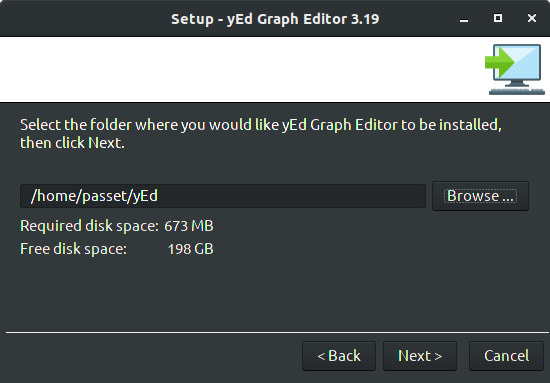
\includegraphics[width=10cm]{images/yed_installation_pfad.png}
		\caption{Angabe des Installationspfades im Installer von yEd 3.19}
		\label{yEdInstaller}
	\end{center}
\end{figure}

\subsection{Oberfläche}
\prc

\noindent
Das grafische Interface mit dem der Benutzer interagiert entspricht zwar nicht den modernsten Design Ideen aber bietet alles was man braucht. Grundlegend kann man die Oberfläche des Editors in 7 Bereiche unterteilen.

\subsubsection{Menü}

Den Kopf der Oberfläche bildet das Menü. Hier kann der Benutzer verschiedene Ansichten und Funktionen aktivieren bzw. deaktivieren. Es umfasst die Menüs Datei, Bearbeiten, Ansicht, Layout, Werkzeuge, Gruppierung, Fenster und Hilfe.

\subsubsection{Palette}

\noindent
In der Palette befinden sich die Elemente mit denen man einen Graphen erstellen kann. Diese Komponenten sind in Gruppen aufgeteilt um für einen besseren Überblick zu sorgen. Zu Beginn bietet der Editor einem die folgenden Gruppierungen mit den entsprechenden Elementen:
\\

\begin{multicols}{2}
    \begin{itemize}
        \item Geometrische Knoten
        \item Moderne Knoten
        \item Kantentypen
        \item Gruppenknoten
        \item Swimlane- und Tabellenknoten
        \item Personen
        \item Computer-Netzwerk
        \item UML
        \item Flussdiagramm
        \item BPMN 
        \item Entity Relationship
        \item SBGN
        \item Aktuelle Elemente
        \\
    \end{itemize}
\end{multicols}

\noindent
Es gibt auch für den Benutzer die Möglichkeit selbst eine Gruppe mit Elementen zu erstellen und diese dann auch in die Palette einzubinden \footfullcite{yEdManual}. 

\begin{figure}[H]
	\begin{center}
		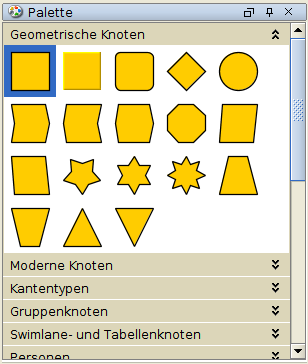
\includegraphics[width=5cm,height=6cm]{images/yed_palette_offen.png}
		\caption{Palette in yEd bei Programmstart}
		\label{yEdPaletteOffen}
	\end{center}
\end{figure}

\subsubsection{Eigenschaften}
\prc

\noindent
Der Bereich Eigenschaften zeigt die charakteristischen Werte des momentan ausgewählten Elementes an. Hier können allerlei verschiedener Veränderungen vorgenommen werden wie zum Beispiel das Ändern der Beschreibung, Größe oder auch Farbe, vorausgesetzt natürlich das diese änderbar sind. Die Merkmale in diesem Bereich werden in die Gruppen Allgemein, Beschriftung, Daten und eine für das Element spezifische Gruppe aufgeteilt. In der Abbildung \ref{yEdEigenschaften} wäre dann die spezifische Gruppe ,,Entity Relationship''.

\begin{figure}[!h]
	\begin{center}
		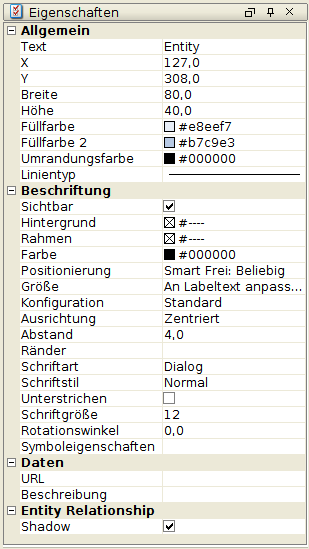
\includegraphics[width=6.5cm,height=10cm]{images/yed_eigenschaften.png}
		\caption{Eigenschaften eines Entitytypen in yEd}
		\label{yEdEigenschaften}
	\end{center}
\end{figure}

\noindent
Sollte man kein Element seines Graphen ausgewählt haben, sieht man in diesem Bereich die Gesamtzahl an Knoten und Kanten. 

\subsubsection{Nachbarschaft}

\noindent
Auf der linken Seite der GUI befinden sich Bereiche die einem Auskunft über den Aufbau des aktuellen Graphen geben. Darunter befindet sich der Bereich Nachbarschaft. In diesem Fenster sieht man demnach alle Nachbar-Knoten des momentan ausgewählten Knoten. Zudem bietet es Registerkarten an, in denen nur die Knoten innerhalb der Gruppe, Vorgänger oder Nachfolger angezeigt werden. 
\\

\noindent
Dies kann sich bei einem Entity-Relationship Diagramm als großen Vorteil entpuppen, da mit einem Klick herausgefunden werden kann mit welchen Beziehungstypen der Entitytyp in relation steht. In der Abbildung \ref{yEdNachbarschaft} wird die Nachbarschaft des Entitytypen Abteilung dargestellt.

\begin{figure}[!h]
	\begin{center}
		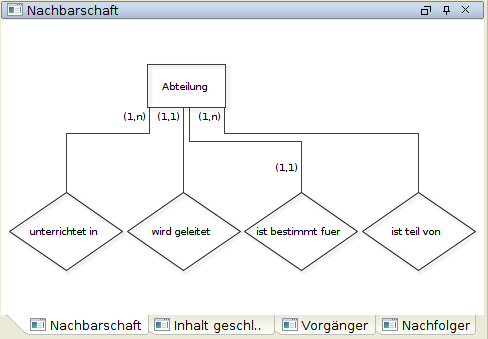
\includegraphics[width=10cm]{images/yed_nachbarschaft.png}
		\caption{Nachbarschaft des Entitytypen Abteilung aus dem Datenmodell Schulinformationssystem}
		\label{yEdNachbarschaft}
	\end{center}
\end{figure}

\subsubsection{Struktur}
\prc
Im wesentlichen beinhaltet dieser Bereich eine Liste mit all den Elementen die sich zum momentanen Zeitpunkt auf der Hauptoberfläche von yEd befinden. Sie ist hierarchisch geordnet, weshalb Teile des Graphen die zuerst erstellt wurden weiter oben angeführt sind als Teile die später hinzugefügt wurden. 
\\

\noindent
Das Fenster Struktur ist eng mit den zuvor genannten Bereichen verbunden. Wählt man eine der Komponenten aus wird sie im Graphen markiert, die Eigenschaften dargestellt und die Nachbarschaft aufgezeigt.

\begin{figure}[H]
	\begin{center}
		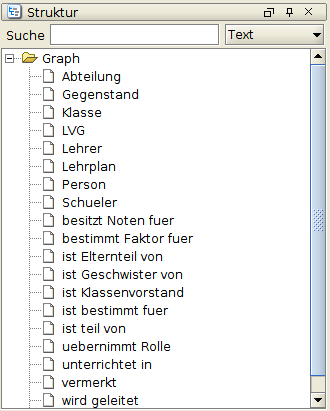
\includegraphics[width=6.5cm,height=7.5cm]{images/yed_struktur.png}
		\caption{Strutkur des ER-Diagrammes Schulinformationssystem}
		\label{yEdStruktur}
	\end{center}
\end{figure}

\subsubsection{Editor-Bereich}
\prc

In diesem Bereich wird der Graph dargestellt und durch Elemente aus der Palette ergänzt und verändert. Dies geschieht durch die Verwendung einer Maus oder durch drücken bestimmter Tasten auf der Tastatur. Die folgenden Aktionen und noch weiter nicht angeführte können auf diese Weise ausgeführt werden:
\\

\begin{itemize}
    \item Einen neuen Knoten erstellen und auswählen
    \item Eine Kante erstellen und auswählen
    \item Knoten verschieben
    \item Eine neuen Biegepunkt auf der Kante erstellen und verschieben
    \item Ein Element löschen
    \item Eine Beschriftung erstellen, auswählen, bearbeiten und verschieben
    \\
\end{itemize}

\noindent
Die folgende Abbildung zeigt einen von yEd generierten Graphen den man ohne weiteres durch die Verwendung der eben genannten Aktionen erstellen kann.

\begin{figure}[H]
	\begin{center}
		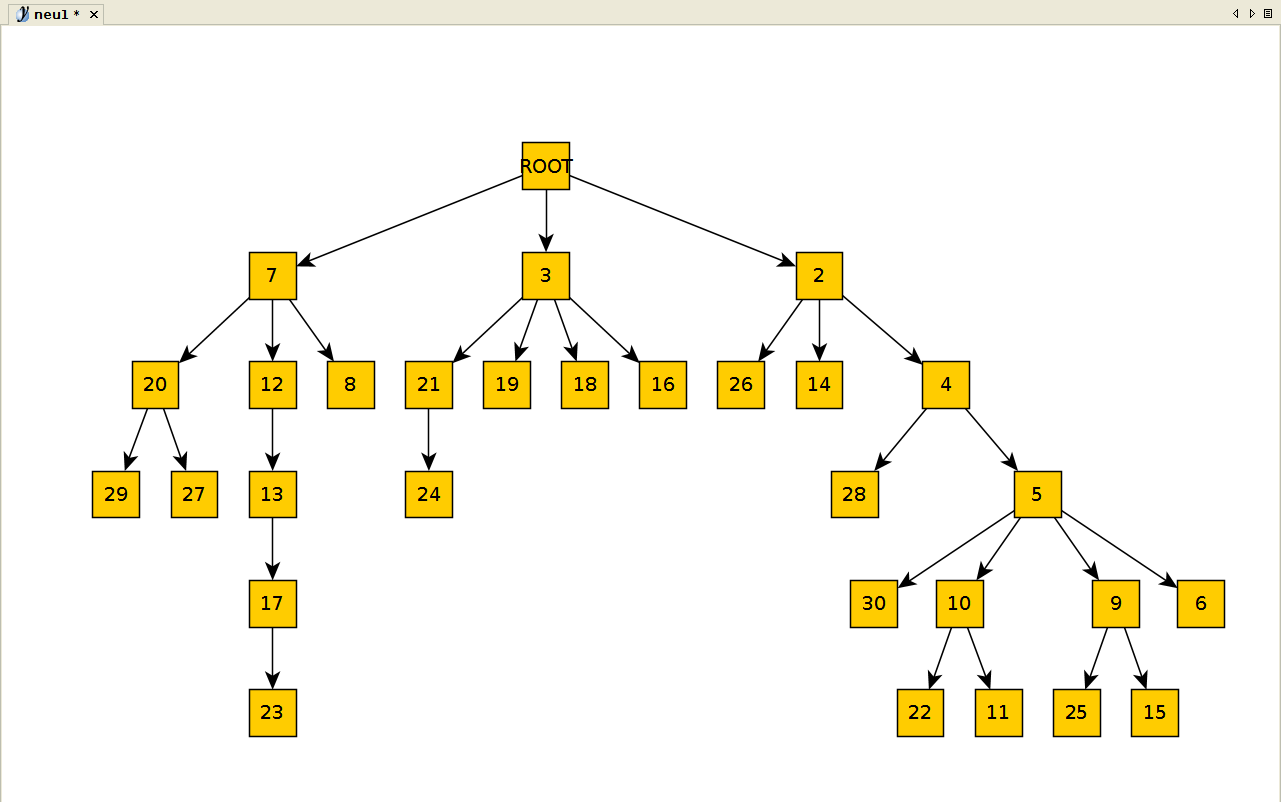
\includegraphics[width=13cm,height=10cm]{images/yed_editor.png}
		\caption{Beispiel Graph generiert von yEd}
		\label{yEdEditor}
	\end{center}
\end{figure}

\subsubsection{Übersicht}

Den letzten Bereich der Oberfläche bietet die Übersicht. Hier wird der gesamte Graph dargestellt. Sollte der Editor-Bereich nicht den ganzen Graphen anzeigen wird in der Übersicht durch eine weiße Form gezeigt was gerade im Editor-Bereich angezeigt wird. Diese Form kann mit dem Mauszeiger durch anklicken und bewegen verschoben werden. Auf diese Weise kann man im Editor-Bereich navigieren.


\subsection{Editier-Hilfen}

Um den Benutzer bei der Anordnung der Elemente seines Graphen zu unterstützen, bietet yEd 3 Features.

\subsubsection{Snap Lines}
\prc
Im \citetitle{yEdManual} wird das Grundkonzept der ,,Snap Lines'' , zu deutsch Hilfslinien, wie folgt beschrieben:

\begin{quote}
    Snap Lines help you to interactively create a graph with an appealing layout.
\end{quote}

\noindent
Zusammenfassend lässt sich also sagen, dass die ,,Snap Lines'' für ein ansprechendes Layout sorgen. Diese Linien werden angezeigt während man ein ausgewähltes Element bewegt. Dabei rastet die Komponente an den Stellen ein wo es gut aussehen könnte und zeigt durch eine Linie an, weshalb es dort eingerastet ist.
\\

\noindent
In der Abbildung \ref{snapLineCenter} sieht man zum Beispiel, dass das ausgewählte Element an dieser Stelle einrastet weil es sich auf der selben Höhe befindet wie das Element das nebenan platziert ist.

\begin{figure}[!h]
	\begin{center}
		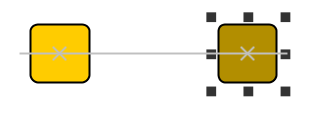
\includegraphics[width=10cm]{images/yed_snap_center.png}
		\caption{,,Snap Line'' hilft bei der zentralen Positionierung}
		\label{snapLineCenter}
	\end{center}
\end{figure}

\noindent
Des Weiteren lassen die ,,Snap Lines'' einen erkennen, ob ein Knoten der zwischen 2 anderen Knoten positioniert wird sich mittig befindet oder ob ein Knoten die selbe Höhe oder Breite hat als ein anderer Knoten.

\subsubsection{Grid}

Eine weitere Hilfestellung für ein gutes Layout ist das Grid, zu deutsch Gitter, das man über die Menüleiste einschalten kann. Hat man es eingeschaltet, rasten die Elemente die man aus der Palette zieht an einem der fest vorgegebenen Punkte ein.

\subsubsection{Orthogonale Kanten}

Das letzte Feature das Abhilfe bei der händischen Anordnung der Komponenten schafft sind die orthogonalen Kanten. Hat man diese Funktion über die Menüleiste von yEd aktiviert, dann werden Kanten nur noch mit 90° Winkeln erstellt. Das heißt, dass es keine schiefen Linien mehr gibt, sondern der Editor von sich aus die Linien horizontal bzw. vertikal zeichnet bis die gewünschten Knoten miteinander verbunden sind, wie in Abbildung \ref{yedOrthogonaleKante} dargestellt wird.

\begin{figure}[H]
	\begin{center}
		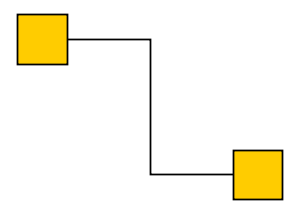
\includegraphics[width=5.5cm]{images/yed_ortogonale_kante.png}
		\caption{Beispiel einer orthogonalen Kante in yEd}
		\label{yedOrthogonaleKante}
	\end{center}
\end{figure}

\subsection{Layout-Algorithmen}
\prc

Einer der größten Vorteile die yEd besitzt, sind die Layout-Algorithmen die der Editor einem zur Verfügung stellt. Insgesamt kann man zwischen 19 verschiedenen auswählen. Diese sind unter anderem: 

\begin{multicols}{2}
	\begin{itemize}
		\item Hierarchisch
		\item Organisch
		\item Orthogonal
		\begin{itemize}
			\item Klassich
			\item UML-Stil
			\item Kompakt
		\end{itemize}
		\item Kreisförmig
		\item Baumartig
		\begin{itemize}
			\item Gerichtet
			\item Ballon
		\end{itemize}
		\item Radial
		\item Serien-Parallel
		\item Swimlane
		\begin{itemize}
			\item Hierarchisch
			\item Organisch
			\item Tabellarisch
		\end{itemize}
		\item Flowchart
		\item BPMN
		\item SBGN
		\item Stammbaum
		\item Tree-Map
		\item One-Click Layout
	\end{itemize}
\end{multicols}

\noindent
Der Benutzer hat natürlich die freie Wahl welches Layout er für sein Diagramm haben möchte aber im \cite{yEdManual} sind Empfehlungen gelistet welcher Algorithmus für welchen Diagrammtyp am besten geeignet ist. In den folgenden Unterkapiteln werden jene Layouts näher beschrieben die für ein ER-Diagramm geeignet sind.

\subsubsection{Orthogonales Layout}

Für Entity-Relationship-Diagramme wird das \textit{Orthogonale Layout} empfohlen. Davon stehen 3 Varianten zur Auswahl:
\\

\begin{itemize}
	\item Klassisch
	\item UML-Stil
	\item Kompakt
	\\
\end{itemize}

\noindent
Jede dieser Methoden verfügt über unterschiedliche Parameter die man als Benutzer festlegen kann und die anschließende Darstellung sichtlich beeinflussen. In der nachfolgenden Abbildung \ref{sisOrthogonalKlassisch} wird ein Beispiel von einem Datenmodell gezeigt, dessen Elemente mithilfe des klassischen Orthagonalen Layout angeordnet wurden.

\begin{figure}[H]
	\begin{center}
		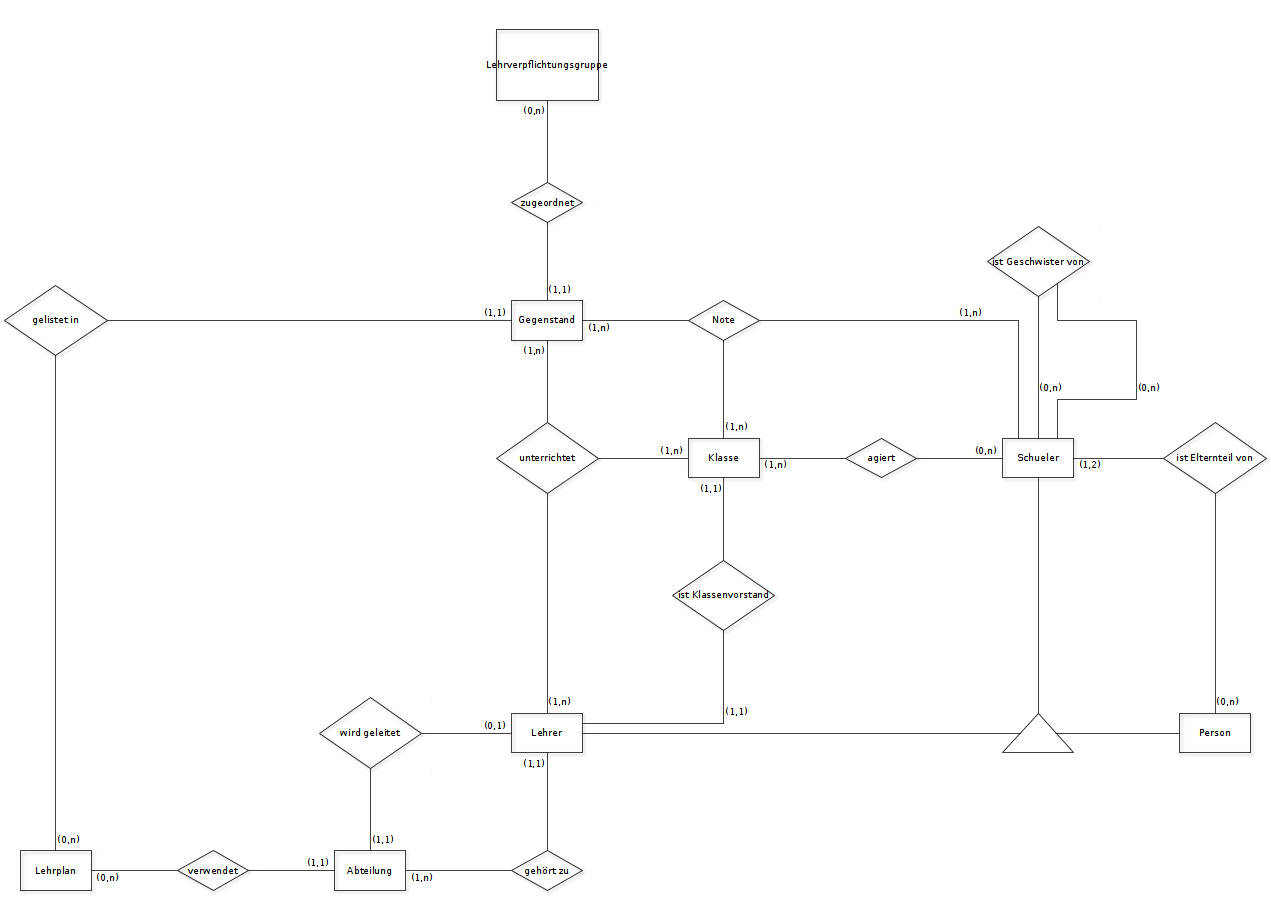
\includegraphics[width=8cm]{images/sisOrthagonal.png}
		\caption{Beispiel für die Anordnung durch klassisches Orthogonales Layout}
		\label{sisOrthogonalKlassisch}
	\end{center}
\end{figure}

\noindent
Wie man sehen kann sind die Kanten alle gerade weshalb es schön anzusehen und auch lesbar ist. Zeichnet man jedoch auch die Attribute in das Diagramm werden wie in Abbildung \ref{orthogonalKlobig} ersichtlich, viele Kanten nah aneinander gelegt, was das Diagramm klobig erscheinen lässt.

\begin{figure}[H]
	\begin{center}
		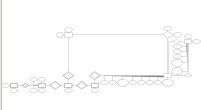
\includegraphics[width=10cm]{images/orthogonalAttribute.png}
		\caption{Orthogonales Layout mit Attributen }
		\label{orthogonalKlobig}
	\end{center}
\end{figure}

\subsubsection{Kreisförmig}
\prc

Im Zuge der Diplomarbeit wurde auch das \textit{Kreisförmige Layout} näher untersucht. Wie der Name schon preisgibt, werden hierbei die Knoten in einem oder mehrere Kreise angeordnet abhängig von den Einstellungen. Bei diesem Layout werden 4 Stile unterschieden:
\\

\begin{itemize}
	\item BCC Kompakt
	\item BCC isoliert
	\item Benutzerdefinierte Gruppen
	\item Einzelner Kreis
\end{itemize}

\noindent
\prc
Für ein ER-Diagramm könnte man die Stile BCC Kompakt und BCC isoliert in betracht ziehen. Bei BCC Kompakt repräsentieren die Teile des Diagramms \textit{biconnected} Komponenten. Diese Komponente wird laut \citetitle{yEdManual} wie folgt definiert:

\begin{quote}
	A biconnected component consists of nodes that are reachable by two edge disjoint paths.
\end{quote}

\noindent
Sollte ein Knoten die Möglichkeit haben zu zwei Komponenten zu gehören wird dieser vom Algorithmus einer Komponente exklusiv zugewiesen.
\\

\noindent
BCC isoliert wendet das selbe verfahren an wie BCC Kompakt. Kommt es hierbei jedoch zu dem Fall, dass ein Knoten zu zwei Komponenten dazugehören könnte wird dieser als eingene Komponente im Diagramm dargestellt \footcite{yEdManual}.
\\

\noindent
Wie man an den Abbildungen \ref{bccKompaktFlug} und \ref{bccIsoliertFlug} erkennen kann, ist es möglich ein ER-Diagramm mit diesem Algorithmus gut darzustellen bzw. es mit wenigen Handgriffen über die Editor-Oberfläche zu verschönern. Jedoch kann sich, abhängig von dem jeweiligen Datenmodell, ein Diagramm wie in Abbildung \ref{bccKompaktSis} entstehen.

\begin{figure}[!h]
	\begin{center}
		\subfigure[Datenmodell Fluggesellschaft mit BCC Kompakt]
		{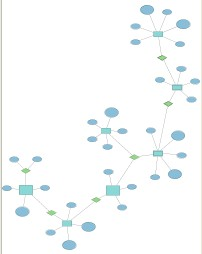
\includegraphics[width=6cm,height=9cm]{images/fluggesellschaftBccKompakt.png}
		\label{bccKompaktFlug}}
		\subfigure[Datenmodell Fluggesellschaft mit BCC isoliert]
		{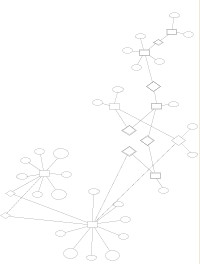
\includegraphics[width=6cm,height=9cm]{images/fluggesellschaftBccIsoliert.png}
		\label{bccIsoliertFlug}}
	\caption{Datenmodell Fluggesellschaft in BCC Kompakt und BCC isoliert}
	\end{center}
\end{figure}

\begin{figure}[!h]
	\begin{center}
		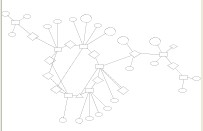
\includegraphics[width=8cm]{images/sisBccKompakt.png}
		\caption{Datenmodell Schulinformationssystem mit BCC Kompakt}
		\label{bccKompaktSis}
	\end{center}
\end{figure}



\newpage

\section{GraphML}
\prc

\textit{GraphML} ist ein einfaches Dateiformat das für die Erstellung von Graphen genutzt werden kann. Dabei handelt es sich um eine Grundlage die die strukturellen Eigenschaften eines Graphen beschreiben kann. Die unterstützten Grundlagen laut \cite{graphml} sind:

\begin{itemize}
	\item gerichtete, ungerichtete und gemischte Graphen
	\item Hypergraphen
	\item hierarchische Graphen
	\item Referenzen auf externe Daten
	\item Applikationsspezifische Attribut-Daten und
	\item light-weight Parser
\end{itemize}

\noindent
Das Dateiformat basiert auf XML was es einfach macht damit Graphen zu generieren, archivieren und entwickeln.

\subsection{Hintergrund}

Die Entwicklung von GraphML während eines Workshops auf der Graph Drawing Symposium im Jahre 2000 in Williamsburg. Ein erster Ansatz für das Endergebnis wurde auf der Graph Drawing Symposium, 2001 in Wien vorgestellt \footfullcite{graphml}.
\\

\noindent
Seither wurden laufend Erweiterungen erstellt und auch Anwendungen die auf diesem Dateiformat aufbauen. Eine dieser Anwendungen ist das in Kapitel \ref{yed} beschriebene Programm yEd. Die folgenden Kapitel beziehen sich auf das modifizierte GraphML Format für yEd.

\subsection{Grundelemente und Aufbau}

Aufgrund der Eigenschaft, dass es sich bei GraphML um ein XML-Dokument handelt ist der Aufbau übersichtlich und man kann mit nur vier Elementen einen ganzen Graphen beschreiben \footfullcite{graphmltutorial}. Zu diesen vier Elementen gehören:

\begin{itemize}
	\item Das \textit{graphml}-Element, dass das \textit{root}-Element des Graphen bildet.
	\item Das \textit{graph}-Element, dass den Graphen kennzeichnet.
	\item Das \textit{node}-Element, dass einen Knoten des Graphen widerspiegelt.
	\item Das \textit{edge}-Element, dass die Kanten zwischen den Knoten repräsentiert.
	\\
\end{itemize}

\noindent
Innerhalb des \textit{graph}-Elements sind die Elemente für die Knoten und Kanten des Graphen angesiedelt. Hierbei muss aber nicht auf die Reihenfolge der Elemente geachtet werden.

\subsection{Generierung der Datei und Aufbau}

Um einen GraphML-Datei für yEd zu erstellen bietet yWorks, die Entwickungsfirma der Applikation, eine APi mit dem Namen yFiles an. Diese kann man aber nur für Java, JavaFX, .NET, WPF und HTML verwenden. Weil wir als Diplomarbeitsteam uns dazu entschieden haben \textit{Pyhton} als Programmiersprache zu verwenden stieß man hierbei schon auf die ersten Probleme. 
\\

\noindent
Jedoch konnte durch den Aufbau der Datei als XML und durch reverse Engineering, der Graph in Form von XML als Text in eine Datei geschrieben werden. Dementsprechend wurde ein Konvertierer entwickelt der die Informationen der XERML-Datei sinngemäß in eine GraphML-Datei umwandelt, damit hinterher ein vollständiges ER-Diagramm erstellt wird.

\subsubsection{Initiierung der Datei}

Damit die Datei von yEd korrekt gelesen werden kann müssen auch die entsprechenden \textit{Namensräume} für das XML gesetzt werden. Zudem werden von yEd in der GraphML-Datei \textit{key-Elemente} verwendet um den Knoten und Kanten innerhalb des Graphen den richtigen Typ zuweisen zu können. Bei der Initiierung wird zudem noch das Root-Element der GraphML-Datei erstellt. Hierbei ist anzugeben ob es sich bei dem Graphen um einen gerichteten, ungerichteten oder gemischten Graphen handelt. Für den gewählten Ansatz wird ein gerichteter Graph erstellt, weil dies auch die gewählte Einstellung von yEd ist bei der Erstellung eines ER-Diagramms, wie sich durch reverse Engineering herausgestellt hat.
\\

\noindent
Der XML-Code bis nach dem öffnen des \textit{graph}-Elements sieht also wie folgt aus:

\begin{lstlisting}[language=XML, label={xmlHeader}, caption={Header der GraphML-Datei mit nötigen Namensräumen}]
<?xml version="1.0" encoding="UTF-8" standalone="no"?>
<graphml xmlns="http://graphml.graphdrawing.org/xmlns"
	xmlns:java="http://www.yworks.com/xml/yfiles-common/1.0/java"
	xmlns:sys="http://www.yworks.com/xml/yfiles-common/markup/primitives/2.0" 
	xmlns:x="http://www.yworks.com/xml/yfiles-common/markup/2.0"
	xmlns:xsi="http://www.w3.org/2001/XMLSchema-instance"
	xmlns:y="http://www.yworks.com/xml/graphml"
	xmlns:yed="http://www.yworks.com/xml/yed/3"
	xsi:schemaLocation="http://graphml.graphdrawing.org/xmlns
	http://www.yworks.com/xml/schema/graphml/1.1/ygraphml.xsd">
<key for="node" id="d1" yfiles.type="nodegraphics"/>
<key for="edge" id="d2" yfiles.type="edgegraphics"/>
<graph edgedefault="directed" id="G">
\end{lstlisting}

\subsubsection{Erstellung der Knoten und Kanten}
\prc

Die Informationen für die Erstellung der Knoten und Kanten werden aus einem ,,\textit{etree}'' ausgelesen der zuvor mithilfe der XERML-Datei des Benutzers erstellt wird. Beim Konverter werden diese Informationen dann analysiert und in ein entsprechendes Format für die GraphML Datei umgewandelt.

\subsubsubsection{Knoten}

\noindent
Beim Schreiben des XML-Codes für die Knoten wird ein Element für einen Knoten mit einer \textit{ID} als Attribut angelegt. Mithilfe dieser ID können später die Kanten zwischen den Knoten gezeichnet werden. Innerhalb des Knotenelements sind ein \textit{data-Element}. Diese zwei XML-Elemente gehören zu den grundlegenden GraphML-Elementen. Die spezifische Information über dem Knoten, den man am Ende im ER-Diagramm sieht, steht im \textit{GenericNode} der ein Kindelement von dem data-Element ist. 
\\

\noindent
In der folgenden Strukturbeschreibung sieht man wie ein Knoten in GraphML für die Verwendung mit yEd aufgebaut ist. Man beachte jedoch, dass Attribute mit Standardwerten beim Element \textit{NodeLable} weggelassen wurden, weil diese ohnehin nicht  beeinflusst werden.

\begin{verbatim}
Element: node
|
+-- Attribut: id
+-- Element: data
    |
    +-- Attribut: key
    +-- Element: y:GenericNode
        |
        +-- Attribut: configuration
        +-- Element: y:Geometry
            |
            +-- Attribut: heigth
            +-- Attribut: width
            +-- Attribut: x
            +-- Attribut: y
        +-- Element: y:Fill
            |
            +-- Attribut: hasColor
            +-- Attribut: color
            +-- Attribut: transparent
        +-- Element: y:NodeLable
        +-- Element: y:StyleProperties
            |
            +-- Element: y:Property
                |
                +-- Attribut: class
                +-- Attribut: name
                +-- Attribut: value
\end{verbatim}
\prc

\noindent
Diese Struktur ist aber nicht immer gleich. Zum Beispiel wird das Element \textit{StyleProperties} nur als Kindelement von Node angeführt, wenn es sich bei dem Knoten um einen schwachen Entitytypen handelt. Weiteres ist das Attribut \textit{color} nur dann gesetzt, wenn der Benutzer sein ER-Diagramm farbig haben möchte. 
\\

\noindent
Im nachfolgenden XML-Beispiel sieht man wie der Entitytyp ,,Person'' aus dem Datenmodell Schulinformationssystem aussieht, wenn dieser nicht färbig dargestellt wird:

\begin{lstlisting}[language=XML, caption=Entitytyp Person dargestellt in GraphML, label={xmlTypen}]
<node id="n0">
	<data key="d1">
		<y:GenericNode configuration="com.yworks.entityRelationship.small_entity">
			<y:Geometry height="50.0" width="90.0" x="285.0" y="135.0"/>
			<y:Fill hasColor="false" transparent="false"/>
			<y:NodeLabel alignment="center" autoSizePolicy="content"
				fontFamily="Dialog" fontSize="12" fontStyle="plain"
				height="17.96875" horizontalTextPosition="center"
				iconTextGap="4" modelName="internal" modelPosition="c"
				textColor="#000000" verticalTextPosition="bottom"
				visible="true">Person</y:NodeLabel>
		</y:GenericNode>
	</data>
</node>
\end{lstlisting} 

\noindent
Wie man ebenfalls anhand des Beispieles sehen kann, wird in Zeile 3 durch das Attribut \textit{configuration} der Typ des Knoten festgelegt. Bei der Erstellung eines ER-Diagramms werden im gegebenen Sachzusammenhang zwischen 3 Typen unterschieden:
\\

\begin{itemize}
	\item \begin{verbatim}small_entity\end{verbatim}
	- für einen Entitytyp
	\item \begin{verbatim}relationship\end{verbatim}
	- für einen Beziehungstyp
	\item \begin{verbatim}attribute\end{verbatim}
	- für ein Attribut
	\\
\end{itemize}

\noindent
Abhängig vom Typ der an jener Stelle angeführt ist, wählt yEd eine andere Form um den Knoten darzustellen. Wie der Knoten aus dem Beispiel aussieht, kann man in Abbildung \ref{entityPerson} sehen.

\begin{figure}[!h]
	\begin{center}
		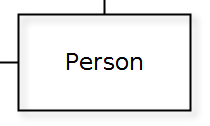
\includegraphics[width=6cm]{images/entityPerson.png}
		\caption{Entitytyp Person dargestellt in yEd}
		\label{entityPerson}
	\end{center}
\end{figure}

\subsubsubsection{Kanten}
\prc

\noindent
Die Kanten werden in einer GraphML-Datei über ein \textit{edge-Element} beschrieben. Dieses Elemen,t enthält genauso wie auch schon das node-Element eine ID, zusätzlich bekommt es jedoch die Attribute \textit{source} und \textit{target} die als Werte jene IDs der Knoten erhalten, die diese Kante zusammenhalten soll.
\\

\noindent
Wie auch schon bei den Knoten werden in der folgenden Strukturbeschreibung für die Kanten in einer GraphML-Datei all jene Attribute und Elemente beim Element \textit{EdgeLable} weggelassen, die mit Standardwerten initiiert sind.

\begin{verbatim}
Element: edge
|
+-- Attribut: id
+-- Attribut: source
+-- Attribut: target
+-- Element: data
    |
    +-- Attribut: key
    +-- Element: y:PolyLineEdge
        |
        +-- Element: y:LineStyle
            |
            +-- Attribut: color
            +-- Attribut: type
            +-- Attribut: width
        +-- Element: y:Arrows
            |
            +-- Attribut: source
            +-- Attribut: target
        +-- Element: y:EdgeLable

\end{verbatim}

\noindent
Dadurch das der Benutzer von ERMTK sich bei der Generierung einer GraphML-Datei entscheiden kann ob er sein ER-Diagramm in der Crow-foot Notation oder in der (min,max)-Notation, fällt bei der Crow-foot Notation das Element EdgeLable weg.
\\

\noindent
Im folgendem XML-Beispiel sieht man die Kante die den Entitytypen ,,Person'' mit dem Beziehungstypen ,,ist Elternteil von'' verbindet:

\begin{lstlisting}[language=XML, caption=Kante zwischen einem Entitytypen und einem Beziehungstypen, label={xmlKanten}]
<edge id="e26" source="n0" target="n19">
	<data key="d2">
		<y:PolyLineEdge>
			<y:LineStyle color="#000000" type="line" width="1.0"/>
			<y:Arrows source="none" target="none"/>
			<y:EdgeLabel alignment="center" configuration="AutoFlippingLabel"
				distance="2.0" fontFamily="Dialog" fontSize="12"
				fontStyle="plain" hasBackgroundColor="false"
				hasLineColor="false" height="17.96875"
				horizontalTextPosition="center" iconTextGap="4"
				modelName="custom" preferredPlacement="source_right"
				ratio="0.5" textColor="#000000" verticalTextPosition="bottom"
				visible="true" width="90.3203125" x="-15.16015625"
				xml:space="preserve" y="-22.94091796875003">
				(0,n)
				<y:LabelModel>
					<y:SmartEdgeLabelModel autoRotationEnabled="false" defaultAngle="0.0"
						defaultDistance="10.0"/>
				</y:LabelModel>
				<y:ModelParameter>
					<y:SmartEdgeLabelModelParameter angle="0.0"
						distance="30.0" distanceToCenter="true" position="right" ratio="0.0" 
						segment="0"/>
				</y:ModelParameter>
			<y:PreferredPlacementDescriptor angle="0.0"
				angleOffsetOnRightSide="0" angleReference="absolute"
				angleRotationOnRightSide="co" distance="-1.0"
				placement="source" side="right"
				sideReference="relative_to_edge_flow"/>
			</y:EdgeLabel>
		</y:PolyLineEdge>
	</data>
</edge>
\end{lstlisting}

\noindent
Wie man in der 1. Ziele des Beispiels erkennen wird dort die Information gespeichert welche Knoten verbunden werden. Dies wird dann in yEd wie in der Abbildung \ref{yedKante} dargestellt.

\begin{figure}[!h]
	\begin{center}
		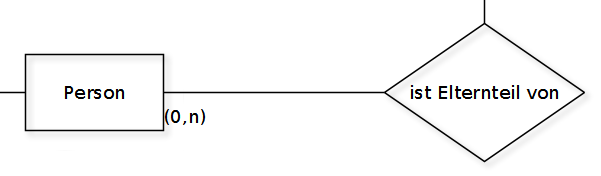
\includegraphics[width=10cm]{images/yedKante.png}
		\caption{Entitytyp Person dargestellt in yEd}
		\label{yedKante}
	\end{center}
\end{figure}

\subsection{Python-Code für die Generierung}

Um die GraphML-Datei für yEd zu erstellen, wurde die Klasse \textit{GraphmlConverter} geschrieben die den Inhalten der XERML-Datei in das richtige Format bringt und in eine Datei schreibt.
\\

\noindent
Zu Beginn wird die Datei, die später mit yEd geöffnet werden soll erstellt. Dazu wird der Parameter \textit{output} abgefragt, den der Benutzer angeben kann. Je nach Angaben des Benutzers wird die Datei an dem momentanen Pfad mit dem Namen \textit{output.graphml} erstellt an dem der Benutzer den Befehl ausgeführt hat oder er gibt einen Pfad mit Namen an, andem die Datei erstellt werden soll. Der Codeausschnitt \ref{createFile} behandelt diesen Fall:


\begin{lstlisting}[language=Python,label={createFile},caption={Codeausschnitt für die Erstellung der GraphML-Datei}]
try:
	if args.output is None:
		if os.path.exists("output.graphml"):
			os.remove("output.graphml")
		self.out = open("output.graphml", "w+")
	else:
		if os.path.exists(os.getcwd() + "/" + args.output):
			os.remove("./" + args.output)
		self.out = open(os.getcwd() + "/" + args.output, "w+")
	self.init_file()
except IOError:
	print(Fore.RED + "There was a Problem creating the file. Please try again" + Fore.RESET)
	return
\end{lstlisting}

\prc
\noindent
Wie man in Zeile 10 von \ref{createFile} sieht, wird dort die Funktion \textit{init\_file()} aufgerufen. In dieser Funktion wird die Datei soweit vorbereitet, dass der XML-Code für die Entity- und Beziehungstypen \ref{xmlTypen} und für die Kanten \ref{xmlKanten} hineingeschrieben werden kann. Der XML-Code der dabei hineingeschrieben wird ist in Listing \ref{xmlHeader} zu sehen.
\\

\noindent
Anschließend wird in einem XML-Baum der die Informationen aus der XERML-Datei enthält nach den Entity- und Beziehungstypen gesucht damit auch diese ihren Weg in die GraphML-Datei finden. Dieser Vorgang wird in dem Listing \ref{searchElements} vereinfacht dargestellt. Vereinfacht bedeuted in diesem Sinne, dass \textit{if}-Anweisungen, \textit{for}-Schleifen, und Definitionen von Variablen sowie deren Verwendung bei den Funktionsaufrufen weggelassen werden, damit die Logik des Codes im Vordergrund steht. Die komplette Darstellung des Codes kann man im Anhang finden.
\\

\begin{lstlisting}[language=Python, label={searchElements}, caption={Vereinfachter Code zum hizufügen der Entity- und Beziehungstypen}]
root = self._tree.getroot()
#------------------------------------------------------------------------------------------------------
for child in root:
	if child.tag == "ent":
		self.create_node()
		if args.attr:
			for attr in child:
				self.create_attribute()
#------------------------------------------------------------------------------------------------------
	elif child.tag == "rel":
		for part in child:
			if part.tag == "part":
				self.create_node()
#------------------------------------------------------------------------------------------------------
				if args.notation == "crowfoot":
					# Die folgende if-Anweisung wird betreten wenn ein fuer beide Kantenenden ein Knoten definiert ist
					if key_e != "" and key != "":
						self.create_edge()
					else:
						print(Fore.RED + "There was an entity missing for a relationship" + Fore.RESET)
				else:
					# Die folgende if-Anweisung wird betreten wenn ein fuer beide Kantenenden ein Knoten definiert ist
					if key_e != "" and key != "":
						self.create_chen_edge()
					else:
						print(Fore.RED + "There was an entity missing for a relationship" + Fore.RESET)
#------------------------------------------------------------------------------------------------------
			elif part.tag == "super":
				if not generalization_node:
					generalization_node = True
					self.create_generalization_node()
					# Die folgende if-Anweisung wird betreten wenn ein fuer beide Kantenenden ein Knoten definiert ist
					if key_e != "" and key != "":
						if args.notation == "chen":
							self.create_chen_edge()
						else:
							self.create_edge()
					else:
						print(Fore.RED + "There was an entity missing for a relationship" + Fore.RESET)
#------------------------------------------------------------------------------------------------------
			elif part.tag == "sub":
				# Die folgende if-Anweisung wird betreten wenn ein fuer beide Kantenenden ein Knoten definiert ist
				if key_e != "" and key != "":
					if args.notation == "chen":
						self.create_chen_edge()
					else:
						self.create_edge()
				else:
					print(Fore.RED + "There was an entity missing for a relationship" + Fore.RESET)
			elif part.tag == "attr" and args.attr:
				self.create_attribute()
\end{lstlisting}
\prc

\noindent
Nachdem der vereinfachte Codeabschnitt \ref{searchElements} abgeschlossen ist, wird die GraphML-Datei ordnungsgemäß mit der Funktion \textit{close\_file()} geschlossen. Als letzten Schritt wird dem Benutzer noch mitgeteilt, wo sich die GraphML-Datei befindet, damit dieser sein ER-Diagramm in yEd inspizieren kann.





\newpage

\newpage
\section{Graphviz}
\fib{}
\subsection{Allgemeines}

\noindent
Graphviz ist eine Open-Source Software mit der man Graphen darstellen kann.
Entwickelt wurde es von AT\&T und den Bell Labs, die es zum Ersten mal in den 1990er veröffentlichten. Die aktuellste Version von Graphviz ist die Verion 2.41 und wurde am 25.Dezember 2016 veröffentlicht. Graphviz ist dazu da aus strukturierten Daten gerichtete oder ungerichtete Graphen zu generieren. 
\footcite{graphviz_nodate}

\noindent
Außerdem wird Graphviz in Programmen verwendet wie in z.B.:
\begin{itemize}
	\item AsciiDoc
	\item PlantUML
	\item Trac
	\item Sphinx
\end{itemize}
\noindent
Wobei die letzten beiden Programme im laufe des Projekts verwendet wurden.

\noindent
In drei von vier Ausgabeformaten dieses Projekts kommt Graphviz zum Einsatz. In einem Ausgabeformat, um damit selbst die Modelle zu generieren und in den anderen zwei Ausgabeformaten, um an die Koordinaten zu kommen an denen die Elemente positioniert werden müssen.

\subsubsection{Ablauf des Programms}

\noindent
\lstset{language=Python}
\lstset{frame=lines}
\lstset{caption={Programmcode, um einen Graphen anzulegen}}
\lstset{label={create_graph}}
\lstset{basicstyle=\footnotesize}
\begin{lstlisting}

name = "erd"
set = False
for child in _root:
if child.tag == "title":
name = child.get("name")
set = True
if set:
break
_erd = Graph(name, filename=name, engine="sfdp")
self.create_erd(args, _erd, _root)

\end{lstlisting}
\noindent
Im Listing \ref{create_graph} sieht man wie ein leerer Graph, der nur einen Namen und eine Engine besitzt, erstellt wird. 
Die Variable ``set,, verhindert das mehrfache setzen vom Namen des Graphen. 

\noindent
Für die Darstellung eines Entity-Relationship Diagramms werden folgende Formen benötit:
\begin{itemize}
	\item Raute (einfach umrandet oder doppelt umrandet)
	\item Rechteck (einfach umrandet oder doppelt umrandet)
	\item Ellipse (einfach umrandet oder strichliert umrandet)
	\item Dreieck (schwarz ausgemahlt oder leer)
\end{itemize}


\begin{figure}[H]
	\begin{center}
		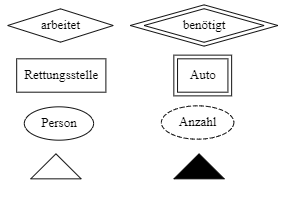
\includegraphics[width=16cm,height=10cm]{images/graphviz_formen.png}
		\caption{Formen in Graphviz}
		\label{dot}
	\end{center}
\end{figure}
\fib{}
\noindent
Diese Elemente werden dann mit Linien verbunden. Diese können im speziellen Fall einer totalen Vererbung auch als doppelte Linie vorkommen.
\lstset{language=Python}
\lstset{frame=lines}
\lstset{caption={Programmcode, um Entities zu erstellen}}
\lstset{label={create_ent}}
\lstset{basicstyle=\footnotesize}
\begin{lstlisting}

def create_ent(self, erd, name, weak):
if not weak:
erd.attr("node", shape="box", peripheries="1")
erd.node(name)
else:
erd.attr("node", shape="box", peripheries="2")
erd.node(name)

\end{lstlisting}
\noindent
Um einen Entity-Typen zu zeichnen muss vorher der Name des Entity-Typen und ob er abhängig oder nicht abhängig ist bekannt sein. Außerdem muss der Graph in dem das Element sich befindet mitgegeben werden. Wie man im Listing \ref{create_ent} sieht wird durch eine if-Verzweigung darüber entschieden ob ein Rechteck mit doppeltem Rand oder einfachem Rand erstellt wird. Dementsprechend werden die Eigenschaften von ``erd.attr,, mit dem Namen node angepasst.
\newpage
\fib{}
\noindent
\lstset{language=Python}
\lstset{frame=lines}
\lstset{caption={Programmcode, um Attribute zu erstellen}}
\lstset{label={create_attr}}
\lstset{basicstyle=\footnotesize}
\begin{lstlisting}

def create_attr(self, erd, name, prime, label):
if prime:
erd.attr("node", shape="ellipse", style="dashed", label=label)
erd.node(name)
else:
erd.attr("node", shape="ellipse", label=label)
erd.node(name)

\end{lstlisting}
\noindent
Bei dem Erstellen der Attribute muss zusätzlich zu Name und in welchem Graphen es sich befindet, auch bekannt sein ob es sich um einen Primär-Schlüssel handelt und zu welchem Entity-Typen das Attribut gehört. Der Parameter ``label,, ist der Name des Attributs und der Parameter ``name,, ist der Name von dem dazugehörigen Entity-Typen. Durch den Parameter ``prime,, wird in der if-Verzweigung, die man im Listing \ref{create_attr} sieht, ob es sich um einen Primär-Schlüssel handelt. Falls dem so ist wird die Ellipse mit strichliertem Rand erstellt.

\noindent
\lstset{language=Python}
\lstset{frame=lines}
\lstset{caption={Programmcode, um Beziehung zu erstellen}}
\lstset{label={create_rel}}
\lstset{basicstyle=\footnotesize}
\begin{lstlisting}

def create_rel(self, erd, name, weak, sup, disjoint):
if weak:
erd.attr("node", shape="diamond", peripheries="2")
erd.node(name)
elif sup:
if disjoint:
erd.attr("node", shape="triangle", color="black")
erd.node(name=name, style="filled")
else:
erd.attr("node", shape="triangle", color="white")
erd.node(name=name, style="filled")
else:
erd.attr("node", shape="diamond", peripheries="1")
erd.node(name)

\end{lstlisting}
\noindent
Für die Erstellung von den Beziehungen zwischen zwei Entity-Typen muss man angeben ob es sich um eine abhängige Beziehung handelt oder nicht, außerdem muss noch angegeben werden ob eine Vererbung vorliegt und wenn ja ob sie disjunkt oder nicht disjunkt ist. Wie man im Listing \ref{create_rel} sieht wird zunächst unterschieden, ob die Beziehung einer Vererbung angehört, einem abhängigen Entity-Typen angehört oder ob sie eine gewöhnliche Beziehung zwischen zwei Entity-Typen ist. Je nachdem wird dann entweder eine Raute oder ein Dreieck erstellt. Außerdem wird darüber entschieden ob das Dreieck schwarz gefüllt ist oder weiß ist. Der Beziehung ist zu diesem Zeitpunkt nicht bekannt mit welchen Linien sie mit welchen Entity-Typen verbunden wird.
\newpage
\fib{}
\noindent
\lstset{language=Python}
\lstset{frame=lines}
\lstset{caption={Programmcode, um Formen zu verbinden}}
\lstset{label={create_line}}
\lstset{basicstyle=\footnotesize}
\begin{lstlisting}

def create_edgeTotal(self, erd, ent1, ent2):
erd.edge(ent1, ent2, peripheries="2")

def create_edgeRel(self, erd, ent1, ent2, mini, maxi):
s = "(" + mini + ", " + maxi + ")"
erd.edge(ent1, ent2, label=s, peripheries="1")

def create_edge(self, erd, ent1, ent2):
erd.edge(ent1, ent2, peripheries="1")

\end{lstlisting}
\noindent
\begin{itemize}
	\item Um gewöhnliche Entity-Typen mit einem normalen Beziehungs-Typen zu verbinden wird die Funktion ``create edgeRel,, verwendet. Dabei werden die beiden Formen im Graphen mitgegeben, der Graph selbst und min und max werte des Beziehungs-Typen.
	\item Im Falle einer Vererbungen mit einer totalen Beziehung wird die Funktion ``create edgeTotal,, verwendet.  Dabei werden nur die beiden Formen im Graphen mitgegeben und der Graph selbst.
	\item Für jeden anderen Fall wird die Funktion ``create edge,, verwendet aber wird diese Funktion am häufigsten beim verbinden der Attribute  mit dem dazugehörigen Entity-Typen.
\end{itemize}

\noindent
\lstset{language=Python}
\lstset{frame=lines}
\lstset{caption={Programmcode, um Formen zu verbinden}}
\lstset{label={create_line}}
\lstset{basicstyle=\footnotesize}
\begin{lstlisting}

erd.render(format="pdf")
cwd = os.getcwd()
print("Your ERD is sucessfully created in:" + cwd)

\end{lstlisting}

\noindent
Nachdem der Graph und die Formen erstellt wurden und die Formen miteinander verbunden wurden. Wird das Dateiformat angegeben in welchem der Graph ausgegeben werden soll. Außerdem wird das Verzeichnis in dem die Datei gespeichert wird auf der Konsole ausgegeben.


\newpage
\subsection{Dateiformate}
\fib{}
\noindent
Graphviz bietet standardmäßig eine Vielzahl an verschiedenen Datei- oder Output-Formaten an.
Insgesamt sind es 55 verschiedene Formate und allein davon sind sechs Formate Variationen des ``dot,, Formats. Für dieses Projekt wurden hauptsächlich das PDF-Format genutzt. Das PIC-Code-Tool verwendete jedoch das ``pic-Format,, um die Koordinaten des Graphen mittels Graphviz zu ermitteln und an das Tool weiterzuleiten.
\footcite{noauthor_output_nodate}
Zu den gängigsten Datenformaten zählen:
\begin{itemize}
	\item dot
	\item bmp
	\item json
	\item pdf
	\item svg
	\item png
\end{itemize}

\subsubsection{dot-Format}
Die Ausgabe dieses Formats und der Formate gv, xdot, xdot1.2 und xdot1.4, erfolgt in dot-language. 
Darin stehen dann die Attribute für:
\begin{itemize}
	\item Begrenzungsrahmen
	\item Position
	\item Breite
	\item Höhe
	\item Labelpunkt
\end{itemize}
\noindent
Außerdem gibt es dann noch die Attribute ``rects,, und/oder ``vertices,, und noch weitere je nachdem welche Formen im Graphen angezeigt werden.

\subsubsubsection{xdot}
\noindent
``xdot,, steht für ``extended dot,, und ist einfach eine erweiterte Version von dot, die genauere Daten über den Graph zurück liefert als dot.
Kommentare für die Lesbarkeit und für das Verständnis kann man schreiben. Weiteres gibt es auch das Attribute ``xdotversion,, um Änderungen am Graphen zu erlauben. 

\subsubsubsection{xdot1.4}
\noindent
Mit``xdot1.4,, können Farbstrings lineare und radiale Farbverläufe codieren.
\begin{itemize}
	\item Lineare-Form:  '[' x0 y0 x1 y1 n [color-stop]+ ']'
	\item Radiale-Form:  '(' x0 y0 r0 x1 y1 r1 n [color-stop]+ ')' 
\end{itemize}
\noindent
Die Zahl n gibt an wie viele Color-stop es gibt. 
Wenn eine Form keine Farbe besitzt kann zu ihr auch keine Verbindung erstellt werden, auch wenn sie theoretisch existiert.


\newpage
\fib{}
\subsubsection{json}
\noindent
Dateiformate die JSON als ausgabe haben:
\begin{itemize}
	\item json
	\item json0
	\item dot json
	\item xdot json
\end{itemize}
\noindent
Bei Verwendung des Formats ``json,, bekommt man das selbe Ergebniss wie bei dem Format ``-Txdot,, nur als JSON anstelle einer Datei in DOT language. Genauso verhält es sich auch bei ``json0,, und ``-Tdot,,. Die Formate ``dot json,, und ``xdot json,, sind ``json0,, und ``json,, ähnlich. Jedoch verwenden diese zwei Formate nur die Input Daten und somit ist bei ihnen kein Layout durch einen bestimmten Algorithmus vorgegeben, dadurch enthalten diese Formate nur die Information über die Elemente selber.
Die daraus entstehende JSON-Datei kann wie folgt aufgebaut sein wie im Listing \ref{json}.

\noindent
\lstset{language=python}
\lstset{frame=lines}
\lstset{caption={Beispiel für eine JSON Datei von Graphviz}}
\lstset{label={json}}
\lstset{basicstyle=\footnotesize}
\begin{lstlisting}

{
"nodes": [
{
"id": "n0",
"label": "A node",
"x": 0,
"y": 0,
"size": 3
},
{
"id": "n1",
"label": "Another node",
"x": 3,
"y": 1,
"size": 2
},
],
"edges": [
{
"id": "e0",
"source": "n0",
"target": "n1"
},
{
"id": "e2",
"source": "n1",
"target": "n0"
}
]
}

\end{lstlisting}

\subsubsection{pdf}
\noindent
Das Format ``pdf,, erstellt ein PDF-Dokument.
Falls man Anker benutzen möchte sollte man als alternative das Format ``ps2,, benutzen, da das mit diesem möglich ist und dem Format ``pdf,, ähnelt.

\subsubsection{plain-ext}
\fib{}
Die Formate ``plain,, und ``plan-ext,, geben ein Text-Dokument aus dieses besteht aus vier verschiedenen Arten von Zeilen:
\begin{itemize}
	\item graph
	\item node
	\item edge
	\item stop
\end{itemize}
\noindent
Die ``stop,, Zeile markiert das Ende eines Graphen. Die Ausgabe besteht aus einer Zeile für den Graphen, mehreren Zeilen für Elemente, pro Element keine bis mehrere Zeilen für die Verbindungen und am Ende befindet sich ein Stop.

\subsubsubsection{graph}
\noindent
Die ``graph,, Zeile gibt die Breite sowie die Höhe des Graphen mit den Attributen ``height,, und ``width,, an. Wenn der Graph skaliert werden muss gibt es ein Attribute ``scale,,. Dieses Attribute gibt an in welchem Verhältnis der Graph skaliert werden muss. Außerdem sind alle Werte nicht skaliert was bedeutet, wenn der Wert des Attributes ``scale,, nicht 1.0 ist muss jede Zahl damit multipliziert werden. Standardmäßig ist der Koordinatenursprung in der linken unteren Ecke.

\subsubsubsection{node}
\noindent
Die ``node,, Zeilen besitzt die Attribute ``name,, welches dem Element seinen Namen verleiht, ein ``x,, und ein ``y,, Attribute welche die Position des Elements festlegen. Außerdem wird die Breite sowie die Höhe des Element, wie bei dem ``graph,, Statement mit den Attributen ``height,, und ``width,, angegeben. Außerdem verfügt es auch noch über die Attribute ``label,,, ``style,,, ``shape,,, ``color,, und ``fillcolor,,. Wenn das ``style,, Attribute leer ist, ist der Rahmen des Elements Standardmäßig solide.

\subsubsubsection{edge}
\noindent
Die zwei wichtigsten Attribute der ``edge,, Zeile sind ``tail,, und ``head,,, diese geben die zwei Namen der zu verbindenden Elemente an.

\subsubsection{png}
\noindent
Das ``png,, Format ist eines der unpraktischsten dafür einfachsten Formate da es lediglich ein Bild zurück liefert.
Jedoch kann man bei diesem Format einstellen ob das Bild mit Antialiasing generiert werden soll oder ohne. Außerdem kann man auch noch angeben ob es mit ``Indexed color,, oder mit ``True color,, generiert werden soll. 

\newpage
\subsection{Engines}
\fib{}
\noindent
Die sogenannten Engines in Graphviz geben an mit welchem Verfahren die Koordinaten der Elemente berechnet werden. Das kann von großem Vorteil sein wenn man bestimmte Ergebnisse erzielen will.
\footcite{noauthor_documentation_nodate}

\subsubsection{dot}

\noindent
dot ist in erster Linie dafür gedacht Strukturen hierarchisch abzubilden. Das bedeutet das dabei alle Kanten in etwa die selbe Richtung verlaufen, meistens von oben nach unten oder von links nach rechts. Durch diese Anordnung der Elemente kommt es selten zu Kanten Überschneidungen da sie auch in der Regel eher kurz gehalten werden.
Daher wird man eher dot verwenden wenn man weiß, dass die Kanten eine Richtung besitzen.

\begin{figure}[H]
	\begin{center}
		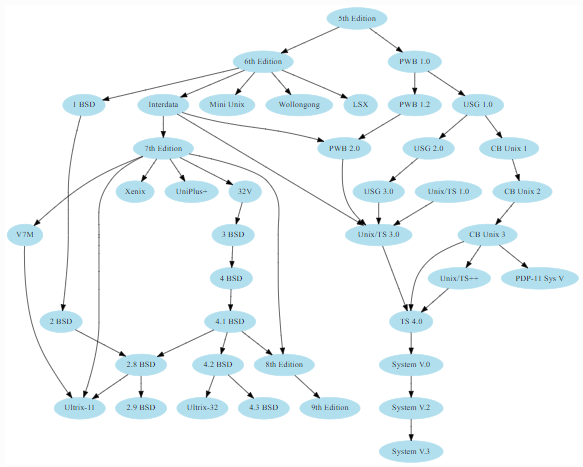
\includegraphics[width=16cm, height=10cm]{images/dot.png}
		\caption{Typischer dot Graph}
		\label{dot}
	\end{center}
\end{figure}
\footcite{noauthor_graphics_nodate}
\newpage
\noindent
\subsubsection{neato}
\fib{}
\noindent
neato benutzt das sogenannte ``spring model,, Layout. Neato benutzt den Kamada-Kawai-Algorithmus und ist eher dafür gedacht kleinere Graphen(um die 100 Knoten) darzustellen. Man benutzt Neato dann wenn man nichts außer der Größe des Graphen kennt. Neato führt einen Vorgang durch, beim generieren des Graphen, der äquivalent zu Multi-Dimensionaler Skalierung ist.
\footcite{north_drawing_2004}
\begin{figure}[H]
	\begin{center}
		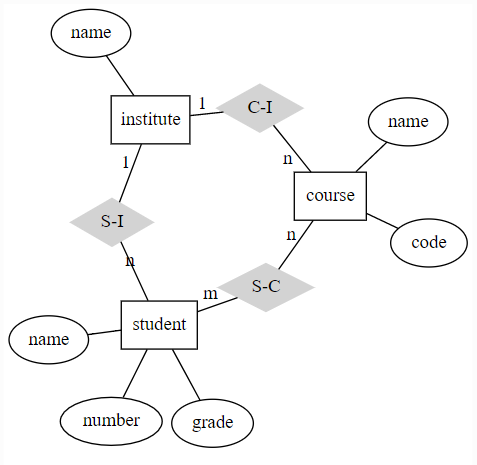
\includegraphics[width=14cm, height=8cm]{images/neato.png}
		\caption{Typischer neato Graph}
		\label{neato}
	\end{center}
\end{figure}

\noindent
\subsubsection{fdp}

\noindent
fdp benutzt genau wie neato auch das ''spring model,, Layout. Jedoch wendet es ein anderes Verfahren an.

\subsubsection{sfdp}

\noindent
sfdp benutzt genau wie fdp und neato auch das ''spring model,, Layout. Außerdem ist sdfp eine multiscale Variante von fdp mit der man sehr große Graphen darstellen kann.
\footcite{noauthor_performance_nodate}
\begin{figure}[H]
	\begin{center}
		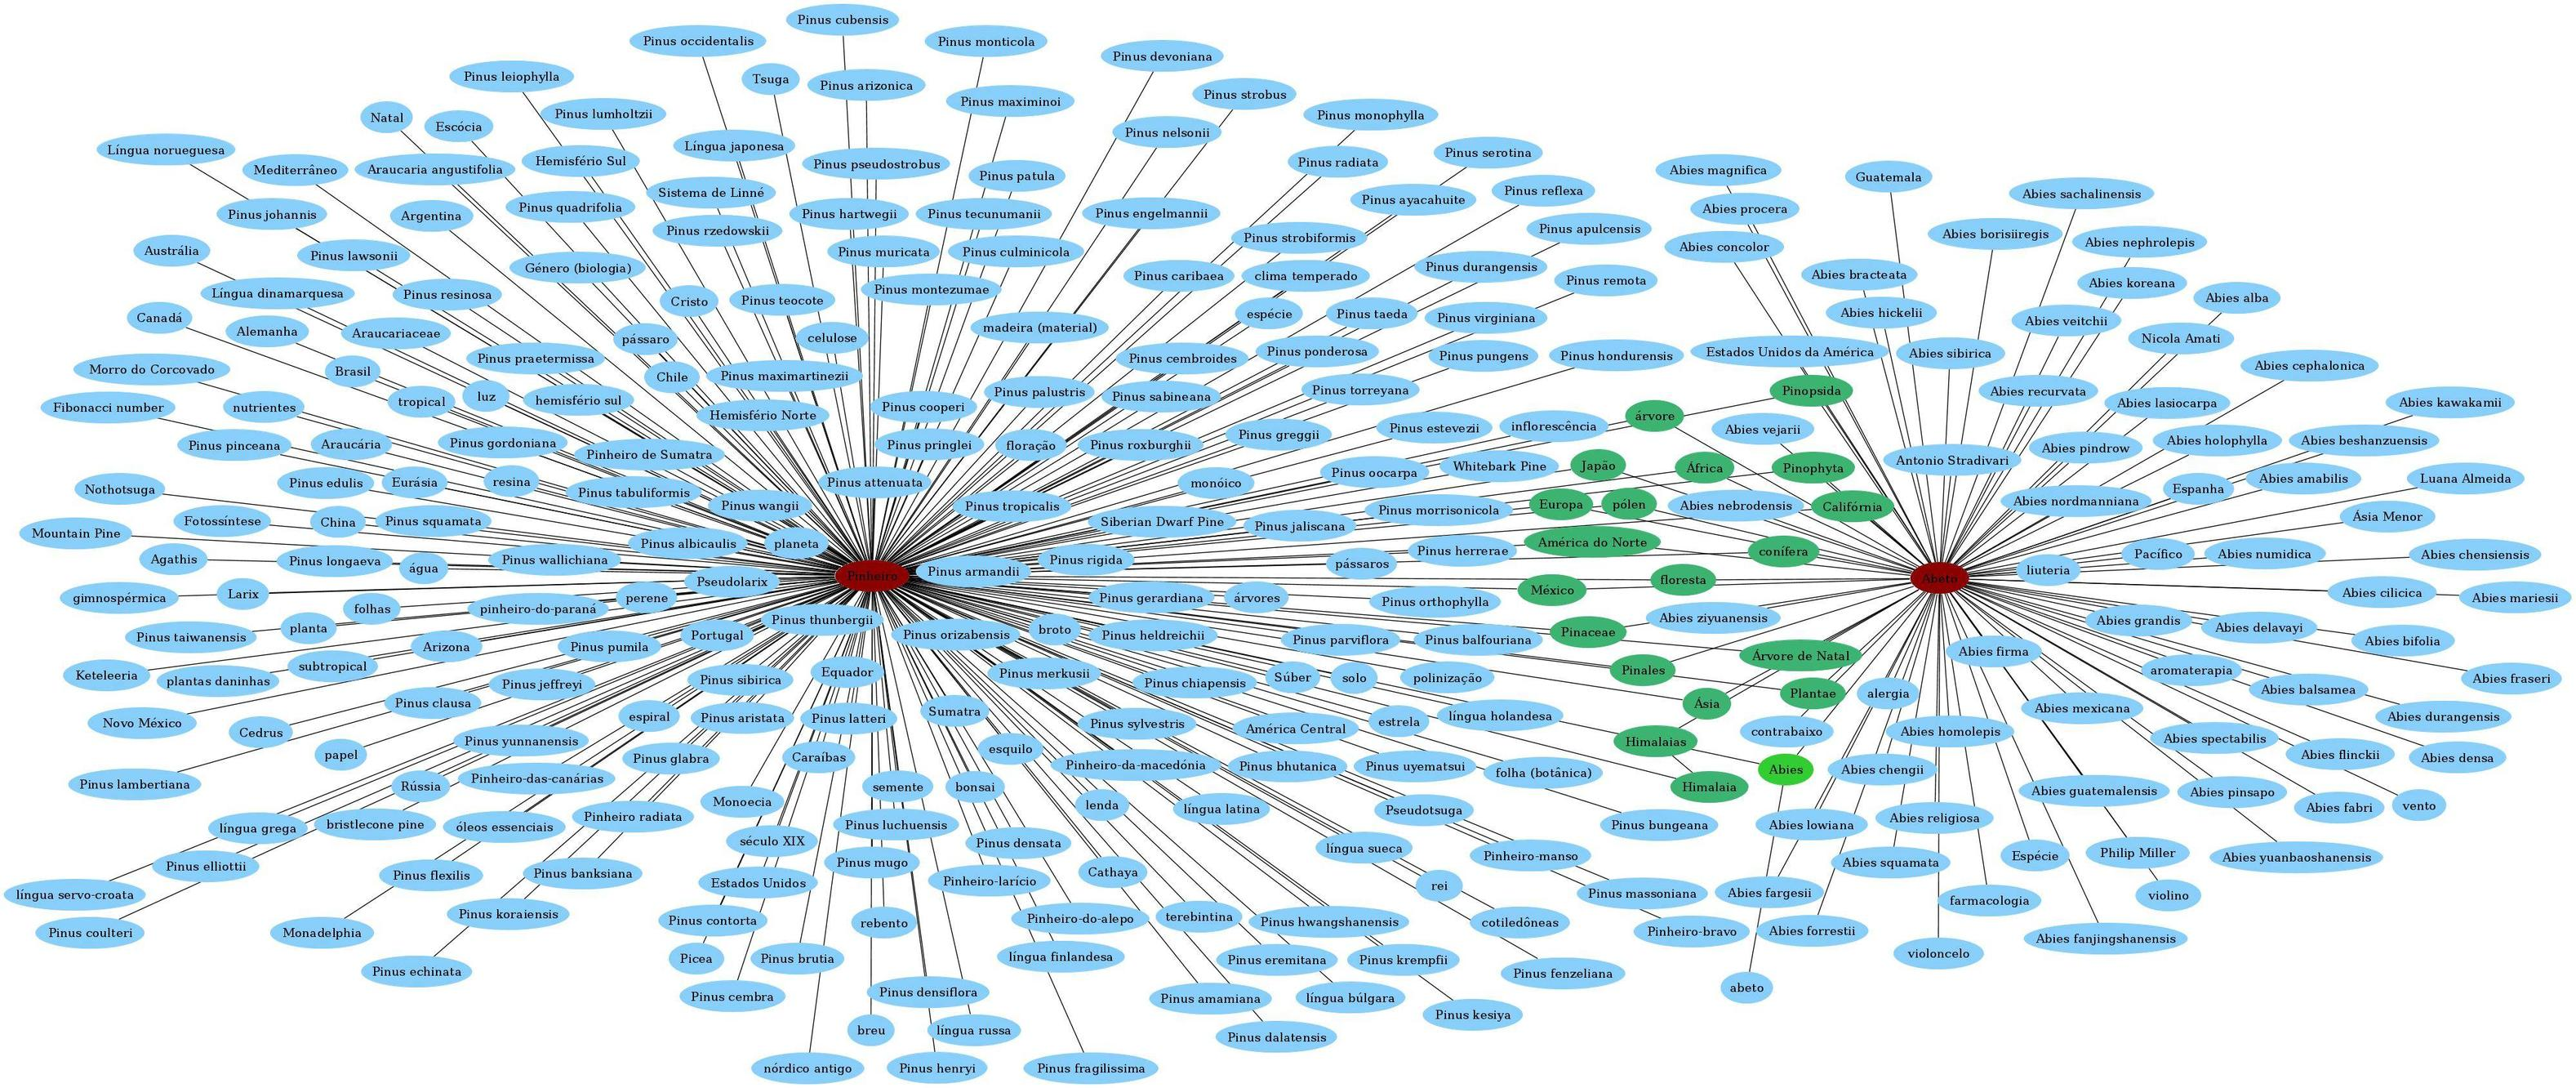
\includegraphics[width=14cm, height=8cm]{images/sfdp.jpg}
		\caption{Typischer sfdp Graph}
		\label{sfdp}
	\end{center}
\end{figure}

\noindent
\subsubsection{circo}
\fib{}
\noindent
circo erstellt ein circuläres Layout nach Six und Tollis 99, Kauffman und Wiese 02. Dieses Verhalten verlieh ihm auch seinen Namen. Diese Art von Graphen Generierung ist dazu geeignet Zyklische Strukturen, wie man sie meist bei Telekomunikations-Netzwerken vorfindet, darzustellen.

\begin{figure}[H]
	\begin{center}
		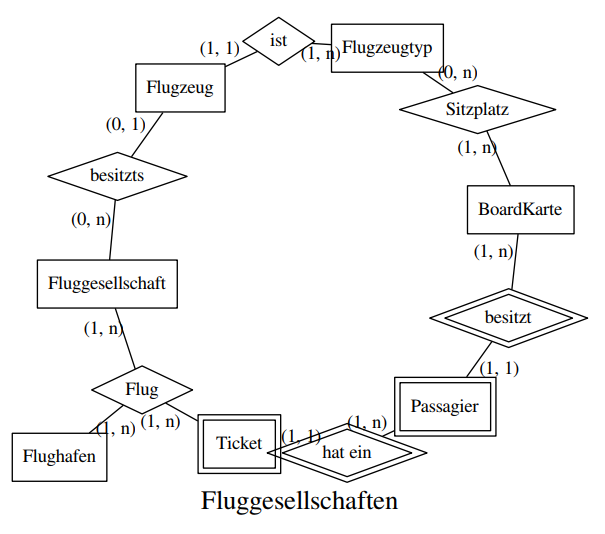
\includegraphics[width=14cm, height=8cm]{images/circo.png}
		\caption{Typischer circo Graph}
		\label{circo}
	\end{center}
\end{figure}

\noindent
\subsubsection{twopi}
\fib{}
\noindent
twopi erstellt ein radiales Layout nach Graham Wills 97. Dabei werden die Knoten auf konzentrischen Kreisen, abhängig von der Distanz zu einem Wurzel Knoten, platziert.

\begin{figure}[H]
	\begin{center}
		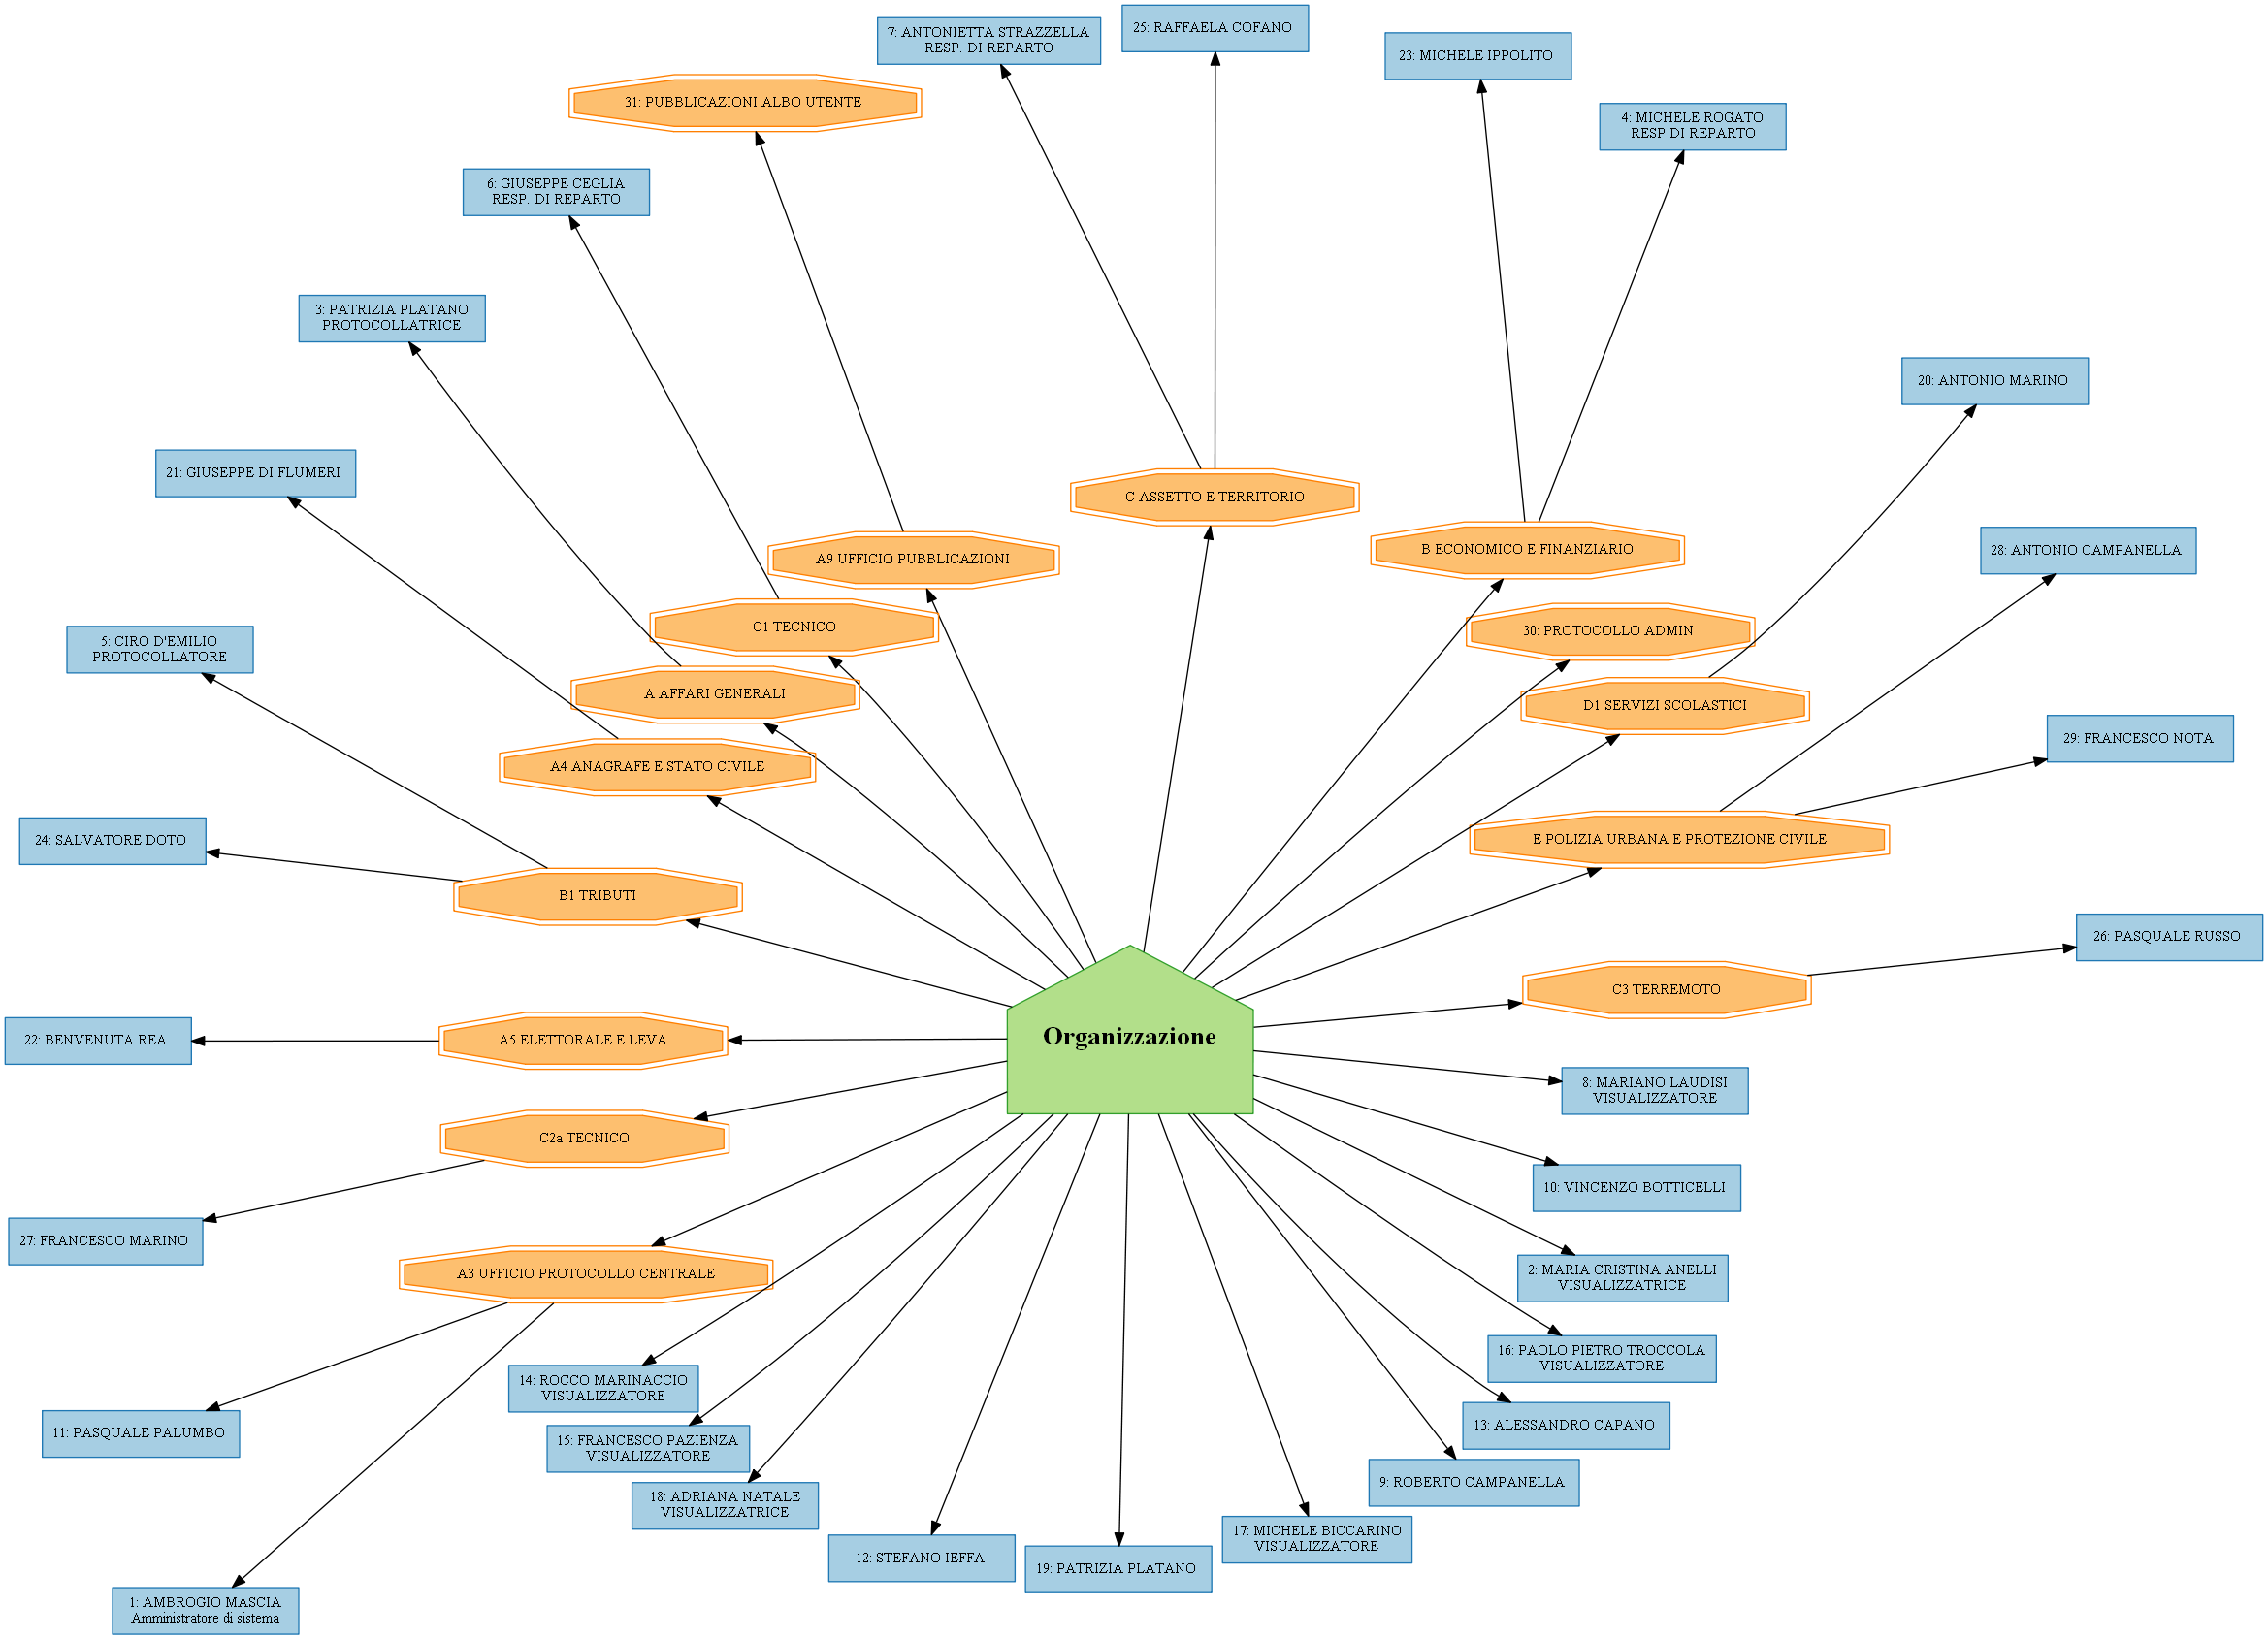
\includegraphics[width=14cm, height=6cm]{images/twopi.png}
		\caption{Typischer twopi Graph}
		\label{twopi}
	\end{center}
\end{figure}

\subsection{Vor- und Nachteile von Graphviz}
\subsubsection{Engines}
\subsubsubsection{Vorteile}
\noindent
Durch sechs verschiedene Engines kann man eine Vielzahl an verschiedenen Graphen erstellen. Wenn man genug über seinen Graphen in Erfahrung gebracht hat kann man die eine Engine die für seinen Graphen am besten passt auswählen und somit ein ideales Ergebnis erzielen.

\subsubsubsection{Nachteile}
\noindent
\begin{itemize}
	\item Jedoch der große Nachteil von Engines ist das man gebunden ist an sie. Man kann Beispielsweise nicht festlegen wo ein bestimmtes Element positioniert werden soll.
	\item  Außerdem kann man nicht bestimmen welche Größe die einzelnen Elemente haben sollen, da sie sich, je nach ihrem Inhalt, dynamisch anpassen.
\end{itemize}

\subsubsection{Formen}
\subsubsubsection{Vorteile}
\noindent
Es existiert eine Vielzahl an Formen und Linien, wodurch einem Freiheit bei der Modellierung ermöglicht wird.

\subsubsubsection{Nachteile}
\noindent
Ein Nachteil ist das man in seiner Freiheit eingeschränkt ist.
\begin{itemize}
	\item Will man eine neue Form festlegen, geht das schlicht und einfach nicht.
	\item Will man Text in einem Element unterstrichen haben, geht auch dies nicht.
	\item Beim modellieren hat man die freie Auswahl über schon vorhandenen Formen, jedoch um eigene Formen dann selbst zu erstellen bedarf es viel Arbeit und selbst dann ist das Ergebnis nicht zufrieden stellend und nicht immer das selbe.
	\item Ein anderer Nachteil ist, dass man wenn man ein Element verändert z.B.: einen anderen Rahmen gibt, dann wird das als neuer Standard angenommen und man muss, wenn man einen Sonderfall behandelt der selten vorkommt, jedes mal wieder den alten Standard festlegen.
\end{itemize}


\subsubsection{Dateiformate}
\subsubsubsection{Vorteile}
\noindent
Manche Dateiformate, wie z.B.: JSON, bieten einem die Möglichkeit nur auf die Informationen eines Graphen zuzugreifen die man auch wirklich benötigt. Das ist praktisch für Fälle wobei Graphviz nicht zur Darstellung verwendet wird sondern nur um das Layout festzulegen. 

\subsection{Vergleich von dot und neato}
\fib{}
\noindent
Die dot Engine erstellt hierarchische Graphen und die neato Engine gerichtete Graphen.
In der Regel wird dot häufiger genutzt, jedoch ist neato für Entity-Relationship Diagramme weit aus besser geeignet.
\footcite{graphviz_neato}

\subsubsection{Weingut}

\begin{figure}[H]
	\begin{center}
		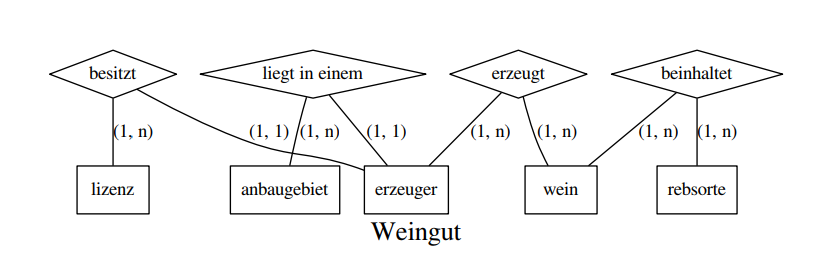
\includegraphics[width=16cm, height=8cm]{images/weingut_dot.png}
		\caption{Weingut mit der dot Engine}
		\label{wein_dot}
	\end{center}
\end{figure}

\noindent
Wie man an der oberen Abbildung \ref{wein_dot} sehen kann wäre dot für kleinere Graphen wie hier für dem Weingut durchaus denkbar. Solange Graphen nicht zu groß und nicht mehr als zwei Ebenen besitzen ist dot eine akzeptable Möglichkeit den Graph darzustellen.


\begin{figure}[H]
	\begin{center}
		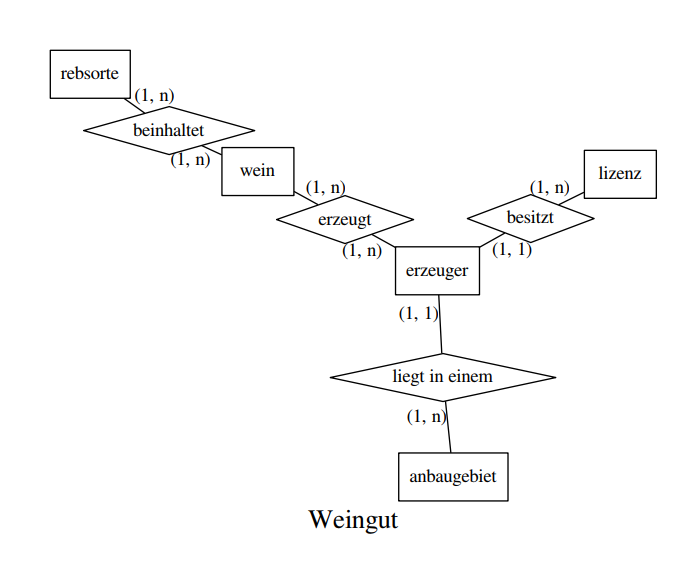
\includegraphics[width=16cm, height=8cm]{images/weingut_neato.png}
		\caption{Weingut mit der neato Engine}
		\label{wein_neato}
	\end{center}
\end{figure}

\noindent
Genau wie dot hat auch neato keinerlei Probleme mit kleinen Graphen wie dem Weingut.

\subsubsection{Rettungsstelle}

\begin{figure}[H]
	\begin{center}
		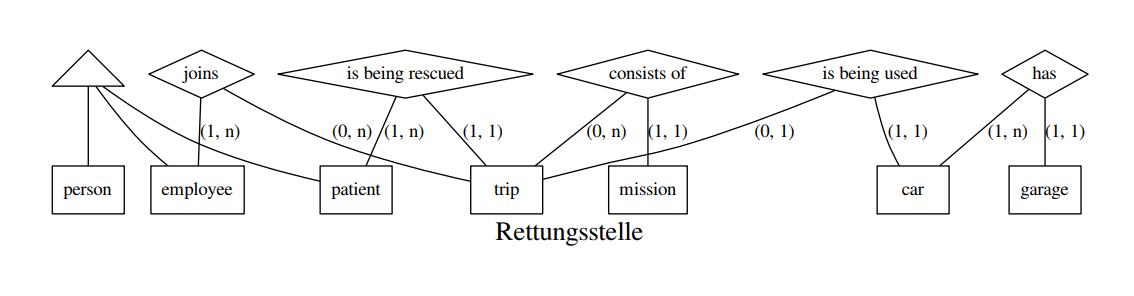
\includegraphics[width=16cm, height=8cm]{images/rettungsstelle_dot.png}
		\caption{Rettungsstelle mit der dot Engine}
		\label{rs_dot}
	\end{center}
\end{figure}
\fib{}
\noindent
Jedoch bei einem etwas größerem Graphen sieht man schon das dot zu breit wird und für Attribute keinen Spielraum mehr lassen würde.

\begin{figure}[H]
	\begin{center}
		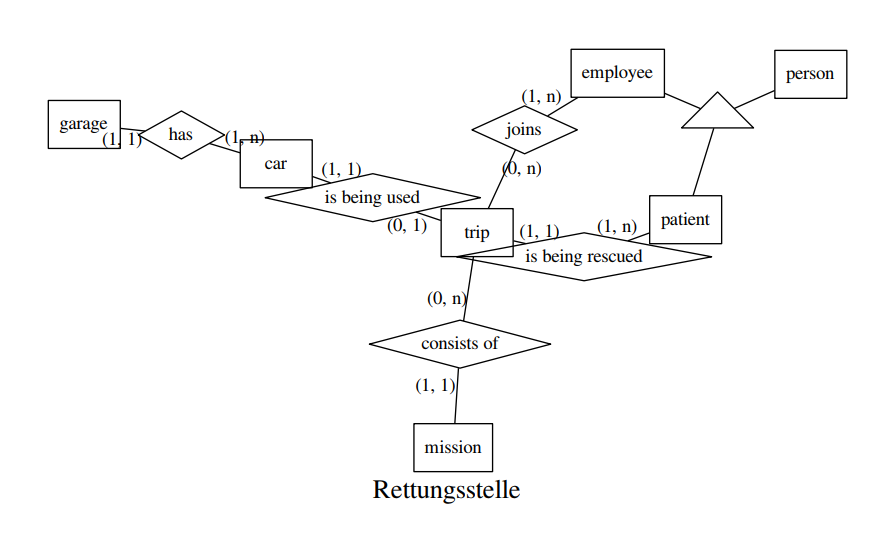
\includegraphics[width=16cm, height=8cm]{images/rettungsstelle_neato.png}
		\caption{Rettungsstelle mit der neato Engine}
		\label{rs_neato}
	\end{center}
\end{figure}

\noindent
Bei neato merkt man, wie hier bei der Rettungsstelle, dass noch Platz für Attribute wäre. Trotzdem merkt man das die Elemente immer näher aneinander rücken da der Graph für neato nicht die ideale größe besitzt.

\subsubsection{Wahl}
\fib{}
\noindent
Wenn man zwischen dot und neato wählen müsste sollte man vorher genaue Daten über den Graphen, den man generieren will, in Erfahrung bringen. In der Regel gilt beide eigenen sich für kleinere Graphen jedoch tut sich dot mit Attributen schwer und neato mit vielen Elementen. Bei vielen Elementen kann man aber auch sfdp benutzen da es neato ähnelt und auf größere Graphen ausgelegt ist.



\newpage

\section{LibreOffice Draw}

\subsection{Einführung in LibreOffice Draw}
\hon{}
Das vektorbasierte Grafikprogramm \textit{Draw} ist Teil des \textit{LibreOffice} Pakets und wurde von der \textit{The Document Foundation} entwickelt. Andere Bestandteile des \textit{LibreOffice} Pakets sind \textit{Writer, Calc, Impress, Base und Math}. \textit{Draw} bietet diverse Funktionalitäten um Skizzen, Poster, technische Zeichnungen, Flussdiagramme, verlustfrei skalierbare 2D-Vektorgrafiken mit 3D-Effekten, etc. zu erstellen. 
Der Funktionsumfang von \textit{Draw} gliedert sich in etwa zwischen den Grafikprogrammen \textit{Paint.NET} und \textit{GIMP} ein. Im Gegensatz zu \textit{Paint.NET} stehen mehrere vordefinierte 2D- und 3D-Formen zu Verfügung. Allerdings sind viele grafische Bearbeitungsfunktionen, die \textit{GIMP} zur Verfügung stellt, nicht enthalten. Alle \textit{LibreOffice} Programme sind auf den Plattformen \textit{Windows}, \textit{Linux} und \textit{macOS} verfügbar. Darüber hinaus wird die Webapp \textit{LibreOffice Online} angeboten, die auf einem Server installiert wird und über einen Webbrowser genutzt werden kann.
\textit{Draw} verwendet für die Speicherung und Darstellung der gezeichneten Objekte ein Koordinatensystem, wobei der Punkt [0,0] sich in der linken oberen Ecke der Seite befindet.
\footnotemark[30]
\footnotemark[31]

\subsection{Entwicklung}
\hon{}
Die Entwicklungsgeschichte des \textit{LibreOffice} Pakets beginnt mit dem Projekt \textit{StarDivision}, welches von dem Unternehmen \textit{StarOffice} initialisiert wurde. 1999 wurde das Unternehmen von \textit{Sun Microsystems} übernommen. Dieses gründete im darauffolgenden Jahr die Stiftung \textit{OpenOffice.org} mit dem Hauptziel die Weiterentwicklung der Software von Firmeneinflüssen zu bewahren. Im Januar 2010 wurde das Unternehmen \textit{Sun Microsystems} von \textit{Oracle} übernommen. Aufgrund einiger Meinungsverschiedenheiten und unzureichender finanzieller Unterstützung entschieden sich einige der führenden \textit{OpenOffice.org} Mitglieder im September des selben Jahres die gemeinnützige Stiftung \textit{The Document Foundation} zu gründen. Seitdem wird die Software unter dem Namen \textit{LibreOffice} vermarktet. Parallel dazu wird eine andere Version der Software von \textit{Apache}, die die Weiterentwicklung von \textit{Oracle} übernommen hat, unter dem Namen \textit{Apache OpenOffice} vermarktet. Bis auf die fehlende 64-Bit-Version bei \textit{Apache OpenOffice} und höhere Aktualisierungsintervalle bei \textit{LibreOffice} bestehen nur kleine Unterschiede zwischen den zwei verschiedenen Entwicklungszweigen.
Die Abbildung \ref{timeline} \footfullcite[][]{JavaLibreOfficeProgramming} zeigt den zeitlichen Verlauf grafisch.
\footfullcite[][]{LibreOfficeWikipedia}
\footfullcite[][]{LibreOffice}
\noindent
\begin{figure}
	\centering
	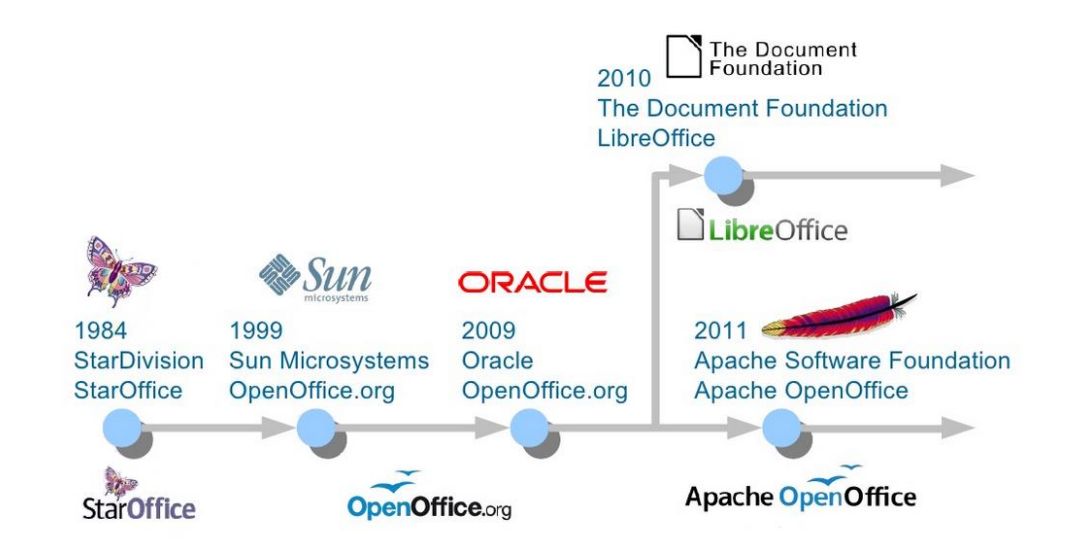
\includegraphics[width=13cm]{images/timeline.png}
	\caption{Timeline der Entwicklungsgeschichte}
	\label{timeline}
	
\end{figure}

\subsection{Generierungsvarianten}
\hon{}
Um ein \textit{Entity Relationship Diagramm} in \textit{LibreOffice Draw} automatisiert generieren zu können, bieten sich zwei Möglichkeiten an, die sich in der Komplexität und der Umsetzung sehr stark unterscheiden. Die erste der beiden Möglichkeiten ist der Zugriff über die zu Verfügung stehende \textit{API}. Die zweite Variante ist die Manipulation des Dateiformats.

\subsubsection{Generierung über die LibreOffice API}

\subsubsubsection{Allgemeines}
\hon{}
\\
\noindent
Um über die \textit{LibreOffice Programmierschnittstelle} (\textit{API}) auf ein \textit{Draw} Dokument zugreifen zu können benötigt man das \textit{LibreOffice Software Development Kit}. Dieses beinhaltet ein Set von Entwicklungswerkzeugen, Bibliotheken und Header-Dateien.
Auf der Website der \textit{LibreOffice} API befinden sich diverse Beispiele um die Funktionsweise und die Verwendung der \textit{API} zu demonstrieren. Die verschiedenen Beispiele unterscheiden sich in der verwendeten Programmiersprache und dem Zielprogramm. Als Programmiersprachen stehen \textit{Java, C++, Python, Basic} und das Objektsystem \textit{Object Linking and Embedding} zur Verfügung. Bei der genaueren Betrachtung zeigt sich, dass das einzige Beispiel, dass \textit{Draw} als Zielprogramm hat, in \textit{Java} geschrieben ist. 
\footfullcite[][]{LibreOfficeAPI}
\\
\hon{}
\\

\noindent
Um in ein \textit{Draw} Dokument zeichnen zu können, muss zuerst ein Dokument, eine Instanz der Klasse \verb|com.sun.star.frame.Desktop| mit einem Kontext der Klasse \verb|com.sun.star.uno.| \verb|XComponentContext| und einem \textit{Komponentenlader} mit der Instanz der Klasse \verb|com.sun.| \verb|star.frame.Desktop| angelegt werden. In der folgenden Grafik befindet sich ein Beispiel für jenen Code. (siehe Listing \ref{listing1})

\noindent
\hon{}
\lstset{language=Java}
\lstset{frame=lines}
\lstset{caption={Programmcode in Java, um ein leeres \textit{Draw} Dokument zu öffnen}}
\lstset{label={listing1}}
\lstset{basicstyle=\footnotesize}
\begin{lstlisting}

com.sun.star.frame.XComponentLoader xCLoader;
com.sun.star.lang.XComponent xComp = null;

try {
    com.sun.star.lang.XMultiComponentFactory xMCF = 
    xContext.getServiceManager();

    Object oDesktop = xMCF.createInstanceWithContext
    ("com.sun.star.frame.Desktop", xContext);

    xCLoader = UnoRuntime.queryInterface
    (com.sun.star.frame.XComponentLoader.class, oDesktop);
    com.sun.star.beans.PropertyValue szEmptyArgs[] = 
    new com.sun.star.beans.PropertyValue[0];
    String strDoc = "private:factory/sdraw";
    xComp = xCLoader.loadComponentFromURL
    (strDoc, "_blank", 0, szEmptyArgs);

} catch (java.lang.Exception e) {
    System.err.println(" Exception " + e);
    e.printStackTrace(System.err);
}
\end{lstlisting}
\footfullcite[][]{LibreOfficeAPI}

\noindent
\hon{}
\\
\noindent
Über einige weitere Schritte erhält man ein Objekt der Klasse \verb|xShapes|, in das man dann die zu zeichnenden Objekte hinzufügt. (siehe Listing \ref{listing2})
\noindent
\lstset{language=Java}
\lstset{frame=lines}
\lstset{caption={Programmcode in Java, um ein leeres \textit{Draw} Dokument zu öffnen}}
\lstset{label={listing2}}
\lstset{basicstyle=\footnotesize}
\begin{lstlisting}
xDrawDoc = openDraw(xContext);
try {
    System.out.println("getting Drawpage");
    com.sun.star.drawing.XDrawPagesSupplier xDPS = UnoRuntime
    .queryInterface(com.sun.star.drawing.
    XDrawPagesSupplier.class, xDrawDoc);
    com.sun.star.drawing.XDrawPages xDPn = xDPS.getDrawPages();
    com.sun.star.container.XIndexAccess xDPi = UnoRuntime
    .queryInterface(com.sun.star.container.XIndexAccess.class,
    xDPn);
    xDrawPage = UnoRuntime.queryInterface(com.sun.star.drawing.
    XDrawPage.class, xDPi.getByIndex(0));
} catch (java.lang.Exception e) {
    System.err.println("Couldn't create document" + e);
    e.printStackTrace(System.err);
}
\end{lstlisting}
\footnotemark[32]
\noindent
\\
\noindent
Mit dem in Listing \ref{listing1} und \ref{listing2} gezeigten Programmcode öffnet sich ein \textit{LibreOffice Draw} Dokument ohne Inhalt.

\noindent
\subsubsubsection{XERML-Daten Aufbereitung in Java}
\label{XERML-JAVA}
\hon{}

\noindent
Um die Daten aus der \textit{XERML}-Datei in ein für \textit{Java} interpretierbares Format zu bringen, wird der \textit{Java DOM Parser} verwendet. Die Daten werden immer in einer Liste des Datentyps \verb|ArrayList<String>| mit folgendem Aufbau gespeichert:
\begin{itemize}
	\item Für \textit{Entity-Typen} und zugehörige Attribute: Das erste Listenelement enthält den Namen des \textit{Entity-Typs}. Die folgenden Listenelemente enthalten die Namen der \textit{Attribute}.
	\item Für \textit{Beziehungstypen} und deren Teilnehmer: Das erste Listenelement enthält den Namen des \textit{Beziehungstyps}. Für jeden  Teilnehmer werden Listenelemente in folgender Reihenfolge hinzugefügt: Name des teilnehmenden \textit{Entity-Typs}, Minimalwert, Maximalwert.
	\item Für \textit{Beziehungsattribute}: Das erste Listenelement enthält den Namen des \textit{Beziehungstyps}. \textit{Beziehungsattribute} werden, falls vorhanden, dahinter angehängt.
	\item Für \textit{Primary-Keys}: Das erste Listenelement enthält den Namen des \textit{Entity-Typs}. Die darauffolgenden Listenelemente sind ein oder mehrere \textit{Primary-Keys}.
	\item Für \textit{Super-Sub-Beziehungstypen}: Das erste Listenelement enthält den Namen des \textit{Beziehungstyps}. Das zweite und dritte Listenelement enthalten den Wert des \textit{XERML-Attributs} \textit{total} an zweiter Stelle und den Wert des \textit{XERML-Attributs} \textit{disjunkt} an dritter Stelle. Dieser kann entweder \verb|true| oder \verb|false| sein. 
\end{itemize}


\noindent
\subsubsubsection{Darstellung der grafischen Elemente}
\hon{}

\noindent
Grundsätzlich folgt die Darstellung der verschiedenen grafischen Formen immer dem gleichen Schema. Zuerst wird ein Objekt, das die derzeitige Seite des Dokuments beinhaltet, angelegt. Dieses wird dann in ein Objekt der Klasse \verb|xDrawPage| umgewandelt. Parallel dazu benötigt man ein Objekt der Klasse \verb|XShape|, welches eine Vorlage beinhaltet. Die Vorlage bestimmt die Form des grafischen Elements. 


\noindent
\hon{}
\\
\noindent
Für die Erstellung der Komponenten eines \textit{ERDs} sind folgende Klassen notwendig:
\begin{itemize}
	\item \verb|RectangleShape| für die Erstellung von Rechtecken um  \textit{Entity-Typen} darzustellen.
	\item \verb|EllipseShape| für die Erstellung von Ellipsen um \textit{Attribute} darzustellen.
	\item \verb|PolyPolygonShape| für die Erstellung von Rauten und Dreiecken um \textit{Beziehungs-} und \textit{Super-Sub-Beziehungstypen} darzustellen. Die Klasse kann Formen mit einer beliebigen Anzahl an Seiten darstellen. 
	\item \verb|ConnectorShape| für die Erstellung von Linien, die \textit{Entity-Typen} mit \textit{Attributen} und \textit{Entity-Typen} mit \textit{Beziehungstypen} verbinden. Die Klasse \verb|LineShape| ermöglicht es lediglich die Endpunkte der Linie an eine bestimmte Koordinate zu binden. Falls, in der Nachbearbeitung, eine Form verschoben wird, bleibt die Linie an der festgelegten Koordinate. Um diesem Problem entgegen zu wirken, wird die Klasse \verb|ConnectorShape| verwendet, bei der man die Endpunkte der Linie an ein Objekt einer anderen Klasse binden kann. 
	\item \verb|XText| für die Erstellung von Textfeldern um die Namen der \textit{Entity-Typen} und der \textit{Attribute} anzuzeigen. Für die \textit{min-max-Notation} sind Textfelder ebenfalls nötig.
\end{itemize}
\footfullcite[][]{OpenOfficeDevelopersGuide}
\footfullcite[][]{LibreOfficeAPI}
\noindent
\hon{}
\\
\noindent
In allen oben gelisteten Klassen besteht die Möglichkeit, dem Objekt eine Position zuzuweisen. Wird keine Position explizit angegeben, so werden die Koordinaten [0,0] verwendet, wobei sich die Koordinaten auf den linken oberen Punkt des Objekts bezieht. 
\\
\noindent
Die Funktion \verb|setSize| der Klasse \verb|xDrawShape| setzt die Breite und Höhe der Form fest.
Standardmäßig werden die Objekte mit einem schwarzen Rand und weißer Füllung gezeichnet. 
\\
\noindent
Mit der Funktion \verb|setPropertyValue| der Klasse \verb|XPropertySet| kann man die Objekte in einer beliebigen Farbe darstellen. Die Farbwerte werden im Dezimalformat angegeben.
\\

\noindent
Die Listing \ref{listing3} zeigt den Programmcode um einen \textit{Entity-Typ} zu erstellen. Die Variablen \verb|x| und \verb|y| enthalten dabei die Koordinaten, wo das Rechteck gezeichnet werden soll. Die Variable \verb|col| enthält den Dezimalwert \textit{16711680}. Dies entspricht einer rötlichen Färbung. In der Variable \verb|text| wird der Name des \textit{Entity-Typs} mitgegeben, der in der Schriftgröße \textit{6pt} mittig in das Rechteck gezeichnet wird.

\noindent
\hon{}
\lstset{language=Java}
\lstset{frame=lines}
\lstset{caption={Programmcode in Java, um ein Entity-Typ mit Text in der Schriftgröße 6pt zu zeichnen}}
\lstset{label={listing3}}
\lstset{basicstyle=\footnotesize}
\begin{lstlisting}

Object drawPages = xDrawPagesSupplier.getDrawPages();
XIndexAccess xIndexedDrawPages = (XIndexAccess) 
UnoRuntime.queryInterface(XIndexAccess.class, drawPages);
Object drawPage = xIndexedDrawPages.getByIndex(0);
XMultiServiceFactory xDrawFactory = (XMultiServiceFactory) 
UnoRuntime.queryInterface(XMultiServiceFactory.class, xComponent);
Object drawShape = xDrawFactory.createInstance
("com.sun.star.drawing.RectangleShape");
XDrawPage xDrawPage = (XDrawPage) 
UnoRuntime.queryInterface(XDrawPage.class, drawPage);
xDrawShape = UnoRuntime.queryInterface(XShape.class, drawShape);
xDrawShape.setSize(new Size(width, height));
xDrawShape.setPosition(new Point(x, y));
xDrawPage.add(xDrawShape);

XText xShapeText = UnoRuntime.queryInterface(XText.class, 
drawShape);
XPropertySet xShapeProps = UnoRuntime.queryInterface
(XPropertySet.class, drawShape);

xShapeProps.setPropertyValue("FillColor", Integer.valueOf(col));

com.sun.star.text.XTextCursor xTCursor = xShapeText.
createTextCursor();
com.sun.star.beans.XPropertySet xTCPS = 
UnoRuntime.queryInterface(com.sun.star.beans.XPropertySet.class,
xTCursor);
xTCPS.setPropertyValue("CharHeight", 6.0f);
xShapeText.insertString(xTCursor, text, false);
com.sun.star.beans.XPropertySet xText = 
UnoRuntime.queryInterface(com.sun.star.beans.XPropertySet.class,
xShapeProps);

\end{lstlisting}
\noindent
\\
\noindent

\hon{}
\noindent
Das Ergebnis des Programmcodes angewendet auf das Weingut Testmodell wird in Abbildung \ref{ergebnis3} abgebildet:

\begin{figure}[h]
	\centering
	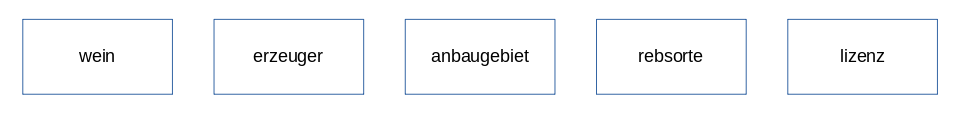
\includegraphics[width=14cm]{images/5.png}
	\caption{Erzeugte \textit{Entity-Typen} mittels Programmcode von Listing \ref{listing3} angewendet auf das Weingut Testmodell}
	\label{ergebnis3}
\end{figure}
\hon{}
\noindent
Die Erstellung der \textit{Attribute} erfolgt nahezu analog zu der Erstellung der \textit{Entity-Typen}. Anstatt der Klasse \verb|RectangleShape| ist die Klasse \verb|EllipseShape| zu verwenden. Falls das \textit{Attribut} ein \textit{Primary-Key} ist, wird der Name des \textit{Attributs} unterstrichen.
\noindent
\\
\\
\noindent
In Abbildung \ref{ergebnis4} sieht man die \textit{Attribute} des \textit{Entity-Typs} Wein: 


\begin{figure}[h]
	\centering
	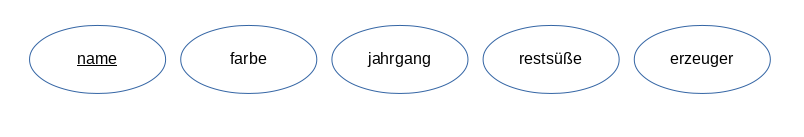
\includegraphics[width=14cm]{images/7.png}
	\caption{Erzeugte Attribute von dem Entity-Typ Wein des Weingut Testmodells}
	\label{ergebnis4}
\end{figure}

\hon{}
\noindent
Im Gegensatz zu Rechtecken oder Ellipsen gibt es keine vordefinierten Formen um \textit{Beziehungstypen} durch eine Raute oder \textit{Super-Sub-Beziehungstypen} durch ein gleichschenkeliges Dreieck darzustellen. An dieser Stelle kommt die Klasse \verb|PolyPolygonShape| zum Einsatz. Mithilfe dieser Klasse und den Funktionen aus Listing \ref{listing5} kann eine Form mit einer beliebigen Anzahl an Seiten erzeugt werden.

\lstset{language=Java}
\lstset{frame=lines}
\lstset{caption={Programmcode in Java, um einen Rechteck mit beliebiger Anzahl an Eckpunkten zu erzeugen}}
\hon{}
\lstset{label={listing5}}
\lstset{basicstyle=\footnotesize}
\begin{lstlisting}
public static XShape drawPolygon(XDrawPage slide, int x, int y, int radius, int nSides, String text) {
    XShape polygon = addShape(slide, "PolyPolygonShape", 0, 0, 0, 0, text);
    Point[] pts = genPolygonPoints(x, y, radius, nSides);
    Point[][] polys = new Point[][] { pts };
    setProperty(polygon, "PolyPolygon", polys);
    return polygon;
}

public static XShape addShape(XDrawPage slide, String shapeType, int x, int y, int width, int height, String text) {
    XShape shape = makeShape(shapeType, x, y, width, height, text);
    if (shape != null){
        slide.add(shape);
    }
    return shape;
}

public static XShape makeShape(String shapeType, int x, int y, int width, int height, String text) {
    XShape shape = null;
    try {
        shape = createInstanceMSF(XShape.class, "com.sun.star.drawing." + shapeType);
        shape.setPosition(new Point(x * 100, y * 100));
        shape.setSize(new Size(width * 100, height * 100));
    } catch (java.lang.Exception e) {
        System.out.println("Unable to create shape: " + shapeType);
    }
    return shape;
}

private static Point[] genPolygonPoints(int x, int y, int radius, int nSides) {
    if (nSides < 3) {
        System.out.println("Too few sides; must be 3 or more");
        nSides = 3;
    } else if (nSides > 30) {
        System.out.println("Too many sides; must be 30 or less");
        nSides = 30;
    }

    Point[] pts = new Point[nSides];
    double angleStep = Math.PI / nSides;
    for (int i = 0; i < nSides; i++) {
        pts[i] = new Point((int) Math.round(x * 100 + radius * 100 * Math.cos(i * 2 * angleStep)),
        (int) Math.round(y * 100 + radius * 100 * Math.sin(i * 2 * angleStep)));
    }
    return pts;
}
\end{lstlisting}
\footfullcite[][]{JavaLibreOfficeProgramming}
\noindent
\\
\hon{}
\\
\noindent
Durch den Aufruf der Funktion \verb|drawPolygon| aus dem Listing \ref{listing5}, die die anderen Funktionen aus dieser Listing aufruft, wird ein Polygon erzeugt. Die Parameter der Funktion haben folgende Bedeutung:
\begin{itemize}
	\item \verb|XDrawPage slide|: beinhaltet die Seite in die das \textit{Polygon} gezeichnet wird.
	\item \verb|int x|: legt den Wert der x-Koordinate fest.
	\item \verb|int y|: legt den Wert der y-Koordinate fest.
	\item \verb|int radius|: legt die Größe der zu zeichnenden Form fest.
	\item \verb|int nSides|: legt die Seitenanzahl der Form fest. Dieser Wert muss zwischen exklusive drei und exklusive dreißig liegen.
	\item \verb|String text|: beinhaltet den Text, der in der Form angezeigt wird.  
\end{itemize}

\noindent
\hon{}
\\
\noindent
Das Ergebnis der Aufrufe \\
\verb|drawPolygon(xDrawPage, 10, 10, 8, 4, "erzeugt");| 
\\ \verb|drawPolygon(xDrawPage, 20, 10, 8, 4, "beinhaltet");| \\ \verb|drawPolygon(xDrawPage, 30, 10, 8, 3, "");| \\
ist in Abbildung \ref{ergebnis5} dargestellt.

\begin{figure}[h]
	\centering
	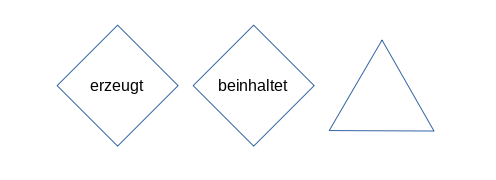
\includegraphics[width=8cm]{images/8.png}
	\caption{Zwei Beziehungstypen und ein Super-Sub-Beziehungstyp}
	\label{ergebnis5}
\end{figure}

\hon{}
\noindent
Um einen \textit{Entity-Typ} mit einem \textit{Beziehungstyp} oder einem \textit{Attribut} zu verbinden, wird die Klasse \verb|XPropertySet| benötigt. Dieser Klasse wird ein Objekt der Klasse \verb|ConnectorShape| mitgegeben. Der Programmcode aus Listing \ref{listing6} zeigt, wie man zwei \textit{Konnektoren} erzeugt und diese von dem \textit{Beziehungstyp} zu zwei verschiedenen \textit{Entity-Typen} verbindet:


\noindent
\lstset{language=Java}
\lstset{frame=lines}
\lstset{caption={Programmcode in Java, um zwei \textit{Konnektoren} zu erzeugen und von einem \textit{Beziehungstyp} zu zwei verschiedenen \textit{Entity-Typen} zu binden}}
\lstset{label={listing6}}
\lstset{basicstyle=\footnotesize}
\begin{lstlisting}

XPropertySet xConnector1PropSet = (XPropertySet) 
UnoRuntime.queryInterface(XPropertySet.class, connector1);
XPropertySet xConnector2PropSet = (XPropertySet) 
UnoRuntime.queryInterface(XPropertySet.class, connector2);

xConnector1PropSet.setPropertyValue("StartShape", diamond);
xConnector1PropSet.setPropertyValue("EndShape", start_shape);
xConnector2PropSet.setPropertyValue("StartShape", diamond);
xConnector2PropSet.setPropertyValue("EndShape", end_shape);

\end{lstlisting}
\noindent
\\
\noindent
Das Ergebnis aus Listing \ref{listing6} wird in Abbildung \ref{ergebnis6} dargestellt.
\begin{figure}[H]
	\centering
	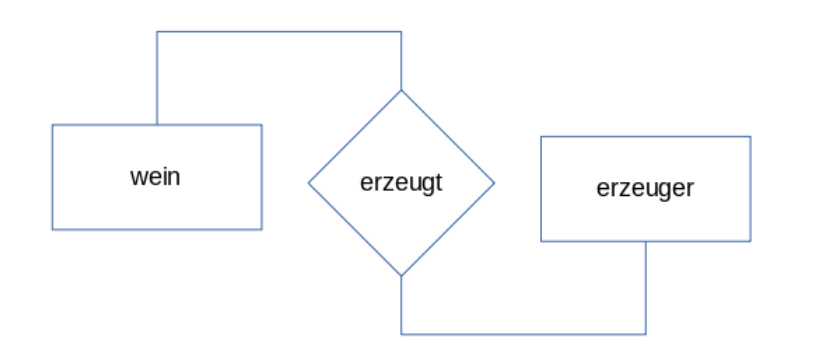
\includegraphics[width=8cm]{images/11.png}
	\caption{Ergebnis aus Listing 4}
	\label{ergebnis6}
\end{figure}
\noindent
Während der Entwicklung über die \textit{API} sind einige Probleme wie zum Beispiel das korrekte Darstellen von \textit{Konnektoren} und \textit{abhängigen Entity-Typen} aufgetreten, weshalb die Weiterentwicklung der Darstellung von \textit{ERDs} über die \textit{API} eingestellt wurde.



\subsubsubsection{Vor- und Nachteile}
\hon{}
\\
Die \textit{LibreOffice API} bietet eine Variante, um ein \textit{LibreOffice}-Dokument zu bearbeiten ohne Modifikationen am Dateiformat vorzunehmen. Dies ist aber nicht der einzige Vorteil:
\begin{itemize}
	\item Die \textit{LibreOffice API} ist zu 100 Prozent kompatibel mit \textit{OpenOffice}. Das bedeutet einerseits, dass das Zielprogramm sowohl ein \textit{LibreOffice} Programm als auch ein \textit{OpenOffice} Programm sein kann, und andererseits, dass es dem Anwendungsprogrammierer frei steht, welche Dokumentation er wählt. 
	\item Darüber hinaus ist sowohl die \textit{LibreOffice API} Dokumentation als auch die \textit{OpenOffice API} Dokumentation sehr umfangreich.
\end{itemize}
\footfullcite[][]{OpenOfficeDevelopersGuide}
\noindent
\\
\noindent
Allerdings bringt diese Methode auch einige Nachteile mit sich:
\\
\begin{itemize}
	\item Die Dokumentation erstreckt sich über 1650 Seiten, was einen einfachen Einstieg in die \textit{API} sehr schwierig macht.
	\item Des Weiteren ist die Dokumentation sehr unübersichtlich und unstrukturiert gestaltet. 
	\item Die Nummerierung der Kapitel und Unterkapitel ist in der Dokumentation nicht angegeben.
	\item Die letzte Version der Dokumentation ist 2009 erschienen und somit veraltet.
	\item Es gibt trotz der langen Entwicklungsgeschichte von \textit{OpenOffice} beziehungsweise \textit{LibreOffice} wenige Anwendungsbeispiele, was ein Erlernen allein durch den Programmcode schwierig gestaltet.
	\item Die Generierung von \textit{ERDs} über die \textit{API} ist ressourcenintensiver und dauert länger als die Generierung über das Dateiformat.
	\item Selbst bei der einfachen Verwendung der \textit{API} müssen oft viele Klassen und Konvertierungen zwischen Klassen erfolgen, um das gewünschte Ergebnis zu erhalten, was das Benutzen der \textit{API} ebenfalls erschwert.   
	\item Viele Objekte, die man in \textit{LibreOffice Draw} händisch erzeugen kann, sind in der \textit{API} nicht vorhanden, wie zum Beispiel ein Dreieck oder eine Raute. Diese müssen dann aufwendig durch die Klasse \verb|PolyPolygonShape| erstellt werden, was einen höheren Programmieraufwand mit sich bringt.
	\item Um die \textit{API} verwenden zu können, ist das \textit{LibreOffice Software Development Kit} notwendig. Dieses muss in jeder Sitzung ausgeführt werden, was Performanceeinbußen mit sich bringt.
\end{itemize}
\footfullcite[][]{OpenOfficeDevelopersGuide}

\noindent
\subsubsection{Generierung über das Dateiformat}
\hon{}



\subsubsubsection{Allgemeines}

\noindent	
\textit{LibreOffice Draw} verwendet das \textit{Open Document Graphics} (ODG) Dateiformat, das 2006 als internationale Norm ISO/IEC 26300 veröffentlicht wurde. 
\textit{ODG} basiert auf einem \textit{XML-Vokabular}, dessen Elemente an den Standard HTML angelehnt sind.
Eine \textit{OpenDocument}-Datei besteht aus einer Sammlung mehrerer \textit{XML-Dateien} und anderer Objekte wie Bilder oder Thumbnails, die zu einer Datei im ZIP-Format zusammengefasst werden.
\\
Bei der Entpackung dieser ZIP-Datei sieht man folgende Dateien und Ordner:
\begin{verbatim}
Datei.odt
|
+-- META-INF
|    |
|    +-- manifest.xml
|
+-- Thumbnails
|    |
|    +-- thumbnail.png
|
+-- Pictures
|    |
|    +-- picture.png
|
+-- mimetype
+-- content.xml
+-- styles.xml
+-- meta.xml
+-- settings.xml
\end{verbatim}
\footfullcite[][]{LibreOfficeWikipedia}

\noindent
Inhalt dieser Dateien:
\hon{}
\begin{itemize}
	\item  \textit{manifest.xml}: In dieser Datei befindet sich eine Übersicht aller Dateien mit deren Pfaden und zulässigen Datentypen.
	\item \textit{thumbnail.png}: Diese Datei zeigt eine Miniaturansicht der ersten Seite des Dokuments.
	\item Im Pictures-Ordner befinden sich alle eingebundenen Bilder des Dokuments. Falls keine Bilder eingebunden sind, existiert dieser Ordner nicht. 
	\item \textit{mimetype}: Diese Datei ist eine Textdatei, deren einziger Inhalt eine Zeile mit dem Typ der \textit{LibreOffice}-Datei ist. Beim Beispiel einer \textit{Draw}-Datei steht folgender Inhalt in der \textit{Mimetype}-Datei: 
	\\
	\verb|application/vnd.oasis.opendocument.graphics|
	\item \textit{settings.xml}: In dieser Datei befinden sich sämtliche \\ Einstellungsmöglichkeiten, die \textit{LibreOffice Draw} anbietet. Darunter fallen zum Beispiel die Maßeinheit, Name und Setup der Drucker, die Skalierung und die Sichtbarkeit der einzelnen Ebenen.
	\item \textit{content.xml}: In dieser Datei befindet sich der eigentliche Inhalt des Dokuments. Durch Betrachtung einer \textit{Draw}-Datei ohne Inhalt ergibt sich die Baumstruktur:
	\begin{verbatim}
	Element: office:document-content
	|
	+-- Attribut: xmlns:--
	+-- Element: office:scripts
	+-- Element: office:font-face-decls
	    |
	    +-- Element: style:font-face
	        |
	        +-- Attribut: style:name
	        +-- Attribut: style:font-family
	        +-- Attribut: style:font-family-generic
	        +-- Attribut: style:font-pitch
	        +-- Element: office:automatic-styles
	            |
	            +-- Element: style:style
	                |
	                +-- Attribut: style:name
	                +-- Attribut: style:family
	                +-- Element: office:body
	                    |
	                    +-- Element: office:drawing
	                        |
	                        +-- Element: draw:page
	                            |
	                            +-- Attribut: draw:name
	                            +-- Attribut: draw:style-name
	                            +-- Attribut: draw:master-page-name
	\end{verbatim}
	
	\noindent
	\hon{}
	\\
	\noindent
	Der komplette Inhalt wird als \textit{XML-Kindelement} von dem \textit{XML-Element} \verb|draw:page| eingefügt.
	In dem \textit{XML-Element} \verb|office:document-content| befinden sich mehrere \textit{XML-Attribute} mit diversen \textit{Namensräumen}, die aus Gründen der \\ Übersichtlichkeit weggelassen wurden.
	
	\item \textit{styles.xml}: Diese Datei beinhaltet die grafischen Informationen der Formatvorlagen für Texte und grafischen Elemente wie zum Beispiel Textfarbe, Textgröße, Füllungsfarbe, Abstand an den Seiten, Rahmenbreite, etc. 
	\item \textit{meta.xml}: In dieser Datei befinden sich Übersichtsinformationen der \textit{LibreOffice}-Datei wie zum Beispiel der Name des Erzeugers, das Datum, an dem das Dokument erstellt wurde, die Sprache des Dokuments und die Bearbeitungsdauer.
	
\end{itemize}
\footfullcite[][]{LibreOfficeWikipedia}
\noindent
\hon{}
\\
\noindent
Wie man in der obigen Auflistung sieht, ist das Dateiformat \textit{ODG} komplex und daher aufwändig zu modifizieren.
\textit{LibreOffice} bietet allerdings auch die Möglichkeit eine \textit{Draw}-Datei in dem Dateiformat \textit{Flat Open Document Graphics} (\textit{FODG}) zu speichern. In diesem Format werden die Dateien aus dem gezippten Ordner zu einer Datei zusammengefasst. Diese Variante der Speicherung ist für die Manipulation des Dateiformats am besten geeignet, da nur eine einzige Datei manipuliert werden muss. 
Für die Manipulation über das Dateiformat wird die Programmiersprache \textit{Python} verwendet. Diese bringt im Zusammenhang mit der gewählten Diplomarbeit mehrere Vorteile mit sich:
\begin{itemize}
	\item In der Regel ist es einfacher und schneller kleinere Programme wie diese Diplomarbeit in \textit{Python} zu entwickeln.
	\item \textit{Python} ist eine plattformunabhängige Sprache, die auf fast allen Betriebssystemen vorhanden ist. 
\end{itemize}

\subsubsubsection{XERML-Daten Aufbereitung in Python}
\hon{}

\noindent
In der Programmiersprache \textit{Python} gibt es mehrere Optionen eine \textit{XML-Datei} zu \textit{parsen} und dessen Daten in ein geeignetes Format für die Weiterverarbeitung zu bringen. Im Zuge der Diplomarbeit ist die Entscheidung auf \textit{LXML} gefallen. \textit{LXML} ist eine \textit{Python}-Bibliothek und bietet einen sicheren und bequemen Zugriff auf die \textit{libxml2} und \textit{libxslt} Bibliothek mithilfe der \textit{ElementTree API}. Die Daten aus der \textit{XML-Datei} werden in einem Array mit dem selben Aufbau wie in Kapitel \ref{XERML-JAVA} gespeichert.


\subsubsubsection{Darstellung der grafischen Elemente}

\noindent
\textbf{Alle Annahmen und Informationen dieses Kapitels entstammen keiner Quelle und wurden durch \textit{Reverse Engineering} in Erfahrung gebracht.}

\hon{}
\noindent
\\
\noindent
Bei jeden Aufruf ein komplettes \textit{LibreOffice} Dokument zu generieren, bedeutet viel Programmieraufwand und beeinträchtigt die Performance. Aus diesem Grund wird das zuvor erstellte leere \textit{LibreOffice} Dokument \textit{empty1.fodg} als Ausgangsdokument verwendet. Um das Dokument auf die Darstellung von \textit{ERDs} zu optimieren, wurden kleinere Modifikationen vorgenommen:
\begin{itemize}
	\item Das Dokument hat einen \textit{Margin} von 1.9 cm.
	\item Sämtliche \verb|gr|, \verb|t| und \verb|p| \textit{XML-Elemente} wurden angepasst. 
	\item Die Informationen über das Format, die Breite und die Höhe wurden entfernt.
\end{itemize} 
\noindent
\hon{}
\\
\noindent
Sämtliche grafische Formen lassen sich mit dem \textit{XML-Element} \verb|custom-shape| erzeugen. Dafür muss man das \textit{XML-Element} als \textit{XML-Kindelement} von dem \textit{XML-Element} \verb|draw:page| einfügen. Das \textit{XML-Element} \verb|custom-shape| benötigt ebenfalls zwei \textit{XML-Kindelemente} um den Text in der grafischen Form anzuzeigen und um die grafischen Eigenschaften der Form festzulegen. Der Aufbau der \textit{XML-Elemente} und deren \textit{XML-Attribute} bei der Erstellung von Rechtecken für \textit{Entity-Typen} und Ellipsen für \textit{Attribute} sieht wie folgt aus:

\begin{verbatim}
Element: draw:page
|
+-- Element: draw:custom-shape
    |
    +-- Attribut: draw:style-name
    +-- Attribut: draw:text-style-name
    +-- Attribut: draw:id
    +-- Attribut: draw:layer
    +-- Attribut: svg:width
    +-- Attribut: svg:height
    +-- Attribut: svg:x
    +-- Attribut: svg:y
    +-- Element: draw:enhanced-geometry
        |
        +-- Attribut: svg:viewBox
        +-- Attribut: draw:mirror-horizontal
        +-- Attribut: draw:mirror-vertical
        +-- Attribut: draw:type
        +-- Attribut: draw:enhanced-path
        +-- Attribut: svg:glue-points
        +-- Attribut: draw:text-areas
        +-- Element: text:p
            |
            +-- Attribut: text:style-name
            +-- Element: text:span
                |
                +-- Attribut: text:style-name

\end{verbatim}
\hon{}
\noindent
Einige der \textit{XML-Attribute} sind für die Erstellung eines \textit{ERDs} unrelevant beziehungsweise werden immer mit den selben Werten befüllt:
\begin{itemize}
	\item Das Attribut \verb|draw:layer| beschreibt die Ebene der Form. Das Ausgangsdokument beinhaltet folgende Ebenen: \textit{layout}, \textit{background}, \textit{backgroundobjects}, \textit{controls} und \textit{measurelines}. Die Ebenen sind absteigend in Richtung Hintergrund geordnet.
	Für die Erstellung eines \textit{ERDs} sind mehrere Ebenen nicht vorgesehen, weshalb dem \textit{XML-Attribut} \verb|draw:layer| immer der Wert \textit{layout} zugeordnet wird.
	\item Mit dem \textit{XML-Attribut} \verb|svg:viewBox| wird eine fixe Pixelbreite und Pixelhöhe festgelegt. Dem Attribut wird immer der Wert \verb|0 0 21600 21600| zugewiesen. 
	\item Die \textit{XML-Attribute} \verb|draw:mirror-horizontal| und \verb|draw:mirror-vertical| bekommen den Wert \verb|false| zugewiesen. 
	\item Das \textit{XML-Attribut} \verb|draw:enhanced-path| bekommt den Wert \verb|U 10800 10800 10800| \verb| 10800 0 360 Z N|.
	\item Das \textit{XML-Attribut} \verb|svg:glue-points| legt die Klebepunkte der Form fest, an denen sich \textit{Konnektoren} anheften können. Diese haben den Wert \verb|10800 0 3163 3163 0| \verb|10800 3163 18437 10800 21600 18437 18437 21600 10800 18437 3163|.
	\item Das \textit{XML-Attribut} \verb|draw:text-areas| bekommt den Wert \verb|3163 3163 18437 18437|.
\end{itemize}
\noindent
\hon{}
\\
\noindent
Der Text wird unter \textit{LXML} mithilfe der Methode \verb|text| bei dem \textit{XML-Element} \verb|text:span| festgelegt.
Das \textit{ERD} kann mit Farbe oder farblos gezeichnet werden. 
Bei einer Darstellung in Farbe werden die Hexadezimalwerte \verb|89D8D6| für \textit{Entity-Typen}, \verb|89BED8| für \textit{Attribute} und \verb|93D889| für \textit{Beziehungstypen} verwendet.
\\
\hon{}

\noindent
Sämtliche Informationen über das Aussehen der Formen werden in den \textit{XML-Elementen} \verb|style:style| gespeichert. Es gibt drei verschiedene Kategorien. Die \verb|gr| \textit{XML-Elemente} speichern die grafischen Informationen. Die \textit{XML-Elemente} \verb|p| und \verb|t| speichern Informationen über die Darstellung von Text. Ein \verb|gr| \textit{XML-Element} könnte wie folgt aussehen:

\begin{verbatim}
<style:style style:name="gr1" style:family="graphic" 
       style:parent-style-name="standard">
    <style:graphic-properties svg:stroke-width="0.03cm" 
           svg:stroke-color="#000000" draw:marker-start-width="0.245cm"
           draw:marker-end-width="0.245cm" draw:fill="solid" 
           draw:fill-color="#ffffff"
           draw:textarea-horizontal-align="justify" 
           draw:textarea-vertical-align="middle"
           draw:auto-grow-height="false" fo:padding-top="0.14cm"
           fo:padding-bottom="0.14cm" fo:padding-left="0.265cm"
           fo:padding-right="0.265cm" style:protect="size"/>
</style:style>
\end{verbatim}
\noindent
\hon{}
\\
\noindent
Um \textit{Entity-Typen} darzustellen, muss das \textit{XML-Attribut} \verb|draw:type| des \textit{XML-Elements} \verb|draw:enhanced-geometry| den Wert \textit{rectangle} beinhalten. Falls die Darstellung in Farbe erwünscht ist, bekommen die \textit{XML-Attribute} die Werte aus der Tabelle \ref{tbl:beispieltabelle1}.
\begin{table}[h]
	\centering
	\begin{tabular}{lll}
		\textbf{Element} & \textbf{Attribut}  & \textbf{Wert} \\
		\\
		draw:custum-shape & draw:style-name           & gr-ent             \\
		draw:custum-shape & draw:text-style-nam      & P-ent             \\
		text:p & text:style-name       & P1             \\
		text:span & text:style-name       & T6             \\
		\\
	\end{tabular}
	
	\caption{Tabelle der \textit{XML-Attributwerte} um \textit{Entity-Typen} farbig darzustellen}
	\label{tbl:beispieltabelle1}
	% Verweis im Text mittels \ref{tbl:beispieltabelle}
	
\end{table}
\noindent
\hon{}
\\

\noindent
Ist ein Darstellen in Farbe nicht erwünscht, bekommen die \textit{XML-Attribute} die Werte aus Tabelle \ref{tbl:beispieltabelle2}

\begin{table}[H]
	\centering
	\begin{tabular}{lll}
		\textbf{Element} & \textbf{Attribut}  & \textbf{Wert} \\
		\\
		draw:custum-shape & draw:style-name           & gr1             \\
		draw:custum-shape & draw:text-style-nam      & P8             \\
		text:p & text:style-name       & P1             \\
		text:span & text:style-name       & T1             \\
		\\
	\end{tabular}
	
	\caption{Tabelle der \textit{XML-Attributwerte} um \textit{Entity-Typen} farblos darzustellen}
	\label{tbl:beispieltabelle2}
	% Verweis im Text mittels \ref{tbl:beispieltabelle}
	
\end{table}

\noindent
Die Breite und Höhe des Rechtecks werden in den \textit{XML-Attributen} \verb|svg:width| und \\ \verb|svg:height| festgelegt. Die Breite ist auf 10 cm und die Höhe ist auf 6 cm festgelegt.
\\
\noindent
Ein \textit{Entity-Typ} könnte in dem Dateiformat \textit{FODG} wie folgt aussehen:
\begin{verbatim}
<draw:custom-shape draw:style-name="gr_ent" draw:text-style-name="P_ent" 
      draw:id="wein" draw:layer="layout" svg:width="10cm" 
      svg:height="6cm" svg:x="159.6cm" 
      svg:y="82.73200000000001cm">
    <text:p text:style-name="P1">
        <text:span text:style-name="T6">wein</text:span>
    </text:p>
    <draw:enhanced-geometry svg:viewBox="0 0 21600 21600" 
          draw:mirror-horizontal="false" 
          draw:mirror-vertical="false" 
          draw:type="rectangle" 
          draw:enhanced-path="M 0 0 L 21600 0 21600 21600 0 21600 0 0 Z N" />
</draw:custom-shape>
\end{verbatim}
\noindent
\hon{}
\\
\noindent
In Abbildung \ref{ergebnis7} ist links das Ergebnis aus dem oben abgebildeten \textit{FODG} zu sehen und rechts ein \textit{Entity-Typ} ohne Farbe.
\begin{figure}[H]
	\centering
	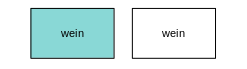
\includegraphics[width=7cm]{images/13.png}
	\caption{Links: Farbiger Entity-Typ in \textit{LibreOffice Draw}. Rechts: Farbloser Entity-Typ in \textit{LibreOffice Draw}}
	\label{ergebnis7}
\end{figure}
\noindent

\hon{}
\noindent
Die Darstellung von \textit{Attributen} funktioniert analog bis auf den Unterschied, dass das \textit{XML-Attribut} \verb|draw:type| den Wert \verb|ellipse| beinhaltet.
Falls ein Darstellen in Farbe erwünscht, bekommen die \textit{XML-Attribute} die Werte aus Tabelle \ref{tbl:beispieltabelle3}.

\begin{table}[H]
	\centering
	\begin{tabular}{lll}
		\textbf{Element} & \textbf{Attribut}  & \textbf{Wert} \\
		\\
		draw:custum-shape & draw:style-name           & gr4             \\
		draw:custum-shape & draw:text-style-nam      & P19             \\
		text:p & text:style-name       & P1             \\
		text:span & text:style-name       & T6            \\
		\\
	\end{tabular}
	
	\caption{Tabelle der \textit{XML-Attributwerte} um \textit{Attribute} farbig darzustellen}
	\label{tbl:beispieltabelle3}
	% Verweis im Text mittels \ref{tbl:beispieltabelle}
	
\end{table}
\hon{}
\noindent
Ist ein Darstellen in Farbe nicht erwünscht, bekommen die \textit{XML-Attribute} die Werte aus Tabelle \ref{tbl:beispieltabelle4}.

\begin{table}[H]
	\centering
	\begin{tabular}{lll}
		\textbf{Element} & \textbf{Attribut}  & \textbf{Wert} \\
		\\
		draw:custum-shape & draw:style-name           & gr1             \\
		draw:custum-shape & draw:text-style-nam      & P8            \\
		text:p & text:style-name       & P1             \\
		text:span & text:style-name       & T1             \\
		\\
	\end{tabular}
	
	\caption{Tabelle der \textit{XML-Attributwerte} um \textit{Attribute} farblos darzustellen}
	\label{tbl:beispieltabelle4}
	% Verweis im Text mittels \ref{tbl:beispieltabelle}
	
\end{table}

\noindent
Ein \textit{Attribut} könnte in dem Dateiformat \textit{FODG} wie folgt aussehen:
\begin{verbatim}
<draw:custom-shape draw:style-name="gr4" draw:text-style-name="P5" 
      draw:id="weinname" draw:layer="layout" svg:width="10cm" 
      svg:height="6cm" svg:x="182.76cm" svg:y="69.76cm">
    <text:p text:style-name="P1">
         <text:span text:style-name="T4">name</text:span>
    </text:p>
    <draw:enhanced-geometry svg:viewBox="0 0 21600 21600" 
          svg:glue-points="10800 0 3163 3163 0 10800 3163 18437 10800 
                           21600 18437 18437 21600 10800 18437 3163"
          draw:type="ellipse" draw:text-areas="3163 3163 18437 18437" 
          draw:enhanced-path="U 10800 10800 10800 10800 0 360 Z N" />
</draw:custom-shape>
\end{verbatim}

\hon{}
\noindent
Falls ein \textit{Attribut} ein \textit{Primary-Key} ist, wird der Name des \textit{Attributs} unterstrichen. Folgende Verwendung von \textit{XML-Attributen} ist dazu notwendig. 
Die \textit{XML-Attribute} bekommen die Werte aus Tabelle \ref{tbl:beispieltabelle5}, falls ein Darstellen in Farbe erwünscht ist.


\begin{table}[H]
	\centering
	\begin{tabular}{lll}
		\textbf{Element} & \textbf{Attribut}  & \textbf{Wert} \\
		\\
		draw:custum-shape & draw:style-name           & gr4             \\
		draw:custum-shape & draw:text-style-nam      & P5             \\
		text:p & text:style-name       & P1             \\
		text:span & text:style-name       & T4            \\
		\\
	\end{tabular}
	
	\caption{Tabelle der \textit{XML-Attributwerte} um \textit{Primary-Key-Attribute} in Farbe darzustellen}
	\label{tbl:beispieltabelle5}
	% Verweis im Text mittels \ref{tbl:beispieltabelle}
	
\end{table}
\noindent
\hon{}
\\
\noindent
Falls die Darstellung in Farbe nicht erwünscht ist, bekommen die \textit{XML-Attribute} die Werte aus Tabelle \ref{tbl:beispieltabelle6}.

\begin{table}[H]
	\centering
	\begin{tabular}{lll}
		\textbf{Element} & \textbf{Attribut}  & \textbf{Wert} \\
		\\
		draw:custum-shape & draw:style-name           & gr1             \\
		draw:custum-shape & draw:text-style-nam      & P7            \\
		text:p & text:style-name       & P1             \\
		text:span & text:style-name       & T4             \\
		\\
	\end{tabular}
	
	\caption{Tabelle der \textit{XML-Attributwerte} um \textit{Primary-Key-Attribute} farblos darzustellen}
	\label{tbl:beispieltabelle6}
	% Verweis im Text mittels \ref{tbl:beispieltabelle}
	
\end{table}
\hon{}
\noindent
In Abbildung \ref{ergebnis8} ist links außen ein farbiges \textit{Attribut} zu sehen, links mittig ein farbiges \textit{Primary-Key-Attribut}, rechts mittig ein \textit{Attribut} ohne Farbe und rechts außen ein farbloses \textit{Primary-Key-Attribut}:
\begin{figure}[H]
	\centering
	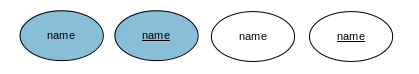
\includegraphics[width=12cm]{images/15.png}
	\caption{Links außen: Farbiges \textit{Attribut}. Links innen: Farbiges \textit{Primary-Key-Attribut}. Rechts innen: Farbloses \textit{Attribut}. Rechts außen: Farbloses \textit{Primary-Key-Attribut}}
	\label{ergebnis8}
\end{figure}
\hon{}
\noindent
Für die Darstellung von Rauten, um \textit{Beziehungstypen} darzustellen, benötigt das \textit{XML-Attribut} \verb|draw:type| den Wert \verb|diamond|. 
Falls ein Darstellen in Farbe erwünscht, bekommen die \textit{XML-Attribute} die Werte aus Tabelle \ref{tbl:beispieltabelle7}.


\begin{table}[H]
	\centering
	\begin{tabular}{lll}
		\textbf{Element} & \textbf{Attribut}  & \textbf{Wert} \\
		\\
		draw:custum-shape & draw:style-name           & gr-rel             \\
		draw:custum-shape & draw:text-style-nam      & P-rel             \\
		text:p & text:style-name       & P1             \\
		text:span & text:style-name       & T6            \\
		\\
	\end{tabular}
	
	\caption{Tabelle der \textit{XML-Attributwerte} um \textit{Beziehungstypen} farblos darzustellen}
	\label{tbl:beispieltabelle7}
	% Verweis im Text mittels \ref{tbl:beispieltabelle}
	
\end{table}
\hon{}
\noindent
Ist die Darstellung in Farbe nicht erwünscht ist, bekommen die \textit{XML-Attribute} die Werte aus Tabelle \ref{tbl:beispieltabelle8}.

\begin{table}[H]
	\centering
	\begin{tabular}{lll}
		\textbf{Element} & \textbf{Attribut}  & \textbf{Wert} \\
		\\
		draw:custum-shape & draw:style-name           & gr1             \\
		draw:custum-shape & draw:text-style-nam      & P8            \\
		text:p & text:style-name       & P1             \\
		text:span & text:style-name       & T1             \\
		\\
	\end{tabular}
	
	\caption{Tabelle der \textit{XML-Attributwerte} um \textit{Beziehungstypen} farblos darzustellen}
	\label{tbl:beispieltabelle8}
	% Verweis im Text mittels \ref{tbl:beispieltabelle}
	
\end{table}
\noindent
\textit{Konnektoren} lassen sich mit dem \textit{XML-Element} \verb|draw:connector| erzeugen.
Um die \textit{Konnektoren} mit einer Start- und Endform verbinden zu können und Text auf dem \textit{Konnektor} darzustellen, wird folgender Aufbau des Elements benötigt:
\begin{verbatim}
Element: draw:page
|
+-- Element: draw:connector
    |
    +-- Attribut: draw:style-name
    +-- Attribut: draw:text-style-name
    +-- Attribut: draw:id
    +-- Attribut: draw:layer
    +-- Attribut: draw:type
    +-- Attribut: start-shape
    +-- Attribut: end-shape
    +-- Attribut: svg:d
    +-- Attribut: svg:viewBox
    +-- Element: text:p
        |
        +-- Attribut: text:style-name
        +-- Element: text:span
            |
            +-- Attribut: text:style-name

\end{verbatim}
\hon{}
\noindent
Die \textit{XML-Attribute} \verb|draw:start-shape| und \verb|draw:end-shape| legen dabei die Start- und Endform fest, wobei sie als Wert die ID der zu verbindenden Form bekommen. Der Text, der auf dem \textit{Konnektor} steht, wird wie bei einem \textit{Entity-Typen} festgelegt. 
\noindent
Ein \textit{Konnektor}, der von einem \textit{Entity-Typ} zu einem \textit{Beziehungstyp} führt, könnte in dem Dateiformat \textit{FODG} wie folgt aussehen:

\begin{verbatim}
<draw:connector draw:style-name="gr2" draw:text-style-name="P3"
      draw:layer="layout" draw:type="line" 
      draw:start-shape="beinhaltet" 
      draw:end-shape="wein" 
      svg:d="M21575 3050l2125 750" 
      svg:viewBox="0 0 2126 751">
    <text:p text:style-name="P1">
        <text:span text:style-name="T1">(1, n)</text:span>
    </text:p>
</draw:connector>
\end{verbatim}
\hon{}
\noindent
Bei \textit{Konnektoren} zwischen einem \textit{Entity-Typ} oder \textit{Beziehungstyp} und einem \textit{Attribut} wird kein Text benötigt und daher entfallen die \textit{XML-Elemente} \verb|text:p| und \verb|text:span|.
\\
\noindent
In Abbildung \ref{ergebnis9} wird die Beziehung zwischen den \textit{Entity-Typen} Anbaugebiet und Erzeuger aus dem Weingut Testmodell.

\begin{figure}[H]
	\centering
	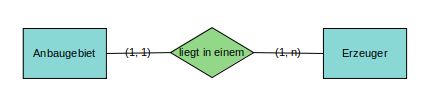
\includegraphics[width=14cm]{images/16.png}
	\caption{Beziehung zwischen den \textit{Entity-Typen} Anbaugebiet und Erzeuger aus dem Weingut Testmodell}
	\label{ergebnis9}
\end{figure}
\hon{}
\noindent
Die komplexeste Form bei der Erstellung von \textit{ERDs} ist ein \textit{Super-Sub-Beziehungstyp}, der als gleichschenkliges Dreieck dargestellt wird. Der Aufbau der \textit{XML-Elemente} sieht für diese Form wie folgt aus:
\begin{verbatim}
Element: draw:page
|
+-- Element: draw:custom-shape
    |
    +-- Attribut: draw:style-name
    +-- Attribut: draw:text-style-name
    +-- Attribut: draw:id
    +-- Attribut: draw:layer
    +-- Attribut: svg:width
    +-- Attribut: svg:height
    +-- Attribut: svg:x
    +-- Attribut: svg:y
    +-- Element: draw:enhanced-geometry
        |
        +-- Attribut: svg:viewBox
        +-- Attribut: draw:mirror-horizontal
        +-- Attribut: draw:mirror-vertical
        +-- Attribut: draw:type
        +-- Attribut: draw:enhanced-path
        +-- Attribut: svg:glue-points
        +-- Element: draw:equation
            |
            +-- Attribut: draw:name
            +-- Attribut: draw:formula

\end{verbatim}	

\noindent
\hon{}
\\
\noindent
Das \textit{XML-Element} \verb|draw:equation| wird dabei achtmal verwendet. (siehe Tabelle \ref{tbl:beispieltabelle9})

\begin{table}[H]
	\centering
	\begin{tabular}{lll}
		\textbf{Element} & \textbf{Wert von draw:name}  & \textbf{Wert von draw:formula} \\
		\\
		Erstes Element \verb|draw:equation| & \verb|f0|           & \verb|$0|              \\
		Zweites Element \verb|draw:equation| & \verb|f1|      & \verb|$0 /2|            \\
		Drittes Element \verb|draw:equation| & \verb|f2|       & \verb|?f1 +10800|             \\
		Viertes Element \verb|draw:equation| & \verb|f3|       & \verb|$0 *2/3|             \\
		Fünftes Element \verb|draw:equation| & \verb|f4|       & \verb|?f3 +7200|             \\
		Sechstes Element \verb|draw:equation| & \verb|f5|       & \verb|21600-?f0|             \\
		Siebtes Element \verb|draw:equation| & \verb|f6|       & \verb|?f5 /2|             \\
		Achtes Element \verb|draw:equation| & \verb|f7|       & \verb|21600-?f6|             \\
		\\
	\end{tabular}
	
	\caption{Werte von den draw:equation Elementen}
	\label{tbl:beispieltabelle9}
	
\end{table}
\noindent
\hon{}
\\
\noindent
Ein \textit{Super-Sub-Beziehungstyp} mit den Werten aus Tabelle \ref{tbl:beispieltabelle9} wird in Abbildung \ref{ergebnis9} gezeigt.
\\
\noindent
Falls der \textit{Beziehungstyp} \textit{disjunkt} ist, bekommt der Maximalwert der Beziehung zu dem \textit{Super-Typen} den Wert \verb|1| und das Dreieck ist \textit{weiß} gefüllt.
Falls der \textit{Beziehungstyp} \textit{nicht disjunkt} ist, bekommt der Maximalwert der Beziehung zu dem \textit{Super-Typen} den Wert der Anzahl der \textit{Sub-Typen} und das Dreieck ist \textit{schwarz} gefüllt.
\\
\\
\noindent
Falls der \textit{Beziehungstyp} \textit{total} ist, bekommt der Minimalwert der Beziehung zu dem \textit{Super-Typen} den Wert \verb|1| und der \textit{Konnektor} zu dem \textit{Super-Typ} ist strichliert, da die eigentliche Darstellung mit zwei parallel verlaufenden Linien unter \textit{Draw} nicht möglich ist.
Falls der \textit{Beziehungstyp} \textit{partiell} ist, bekommt der Minimalwert des \textit{Konnektors} zu dem \textit{Super-Typen} den Wert \verb|0| und der \textit{Konnektor} zu dem \textit{Super-Typ} ist durchgezogen.	
Die \textit{Beziehungskardinalität} zu den \textit{Sub-Typen} ist immer \verb|(1, 1)|.

\begin{figure}[H]
	\centering
	\includegraphics[width=12cm]{images/17.png}
	\caption{\textit{Disjunkter} und \textit{partieller} \textit{Super-Sub-Beziehungstyp} erstellt mit den Werten aus Tabelle \ref{tbl:beispieltabelle9} angewendet auf das Testmodell SIS}
	\label{ergebnis9}
\end{figure}
\noindent
\hon{}
\\
\noindent
\textit{Abhängige Entity-Typen} und \textit{Identifizierende Beziehungstypen} werden mit einer doppelten Umrahmung dargestellt. Dafür werden zwei Rechtecke in das \textit{XML-Element} \verb|draw:g| als \textit{XML-Kindelemente} eingefügt. Die Breite und Höhe des zusätzlichen Rechtecks beträgt 9 cm beziehungsweise 5 cm. Zusätzlich sind die x- und y-Koordinate um 0.5 cm zu verschoben, um den Abstand zwischen den beiden Rechtecken auf jeder Seite gleich zu halten. Ein \textit{abhängiger Entity-Typ} könnte in dem Dateiformat \textit{FODG} wie folgt aussehen:

\begin{verbatim}
<draw:g draw:style-name="gr7" draw:id="kveranst">
    <draw:custom-shape draw:style-name="gr1" draw:text-style-name="P8" 
          draw:layer="layout" svg:width="10cm" svg:height="6cm" 
          svg:x="130.0cm" svg:y="32.62cm">
        <text:p text:style-name="P1">
             <text:span text:style-name="T1"/>
        </text:p>
        <draw:enhanced-geometry svg:viewBox="0 0 21600 21600" 
              draw:mirror-horizontal="false" draw:mirror-vertical="false" 
              draw:type="rectangle" 
              draw:enhanced-path="M 0 0 L 21600 0 21600 21600 0 21600 0 0 Z N"/>
    </draw:custom-shape>
    <draw:custom-shape draw:style-name="gr_ent" 
          draw:text-style-name="P_ent" draw:id="kveranst" 
          draw:layer="layout" svg:width="9cm" svg:height="5cm" 
          svg:x="130.5cm" svg:y="33.12cm">
        <text:p text:style-name="P1">
             <text:span text:style-name="T6">kveranst</text:span>
        </text:p>
        <draw:enhanced-geometry svg:viewBox="0 0 21600 21600" 
              draw:mirror-horizontal="false" draw:mirror-vertical="false" 
              draw:type="rectangle" 
              draw:enhanced-path="M 0 0 L 21600 0 21600 21600 0 21600 0 0 Z N"/>
    </draw:custom-shape>
</draw:g>
\end{verbatim} 
\noindent
\hon{}
\\
\noindent
Das \textit{Primary-Key-Attribut} des \textit{abhängigen Entity-Typen} wird strichliert unterstrichen.
Dafür benötigen die \textit{XML-Attribute} aus Tabelle \ref{tbl:beispieltabelle9} jene Werte, falls das Darstellen in Farbe erwünscht ist.

\begin{table}[H]
	\centering
	\begin{tabular}{lll}
		\textbf{Element} & \textbf{Attribut}  & \textbf{Wert} \\
		\\
		draw:custum-shape des äußeren Rechtecks & draw:style-name           & gr1             \\
		draw:custum-shape des äußeren Rechtecks & draw:text-style-nam      & P8            \\
		text:p des äußeren Rechtecks & text:style-name       & P1             \\
		text:span des äußeren Rechtecks & text:style-name       & T1             \\
		draw:custum-shape des inneren Rechtecks & draw:style-name           & gr-ent             \\
		draw:custum-shape des inneren Rechtecks & draw:text-style-nam      & P-ent            \\
		text:p des inneren Rechtecks & text:style-name       & P1             \\
		text:span des inneren Rechtecks & text:style-name       & T6             \\
		\\
	\end{tabular}
	
	\caption{Tabelle der \textit{XML-Attributwerte} um \textit{Primary-Key-Attribute} von \textit{abhängigen Entity-Typen} in Farbe darzustellen}
	\label{tbl:beispieltabelle9}
	% Verweis im Text mittels \ref{tbl:beispieltabelle}
	
\end{table}
\noindent
\hon{}
\\
\noindent
Ist die Darstellung in Farbe nicht erwünscht ist, bekommen die \textit{XML-Attribute} die Werte aus Tabelle \ref{tbl:beispieltabelle10}. 

\begin{table}[H]
	\centering
	\begin{tabular}{lll}
		\textbf{Element} & \textbf{Attribut}  & \textbf{Wert} \\
		\\
		draw:custum-shape des äußeren Rechtecks & draw:style-name           & gr1             \\
		draw:custum-shape des äußeren Rechtecks & draw:text-style-nam      & P8            \\
		text:p des äußeren Rechtecks & text:style-name       & P1             \\
		text:span des äußeren Rechtecks & text:style-name       & T1             \\
		draw:custum-shape des inneren Rechtecks & draw:style-name           & gr1             \\
		draw:custum-shape des inneren Rechtecks & draw:text-style-nam      & P8            \\
		text:p des inneren Rechtecks & text:style-name       & P1             \\
		text:span des inneren Rechtecks & text:style-name       & T1             \\
		\\
	\end{tabular}
	
	\caption{Tabelle der \textit{XML-Attributwerte} um \textit{Primary-Key-Attribute} von \textit{abhängigen Entity-Typen} farblos darzustellen}
	\label{tbl:beispieltabelle10}
	% Verweis im Text mittels \ref{tbl:beispieltabelle}
	
\end{table}	


\noindent
\hon{}
\\
\noindent
Die Abbildung \ref{ergebnis10} zeigt einen \textit{identifizierenden Beziehungstyp} und einen \textit{abhängigen Entity-Typen} mit dessen \textit{Primary-Key-Attribut}.


\begin{figure}[H]
	\centering
	\includegraphics[width=12cm]{images/18.png}
	\caption{\textit{Identifizierender Beziehungstyp} und ein \textit{abhängigen Entity-Typ} mit dessen \textit{Primary-Key-Attribut}}
	\label{ergebnis10}
\end{figure}	

\subsubsubsection{IDs}
\hon{}

\noindent
Eine zentrale Rolle in der Generierung von \textit{ERDs} über das Dateiformat spielen die IDs der Formen. Ohne diese wäre es nicht möglich \textit{Konnektoren} an \textit{Entity-Typen}, \textit{Attributen} oder \textit{Beziehungstypen} zu verankern. Da eine ID eindeutig sein muss, reicht der Name eines \textit{Attributes} oder eines \textit{Beziehungstyps} meist nicht aus, da dieser meist öfter als einmal vorkommen kann. Aus diesem Grund werden die IDs aus mehreren Faktoren zusammengesetzt:
\begin{itemize}
	\item Die ID eines \textit{Entity-Typs} ist dessen Name. Dieser muss eindeutig sein und reicht daher aus.
	\item Die ID eines Attributs setzt sich aus dem Namen des zugehörigen \textit{Entity-Typs} und dem Namen des Attributs zusammen.
	\item Die ID eines \textit{Beziehungstyps} ist dessen Name. Dieser muss eindeutig sein und reicht daher aus.
	\item Die ID eines \textit{Beziehungsattributs} setzt sich aus dem Namen der zugehörigen Beziehung und dem Namen des Attributs zusammen.
	\item Die ID einer \textit{Super-Sub-Beziehung} setzt sich aus dem Namen der \textit{Super-Sub-Beziehung} und dem Suffix \textit{super-sub} zusammen.
\end{itemize} 


\subsubsubsection{Vor- und Nachteile}
\hon{}
\\
\noindent
Die Erstellung eines \textit{ERDs} in \textit{LibreOffice Draw} über das Dateiformat bringt folgende Vorteile mit sich:
\begin{itemize}
	\item Durch \textit{Reverse Engineering} lässt sich sehr schnell die Bedeutung der einzelnen \textit{XML-Elemente} und \textit{XML-Attribute} herausfinden, was ein schnelles Einlesen in das Dateiformat ermöglicht.
	\item Die Erzeugung einer \textit{XML-Datei} in \textit{Python} ist sehr performant im Vergleich zu der Verwendung der \textit{LibreOffice API} (siehe Abschnitt \ref{performance}).
\end{itemize}
\noindent
Allerdings bringt diese Variante auch einige Nachteile mit sich:
\begin{itemize}
	\item Die Modifikation des Dateiformats ist sehr heikel. Ein falsches Einrücken oder das Erzeugen eines nicht vorhandenen \textit{XML-Attributs} reicht, um die \textit{FODG}-Datei nicht mehr öffnen zu können.
	\begin{figure}[H]
		\centering
		\includegraphics[width=7cm]{images/21.png}
		\caption{Fehlermeldung in \textit{LibreOffice Draw}, falls das Dateiformat ungültig ist.}
		\label{ergebnis10}
	\end{figure}
	
	\item Es gibt keine Dokumentation, in der das Dateiformat beschrieben steht.
\end{itemize}


\subsubsection{Performancevergleich}
\label{performance}
\hon{}

Bei der Generierung der Testmodelle ist ein klarer Performanceunterschied erkennbar. Um diesen Unterschied zu veranschaulichen, wurde jedes Testmodell in beiden Generierungsvarianten generiert und dabei die benötigte Zeit gemessen. Um mögliche Ausreißer zu eleminieren, wurde jedes Testmodell fünfmal pro Generierungsvariante generiert und danach wurde der Durchschnitt gebildet. Die Testmodelle wurden in Farbe und mit Attributen generiert. Die Ergebnisse des Vergleichs sind in Tabelle \ref{tbl:performance} veranschaulicht.

\begin{table}[H]
	\centering
	\begin{tabular}{lll}
		\textbf{Testmodell} & \textbf{Benötigte Zeit API}  & \textbf{Benötigte Zeit Dateiformat} \\
		\\
		AAA & 29,61 Sekunden           & 0,52 Sekunden             \\
		Fußball & 25,02 Sekunden      & 0,31 Sekunden            \\
		Kinokette & 28,50 Sekunden       & 0,46 Sekunden           \\
		Mondial & 93,79 Sekunden       & 12,03 Sekunden             \\
		Rettungsstelles & 32,95 Sekunden           & 0,72 Sekunden             \\
		SF & 40,32 Sekunden      & 0,16 Sekunden            \\
		SIS & 29,83 Sekunden       & 0,45 Sekunden             \\
		Tankstelle & 25,99 Sekunden       & 0,36 Sekunden             \\
		Weingut & 18,86 Sekunden       & 0,15 Sekunden             \\
		\\
	\end{tabular}
	
	\caption{Benötigte Zeit jedes Testmodells in den beiden Generierungsvarianten.}
	\label{tbl:performance}
\end{table}
\noindent
\hon{}
\\

\noindent
Folgende Soft- beziehungsweise Hardware wurde für die Generierung der Testmodelle verwendet:

\begin{itemize}
	\item OS: Linux Mint virtualisiert mittels Oracle VM VirtualBox
	\item CPU: Intel Core i5-6600k @ 3,9GHz
	\item GPU: GeForce GTX 980 Ti
	\item RAM: 16GB @ 2666MHz
\end{itemize}


\subsection{Layout}
\hon{}
\noindent
Um ein aufwendiges Nachbearbeiten des \textit{ERDs} zu verhindern, wird das \textit{ERD} mit einem Layout erzeugt. Als Layoutalgorithmus wurde \textit{Graphviz} verwendet. (siehe Kapitel \ref{layout})








	

\section{Git}
\fib{}

\noindent
Bei einem Projekt mit diesem Umfang ist es von Vorteil jegliche Art von Versionsverwaltung zu verwenden. Außer Git hätten sich noch andere Versionsverwaltungssysteme angeboten wie z.B.:
\footcite{noauthor_git_2019}
\begin{itemize}
	\item Mercurial
	\item Darcs
	\item Fossil
	\item Bazaarn	
\end{itemize}

\noindent
Jedoch wurde für dieses Projekt gezielt Git verwendet. Git ist unter den Versionverwaltungssystemen das gängigste und deswegen existiert dafür auch der meiste Support. Außerdem verwendet Trac, die Projektorganisations-Web-App die in diesem Projekt verwendet wurde, Git deswegen waren die anderen Möglichkeiten nicht mit Git gleichwertig. 
\\

\noindent
Durch gezieltes anlegen von Branches wurde es ermöglicht jedem Entwickler eine vollkommen von den Anderen unabhängige Entwicklungsumgebung zu bieten. 
Diese sogenannten Feature-Branches ermöglichten es, unabhängig vom derzeitigen Entwicklungsstands des Projekts, es zu jederzeit eine funktionierende Version der Software am Master-Branch vorlag.
\\

\noindent
Die Daten lagen zu jeder Zeit auf dem Server, den der Auftraggeber bereitgestellt hat, vor und ermöglichte dadurch eine einfachen Zugriff. Mit einem unabhängigen Server ist es den Entwicklern leicht gefallen von zu Hause und in der Schule immer am neusten Stand zu sein.
\\

\newpage
\section{Trac}
\fib{}

\noindent
Trac ist eine Software die bei der Entwicklung und Organisation des Projekts eine große Hilfe ist. Dadurch wird ein Interface für Versionsverwaltung geboten, sowie ein für Scrum ideales Ticketsystem. Außerdem bietet es einen Aktivitätsüberblick und einen Überblick über den aktuellen Stand des Projekts in Form von einer Roadmap.
\footcite{noauthor_trac_nodate}

\noindent
Durch das Ticketsystem kann man mit Leichtigkeit die verschiedenen Aufgaben verteilen und feststellen ob sie fertiggestellt wurden.
\\
\begin{figure}[h]
	\begin{center}
		\includegraphics[width=16cm]{images/Trac_Tickets.png}
		\caption{Ticket im Trac}
		\label{Trac Ticket}
	\end{center}
\end{figure}

\noindent
Trac unterstützt WikiFormatting, mithilfe diesem Merkmals kann man eine angenehme und leicht leserliche Struktur erschaffen.

\noindent
Davon war das erstellen von Links auf interne Ressourcen sowie auf externe Ressourcen eine der meist verwendeten Funktionen.
\begin{figure}[h]
	\begin{center}
		\includegraphics[width=16cm]{images/Trac_Links.png}
		\caption{Dokumentation für Links im Trac}
		\label{Trac Links}
	\end{center}
\end{figure}




\newpage

\section{Sphinx}
\pra
\noindent
Das Werkzeug \textit{Sphinx} wird verwendet, um eine Dokumentation zu erstellen. Diese wird dabei in gutem Layout automatisch generiert. Der Benutzer kann nach der Erstellung noch händische Änderungen vornehmen, falls er noch weitere Informationen zu der Dokumentation hinzufügen möchte oder der generierte Inhalt nicht korrekt ist. 
\\

\noindent
Sphinx wurde ursprünglich für die \textit{Python Dokumentation} erstellt und bietet einige Möglichkeiten, eine Dokumentation für Softwareprojekte in verschiedenen Sprachen zu generieren \footfullcite{sphinx}. 
\\

\noindent
Die erstellte Dokumentation kann als Dokumenttypen folgende Formate annehmen\footnotemark[31]: 
\begin{itemize}
	\item{HTML}
	\item{LaTeX}
	\item{ePub}
	\item{Texinfo}
	\item{Manual pages}
	\item{plain text}
\end{itemize}

\subsection{Generierung der Dokumentation}\pra
\noindent
Um die Dokumentation automatisch generieren zu können, muss das Skript \verb|sphinx-quickstart| ausgeführt werden. Dieses Skript erstellt ein \textit{Source}-Verzeichnis und die Datei \textit{conf.py}, in der die sinnvollste Konfiguration angegeben wird. Diese Konfigurationsdatei wird anhand der Angaben erstellt, die in dem Befehl \verb|sphinx-quickstart| eingegeben wurden. Zum Beispiel stellt der Befehl die Frage, ob \textit{autodoc} verwendet werden soll. Diese Frage ist mit \textit{JA} zu beantworten, weil sonst die Dokumentation nicht automatisch generiert werden kann \footnotemark[31].
\\

\noindent
Sobald dieser Befehl vollständig ausgeführt wurde, wird eine weitere Datei \textit{index.rst} erstellt. Der Zweck dieses Dokuments ist im Grunde, dass ein Deckblatt und ein Inhaltsverzeichnis generiert werden \footnotemark[31].
\\

\noindent
Um Inhalte hinzuzufügen, können einige Features von \textit{reStructuredText} verwendet werden. Zum Beispiel kann als Richtlinie \textit{toctree} verwendet werden. \textit{toctree} kann verglichen werden mit \textit{Markup}, jedoch ist \textit{toctree} um einiges vielseitiger \footnotemark[31]. 
\\

\noindent
Um Dokumente in die Dokumentation beziehungsweise Einträge in das Inhaltsverzeichnis hinzuzufügen müssen die jeweiligen Dateien in dem \textit{toctree} angegeben werden. Ein \textit{toctree} mit zwei Elementen sieht zum Beispiel wie folgt aus\footnotemark[31]:
\pra
\begin{verbatim}
..toctree...
  :maxdepth: 2
  
  usage/installation
  usage/quickstart

\end{verbatim}
\noindent
Um die ganze Dokumentation zu erstellen, muss der Befehl
\begin{verbatim}
     sphinx-build -b html sourcedir builddir
\end{verbatim} 
ausgeführt werden. Der Parameter \verb|-b| gibt an, in welchem Format die Dokumentation erstellt werden soll. In dem obigen Beispiel hat die Dokumentation den Dateitypen \textit{HTML}. Das Argument \verb|sourcedir| setzt den Ordner, wo die zu generierende Dokumentation enthalten ist und \verb|builddir| gibt an, wo die generierte Dokumentation gespeichert werden soll.\footfullcite{sphinx}
\\

\noindent
Die Dokumentation kann jedoch auch mit Hilfe einer anderen Möglichkeit generiert werden. Das Skript \verb|sphinx-quickstart| erzeugt zusätzlich noch eine \textit{Makefile} und ein Dokument \textit{make.bat}. Um das \textit{Makefile} auszuführen wird folgende Anweisung benötigt\footnotemark[32]:
\\

\begin{verbatim}
     make html
\end{verbatim}
\noindent
Der Parameter \textit{html} gibt an, dass der Typ der Dokumentation eine \textit{HTML}-Datei ist. Falls jedoch nur der Befehl \verb|make| ohne weitere Parameter angegeben wird, wird eine Hilfe mit allen möglichen Zieldokumenten in dem gewünschten Ordner ausgegeben \footnotemark[32].
\\
\subsection{Aufbau der Dokumentation}
\pra
\noindent
Das Grundgerüst der Dokumentation für das Projekt wurde mit Hilfe von Sphinx automatisch generiert. Weitere Informationen wie unter anderem Beispielaufrufe müssen per Hand geschrieben werden.
\\

\noindent
Zu Beginn der Dokumentation befindet sich ein Deckblatt mit allen Autoren. Anschließend bietet ein Inhaltsverzeichnis eine kleine Übersicht an. Nach diesem beginnt Kapitel 1 mit einer kurzen Anleitung, wie das Projekt installiert werden kann. 
\\

\noindent
In Kapitel 2 der Dokumentation werden alle Befehle aufgelistet, wobei jeder Befehl über eine eigene Sektion verfügt. In jeder dieser Sektionen werden ebenfalls alle gültigen Parameter sowie mindestens ein Beispielaufruf angegeben. 
\\

\noindent
Das Projekt verfügt über zwei unterschiedliche Hauptfunktionalitäten. Diese teilen sich in das Generieren eines \textit{Entity Relationsip Diagrammes} und in das Erzeugen von \textit{Data Manipulation Language}-Kommandos auf. In der Dokumentation werden zuerst die Befehle aufgezählt, die für das Erstellen eines \textit{ERDs} verwendet werden können. Zu diesen Befehlen gehören:
\\

\noindent
\begin{itemize}\pra
	\item{\verb|erdgenerate|} 
	
	\item \verb|open|
		
	\item \verb|exit| 
	
	\item \verb|shell| 
	
	\item \verb|bye|
	
	\item \verb|list|
	
	\item \verb|erdfocus|
	
	\item \verb|blockdiagram|
	\\
\end{itemize}

\noindent
Nach den bereits aufgelisteten Befehlen für die Erstellung eines \textit{ERDs} werden alle Befehle zur Generierung von \textit{DML}-Kommandos aufgezählt:
\\

\noindent
\begin{itemize} \pra
	\item \verb|dmlgenerate|
	
	\item \verb|dmlform|
	
	\item \verb|config|

	\item \verb|basex| 
	
	\item \verb|oracle| 
	
	\item \verb|postgresql|
	
	\item \verb|sqlite| 
	
	\item \verb|sqlserver|
	
	\item \verb|mysql|
	\\
\end{itemize}

\noindent
Die Sektion, die den Befehl \verb|erdgenerate| beschreibt, sieht wie folgt aus:

\begin{verbatim}
2.3.1 erdgenerate
Generate an ERD from XERML Modell

ermtk erdgenerate [-h] [-i INPUTFILE] [-n NOTATION] [-t TYP] [-a]
                  [-c] [-g] [-p] [-d] [-v] [-l LOC] [-s] [--auto]
Named Arguments
    -i, --inputfile      Inputfile
    -o, --output         Outputfile
    -n, --notation       Takes a value to define the notation
    -t, --typ            Attributes with types are displayed in the ERD
    -a, --attr           The ERD displays Attributes
    -c, --color          The ERD is colored
    -g, --graphml        The Output-Type is a GraphML File
    -p, --pic            The Output-Type is a PIC File
    -d, --draw           The Output-Type is a Libre Office Draw File
    -v, --viz            The Output-Type is a Graphviz File
    -l, --loc            Define the output language
    -s, --show           Shows generated Diagram in Programm
    --auto               ERD generated with default options
EXAMPLES

    ermkt erdgenerate -i sis.xerml.xml -o sis.graphml -g
    ermkt erdgenerate -o sis.xerml.xml -o sis.graphml -n crowfoot -g
\end{verbatim}\pra

\chapter{Testmodelle}
\label{cha:Testmodelle}
\fib{}
\section{Überblick}

\noindent
Bei dem Projekt gab es 9 Testmodelle die wären:
\begin{itemize}
    \item Fußball
    \item Kinokette
    \item Mondial
    \item Rettungsstelle
    \item Schulungsfirma
    \item Schulinformationssystem
    \item Tankstellenkette
    \item Weingut
\end{itemize}
\noindent

\noindent
Jedes dieser Testmodelle stellt eine Datenbank da. Alle 9 mussten in Form eine XERML-Datei erstellt werden um sie dann mit den vier verschiedenen Programmen zu verarbeiten. Darin sollten alle Variationen vorhanden sein z.B. Vererbungen, Abhängige-Typen usw..

\noindent
Diese XERML-Dateien können mit einem Tool eines anderen Projekts automatisch generiert werden.
Sie bestehn in der Regel aus drei verschiedenen Dateien.
\begin{itemize}
    \item Grunddatei mit der Endung "xerml.xml", in dieser Datei steht der grobe Aufbau des Modells.
    \item Sprachdatei wo verschiedene Übersetzungen enthalten sind mit der Endung "xerml.lo.xml".
    \item Typdatei die die einzelnen Attribute einer Entity beschreibt mit der Endung "xerml.ty.xml".
\end{itemize}


\newpage
\section{Schulinformationssystem}
\prc

Das Testmodell ,,Schulinformationssystem'' soll das Datenmodell für eine HTL abbilden. Dabei waren folgenden Punkte aus dem Skriptum \cite{skriptum} zu berücksichtigen:

\begin{enumerate}
	\item Die abteilungsweise Gliederung einer HTL ist wiederzugegeben.
	\item Jeder Lehrer ist einer Abteilung als Stammabteilung zugeordnet, kann aber auch in Klassen anderer Abteilungen unterrichten. Jede Abteilung wird von einem Lehrer als Abteilungsvorstand geleitet.
	\item Für jede Ausbildungsform der Abteilungen ist im Lehrplan festgehalten, welche Gegenstände in welchen
	Jahrgängen, in welchem Ausmaß (Theorie- und Übungsstunden) unterrichtet werden müssen.
	\item Die Klassen eines Schuljahres werden von den Lehrern in den einzelnen Gegenständen in einem bestimmten
	Stundenausmaß (Theorie- und Übungsstunden) unterrichtet.
	\item Jeder Schüler wird mit einer Semester- und einer Jahresnote pro Klasse und Gegenstand beurteilt. In dem
	System sollen diese Informationen für mehrere Schuljahre festgehalten werden können.
	\item Die Klassenvorstände der verschiedenen Klassen sollen feststellbar sein, ebenso von welchem Schüler welche Funktionen (Klassensprecher, Kassier, etc.) ausgeübt werden oder wurden.
	\item Die Entlohnung der Lehrer erfolgt nicht nach gehaltenen Stunden, sondern nach gehaltenen Werteinheiten:
	jeder Gegenstand ist einer bestimmten Lehrverpflichtungsgruppe (LVG) (I bis VI) zugeordnet. Für jede LVG
	ist ein Faktor (1,167 bis 0,75) festgelegt, der zur Umrechnung von Stunden in Werteinheiten herangezogen
	wird.
	\item Für jeden Schüler ist ein Erziehungsberechtigter verantwortlich (sofern der Schüler nicht eigenberechtigt
	ist). Wenn Geschwister die Schule besuchen, soll dies ebenfalls ermittelt werden können.
	\\
\end{enumerate} 

\noindent
Diese Punkte ließen auf die folgenden Entitytypen schließen:

\begin{multicols}{2}
	\begin{itemize}
		\item Person
		\item Lehrer
		\item Schüler
		\item Abteilung
		\item Gegenstand
		\item Klasse
		\item Lehrverpflichtungsgruppe
		\item Lehrplan
	\end{itemize}
\end{multicols}

\noindent
Um das Datenmodell vollständig abzubilden sind auch Beziehungen zwischen den Entiytypen nötig. Um zum Beispiel den 2. Punkt der Aufgabe zu realisieren, wurden folgende Beziehungstypen definiert:

\begin{lstlisting}[language=XML, caption={XERML-Definition von Punkt 2 der Angabe}]
<!-- Punkt 2-->
<rel to="gehört zu">
   <part ref="Lehrer" min="1" max="1"/>
   <part ref="Abteilung" min="1" max="n"/>
</rel>

<rel to="wird geleitet" from="leitet">
   <part ref="Abteilung" min="1" max="1"/>
   <part ref="Lehrer" min="0" max="1"/>
</rel>
\end{lstlisting}

\noindent
Die komplette Umsetzung des Datenmodells befindet sich im Anhang.

\section{Rettungsstelle}
\fib{}

\noindent
Die Rettungsstelle soll den Aufbau einer echten Rettungsstelle darstellen und dabei veranschaulichen welche Vorgänge bzw. Ressourcen miteinander in Beziehung stehen.
Das Datenmodell der Rettungsstelle besteht aus sieben Entity-Typen:

\begin{itemize}
    \item Einsatz oder auch mission
    \item Fahrt oder auch trip
    \item Person oder auch person
    \item Angestellter oder auch employee
    \item Patient oder auch patient
    \item Auto oder auch car
    \item Gragage oder auch garage
\end{itemize}

\noindent
Zwischen diesen Entity-Typen existieren sechs Relationen und jede dieser Relationen kann man mit je zwei Sätzen beschreiben.
\begin{itemize}
    \item Ein Einsatz besteht aus keiner oder mehreren Fahrten.\newline
          Eine Fahrt ist Bestandteil genau eines Einsatzes.
    \item Ein Mitarbeiter nimmt an keiner oder mehreren Fahrten teil. \newline
          Bei einer Fahrt ist mindestens ein Mitarbeiter oder mehrere Mitarbeiter beteiligt. 
    \item Ein Patient wird bei genau einem Einsatz gerettet. \newline
          Bei einer Fahrt wird mindestens ein Patient oder mehrere Patienten gerettet. 
    \item Ein Auto wird bei mindestens einer Fahrt oder mehreren Fahrten verwendet. \newline
          Bei einer Fahrt wird genau ein Auto verwendet.
    \item Ein Auto hat mindestens eine Garage oder mehrere Garagen. \newline
          In einer Garage steht genau ein Auto.
    \item Patient ist eine Person mit einer SVN, KVA, Einsatzbeschreibung, Kennzeichen, Einsatznummer. \newline
          Angestellter ist eine Person mit einer Mittarbeiternummer, Rang, Schulung, Kennzeichen, Einsatznummer.
\end{itemize}

\noindent

\newpage
 
\section{Fußball}
\pra

\noindent
Für die Erstellung des Datenmodells \textit{Fußball} wurden folgende Annahmen getroffen:

\begin{itemize}
	\item Jede Mannschaft hat einen eindeutigen Namen, ein bestimmtes Gründungsjahr und ist an einer bestimmten Adresse beheimatet.
	\item Zu jeder Mannschaft gehören Fußballspieler.
	\item Ein Spieler kann durch die SVNr identifiziert werden. Weiters hat ein Spieler einen Namen, eine Wohnadresse, ein Geburtsdatum und eine Position, an der er spielt.
	\item Die Mannschaften beteiligen sich an Spielen. 
	\item Die Spiele können durch die Adresse des Stadions, dem Tag und der Uhrzeit eindeutig festgelegt werden.
	\item Pro Spiel werden die beteiligten Mannschaften sowie der Schiedsrichter und das Ergebnis gespeichert.
	\item Falls das Spiel zu einem Turnier gehört, soll diese Information ebenfalls gespeichert werden.
	\item Die Anzahl der Tore, die in einem Spiel geschossen wurden, sollen gespeichert werden.
	\item Ein Schiedsrichter verfügt über die gleichen Daten wie ein Spieler ausser dass er keine Spielposition hat. Dafür wird bei dem Schiedsrichter das Datum der Schiedsrichterprüfung und die Berechtigungsklasse gespeichert.
	\item Jedes Turnier hat eine eindeutige Nummer, einen Namen, ein Beginn- und Enddatum und die beteiligten Mannschaften gespeichert.
\end{itemize}

\noindent
Anhand all dieser Annahmen entsteht folgendes Datenmodell:\pra
\begin{verbatim}
<erm version="0.2">

<!-- Front Matter -->

<title name="Fussball"/>
<title name="soccer" lang="en"/>

<!-- Entity-Types -->

<ent name="mannschaft">
    <attr name="name" prime="true"/>
    <attr name="gründungsjahr"/>
    <attr name="adresse"/>
</ent>

<ent name="person">
    <attr name="svnr" prime="true"/>
    <attr name="name"/>
    <attr name="wohnadresse"/>
    <attr name="geburtsdatum"/>
</ent>

<ent name="spieler">
    <attr name="spielposition"/>
</ent>

<ent name="spiel">
   <attr name="spielort" prime="true"/>
   <attr name="datum"    prime="true"/>
   <attr name="mannschaft_heim"/>
   <attr name="mannschaft_ausw"/>
   <attr name="schiedsrichter"/>
   <attr name="ergebnis"/>
</ent>

<ent name="turnier">
   <attr name="nummer" prime="true"/>
   <attr name="name"   prime="true"/>
   <attr name="beginndatum"/>
   <attr name="enddatum"/>
   <attr name="mannschaften"/>
</ent>
 
<ent name="schiedsrichter">
   <attr name="datum_prüfung"/>
   <attr name="berechtigungsklasse"/>
</ent>

<ent name="tore">
   <attr name="anzahl_tore"/>
</ent>

\end{verbatim}

\noindent
Die \textit{Entities} stehen wie folgt in Beziehung miteinander:
\pra
\\

\begin{verbatim}
<rel to="ist ein">
    <super ref="person" total="false" disjoint="true"/>
        <sub ref="spieler"/>
        <sub ref="schiedsrichter"/>
</rel>

<rel to="spielt bei">
    <part ref="spieler" min="1" max="1"/>
    <part ref="mannschaft" min="1" max="n"/>
</rel>

<rel to="spielt mit bei">
    <part ref="mannschaft" min="1" max="n"/>
    <part ref="spiel" min="1" max="n"/>
</rel>

<rel to="gehört zu">
    <part ref="spiel" min="0" max="1"/>
    <part ref="turnier" min="1" max="n"/>
</rel>

<rel to="pfeift bei">
    <part ref="schiedsrichter" min="1" max="1"/>
    <part ref="spiel" min="1" max="1"/>
</rel>

<rel to="hat geschossen">
    <part ref="tore" min="0" max="n"/>
    <part ref="spieler" min="0" max="n"/>
</rel>

<rel to="wurden geschossen">
    <part ref="tore" min="0" max="n"/>
    <part ref="spiel" min="0" max="n"/>
</rel>
</erm>

\end{verbatim}
\pra

\section{Weingut}
\hon{}
\noindent
Im Umfang der Diplomarbeit ist die Erstellung einer \textit{XERML}-Testmodells von jedem Diplomanden beinhaltet, um die zu entwickelnde Software mit den Modellen testen zu können.
\\
\noindent
Gefordert ist das Modell eines Weinguts, in dem verschiedene Erzeuger diverse Weine anbieten. Jeder Erzeuger liegt in einem Anbaugebiet und hat eine Lizenz, die es dem Erzeuger ermöglicht eine bestimme Menge Wein zu erzeugen. Die Weine bestehen jeweils zu einem bestimmten Anteil aus verschiedenen Rebsorten.


\subsection{Die Hauptdatei}
\hon{}

\noindent
Bei der Modellierung der Hauptdatei \textit{weingut.xerml.xml} kommt es zu mehreren Varianten der \textit{Beziehungen} oder \textit{Attribute}. Um das \textit{XERML} so realistisch und einfach wie möglich zu halten, wurden folgende Annahmen getroffen:
\begin{itemize}
	\item Der Name des Weins ist der \textit{Primary-Key}, da es in der Realität nicht mehrere Weine mit dem selben Namen gibt. 
	\item Der Name und die Adresse des Erzeugers bilden den \textit{Primary-Key}, da es keine Erzeuger mit demselben Namen und derselben Adresse geben kann.
	\item Der Name und die Region des Anbaugebiets ist der \textit{Primary-Key}, da es nicht mehrere Anbaugebiete mit demselben Namen in derselben Region geben kann.
	\item Der Name einer Rebsorte ist eindeutig und daher der alleinige \textit{Primary-Key}. 
	\item Die Lizenznummer einer Lizenz ist eindeutig und daher der alleinige \textit{Primary-Key}.
	
	\item Ein bestimmter Erzeuger kann mehrere Weine erzeugen und ein bestimmter Wein kann von mehreren Erzeugern erzeugt werden. Ein Erzeuger muss allerdings mindestens einen Wein erzeugen um als Erzeuger zu gelten. Ein bestimmter Wein muss nicht zwingend hergestellt werden.
	\item Ein bestimmter Wein muss mindestens eine Rebsorte enthalten. Eine Rebsorte muss nicht zwingend in einem Wein enthalten sein. Jede Rebsorte ist zu einem gewissen Anteil in \verb|%| in einem Wein enthalten. 
	\item Ein bestimmter Erzeuger besitzt genau eine Lizenz. Eine Lizenz kann allerdings auch von mehreren Erzeugern besessen werden. Sie muss aber mindestens von einem besessen werden. 
	\item Ein bestimmter Erzeuger muss in mindestens einem Anbaugebiet liegen. In einem bestimmten Anbaugebiet muss nicht zwingend ein Erzeuger anbauen. Es können allerdings mehrere darin anbauen.
\end{itemize}
\noindent
\hon{}
\\
\noindent 
Aufgrund dieser Annahmen ergibt sich folgendes \textit{XERML}:


\begin{verbatim}
<erm version="0.2">

    <title name="Weingut"/>

    <ent name="wein">
        <attr name="name" prime="true"/>
        <attr name="farbe"/>
        <attr name="jahrgang"/>
        <attr name="restsüße"/>
        <attr name="erzeuger"/>
    </ent>

    <ent name="erzeuger">
        <attr name="name" prime="true"/>
        <attr name="adresse" prime="true"/>
        <attr name="lizenz"/>
        <attr name="menge"/>
        <attr name="anbaugebiet"/>
    </ent>

    <ent name="anbaugebiet">
        <attr name="name" prime="true"/>
        <attr name="region" prime="true"/>
        <attr name="land"/>
    </ent>

    <ent name="rebsorte">
        <attr name="name" prime="true"/>
        <attr name="farbe"/>
    </ent>

    <ent name="lizenz">
        <attr name="lizenznummer" prime="true"/>
        <attr name="menge"/>
    </ent>

    <rel to="erzeugt">
        <part ref="erzeuger" min="1" max="n"/>
        <part ref="wein" min="0" max="n"/>
    </rel>

    <rel to="beinhaltet">
        <part ref="wein" min="1" max="n"/>
        <part ref="rebsorte" min="0" max="n"/>
        <attr name="anteil"/>
    </rel>

    <rel to="besitzt">
        <part ref="erzeuger" min="1" max="1"/>
        <part ref="lizenz" min="1" max="n"/>
    </rel>

    <rel to="liegt in einem">
        <part ref="erzeuger" min="1" max="n"/>
        <part ref="anbaugebiet" min="0" max="n"/>
    </rel>

</erm>
\end{verbatim}



\subsection{Die Sprachdatei}
\hon{}

\noindent
Die Sprachdatei \textit{weingut.xerml.lo.xml} beinhaltet eine englische Übersetzung der in der deutschen Sprache geschriebenen Hauptdatei.

\subsection{Die Typdatei}
\hon{}

\noindent
Die Typdatei \textit{weingut.xerml.ty.xml} beinhaltet die Datentypen aller \textit{Attribute}. Die \textit{Attribute} Jahrgang, Lizenznummer und Lizenz haben den Datentyp \verb|Integer|. Die \textit{Attribute} Restsüße, Menge und Anteil haben den Datentypen \verb|float|. Die anderen \textit{Attribute} besitzt den Datentyp \verb|char|.




	\chapter{Ergebnis}
\label{cha:Einleitung}

\section{Diagramm mit GraphML}
\prc

\subsection{Aufbau der GraphML-Datei}

Die Elemente innerhalb der GraphML-Datei sind in der selben Reihenfolge wie sie in der XERML-Datei des Benutzers stehen. Bei unseren Testmodellen sind zuerst die Entitytypen und hinterher die Beziehungstypen gelistet. Aus diesem Grund sind in der GraphML-Datei zuerst die Entitytypen und Beziehungstypen als \textit{node}-Elemente. Zwischen den Elementen die die Beziehungstypen repräsentieren sind die \textit{edge}-Elemente enthalten um die Knoten miteinander zu verbinden.

\subsection{Beispiel eines ER-Diagramms in yEd}

In der nachfolgenden Abbildung \ref{yedERD} sieht man ein Beispiel für ein ER-Diagramm in yEd. Das Diagramm wurde vollständig durch das Tool erzeugt. Einzig die endgültige Anordnung der Elemente wurde durch die Layout-Algorithmen von yEd übernommen.

\begin{figure}[!h]
	\begin{center}
		\includegraphics[width=11cm]{images/yedERD.png}
		\caption{ER-Diagramm des Datenmodells Schulinformationssystem}
		\label{yedERD}
	\end{center}
\end{figure}

\section{Ergebnis der Darstellung mit Graphviz}
\fib{}
\noindent
Die Erstellung von Entity-Relationship Diagramme mittels Graphviz hat sich am besten mit den Engines sfdp und neato realisiern lassen.
Bei Folgenden Abbildungen wurden Absichtlich die Attribute nicht mit generiert, da Graphviz dazu neigt die Attribute übereinander zu stapel wodurch der Graph unleserlich wird.

\begin{figure}[h]
	\begin{center}
		\includegraphics[width=14cm, height=10cm]{images/weingut_neato.png}
		\caption{Weingut Entity-Relationship Diagramm erstellt mittels Graphviz}
		\label{wein}
	\end{center}
\end{figure}
\begin{figure}[H]
	\begin{center}
		\includegraphics[width=14cm,height=10cm]{images/rettungsstelle_neato.png}
		\caption{Rettungsstelle Entity-Relationship Diagramm erstellt mittels Graphviz}
		\label{rettung}
	\end{center}
\end{figure}

\fib{}
\noindent
An den Abbildung \ref{wein} und Abbildung \ref{rettung} sieht man das sich Graphviz bei kleineren Graphen durchaus geeignet hat.

\begin{figure}[H]
	\begin{center}
		\includegraphics[width=16cm, height=10cm]{images/sis_neato.png}
		\caption{Schulinformationssystem Entity-Relationship Diagramm erstellt mittels Graphviz}
		\label{sis}
	\end{center}
\end{figure}
\noindent
Jedoch sieht man an den Abbildung \ref{sis} das ab einer Gewissen Anzahl an Elementen Graphviz nicht mehr eignet, da es die Elemente wegen Platz mangels, immer enger aneinander positioniert, wodurch der Graph unleserlich wird.

\section{Diagramm mit PIC-Code}
\pra
\subsection{Aufbau des PIC-Codes}
\noindent
Der Inhalt des generierten \textit{PIC}-Codes verfügt über eine gewisse Struktur. Zu Beginn des Dokuments werden erstmals alle \textit{Entities} und \textit{Beziehungstypen} definiert und gezeichnet. Diese sind noch mit keinem anderen Element verbunden. Sobald alle \textit{Entity}-Typen und \textit{Beziehungstypen} erstellt wurden, werden die Verbindungen zwischen den einzelnen Objekten gezeichnet. Der letzte Teil des Codes generiert die \textit{Attribute} und verbindet diese mit den jeweiligen \textit{Entity}-Typen. 
\\

\subsection{Problemfälle bei dem erstellten ERD}
\noindent
Das erzeugte \textit{Entity Relationship Diagramm} verfügt über gewisse Mängel. Diese entstehen zum Beispiel, indem sich gewisse Linien überschneiden. In diesem Fall besteht die Möglichkeit, dass der Inhalt der \verb|min|- und \verb|max|-Werte schwer lesbar wird. Abbildung \ref{Ueberschneidung} veranschaulicht dieses Problem.
\\


\begin{figure}[H]
	\begin{center}
		\includegraphics{images/Ueberschneidung.png}
		\caption{min- und max-Werte schwer lesbar}
		\label{Ueberschneidung}
	\end{center}
\end{figure}
\pra
\noindent
Des weiteren kann es vorkommen, dass \textit{Attribute} sich überschneiden. Diese Überschneidungen können dazu führen, dass der Name eines \textit{Attributes} teilweise nicht mehr lesbar ist. Dieses Problem wird in Abbildung \ref{Attr_ueber} gezeigt.
\\

\begin{figure}[H]
	\begin{center}
		\includegraphics{images/Attr_ueber.png}
		\caption{Name der Attribute schlecht lesbar wegen Überschneidung}
		\label{Attr_ueber}
	\end{center}
\end{figure}

\noindent
\textit{Attribute} können am Rand der Grafik gezeichnet werden, sodass diese nur teilweise in dem angezeigtem Bereich liegen. Diesen Problemfall veranschaulich Abbildung \ref{Attr_abgeschnitten}.
\\

\begin{figure}[H]
	\begin{center}
		\includegraphics{images/Attr_abgeschnitten.png}
		\caption{Attribut liegt nur teilweise im sichtbaren Bereich}
		\label{Attr_abgeschnitten}
	\end{center}
\end{figure}


\subsection{Ist PIC-Code für das Projekt geeignet?}
\pra
\subsubsection{Generierung der Objekte des ERDs}
\textit{PIC} verfügt über viele einfache Mittel, um ein \textit{Entity Relationship Diagram} zu generieren. Auf Grund der bereits vordefinierten Objekte lässt sich das Zeichnen des Grundgerüstes des \textit{ERDs} relativ leicht gestalten. Bei der Implementierung einer Raute, die \textit{PIC} von Beginn an nicht bekannt ist, besteht ebenfalls kein großer Aufwand, wie in Abbildung \ref{Diamant_PIC} bereits erwähnt wurde.


\subsubsection{Zeichnen der Beziehungen}
\noindent
Weiters vereinfacht das Arbeiten mit Labels die Implementierung der Verbindungen zwischen den Elementen. Zuerst werden alle Boxen, Ellipsen und Rauten gezeichnet und sobald alle Elemente erstmals vorhanden sind, werden die Verbindungen zwischen den Objekten generiert. Auf Grund der Label ist dies kein Problem mehr, da auf die unterschiedlichen Elemente leicht zugegriffen werden kann (siehe Abbildung \ref{Label}).


\subsubsection{Skalierung der Objekte}
\noindent
Die Elemente können in \textit{PIC} leicht über das Argument \textit{scale} skaliert werden. Dies ist hilfreich, wenn die Größe des zu zeichnenden Diagrammes bereits bekannt ist. Jedoch kann nicht automatisiert skaliert werden. Das heißt, dass die Größe des \textit{ERDs} zuerst festgelegt werden muss. Da die Koordinaten im vorhinein schon erzeut werden, ist dies kein Problem, jedoch bringt diese Methode einen größeren Implementierungsaufwand mit sich.

\subsubsection{Zeichnen von Rauten/Dreiecken in Farbe}
\noindent
Im Gegensatz zu den Boxen und Ellipsen kann das farbige Zeichnen von Rauten und Dreiecken nicht umgesetzt werden, weil diese Elemente im Endeffekt nur Linien sind und auf die Position innerhalb der Linien nicht zugegriffen werden kann. Die unsichtbare Box, in der die Raute beziehungsweise das Dreieck gezeichnet werden, kann zwar farbig erstellt werden, jedoch wird dann nicht nur der Bereich innerhalb der Raute oder des Dreiecks gefärbt, sondern die ganze Box.

\subsubsection{Vergleich mit anderen Varianten}
\pra
\noindent
Im Vergleich zu den anderen Varianten \textit{Graphviz, Graphml} und \textit{Libre Office Draw} verfügt die Sprache \textit{PIC} über weniger Möglichkeiten für die Implementierung und Generierung eines \textit{Entity Relationship Diagrammes}. Beispielsweise kann das erzeugte Diagramm im Nachhinein nicht mehr verändert werden, da es in einer \textit{PDF}-Datei oder in ein Bild gespeichert wird. Bei den Varianten \textit{GraphML} und \textit{Libre Office Draw} können einzelne Elemente nachträglich noch per Hand verschoben werden. Daher ist \textit{PIC} im Vergleich zu den anderen Implementierungsvarianten am Wenigsten geeignet für dieses Projekt, jedoch gelingt es trotzdem, ein übersichtliches \textit{ERD} zu erzeugen.
\\

\subsubsection{Fertiges ERD}

\noindent
In Abbildung \ref{erd-pic} wird das mittels \textit{PIC}-Code generierte \textit{Entity Relationship Diagramm} von dem Datenmodell \textit{Fußball}  mit \textit{Attributen} und Farbe dargestellt.
\\

\begin{figure}[H]
	\begin{center}
		\includegraphics{images/fussball-erd.png}
		\caption{Mittels PIC erstelltes ERD für das Datenmodell Fußball}
		\label{erd-pic}
	\end{center}
\end{figure}
\pra


\section{Diagramm mit LibreOffice Draw}
\hon{}

Ein \textit{ERD} wird in \textit{LibreOffice Draw} korrekt und vollständig erzeugt. Alle Sonderfälle wie unter anderem \textit{Abhängige Entity-Typen}, \textit{Super-Sub-Beziehungstypen} und \textit{mehrwertige Beziehungen} werden bei der Generierung aller Datenmodelle (siehe Kapitel \ref{cha:Testmodelle}) in der erwünschten Form dargestellt.

\subsection{Probleme bei der Darstellung}

Bei der Erstellung eines \textit{ERDs} sind folgende Probleme aufgetreten:
\begin{itemize}
	\item In \textit{LibreOffice Draw} gibt es keine vorhandene Möglichkeit die \textit{Krähenfußnotation} zu implementieren, da keine vordefinierte Formen für die Elemente dieser Notation vorhanden sind. Ein manuelles Erzeugen der Elemente ist komplex und aufwendig.
	\item Bei dem Layout, dass mittels \textit{graphviz-layout} generiert wird, kann es zu, je nach Datenmodell, ein oder mehreren Überschneidungen kommen. Ein solcher Vorfall beeinträchtigt die Lesbarkeit des \textit{ERDs}.
	Die Abbildung \ref{überschneidung} zeigt eine Überschneidung der \textit{Konnektoren} bei dem Datenmodell \textit{SIS}.
\end{itemize}
\noindent
\begin{figure}[H]
	\begin{center}
		\includegraphics[width=10cm]{images/19.png}
		\caption{Überschneidung der \textit{Konnektoren} bei dem Datenmodell \textit{SIS}}
		\label{überschneidung}
	\end{center}
\end{figure}

\subsection{Beispiel eines ER-Diagramms in LibreOffice Draw}
\hon{}

In der Abbildung \ref{LODERD} wird das \textit{ERD} des Datenmodells \textit{Weingut} gezeigt. Dieses wurde vollständig durch das Tool erzeugt und wurde händisch \textbf{nicht} nachbearbeitet.

\begin{figure}[H]
	\begin{center}
		\includegraphics[width=14cm]{images/20.png}
		\caption{ER-Diagramm des Datenmodells \textit{Weingut}}
		\label{LODERD}
	\end{center}
\end{figure}

%\chapter{Die Diplomschrift}
\label{cha:Diplomschrift}



\section{Elemente der Diplomschrift}

Jede Diplomschrift ist anders und dennoch sind sich gute
Arbeiten in ihrer Struktur meist sehr ähnlich, \va\ bei
technischen Themen. Als Startpunkt bewährt hat sich die folgende
simple Grundstruktur, die man natürlich vari\-ieren und beliebig
verfeinern kann:
%
\begin{enumerate}
\item \textbf{Einführung und Motivation}: Was ist die Problem- oder Aufgabenstellung und
warum sollte man sich dafür interessieren?
\item \textbf{Präzisierung des Themas}: Hier beschreibt man den aktuellen Stand der Technik
oder Wissenschaft ("`State-Of-The-Art"'), zeigt bestehende
Defizite oder offene Fragen auf und entwickelt daraus die
Stoßrichtung der eigenen Arbeit.
\item \textbf{Eigener Ansatz}: Das ist natürlich der Kern der Arbeit. Hier
wird gezeigt, wie man die vorher beschriebene Aufgabenstellung löst und --
häufig in Form eines Programms%
\footnote{\emph{Prototyp} ist in diesem Zusammenhang ein gerne benutzter Begriff, der im Deutschen
allerdings oft unrichtig dekliniert wird. Richtig ist: der \emph{Prototyp}, des \emph{Prototyps}, dem/den \emph{Protototyp} -- falsch hingegen \zB: des \emph{Prototyp\underline{en}}!
} --
realisiert, ergänzt durch illustrative Beispiele.
\item \textbf{Zusammenfassung}: Was wurde erreicht und welche Ziele sind
noch offen geblieben, wo könnte man weiter arbeiten?
\end{enumerate}
%
Natürlich ist auch ein gewisser dramaturgischer Aufbau der Arbeit
wichtig, wobei man bedenken muss, dass der Leser in der Regel nur
wenig Zeit hat und -- anders als etwa bei einem Roman -- seine
Geduld nicht auf die lange Folter gespannt werden darf. Erklären
Sie bereits in der Einführung (und nicht erst im letzten Kapitel),
wie Sie an die Sache herangehen, welche Lösungen Sie vorschlagen
und wie erfolgreich Sie damit waren.

Übrigens, auch Fehler und Sackgassen darf (und sollte) man
beschreiben, ihre Kenntnis hilft oft doppelte Experimente und
weitere Fehler zu vermeiden und ist damit sicher nützlicher als
jede Schönfärberei.


\section{Diplomschriften in Englisch}
\label{sec:englisch}

Diese Vorlage ist zunächst darauf abgestellt, dass die
Diplomschrift in deutscher Sprache erstellt wird. Vor allem bei
Diplomarbeiten, die in Zusammenarbeit mit größeren Firmen oder
internationalen Instituten entstehen, ist es häufig erwünscht,
dass die Diplomschrift zur besseren Nutzbarkeit in englischer
Sprache verfasst wird, und viele Schulen lassen dies in
der Regel auch zu.

Beachten sollte man allerdings, dass das Schreiben dadurch nicht
einfacher wird, auch wenn einem Worte und Sätze im Englischen
scheinbar leichter "`aus der Feder"' fließen. Gerade im Bereich
der Informatik erscheint durch die Dominanz englischer
Fachausdrücke das Schreiben im Deutschen mühsam und das Ausweichen
ins Englische daher besonders attraktiv. Das ist jedoch
trügerisch, da man die eigene Fertigkeit in der Fremdsprache
(trotz der meist langjährigen Schulbildung) häufig überschätzt.
Prägnanz und Klarheit gehen leicht verloren und bisweilen ist das
Resultat ein peinliches Gefasel ohne Zusammenhang und soliden
Inhalt. Sofern man das Englische nicht wirklich gut beherrscht, ist
es ratsam, zumindest die wichtigsten Teile der Arbeit zunächst in
Deutsch zu verfassen und erst nachträglich zu übersetzen.
Besonders vorsichtig sollte man bei der Übersetzung von scheinbar
vertrauten Fachausdrücken sein. Zusätzlich ist es immer zu
empfehlen, die fertige Arbeit von einem "`native speaker"'
korrigieren zu lassen.



Technisch ist, außer der Spracheinstellung und den
unterschiedlichen Anführungszeichen (s.\
Abschn.~\ref{sec:anfuehrungszeichen}), für eine englische Arbeit
nicht viel zu ändern, allerdings sollte man folgendes beachten:
%
\begin{itemize}
\item  Die Titelseite (mit der Bezeichnung "`Diplomarbeit"') 
ist für die einzureichenden Exemplare jedenfalls in \emph{deutsch} zu halten,
auch wenn der Titel englisch ist. 
\item Ebenso muss neben dem
englischen \emph{Abstract} auch eine deutsche \emph{Kurzfassung}
enthalten sein. %
\item Akademische Titel von Personen haben im Englischen offenbar
weniger Bedeutung als im Deutschen und werden daher meist
weggelassen.
\end{itemize}

%\chapter{Zum Arbeiten mit \latex}
\label{cha:ArbeitenMitLatex}



\section{Start}
\label{sec:latex}



\latex ist eine in den Naturwissenschaften sehr verbreitete
und mittlerweile klassische Textverarbeitungssoftware für das Erstellen
großer und komplizierter Dokumente mit professionellem Anspruch.
Das Arbeiten mit \latex erscheint -- zumindest für den ungeübten Benutzer -- %
zunächst schwieriger als mit herkömmlichen Werkzeugen für die
Textverarbeitung.

Zum Ersten ist -- im Unterschied zu den meisten gängigen
Text\-ver\-arbei\-tungs\-prog\-ram\-men -- \latex nicht \textsc{Wysiwyg}%
\footnote{"`What You See Is What You Get."' Es gibt auch 
\textsc{Wysiwyg}-Implementierungen für \latex, 
\zB\ \emph{Scientific WorkPlace} (\url{http://www.mackichan.com}) oder
\emph{LyX} (\url{http://www.lyx.org}), 
die aber teuer \bzw\ relativ langsam sind.},
sondern es handelt sich um eine \emph{Markup Lang\-uage} (wie HTML) -- noch dazu
eine recht komplizierte -- und zugehörige Werkzeuge.
Ungewohnt erscheinen sicher auch die vermeintlich starken
Einschränkungen von \latex,
insbesondere in Bezug auf die Wahl der Schriften und das
Layout. Während man anfangs meint, dass diese Rigidität
die eigene Kreativität beschränkt, bemerkt man mit der Zeit, dass es gerade
dadurch gelingt, sich stärker auf die Inhalte der Arbeit zu
konzentrieren als auf deren äußere Form. Dass am Ende die Form dennoch stimmt,
ist allerdings nur dann gewährleistet, wenn man sich bei den eigenen Modifikationen
der Formate und Parameter äußerste Zurückhaltung auferlegt, es sei denn,
man ist in der Zwischenzeit bereits selbst zum \latex-\emph{Guru} avanciert.

Insgesamt lohnt sich der Aufwand, wie viele meinen, zumal die Diplomarbeit
in jedem Fall (mit oder ohne \latex) ein substantielles Stück Arbeit ist.
Es sollte mithilfe von \latex ein professionell aussehendes
Ergebnis einfacher zu erreichen sein und man wird sich wohl auch einigen
Ärger mit Bugs und Unzulänglichkeiten gängiger Software ersparen.
Zudem könnte es durchaus sein, dass man nebenbei auch sein Auge für
die Feinheiten des Buchsatzes (weiter-) entwickelt.

\subsection{Software}

Zum Arbeiten mit \latex benötigt man -- neben einem Computer -- natürlich Software. Musste man sich früher oft die einzelnen Komponenten von \latex mühevoll zusammensuchen und für die eigene Umgebung konfigurieren, gibt es mittlerweile für die wichtigsten Plattformen (Windows, Mac~Os, Linux) fertige \latex-Installationen, die ohne weiteres Zutun laufen. Die aktuelle Version von \latex\ ist \LaTeXe\ (sprich "`LaTeX zwei e"'). 
Zum Arbeiten mit \latex\ benötigt man zwei Dinge:
%
\begin{itemize}
\item \latex-Installation (Distribution)
\item Texteditor oder Autorenumgebung (Frontend)
\item PDF-Software 
\end{itemize}
%
Sämtliche Komponenten sind kostenlos und für alle gängigen Plattformen verfügbar.


\subsubsection{Windows}

Unter \gls{Windows}\index[allgemein]{Windows} (7, 8, 10) hat sich folgendes Setup bewährt,
mit dem \ua auch dieses Dokument erstellt wurde:
%
\begin{itemize}
\item \textbf{\latex-Distribution}: \emph{MikTeX 2.9} oder höher.
MikTeX enthält auch alle notwendigen Hilfsprogramme, wie beispielsweise {\tt biber}.%
\footnote{\url{http://www.miktex.org}}
\item \textbf{Frontend}: \emph{TeXnicCenter}.%
\footnote{\url{http://www.texniccenter.org}}
Grundsätzlich kann man jeden Text-Editor%
\footnote{Unter Windows \zB\ \emph{Ultra\-Edit} (\url{http://www.ultraedit.com})
oder \emph{WinEdit} (\url{http://www.winedit.com}).} verwenden, praktischer ist jedoch eine integrierte \latex-Umgebung wie TeXnicCenter, die einen auch bei 
der Dateiverwaltung, der Verarbeitung der Dokumente und der Fehlerbehandlung unterstützt. Für diese Vorlage wird mindestens die Version 2.0 benötigt, da sonst keine Unicode Unterstützung gegeben ist.\footnote{\url{http://www.texniccenter.org}}
\item \textbf{PDF-Viewer}: \emph{Adobe Acrobat Reader}%
\footnote{\url{https://get.adobe.com/de/reader/}}
\end{itemize}
Beim erstem Mal sollten \emph{MikTeX} und \emph{TeXnicCenter} in genau dieser Reihenfolge installiert werden.

MikTeX sollte so eingerichtet werden, dass fehlende Pakete automatisch geladen werden. Beim ersten Erstellen der Arbeit werden dann alle notwendigen Pakete aus dem Internet geladen und stehen ab dann lokal zur Verfügung. Das erste Erstellen dauert dadurch allerdings mitunter sehr lange. Sollten trotzdem noch fehlende Pakete wie \zB\ \emph{tracklang.sty} angezeigt werden, so muss noch MikTeX aktualisiert werden. Update (Admin) im Startmenü von MikTeX unter Maintenance. Das Programm wählt automatisch die richtigen Pakete zur Aktualisierung aus. Sollten dann immer noch Pakete fehlen, sollte auch noch die Datenbank von MikTeX aktualisiert werden (Im MikTeX Pakete-Manager).

Bei der Diplomarbeitsvorlage ist mit \texttt{\_Diplomarbeitsvorlage.tcp} bereits ein vorgefertigtes TeXnicCenter-Projekt enthalten. Damit dieses Projekt vollständig kompiliert werden kann, muss im TeXnicCenter noch das Ausgabeprofil korrekt eingestellt werden. Dieses Ausgabeprofil kann aus der Datei \texttt{\_Ausgabeprofil.tco} importiert werden oder gemäß der Abbildung \ref{fig:Settings} eingestellt werden. Die nicht vollständig sichtbaren Argumente bei \texttt{makeglossaries} sind \verb|-s "%tm.ist" -t "%tm.glg" -o "%tm.gls" "%tm.glo"|.

\begin{figure}
    \centering
    \subfigure[]
    {
        \includegraphics[scale=.4]{TeXnicCenterEinstellungen.PNG}
    }
    \subfigure[]
    {
        \includegraphics[scale=.4]{TeXnicCenterEinstellungenGlossar.PNG}
    }
    \caption
    {
        (a) Einstellungen für pdflatex, biber und makeindex
        (b) Einstellungen für makeglossaries
    }
    \label{fig:Settings}
\end{figure}

\subsubsection{Mac~OS}

Unter Mac~OS wird die aktuelle Vorlage mangels verfügbarer Geräte nicht getestet. Der folgende Text bezieht sich auf die alte Vorlage und ist möglicherweise nicht mehr korrekt.

Bewährte und weit verbreitete Frontends für den Mac sind \emph{MacTeX}%
\footnote{\url{http://www.tug.org/mactex} -- enthält eine komplette und fertig
konfigurierte \latex\-Installation für Mac~OS\index[allgemein]{Mac~OS} (ca.\ 1.15 GB download).}
und \emph{TeXShop},%
\footnote{\url{http://www.uoregon.edu/~koch/texshop/}}
das üblicherweise zusammen mit der TeX-Distribution \emph{TeX Live} verwendet wird. 
Weit verbreitet ist auch der \emph{TeXworks} Editor, der ebenfalls im MacTeX Package enthalten ist und auch MiKTeX unter Windows beigefügt ist.

Weitere aktuelle Informationen zu der Arbeit mit \latex\ unter Mac~OS finden sich auf den Informationsseiten zu \latex\ der Technischen Universität Graz.\footnote{\url{http://latex.tugraz.at/programme/mac_os_x}}

\subsubsection{Linux}

Auch unter \gls{Linux}\index[allgemein]{Linux}  ist \emph{TeX Live} (\so) eine häufig verwendete TeX-Distri\-bution. 
Als Frontend sind beispielsweise
\emph{Texmaker}\footnote{\url{http://www.xm1math.net/texmaker}}(empfohlen) \emph{Lyx}\footnote{\url{http://www.lyx.org}},
\emph{Kile}\footnote{\url{http://kile.sourceforge.net}} und
verbreitet.
In manchen gängigen Linux-Versionen ist bereits eine komplette \latex-Distribution enthalten, sodass im besten Fall überhaupt keine zusätzliche Installation notwendig ist.  


Eine interessante Alternative ist die Verwendung von
\emph{Eclipse}\footnote{\url{http://www.eclipse.org}} als plattformunabhängiges Frontend 
(mit dem \emph{TeXlipse}\footnote{\url{http://texlipse.sourceforge.net}}
Plugin).


Zum Nachinstallieren zusätzlicher \latex-Pakete die nicht in der
Standardinstallation enthalten sind gibt es für Linux ebenfalls den MikTeX
Package Manager\footnote{\url{http://wiki.ubuntuusers.de/MiKTeX_Package_Manager}}. Allerdings empfiehlt es sich meist die notwendigen Pakete statt dessen über die Softwareverwaltung der Linux-Distribution zu installieren. So kann \zB\ in Ubuntu das Paket \emph{texlive-lang-german} installiert werden um die für diese Vorlage notwendige Unterstützung der deutschen Sprache nach zu installieren.


Wer es sich einfach machen will und kein Problem mit einem größeren Download bzw. größerem Speicherverbrauch auf der Festplatte hat, kann auch einfach \emph{TeX Live} mit dem Paket \emph{texlive-full} vollständig installieren.

\subsubsection{Automatische Generierung von \latex-Code}
Bei der Erstellung von komplizierterem \latex-Code kann man sich zum Glück
einiger Hilfsmittel bedienen.

\begin{itemize}
\item \emph{Online Latex Equation
Editor}\footnote{\url{http://www.codecogs.com/latex/eqneditor.php}} ist ein
einfach zu bedienender Online Editor für mathematische Formeln.
\item \emph{Online Latex Table Editor}\footnote{\url{http://www.tablesgenerator.com/latex_tables}}
\item \emph{Writer2\latex}\footnote{\url{http://www.ooowiki.de/Writer2LaTeX}}
ist ein Export-Filter für OpenOffice-Writer mit dem jede Form von Textdokumenten in
\latex-Code umgewandelt werden kann.
\item \emph{Calc2\latex}\footnote{\url{http://www.ooowiki.de/Calc2LaTeX}} ist
ein Export-Makro für OpenOffice-Calc mit dem Tabellen für das Einfügen in \latex
erzeugt werden können.
\item \emph{Dot2Tex}\footnote{\url{http://www.fauskes.net/code/dot2tex}} ist
eine Verbindung von Graphviz nach \latex. Graphen können in \latex eingebunden werden
und die Beschriftungen mit \latex geschrieben werden.
\item \emph{gnuplot}\footnote{\url{http://www.gnuplot.info}} ist ein Programm
zur Erstellen von Diagrammen. Über das \latex-Package gnuplottex kann es direkt in
den \latex-Code integriert werden.
\end{itemize}


\subsection{Literatur}
\label{sec:literatur}

Es ist müßig, ohne geeignete Literatur mit \latex zu beginnen, selbst
als fortgeschrittener Benutzer wird man immer wieder auf Hilfe angewiesen
sein. Erfreulicherweise ist sehr viel Nützliches auch online verfügbar.
Gute Startpunkte sind \zB
%
\begin{itemize}
\item \emph{\citetitle{Schmidt01}}\footcite{Schmidt01}
\item \emph{\citetitle{Oetiker01}}\footcite{Oetiker01}
\end{itemize}
%
\noindent
Als mittlerweile bereits klassisches Handbuch zu \latex ist
%
\begin{itemize}
  \item \emph{\citetitle{Kopka98}}\footcite{Kopka98}
\end{itemize}
%
zu empfehlen, zu dem es für Interessierte auch zwei vertiefende
Zusatzbände in Deutsch gibt. Zahlreiche weitere Dokumente zu
\latex und verwandten Themen finden sich \ua im Rahmen des {\em
Comprehensive TeX Archive Network} (CTAN) auf
\begin{quote}
	\url{http://www.ctan.org}%
	\footnote{\url{http://www.ctan.org/tex-archive/help/Catalogue/bytopic.html}}\newline
	\url{http://dante.ctan.org}%
	\footnote{\url{http://dante.ctan.org/tex-archive/help/Catalogue/bytopic.html}}\newline
	\url{http://www.tex.ac.uk}
\end{quote}
%
Besonders nützlich sind auch die
\emph{Comprehensive List of {\rm \latex} Symbols} \footcite{Pakin01}
und die Beschreibungen wichtiger \latex-Pakete, wie
%
\begin{quote}
	\texttt{babel} \footcite{Braams2008},\newline
  \texttt{grahics}, \texttt{graphicx} \footcite{Carlisle99},\newline
  \texttt{fancyhdr} \footcite{Oostrum97},\newline
  \texttt{caption} \footcite{Sommerfeldt07},\newline
  \texttt{subfigure} \footcite{Cochran95}.
\end{quote}


Und zu guter Letzt für die Freunde von Wikipedia gibt es noch ein \latex-Buch in der WikiBooks-Sammlung.\footnote{\url{https://en.wikibooks.org/wiki/LaTeX}}


\section{Schrift}

\subsection{Schriftarten}

\latex verwendet normalerweise die Schriften der \emph{Computer
Modern}
(CM) Serie, die so wie die \emph{TeX}-Software selbst von Donald Knuth%
\footnote{\url{http://www-cs-staff.stanford.edu/~knuth/}} entwickelt
wurden. Die drei Basis-Schrifttypen der CM-Serie in \latex sind
%
\begin{quote}
\begin{tabular}{lcl}
\textrm{Roman}      & & \verb!\textrm{Roman}!\\
\textsf{Sans Serif} & & \verb!\textsf{Sans Serif}!\\
\texttt{Typewriter} & & \verb!\texttt{Typewriter}!\\
\end{tabular}
\end{quote}
%
\noindent In den Augen vieler Benutzer ist allein die Qualität und
Zeitlosigkeit dieser Schriften ein Grund, \latex für seriöse
Zwecke zu verwenden. Ein weiterer Vorteil der \emph{TeX}-Schriften
ist, dass die unterschiedlichen Schriftfamilien und Schnitte
bezüglich der Größe sehr gut aufeinander abgestimmt sind, was %
beim Arbeiten mit verschiedenen \emph{TrueType}-Schriften (\zB\ in
\emph{Word}) durchaus zum Problem werden kann (\sa\ Kap.\
\ref{chap:Word}).

Darüber hinaus können aber in \latex auch beliebige 
\emph{PostScript}-Schrif\-ten (Type 1) verwendet werden, was allerdings in
der Praxis einiges an "`Tuning"'-Arbeit verlangt. Häufig verwendet
werden \zB\ \emph{Times} und \emph{Palatino}, derzeit ist aber ein Trend 
zurück zu den klassischen CM-Schriften zu beobachten.



\subsection{Texte hervorheben}

Texte können auf unterschiedliche Weise aus dem Fließtext hervorgehoben werden.
\begin{itemize}
%
\item Die Auszeichnung in \textit{Kursivschrift} oder "`italic"' (\verb!\textit{..}!) ist \va\ zum Hervorheben von
Betonungen und Zitaten geeignet, aber auch für
Produktbezeichnungen, Fremdwörter und Variablen im Text, \zB
%
\begin{quote}
\verb!\textit{Variable}! $\rightarrow$ \textit{Variable}
\end{quote}
%
\item {\sl Slanted} %
(\verb!\textsl{..}!) bedeutet eine geneigte Schrift und
unterscheidet sich damit deutlich von \textit{Italic}. Wird
beispielsweise verwendet für die laufenden Kopfzeilen,
Produktbezeichnungen und Markennamen -- zum Vergleich:
%
\begin{quote}
\verb!\textrm{Daimler-Chrysler}! $\rightarrow$ \textrm{Daimler-Chrysler} \newline%
\verb!\textsl{Daimler-Chrysler}! $\rightarrow$ \textsl{Daimler-Chrysler} \newline%
\verb!\textit{Daimler-Chrysler}! $\rightarrow$ \textit{Daimler-Chrysler}
\end{quote}
%
\item \textbf{Boldface} (\verb!\textbf{..}!) wird \ia\ verwendet für 
\textbf{Überschriften}, Bezeichnungen von \textbf{Abbildungen} und 
\textbf{Tabellen}, im Fließtext aber selten:
%
\begin{quote}
\verb!\textbf{Überschriften}! $\rightarrow$ \textbf{Überschriften}
\end{quote}
%
\item \emph{Emphasize} (\verb!\emph!) %
ist normalerweise gleichbedeutend mit \verb!\textit!, wobei
\verb!\emph{..}! allerdings auch bei geschachtelten
Hervorhebungen und im Bereich anderer Schriftschnitte das
"`Richtige"' tut: 
%
\begin{quote}
\setlength{\tabcolsep}{0pt}%
\begin{tabular}{lcl}
\verb!\textrm{Du \emph{auch} hier?}! & $\;\rightarrow\;$ &
    \textrm{Du \emph{auch} hier?}
\\
\verb!\textit{Du \emph{auch} hier?}! & $\;\rightarrow\;$ &
    \textit{Du \emph{auch} hier?} 
\\
\verb!\textsl{Du \emph{auch} hier?}! & $\;\rightarrow\;$ & 
    \textsl{Du \emph{auch} hier?}
\\
\verb!\textbf{Du \emph{auch} hier?}! & $\;\rightarrow\;$ & 
    \textbf{Du \emph{auch} hier?}
\\
\verb!\texttt{Du \emph{auch} hier?}! & $\;\rightarrow\;$ & 
    \texttt{Du \emph{auch} hier?}
\end{tabular}
\end{quote}
%
\item \underline{Unterstreichungen} sind ein Relikt aus der 
Schreibmaschinenära und im modernen Schriftsatz
eigentlich \underline{überflüssig}. Sie sollten daher nur in
Ausnahmefällen verwendet werden, \zB
%
\begin{quote}
\verb!\underline{überflüssig}!%
\footnote{Unterstrichene Texte werden zudem nicht automatisch abgeteilt.}
\end{quote}
%
\end{itemize}



\section{Textstruktur}

\subsection{Absatztrennung}

Absätze werden in {\latex}-Quelltext ausschließlich durch das
Einfügen einer oder mehrerer \textbf{Leerzeilen} voneinander
getrennt, es sind also \emph{keinerlei sonstige Steueranweisungen}
notwendig!
%
\begin{center}
\setlength{\fboxrule}{0.2mm}
\setlength{\fboxsep}{2mm}
\fbox{%
\begin{minipage}{0.9\textwidth}
Besonders die Verwendung von \texttt{\textbackslash\textbackslash} und 
 \texttt{\textbackslash{newline}}
Anweisungen zur Absatztrennung ist ein häufig zu beobachtender \textbf{Fehler}. 
Vor normalen Absätzen auch \emph{nichts} verloren hat die
Anweisung \texttt{\textbackslash{paragraph}\{\}}
-- sie ist in \latex\ (im Unterschied zu HTML)
eine Markierung für Überschriften mit Titel (\su)!
\end{minipage}}
\end{center}

Üblicherweise wird durch {\latex} zwischen aufeinander folgenden Ab\-sätzen
\emph{kein} zusätzlicher vertikaler Abstand eingefügt. \footnote{Das ist die
Standardeinstellung in {\latex} und natürlich abhängig von der verwendeten Dokumentenklasse, Style
etc.} 
Allerdings wird die
\emph{erste} Zeile jedes Absatzes (mit Ausnahme des ersten Absatzes
eines Abschnitts) eingerückt, um so die Absatzgrenzen deutlich zu
machen. Dieses Schema hat sich nicht nur im traditionellen
Buchsatz bewährt%
\footnote{Wer es nicht glaubt, sollte sein Bücherregal (oder notfalls das seiner Eltern) nach Gegenbeispielen durchsuchen.}
und sollte auch beibehalten werden, es sei denn
man hat wirklich \emph{sehr} gute Gründe dagegen.
Für alle übrigen Gliederungen im vertikalen Textfluss sind Überschriften (s.\ unten) vorgesehen.

\SuperPar 
Manchmal besteht allerdings der Wunsch, etwa zur Verdeutlichung eines inhaltlichen Sprungs \emph{zwischen} zwei Absätzen einen zusätzlichen Abstand einzufügen, ohne dabei eine neue Überschrift zu setzen. Das kann man gegebenenfalls (wie vor dem aktuellen Absatz passiert) durch 
%
\begin{quote}
\texttt{{\bs}SuperPar} \emph{Manchmal besteht allerdings der Wunsch, \ldots}
\end{quote}
%
erreichen, sollte jedoch sehr sparsam und wirklich \textbf{nur in begründbaren Einzelfällen} verwendet werden.%
\footnote{Das Makro \texttt{{\bs}SuperPar} ist in \texttt{htl.sty} definiert.}




\subsection{Überschriften}
\label{sec:ueberschriften}

\latex\ bietet -- abhängig von der verwendeten Dokumentenklasse --
einen Satz vordefinierter Überschriftformate in folgender Ordnung:
%
\begin{quote}
\verb!\part{!\texttt{\em Titel}\verb!}!%
\footnote{\texttt{part} ist für die Gliederung eines
größeren Werks in mehrere Teile vorgesehen und wird üblicherweise
bei einer Diplomarbeit (und auch in diesem Dokument) nicht
verwendet.}
\newline%
\verb!\chapter{!\texttt{\em Titel}\verb!}! \newline%
\verb!\section{!\texttt{\em Titel}\verb!}! \newline%
\verb!\subsection{!\texttt{\em Titel}\verb!}! \newline%
\verb!\subsubsection{!\texttt{\em Titel}\verb!}! \newline%
\verb!\paragraph{!\texttt{\em Titel}\verb!}! \newline%
\verb!\subparagraph{!\texttt{\em Titel}\verb!}!
\end{quote}
%

\paragraph{Häufiger Fehler:} Bei \verb!\paragraph{}! und
\verb!\subparagraph{}! läuft -- wie in diesem Absatz zu sehen --
der dem Titel folgende Text ohne Umbruch in der selben Zeile
weiter, weshalb man im Titel auf eine passende Punktuation (hier
\zB\ \underline{\texttt{:}}) achten sollte. Der horizontale Abstand
nach dem Titel allein würde diesen als Überschrift nicht erkennbar
machen.


\subsection{Listen}

Listen sind ein beliebtes Mittel zur Textstrukturierung. In
\latex\ sind -- ähnlich wie in HTML -- drei Arten von formatierten
Listen verfügbar: ungeordnete Auflistung ("`Knödelliste"'),
geordnete Auflistung (Aufzählung) und Beschreibungsliste
(Description):
%
\begin{verbatim}
    \begin{itemize}     ... \end{itemize}
    \begin{enumerate}   ... \end{enumerate}
    \begin{description} ... \end{description}
\end{verbatim}
%
Listeneinträge werden jeweils mit \verb!\item! markiert, bei {\tt
description}-Listen mit \verb!\item[!\texttt{\em titel}\verb!]!. Listen
können ineinander verschachtelt werden, wobei sich bei {\tt
itemize}- und \texttt{enumerate}-Listen die Aufzählungszeichen mit
der Schachtelungstiefe ändern (Details dazu in der
\latex-Dokumentation).


\subsection{Absatzformatierung und Zeilenabstand}

Diplomarbeiten werden -- wie Bücher -- in der Regel einspaltig und
im Blocksatz formatiert, was für den Fließtext wegen der großen
Zeilenlänge vorteilhaft ist. Innerhalb von Tabellen kommt es
wegen der geringen Spaltenbreite jedoch häufig zu Problemen mit
Abteilungen und Blocksatz, weshalb man dort ohne schlechtes
Gewissen zum Flattersatz ("`ragged right"') greifen sollte (wie
\zB\ in Tab.~\ref{tab:synthesis-techniques} auf Seite
\pageref{tab:synthesis-techniques}).

\subsection{Fußnoten}
Fußnoten können in \latex\ an beinahe jeder beliebigen Stelle,
jedenfalls aber in normalen Absätzen, durch die Anweisung
%
\begin{quote}
\verb!\footnote{!\texttt{\em Fußnotentext}\verb!}!
\end{quote}
%
gesetzt werden. Zwischen der \verb!\footnote!-Marke und dem davor
liegenden Text sollte grundsätzlich \emph{kein Leerzeichen} entstehen (eventuelle
Zeilen\-um\-brüche mit \verb!%! auskommentieren).
Die Nummerierung und Platzierung der Fußnoten
erfolgt automatisch, sehr große Fußnoten werden notfalls sogar auf
zwei aufeinander folgende Seiten umgebrochen.


\subsubsection{Fußnoten in Überschriften}

Auch das braucht man ab und zu, ist aber \va\ deshalb kein so
einfacher Fall, weil die Fußnote in einer Überschrift nur an Ort
und Stelle auf scheinen darf, nicht aber im \emph{Inhaltsverzeichnis}! Ein
konkretes Beispiel dafür ist die Überschrift zu
Kapitel~\ref{chap:Word}, die etwa folgendermaßen definiert ist:
%
\begin{quote}
\begin{verbatim}
\chapter[Hinweise für Word-Benutzer]%
        {Hinweise für Word-Benutzer%
        \protect\footnote{Dieser Abschnitt ....}}%
\end{verbatim}
\end{quote}
%
Dabei ist der erste (optionale) Titel \verb![Hinweise für ...]!
der Eintrag im Inhaltsverzeichnis und im Seitenkopf. 
Der zweite (identische) Titel
\texttt{\{Hinweise für ...\}} erscheint auf der aktuellen Seite und
enthält auch den \verb!\footnote{}! Eintrag, der allerdings an
dieser Stelle durch die Direktive \verb!\protect! "`geschützt"'
werden muss. Die \verb!%!-Zeichen sind übrigens notwendig,
um eventuelle Leerzeichen, die durch Zeilenumbrüche im Quelltext
entstehen, zu eliminieren (diesen Trick braucht man %
in \latex\ häufig, s.\ Abschn.~\ref{sec:kommentare}). 
Ziemlich kompliziert also, und damit 
ein weiterer Grund, Fußnoten an solchen Stellen überhaupt zu vermeiden.

Generell sollte man mit Fußnoten sparsam umgehen, da sie den
Textfluss unterbrechen und den Leser ablenken. Insbesondere
sollten Fußnoten nicht (wie \va\ in manchen
sozialwissenschaftlichen Werken gepflegt) derart lang werden, dass
sie einen Großteil der Seite einnehmen und damit praktisch ein
zweites Dokument bilden.%
\footnote{Das führt bei Dokumenten mit vielen Fußnoten bei manchen Lesern angeblich so weit, dass sie aus Neugier (oder Versehen) regelmäßig bei den Fußnoten zu lesen beginnen und dann mühevoll die zugehörigen, kleingedruckten Verweise im Fließtext suchen.}


\subsection{Querverweise}
\label{sec:querverweise}

Zur Verwaltung von Querverweisen innerhalb eines Dokuments stellt
\latex\ einen sehr einfachen Mechanismus zur Verfügung. Zunächst
muss jede Stelle (Kapitel, Abschnitt, Abbildung, Tabelle etc.)
durch
%
\begin{quote}
\verb!\label{!\texttt{\em key}\verb!}!
\end{quote}
%
markiert werden, wobei \texttt{\em key} ein gültiges \latex-Symbol sein
muss. Damit Labels (die nur Zahlen sind) nicht verwechselt werden,
ist es üblich, sie je nach Bedeutung mit einer unterschiedlichen
Prefix zu versehen, \zB\
%
\begin{quote}
\tabcolsep0pt
\begin{tabular}{ll}
\verb!cha:!\texttt{\em kapitel}   & \ \ldots\ für Kapitel  \\
\verb!sec:!\texttt{\em abschnitt} & \ \ldots\ für Abschnitte (Sections) und Unterabschnitte \\
\verb!fig:!\texttt{\em abbildung} & \ \ldots\ für Abbildungen \\
\verb!tab:!\texttt{\em tabelle}   & \ \ldots\ für Tabellen \\
\verb!equ:!\texttt{\em gleichung} & \ \ldots\ für Formeln und Gleichungen\\
\end{tabular}
\end{quote}
%
\noindent Beispiele:\ \verb!\label{cha:Einleitung}! oder
\verb!\label{fig:Screen-1}!. Mit den Anweisungen
%
\begin{quote}
\verb!\ref{!\texttt{\em key}\verb!}! 
\hspace{1em} oder \hspace{1em} 
\verb!\pageref{!\texttt{\em key}\verb!}!
\end{quote}
%
kann an beliebiger Stelle im Dokument die zu \texttt{\em key} gehörige
Nummer bzw.\ Seitennummer eingesetzt werden, \zB\
%
\begin{quote}
\verb!.. wie in Kap.~\ref{cha:Einleitung} erwähnt ..!\\
\verb!.. der Screenshot auf Seite \pageref{fig:Screen-1} ..!
\end{quote}
%
Übrigens werden die Bezeichnungen \emph{Kapitel} und {\em
Abschnitt} auffallend oft falsch verwendet -- Kapitel haben
ausschließlich "`ungebrochene"' Nummern:
%
\begin{quote}
\begin{tabular}{ll}
   \textrm{Richtig:\ } & Kapitel 7 oder Abschnitt 2.3.4\\
   \textbf{Falsch:\ }  & Kapitel 7.2 oder Abschnitt 5
\end{tabular}
\end{quote}


\section{Wortabstand und Punktuation}

\subsection{\emph{French Spacing}}
Im englischsprachigen Schriftsatz ist es üblich, nach jedem
Satzende einen gegenüber dem normalen Wortzwischenraum
vergrößerten Abstand einzusetzen. Obwohl dies im Deutschen und
Französischen traditionell nicht so ist, wird es wegen der
verbesserten Lesbarkeit auch hier manchmal verwendet (nicht in diesem
Dokument). Falls man die englische ("`nicht-französische"') Satztrennung mit
zusätzlichem Abstand bevorzugt, ist lediglich die Zeile
%
\begin{quote}
\verb!\nonfrenchspacing!
\end{quote}
%
am Beginn des Dokuments einzusetzen. 
In diesem Fall sollte man 
aber die Interpunktion innerhalb von
Sätzen (nach .\ und :) sorgfältig beachten. Beispielsweise
schreibt man "`Dr.\ Mabuse"' in der Form
%
\begin{quote}
\verb!Dr.\ Mabuse! oder \verb!Dr.~Mabuse!
\end{quote}
%
Im zweiten Beispiel wird mit \verb!~! zudem ein Zeilenumbruch am Leerzeichen verhindert.


\subsection{Gedanken- und Bindestriche}
\label{sec:gedankenstrich}

Die Verwendung der falschen Strichlängen (mit und ohne
Zwischenraum) ist ganz allgemein eine häufige Fehlerquelle.
Bewusst unterscheiden sollte man zwischen
%
\begin{itemize}
\item kurzen Bindestrichen (wie in "`Wagner-Jauregg"'), %
\item Minus-Zeichen, \zB\ $-7$ (erzeugt mit \verb!$-7$!), und %
\item echten Gedankenstrichen -- wie hier (erzeugt mit \verb!--!).
\end{itemize}
%
\noindent Für das Setzen von Gedankenstrichen\footnote{Für alle
drei gibt es übrigens auch in \emph{Word} entsprechende
Sonderzeichen.} gibt es eindeutige Konventionen:
%
\begin{enumerate}
\item Im \emph{Deutschen} setzt man üblicherweise einen von zwei
Leerzeichen umgebenen Gedankenstrich%
\footnote{Halbgeviertstrich (\emph{En Dash}).} -- wie hier (in
\latex\ mit {\verb*! -- !}). Dieser wird auch für die Angabe von
Zahlenintervallen (Seiten 12--19) benutzt. 
%
\item In \emph{englischen} Texten verwendet man einen noch längeren
Gedankenstrich\footnote{Geviertstrich (\emph{Em Dash}).} \emph{ohne}
zusätzliche Leerzeichen---\emph{as we should be knowing by now}
(in \latex\ mit {\verb*!---!}).
%
\end{enumerate}




\subsection{Kommentare}
\label{sec:kommentare}


Textteile können in \latex\ zeilenweise mit \verb!%! auskommentiert werden. Der einem 
\verb!%!-Zeichen nachfolgenden Text wird bis zum nächsten Zeilenende überlesen:
%
\begin{quote}
\verb!Das wird gedruckt. %Dieser Text wird ignoriert.!
\end{quote}
%
Häufig verwendet werden Kommentarzeichen aber auch zum Ausblenden von 
\emph{white space}, also Leerzeichen und Zeilenumbrüchen.
Folgendes Beispiel zeigt etwa, wie man mit \verb!%! am Zeilendende das Entstehen
eines Leerzeichens vor einer nachfolgenden Fußnotenmarke vermeiden kann:
%
\begin{quote}
\begin{verbatim}
In Österreich isst man sonntags Schnitzel.%
\footnote{Was die allgemein gute Kondition erklärt.}
\end{verbatim}
\end{quote}
%

\begin{sloppypar}
\noindent
Auf ähnliche Weise kann man das Entstehen von ungewolltem Absatz\-zwischenraum durch 
gezielten Einsatz von Kommentarzeilen vermeiden, \zB\ vor und nach einem zentrierten
Textabschnitt:
\end{sloppypar}
%
\begin{quote}
\begin{verbatim}
... normaler Text.
%
\begin{center}
   Dieser Test ist zentriert.
\end{center}
%
Und jetzt geht es normal weiter ...
\end{verbatim}
\end{quote}
%
Darüber hinaus bietet die \verb!comment!-Umgebung die Möglichkeit, größere Text\-blöcke
in einem Stück auszublenden:
%
\begin{quote}
\begin{verbatim}
\begin{comment}
Dieser Text ...
   ... wird ignoriert.
\end{comment}
\end{verbatim}
\end{quote}




\subsection{Anführungszeichen}
\label{sec:anfuehrungszeichen}

Mit Anführungszeichen geht man aus Gewohnheit meist etwas
nachlässig um; auch dabei sind aber die Unterschiede zwischen Deutsch
und Englisch zu beachten. Hier die richtige \latex-Notation für
beide Sprachen:
%
\begin{quote}
\verb!``English''! $\rightarrow$ ``English'' \\
\verb!"`Deutsch"'! $\rightarrow$ "`Deutsch"' 
\end{quote}
%
Bei richtiger Einstellung werden beispielsweise im TeXnicCenter-Editor und im
Eclipse-Plugin Texlipse die entsprechenden Zeichenfolgen automatisch
eingesetzt. \emph{Einfache} Anführungszeichen erzeugt man im Englischen analog, im Deutschen benötigt man dafür die Makros \verb!\glq! \bzw\ \verb!\grq! (German left/right quote):
\begin{quote}
\verb!`English'! $\rightarrow$ `English' \\
\verb!{\glq}Deutsch{\grq}! $\rightarrow$ {\glq}Deutsch{\grq} 
\end{quote}





\section{Abteilen}
\label{subsec:layout-abteilen}

Um ein sauberes Schriftbild zu erreichen sind -- speziell im
Deutschen wegen der großen Wortlängen -- Abteilungen
(Silbentrennung, Hyphenation) unerlässlich, entweder manuell durch
Einfügen von optionalen Trennzeichen oder automatisch. In \latex
wird grundsätzlich automatisch abgeteilt, wobei die Sprache am
Beginn des Dokuments festgelegt und entsprechende Abteilungsregeln
für den gesamten Text verwendet werden.

Besonders bei schmalen Textspalten kann es vorkommen, dass \latex
keine geeignete Stelle für den Zeilenumbruch findet und den Text
über den rechten Rand hinaus laufen lässt. Das ist durchaus
beabsichtigt und soll anzeigen, dass an dieser Stelle ein Problem
besteht, das man durch manuelles Eingreifen reparieren muss.

Generell sollte man gegenüber der automatischen Abteilung
misstrauisch sein und das Endergebnis stets sorgfältig überprüfen.
Vor allem Wörter mit Umlauten oder Bindestrichen werden in \latex\ 
oft unrichtig abgeteilt.
Bei Bedarf kann man mit \verb!\-! gezielt zulässige Abteilungspunkte 
definieren, wie \zB\ in
%
\begin{quote}
\verb!Fach\-hoch\-schul\-kon\-fe\-renz!.
\end{quote}
%
In echten Problemfällen -- etwa bei Schwierigkeiten mit Textelementen, die nicht umgebrochen 
werden dürfen oder können -- kann man \latex\ dazu veranlassen, in einzelnen Absätzen
etwas weniger pingelig zu formatieren. Das erreicht man durch
%
\begin{quote}
\begin{verbatim}
\begin{sloppypar}
    Dieser Absatz wird ``schlampig'' (sloppy) gesetzt ...
\end{sloppypar}
\end{verbatim}
\end{quote}
%
Der letzte Rettungsanker ist, den betreffenden Absatz so umzuschreiben, dass sich ein passabler Zeilenumbruch ergibt (schließlich ist man ja selbst der Autor und niemandem eine
Rechtfertigung schuldig).%
\footnote{Angeblich waren eigenständige Textänderungen in solchen Fällen auch beim früheren Bleisatz durchaus üblich.}



\section{Das {\tt htl}-Paket}

Diesem Dokument angeschlossen sind zwei Dateien, die beide zum Erstellen dieses Dokuments erforderlich sind:
%
\begin{description}
\item[\url{htldipl.cls} (class file):] definiert die 
		Dokumentenstruktur, Layout und den gesamten Vorspann des Dokuments (Titelseite etc.).
\item[\url{htl.sty} (style file):] enthält nützliche 
		Definitionen. Diese Datei wird von \url{htldipl.cls} automatisch geladen, kann 
		aber grundsätzlich auch für andere Dokumente verwendet werden.
\end{description}


\subsection{Einstellungen}


Alle (\verb!.tex!) Dokumente dieser Klasse beginnen mit der Anweisung
%
\begin{itemize}
\item[] \verb!\documentclass[!\texttt{\emph{language,printsetting,colormode}}\verb!]{htldipl}! 
\end{itemize}
%
Mit der Option \texttt{\emph{language}} kann die Hauptsprache des Dokuments spezifiziert werden, 
die möglichen Werte dafür sind
%
\begin{itemize}
\item[] \verb!german! (\emph{default})
\item[] \verb!english!
\end{itemize}

Mit der Option \texttt{\emph{printsetting}} kann spezifiziert werden, ob das Dokument im Druck einseitig oder beidseitig gedruckt werden soll. Diese Option steuert natürlich nicht direkt den Drucker, sondern passt die Formatierung des Dokuments für den späteren Druck an. \ZB\ werden bei bedarf Leerseiten hinzugefügt, damit bei beidseitigem Druck die Kapitel immer auf der Vorderseite beginnen.
Die möglichen Werte dafür sind
%
\begin{itemize}
\item[] \verb!oneside! (\emph{default})
\item[] \verb!twoside!
\end{itemize}
%
Mit der Option \texttt{\emph{colormode}} kann spezifiziert werden, ob der im Dokument enthaltene Source-Code mit farblichem Syntax-Highlighting dargestellt werden soll oder in Grau/Schwarz. Wird das ganze Dokument auf einem Farbdrucker gedruckt empfiehlt sich die farbliche Darstellung. Werden nur die Seiten mit Farbbildern auf einem Farbdrucker gedruckt sollte für die bessere Lesbarkeit des Codes die andere Darstellung gewählt werden.
Die möglichen Werte dafür sind
%
\begin{itemize}
\item[] \verb!color! (\emph{default})
\item[] \verb!black!
\end{itemize}
%
Der vollständige Quelltext für eine entsprechende \verb!.tex! Hauptdatei ist in Anhang \ref{app:latex} 
gelistet.


\subsubsection{Angaben zur Arbeit}

Zum erstellen der Titelseite sind einige Angaben notwendig \zB\:
%
\begin{itemize}
\item[] %
\verb!\title{!\texttt{\em Titel der Arbeit}\verb!}! \newline%
\verb!\abteilung{!\texttt{\em Abteilung}\verb!}! \newline%
\verb!\studienort{!\texttt{\em Studienort}\verb!}! \newline%
\verb!\abgabejahr{!\texttt{\em Jahr der Abgabe}\verb!}!
\end{itemize}
%

Da die Diplomarbeit von einer unterschiedliche Anzahl von Autoren geschrieben werden kann, können bei den Angaben zu den Autoren die nicht benötigten Einträge einfach frei gelassen werden.


\subsubsection{Titelseiten}

Die ersten Seiten der Arbeit, einschließlich der Titelseite,
werden durch die Anweisung
\begin{itemize}
\item[] %
\verb!\maketitle!  
\end{itemize}
automatisch generiert, abhängig von den obigen
Einstellungen:
%
\begin{center}
\begin{tabular}{cll}
\emph{Seite} & \emph{Diplomarbeit} \\
  \hline
  {\rm i} & Titelseite \\
  {\rm ii} & Eidesstattliche Erklärung \\
  \hline
\end{tabular}
\end{center}






\subsection{Definierte Abkürzungen}

Es wird im \texttt{htl}-Paket weiters eine Reihe von Abkürzungsmakros%
\footnote{In Anlehnung an den \texttt{jkthesis}-Style von Jochen
Küpper (\url{http://www.jochen-kuepper.de}).} definiert, die das
Schreiben vereinfachen und für konsistente
Zwisch\-en\-ab\-stän\-de sorgen (Tab.~\ref{tab:abkuerzungen}).
Bei der Verwendung von Makros ist allgemein zu beachten, dass sie nachfolgende Leerzeichen bisweilen "`auffressen"', sodass vor dem nachfolgenden Text kein Abstand erzeugt wird.%
\footnote{Bei den meisten der in \texttt{htl.sty} definierten Makros wird dies
allerdings durch den Einsatz von \texttt{\textbackslash xspace} verhindert.} Dagegen kann man sich mit \verb!\!-Zeichen oder \verb!{}! behelfen, wie in folgendem 
(nicht sehr schönen) Beispiel:
%
\begin{itemize}
\item[] \verb!Mopeds und Autos haben \ia\ zwei {\bzw} vier Räder.!\\
      Mopeds und Autos haben \ia\ zwei {\bzw} vier Räder.
\end{itemize}


\begin{table}
\caption{In \texttt{htl.sty} definierte Abkürzungsmakros.}
\label{tab:abkuerzungen}
\centering
\begin{tabular}{llp{2cm}ll}
\hline
    \verb+\bzw+        & \bzw   & &  \verb+\ua+         & \ua \\
    \verb+\bzgl+       & \bzgl  & &  \verb+\Ua+         & \Ua \\
    \verb+\ca+         & \ca    & &  \verb+\uae+        & \uae \\
    \verb+\dah+        & \dah   & &  \verb+\usw+        & \usw \\
    \verb+\Dah+        & \Dah   & &  \verb+\uva+        & \uva \\
    \verb+\ds+         & \ds    & &  \verb+\uvm+        & \uvm \\
    \verb+\evtl+       & \evtl  & &  \verb+\va+         & \va \\
    \verb+\ia+         & \ia    & &  \verb+\vgl+        & \vgl \\
    \verb+\sa+         & \sa    & &  \verb+\zB+         & \zB \\
    \verb+\so+         & \so    & &  \verb+\ZB+         & \ZB \\
    \verb+\su+         & \su    & &                     &     \\
\hline
\end{tabular}
\end{table}




\subsection{Sprachumschaltung}
\label{sec:sprachumschaltung}

Für englischsprachige Abschnitte (\zB\ das Abstract oder englische
Zitate) sollte die \emph{Sprache} von Deutsch auf Englisch
umgeschaltet werden, um die richtige Form der Silbentrennung zu
erhalten. Damit man nicht versehentlich auf das Rückstellen der
Sprache vergisst, sind dafür im \texttt{htl}-Paket zwei
spezielle \emph{Environments} vorgesehen:
%
\begin{itemize}
\item[] 
\verb!\begin{english}!\\
\verb!    This is a 1-page (maximum) summary!\\
\verb!    of your work in English.!\\
\verb!\end{english}!
\end{itemize}

\begin{itemize}
\item[] 
\verb!\begin{german}!\\
\verb!    Text in Deutsch (wenn die Hauptsprache!\\
\verb!    auf Englisch gesetzt ist).!\\
\verb!\end{german}!
\end{itemize}
%
Zur Kontrolle lässt sich aktuelle Spracheinstellung übrigens mit dem Makro \verb!\languagename!
anzeigen. An dieser Stelle ergibt das beispielsweise "`\texttt{\languagename}"' (\emph{new german}, \dah\ neue deutsche Rechtschreibung).


\subsection{Zusätzliche {\latex}-Pakete}

Für die Verwendung dieses Dokuments ist eine Reihe von
zusätzlichen \latex-Paketen erforderlich
(Tab.~\ref{tab:packages}). Diese Pakete werden am Anfang
durch das \texttt{htl}-Paket automatisch geladen. 
Alle verwendeten Pakete sind
Teil der \latex\ Standard-Installation, wie \zB in MikTeX, wo
man auch entsprechende Dokumentation findet (meist als DVI-Dateien).
Die aktuellen Versionen der Pakete sind online verfügbar, \ua\ auf den
in Abschn.~\ref{sec:literatur} angegebenen CTAN-Sites.

\begin{table}
\caption{Im \texttt{htl}-Paket verwendeten \latex-Ergänzungen. Alle sind in
gängigen \latex\ Standardinstallationen (\zB MikTeX) bereits enthalten.}
\label{tab:packages}
\centering\small
\tabcolsep2pt
\begin{tabular}{ll}
%\hline
\emph{Paket} &  \emph{Funktion} \\
\hline
\texttt{algorithmicx} & Beschreibung von Algorithmen \\ 
\texttt{amsfonts}, \texttt{amsbsy}   &  Mathematische Symbole \\ 
\texttt{amsmath}  &  Mathematischer Schriftsatz \\ 
\texttt{babel}  	&  Sprachumschaltung \\ 
\texttt{babelbib} &  Mehrsprachige Literaturverwaltung \\ 
\texttt{caption}  &  Flexiblere Captions \\ 
\texttt{cite}     &  Sortierte Literaturverweise \\ 
\texttt{color}    &  Farbige Textelemente und Hintergrundfarben \\ 
%\texttt{eurosym}  &  {\euro}-Symbol (\verb!\euro!)\\ 
\texttt{marvosym}  &  {\euro}-Symbol (\verb!\euro!)\\ 
\texttt{exscale}  &  Korrekte Schriftgrößen im Math-Modus \\ 
\texttt{fancyhdr} &  zur Gestaltung Kopfzeilen (header) \\ 
\texttt{float}    &  Verbessertes Float-Handling \\ 
\texttt{fontenc}  &  zur Verwendung der cm-super Type1 Postscript Schriften \\ 
\texttt{graphicx} &  Einbindung von EPS-Grafiken \\ 
\texttt{hyperref} &  erzeugt aktive Querverweise im PDF-Dokument \\ 
\texttt{ifthen}   &  für logische Entscheidungen in \latex\\
\texttt{inputenc} &  Erweiterter Eingabezeichensatz \\ 
%\texttt{latin1}   &  T1-Schriften, \ua zur besseren Silbentrennung \\ 
\texttt{listings-utf8} &  Auflistung von Programmcode \\ 
\texttt{pdfpages}  &  PDF-Seiten in das Dokument einbinden \\ 
\texttt{upquote}  &  Gerade Hochkommas in \texttt{verbatim}-Texten \\ 
\texttt{url}      &  Behandlung von URLs im Text \\ 
\texttt{verbatim} &  Verbesserte \texttt{verbatim}-Umgebung \\
\hline
\end{tabular}
\end{table}





\section{\latex-Fehlermeldungen und Warnungen}

Während des Durchlaufs gibt \latex\ Unmengen von
Meldungen aus, die einen in ihrer Fülle zunächst nicht verwirren
sollten, \zB:

\begin{scriptsize}
\begin{verbatim}
...
Overfull \hbox (14.43593pt too wide) in paragraph at lines 105--109
\OT1/cmr/m/n/10.95 F[]ur die Ein-bin-dung von Gra-phi-ken in L[]T[]X wird die V
er-wen-dung des Standard-
[10] [11]
Overfull \hbox (5.01222pt too wide) in paragraph at lines 148--154
\OT1/cmr/m/n/10.95 wen-di-gen Ras-te-rung kei-nen Sinn, auch bei 1200 dpi-Druck
ern. Spe-zi-ell \OT1/cmr/m/it/10.95 Screen-
...
\end{verbatim}
\end{scriptsize}
%
\emph{Errors} (Fehler) müssen korrigiert werden, wobei einem \latex\ diese Arbeit 
nicht leicht macht, da manchmal (\zB\ wenn eine schließende Klammer \verb!}! 
vergessen wurde) das Problem erst viel später im Text lokalisiert wird.
In solchen Fällen kann es nützlich sein, das erzeugte Ausgabedokument
zu inspizieren um festzustellen, ab welcher Stelle die Ergebnisse
aus dem Ruder laufen.  
Bei kapitalen Fehlern bleibt der \latex-Prozessor überhaupt stehen und 
erzeugt keine Ausgabe (in Verbindung mit einer meist kryptischen
Fehlermeldung) -- hier hilft meist nur eine genaue
Analyse des Quelltexts oder der gerade zuvor durchgeführten Schritte.
Ein ausführliches Fehlerprotokoll findet man jeweils in der \verb!.log!-Datei 
des Hauptdokuments.

Falls keine Fehler mehr angezeigt werden, ist zumindest die syntaktische Struktur
des Dokuments in Ordnung.
Genauer ansehen sollte man sich die Liste von Meldungen jedoch
spätestens beim Abschluss der Arbeit, um übrig gebliebene Probleme, wie
überlange Textzeilen, unaufgelöste Verweise und ähnliche zu
beseitigen.
Am Ende sollte das Ergebnis jedenfalls so ausehen:
%
\begin{quote}
\verb!LaTeX-Result: 0 Error(s), 0 Warning(s), ...!
\end{quote}
%\chapter{Häufige Fragen und Probleme mit Latex}

Im Laufe der Arbeit mit Latex stoßen Schüler immer wieder auf sehr ähnliche Probleme und Fehler. 
Dieses Kapitel stellt eine Sammlung der häufigsten Probleme und Fehler dar und soll als erste Anlaufstelle zur Problemlösung dienen.

\subsubsection*{Umlaute (ö, Ö, ü, Ü, ä, A, ß, ...) werden im erzeugten PDF nicht korrekt dargestellt oder erzeugen Fehler beim Erzeugen des PDFs.}
Dieser Fehler wird fast immer durch eine falsche Zeichenkodierung\footnote{\url{https://de.wikipedia.org/wiki/Zeichenkodierung}} der Textdatei erzeugt. 
Die Vorlage erwartet durchgehend mit UTF-8\footnote{\url{https://de.wikipedia.org/wiki/UTF-8}} erzeugte Textdateien. 
Leider erzeugen einige Editoren bzw. Betriebssysteme standardmäßig keine UTF-8 Textdateien. Abhilfe schafft ein einfaches neu speichern der Textdatei als UTF-8. 
Die Zeichenkodierung kann bei den meisten Editoren im \textit{Speichern unter} Dialog ausgewählt werden wie in Abbildung \ref{fig:speichernunter} dargestellt.

\begin{figure}
\centering
\includegraphics[width=.85\textwidth]{SpeichernUnter}
\caption{Speichern Unter Dialog mit der Auswahlmöglichkeit der Zeichenkodierung}
\label{fig:speichernunter}
\end{figure}

\subsubsection*{Beim Erzeugen des PDFs kommt eine Fehlermeldung das Paket XYZ.sty fehlt.}
Dieser Fehler hängt von der verwendeten Latex-Installation ab. Bei Miktex können fehlende Pakete automatisch nachinstalliert werden. 
Manchmal funktioniert diese Automatik jedoch nicht. In diesem Fall ist es am Einfachsten die fehlende Pakete im Miktex-Manager manuell zu installieren. 
Bei Linux und anderen Betriebssystemen kann die Latex-Umgebung meist als Full-Install installiert werden. Hier werden alle verfügbaren Pakete installiert. 
Alternativ kann man mit Google ermitteln welches Installationspaket\footnote{Übersicht der Latex-Pakete für Mac \url{https://trac.macports.org/wiki/TeXLivePackages}} die benötigen XYZ.sty Dateien zur Verfügung stellt.

\subsubsection*{Das Inhaltsverzeichnis, Glossar, Literaturverzeichnis, ... wird nicht mehr angezeigt.}
Wärend die einzelnen Kapitel der Vorlage in der Datei \textit{\_Diplomarbeitsvorlage.tex} problemlos gegen die eigenen Kapitel ausgetauscht werden können, sind die anderen Befehle in dieser Datei kritisch für ein funktionieren der Vorlage. Wurde hier aus Versehen eine falsche Zeile gelöscht oder verändert, kann dies unerwartete Auswirkungen haben. In dem Fall am Besten die eigene \textit{\_Diplomarbeitsvorlage.tex} mit der aus der Vorlage vergleichen und gegebenenfalls eigene Änderungen vorübergehen zurück nehmen bis der Fehler gefunden ist.
%\chapter{Abbildungen, Tabellen, Quellkode}
\label{chap:Abbildungen}

\section{Allgemeines}

Abbildungen (\emph{figures}) und Tabellen (\emph{tables}) werden üblicherweise
zusammen mit einem nummerierten Titel (\emph{caption}) zentriert
angeordnet (siehe Abb.~\ref{fig:urlaub}).
Im Text \emph{muss} es zu jeder Abbildung einen Verweis geben und die eigentliche Abbildung
sollte erst \emph{nach} dem ersten Verweis platziert werden.

\begin{figure}
\centering
\includegraphics[width=.85\textwidth]{CS0031}
\caption{Newport Beach 1957.}
\label{fig:urlaub}
\end{figure}



\section{\emph{Let Them Float!}}

Das Platzieren von Abbildungen und Tabellen gehört zu den
schwierigsten Aufgaben im Schriftsatz, weil diese meist viel Platz
benötigen und häufig nicht auf der aktuellen Seite im laufenden
Text untergebracht werden können. Diese Elemente müssen daher an
eine geeignete Stelle auf nachfolgenden Seiten verschoben werden,
was manuell sehr mühsam (jedoch in \emph{Word} beispielsweise unerlässlich) ist.

In \latex funktioniert das weitgehend automatisch, indem
Abbildungen, Tabellen und ähnliche als "`Floating Bodies"'
behandelt werden. Bei der Positionierung dieser Elemente wird
versucht, einerseits im Textfluss möglichst wenig Leer\-raum
entstehen zu lassen und andererseits die Abbildungen und Tabellen
nicht zu weit von der ursprünglichen Textstelle zu entfernen.

Der Gedanke, dass etwa Abbildungen kaum jemals genau an der
ge\-wünsch\-ten Stelle und möglicherweise nicht einmal auf
derselben Seite Platz finden, ist für viele Anfänger aber offenbar sehr
ungewohnt oder sogar beängstigend. Dennoch sollte man zunächst einmal
getrost \latex\ diese Arbeit überlassen und \emph{nicht} manuell
eingreifen. Erst am Ende, wenn das gesamte Dokument "`steht"' und
man mit der automatischen Platzierung wirklich nicht zurande
kommt, sollte man (durch gezielte Platzierungsanweisungen
\cite[S.~33]{Oetiker01}) \textbf{in Einzelfällen} eingreifen.



\section{Captions}

Bei Abbildungen steht der Titel üblicherweise \emph{unten}, bei
Tabellen hingegen -- je nach Konvention -- \emph{oben} (wie in diesem Dokument) 
oder ebenfalls \emph{unten}. In \latex\ erfolgt
auch die Nummerierung der Abbildungen automatisch, ebenso der
Eintrag in das (optionale)
Abbildungsverzeichnis%
\footnote{Ein eigenes Verzeichnis der Abbildungen am Anfang des Dokuments
ist zwar leicht erstellt, in einer Diplomarbeit aber (und eigentlich
überall sonst auch) überflüssig. Man sollte es daher weglassen.}
am Beginn des Dokuments.

Die Markierung der Captions%
\footnote{Ausnahmsweise wird das Wort "`Caption"' im Folgenden
ohne deutsche Übersetzung verwendet.} erfolgt in \latex mithilfe
der \verb!\label{}! Anweisung, die unmittelbar auf die
\verb!\caption{}! Anweisung folgen muss:
%
\begin{LaTeXCode}
\begin{figure}
\centering
\includegraphics[width=.85\textwidth]{CS0031}
\caption{Newport Beach 1957.}
\label{fig:urlaub}
\end{figure}
\end{LaTeXCode}
%
Der Name des Labels (\texttt{fig:urlaub}) kann beliebig gewählt werden. 
Die Kennzeichnung \texttt{fig:} ist (wie in Abschn.\ \ref{sec:querverweise} 
erwähnt) nur eine nützliche Hilfe, um beim Schreiben verschiedene Arten 
von Labels besser unterscheiden zu können.

Die Länge der Captions kann dabei sehr unterschiedlich sein. Je
nach Anwendung und Stil ergibt sich manchmal eine sehr kurze
Caption (Abb.~\ref{fig:urlaub}) oder eine längere
(Abb.~\ref{fig:univac}).
Man beachte, wie bei kurzen Captions ein
zentrierter Satz und bei langen Captions ein Blocksatz verwendet
wird (\latex macht das automatisch).
Captions sollten \emph{immer} mit einem Punkt abgeschlossen sein.%
\footnote{Kurioserweise verlangen manche Anleitungen
genau das Gegegenteil, angeblich, weil beim klassischen Bleisatz 
die abschließenden Punkte im Druck häufig "`weggebrochen"' sind. 
Das kann man glauben oder nicht, im Digitaldruck 
spielt es jedenfalls keine Rolle.}

\begin{figure}
\centering
\FramePic{\includegraphics[width=.85\textwidth]{CS1065}}
\caption{Beispiel für einen langen Caption-Text. \textsc{Univac}
brachte 1961 mit dem Modell 751 den ersten Hochleistungsrechner
mit Halbleiterspeicher auf den Markt. Von diesem Computer wurden
in den U.S.A.\ bereits im ersten Produktionsjahr über fünfzig
Exemplare verkauft, vorwiegend an militärische Dienststellen,
Versicherungen und Großbanken. Die Ablöse erfolgte zwei Jahre
später durch das zusammen mit \textsc{Sperry} entwickelte Modell 820.
Das klingt vielleicht plausibel, ist aber frei erfunden und
vermutlich völliger Unsinn.} 
\label{fig:univac}
\end{figure}





\section{Abbildungen}

Für die Einbindung von Grafiken in \latex wird die Verwendung des Stan\-dard-Pakets
\texttt{graphicx}\footcite{Carlisle99} empfohlen 
(wird durch das \texttt{htl}-Paket bereits eingebunden). 
Folgende Bildformate können verwendet werden:
%
\begin{center}
\begin{tabular}{|l|l|l|}
\hline
Rasterbilder:    & PNG, JPEG, PDF \\
\hline
Vektorgraphiken: & PDF \\
\hline
\end{tabular}
\end{center}
%

\subsection{Wo liegen die Grafikdateien?} 

Die Bilder werden üblicherweise in einem Unterverzeichnis (oder in mehreren Unterverzeichnissen) abgelegt,
im Fall dieses Dokuments in \url{images/}.
Dazu dient die folgende Anweisung
am Beginn des Hauptdokuments \url{Diplomarbeit.tex} (\sa\ Anhang
\ref{app:latex}):
%
\begin{quote}\small
\verb!\graphicspath{{images/}}!
\end{quote}
%
Der (zum Hauptdokument relative) Pfad \texttt{graphicspath} kann innerhalb des
Dokuments jederzeit geändert werden, was durchaus nützlich ist, wenn man
\zB\ die Grafiken einzelner Kapitel getrennt in entsprechenden Verzeichnissen
ablegen möchte.
Die Größe der Abbildung im Druck kann durch Vorgabe einer bestimmten
Breite oder Höhe oder eines Skalierungsfaktors gesteuert werden, {\zB}:
%
\begin{quote}\small
\verb!\includegraphics[width=.85\textwidth]{CS1065}! \\
\verb!\includegraphics[scale=1.5]{CS1065}!
\end{quote}
%
Man beachte, dass dabei die Datei-Extension nicht explizit angegeben werden muss. 
Das ist \va\ dann praktisch, wenn man verschiedene Workflows mit jeweils
unterschiedlichen Dateitypen verwendet.


\subsection{Grafiken einrahmen} 

Mit dem Makro \verb!\FramePic{}! (definiert in \texttt{htl.sty}) kann man
optional einen dünnen Rahmen rund um die Grafik erzeugen, \zB:
%
\begin{quote}\small
\verb!\FramePic{\includegraphics[height=50mm]{CS1065}}!
\end{quote}
%
Das wird man üblicherweise nur bei Rasterbildern tun, insbesondere wenn sie zum Rand hin sehr hell sind
und ohne Rahmen nicht vom Hintergrund abgrenzbar wären.

\subsection{Rasterbilder (Pixelgrafiken)}

Generell sollte man Bilder bereits vorher so aufbereiten,
dass sie später beim Druck möglichst wenig an Qualität verlieren.
Es empfiehlt sich daher, die Bildgröße (Auflösung) bereits im Vorhinein
(\zB mit \emph{Photoshop})
richtig einzustellen.
Brauchbare Auflösungen bezogen auf die endgültige Bildgröße sind:
%
\begin{itemize}
  \item \textbf{Farb- und Grauwertbilder:} 150--300 dpi
  \item \textbf{Binärbilder (Schwarz/Weiß):} 300--600 dpi
\end{itemize}
%
Eine wesentlich höhere Auflösung macht aufgrund der beim Laserdruck notwendigen
Rasterung keinen Sinn, auch bei 1200 dpi-Druckern.
Speziell \emph{Screen\-shots} sollte man nicht zu klein darstellen,
da sie sonst schlecht lesbar sind (max.\ 200 dpi, besser 150 dpi).
Dabei ist zu bedenken, dass die Arbeit auch als Kopie in allen
Details noch gut lesbar sein sollte.

\subsubsection{JPEG-Problematik}

Keinesfalls sollte man Bilder, die für den Einsatz in
Druckdokumenten gedacht sind, mit verlustbehafteten
Kompressionsverfahren abspeichern. Insbesondere sollte man die Verwendung
von JPEG möglichst vermeiden, auch wenn viele Dateien dadurch
wesentlich kleiner würden. 
Eine Ausnahme ist, wenn die Originaldaten nur in JPEG vorliegen und für die 
Einbindung nicht bearbeitet oder verkleinert wurden. Ansonsten sollte man immer
PNG verwenden.

Besonders gerne werden farbige \textbf{Screenshots} einer JPEG-Kompression%
\footnote{Das JPEG-Verfahren ist für natürliche Fotos konzipiert und dafür auch gut geeignet,
seine undifferenzierte Verwendung ist aber zu einer globalen Plage geworden.}
unterzogen, obwohl deren verheerende Folgen auch für jeden Laien sichtbar sein sollten
(Abb.~\ref{fig:jpeg-pfusch}).

\begin{figure}
\centering\small
\begin{tabular}{cc}
\FramePic{\includegraphics[width=0.45\textwidth]{screenshot-dirty}} &		% JPEG file
\FramePic{\includegraphics[width=0.45\textwidth]{screenshot-clean}} \\	% PNG file
(a) & (b) 
\end{tabular}
\caption{Typischer JPEG-Pfusch. Screenshots und ähnliche im Original
verfügbare Rasterbilder sollten für Druckdokumente \emph{keinesfalls} mit
JPEG komprimiert werden. Das Ergebnis (a) sieht gegenüber dem
unkomprimierten Original (b) nicht nur schmutzig aus, sondern wird
auch schnell unleserlich.} 
\label{fig:jpeg-pfusch}
\end{figure}






\subsection{Vektorgrafiken}

Für schematische Abbildungen (\zB Flussdiagramme, Entity-Relationship-Diagramme
oder sonstige strukturelle Darstellungen) sollte man unbedingt
Vektorgrafiken verwenden.
Gerasterte Grafiken, wie man sie üblicherweise als GIF- oder PNG-Dateien
auf Webseiten findet, haben in einem Druckdokument nichts zu suchen, notfalls
muss man sie mit einem entsprechenden Werkzeug \emph{neu} zeichnen (natürlich
unter Angabe der ursprünglichen Quelle).

In diesem Fall kommt als Datenformat nur PDF in Frage,
dieses bietet sich aber auch in anderen Umgebungen als universelles
Vektor-Format an.
Zur Erstellung von PDF-Vektorgrafiken benötigt man ein geeignetes
Grafikprogramm, \zB\ \emph{Freehand} von \emph{Macromedia}
oder \emph{Illustrator} von \emph{Adobe}.
Manche gängige Grafikprogramme 
unterstützen allerdings keinen direkten Export von PDF-Dateien
oder erzeugen unbrauchbare Dateien. Vor der Entscheidung
für eine bestimmte Zeichensoftware sollte man das im Zweifelsfall
ausprobieren.
PDF kann im Notfall über einen entsprechenden Druckertreiber erzeugt werden.




\subsubsection{Einbettung von Schriften}

Die Wiedergabe von Textelementen ist abhängig von der auf dem
Computer (oder Drucker) installierten Schriften und der Form der
Schrifteinbettung im Quelldokument. Die korrekte Darstellung am
Bildschirm eines Computers bedeutet nicht, dass dasselbe Dokument
auf einem anderen Computer oder Drucker genau so dargestellt wird.
Dieser Umstand ist besonders wichtig, wenn Druckdokumente online
zur Verfügung gestellt werden. Kontrollieren Sie daher genau, ob
die innerhalb Ihrer Grafiken verwendeten Schriften auch exakt wie
beabsichtigt im Ausdruck aufscheinen.


\subsubsection{Strichstärken -- \emph{Hairlines} vermeiden!}

In Grafik-Programmen wie \emph{Freehand} und \emph{Illustrator},
die sich im Wesentlichen an der \emph{PostScript}-Funktionalität
orientieren, ist es möglich, Linien bzgl.\ ihrer Stärke als
"`Hairline"' zu definieren. Im zugehörigen \emph{PostScript}-Kode
wird dies als \texttt{linewidth} mit dem Wert \texttt{0} ausgedrückt und
sollte am Ausgabegerät "`möglichst dünne"' Linien ergeben. Das
Ergebnis ist ausschließlich vom jeweiligen Drucker
abhängig und somit kaum verhersagbar. 
\textbf{Fazit:} Hairlines vermeiden und stattdessen immer konkrete
Strichstärken ($\geq 0.25 \mathrm{pt}$) einstellen!


\subsection{\tex-Schriften auch in Grafiken?}
\label{sec:tex-schriften-in-grafiken}

Während man sich bei Abbildungen, die mit externen
Grafik-Programmen erzeugt werden, meist mit ähnlich aussehenden
Schriften (wie \emph{Times-Roman} oder \emph{Garamond}) abhilft,
besteht bei Puristen oft der verständliche Wunsch, die 
\emph{Computer-Modern} (CM) Schriftfamilie von {\tex}/{\latex} auch
innerhalb von eingebetteten Grafiken einzusetzen.

\subsubsection{\emph{BaKoMa}-Schriften}

Glücklicherweise stehen einige Portierungen von CM als {\em
TrueType}-Schriften zur Verfügung, die man auch in herkömmlichen
DTP-Anwendungen unter \emph{Windows} und \emph{Mac~OS} verwenden
kann. Empfehlenswert ist \va\ die \emph{BaKoMa Fonts
Collection}\footnote{Von Basil K.\ Malyshev -- die BaKoMa-Fonts
liegen dieser Vorlage bei, ansonsten findet man sie \zB\ unter
\url{www.ctan.org/tex-archive/fonts/cm/ps-type1/bakoma/}.}, die
neben den CM-Standardschriften auch die mathematischen Schriften
der AMS-Familie ent\-hält und zudem kostenfrei ist. Natürlich
müssen die TrueType Schriften vor der Verwendung zunächst auf dem
eigenen PC installiert werden.


\subsection{Abbildungen mit mehreren Elementen}

Werden mehrere Bilder oder Grafiken zu einer Abbildung zusammengefasst, 
verwendet man üblicherweise eine gemeinsame Caption, wie in Abb.~\ref{fig:Bearings}
dargestellt. Im Text könnte ein Verweis auf einen einzelnen Teil der Abbildung, etwa das 
einreihige Rollenlager in Abb.~\ref{fig:Bearings}\thinspace(c), so aussehen:
%
\begin{itemize}
\item[] \verb!Abb.~\ref{fig:Bearings}\thinspace(c)! 
\end{itemize}
%
Für kompliziertere Abbildungen sollte man die Verwendung des 
\texttt{subfigure}-Pakets \footcite{Cochran95} in Betracht ziehen. Ein Beispiel ist in der Vorlage in Abbildung \ref{fig:Settings} zu finden.


\subsection{Quellenangaben in Captions}
\label{sec:QuellenangabenInCaptions}

Wenn Bilder, Grafiken oder Tabellen aus anderen Quellen verwendet werden, dann muss ihre Herkunft in jedem Fall klar ersichtlich gemacht werden, und zwar am besten direkt in der Caption.
Verwendet man beispielsweise eine Grafik aus einem Buch oder einer sonstigen zitierfähigen Publikation, dann sollte man diese in das Literaturverzeichnis aufnehmen und wie üblich zitieren, wie in Abb.\ \ref{fig:Bearings} demonstriert. Da Grafiken floating-Elemente sind, muss statt mit
\verb!\footcite{..}! die Kombination \verb!\footnotemark! und \verb!\footcitetext! verwendet werden. Weitere Details zu dieser Art von Quellenangaben finden sich in Kap.\ \ref{cha:Literatur}.

Bei Bildern aus dem Internet ist es hingegen ratsam, die zugehörige Website \emph{nicht} in das Literaturverzeichnis aufnehmen, sondern (mit \verb!\url{..}!) direkt in der Caption oder in einer Fußnote anzugeben (siehe Abschn.\ \ref{sec:OnlineQuellen} und Abbildung \ref{fig:latexinternet}). 

Sollte die Kombination von Caption, Fußnote und Url verwendet werden, muss die Fußnote in ein \verb!\footnotemark! und ein \verb!\footnotetext! aufgeteilt werden. Abbildung \ref{fig:latexinternet} zeigt ein Beispiel davon und das Programm \ref{prog:footnotemark} zeigt den \latex\ Quelltext. Die Fußnote wird in diesem Fall nicht immer auf der selben Seite wie die Abbildung sein, was durch die Durchnumerierung der Fußnoten jedoch kein Problem darstellen sollte. Vor allem, da die Fußnote sich dann auf der Seite befindet wo die Abbildung im Text erwähnt werden sollte. 

\begin{program}
% place caption consistently either at the top or bottom:
\caption{\latex\ Quelltext zu Abbildung \ref{fig:latexinternet}.}
\label{prog:footnotemark}
%
\begin{LaTeXCode}
\begin{figure}
\centering
\includegraphics[width=.85\textwidth]{LatexInternet}
\caption[]{Witze über Latex im Internet.\footnotemark }
\label{fig:latexinternet}
\end{figure}
\footnotetext{Quelle: \url{https://pr0gramm.com/static/1454890}}
\end{LaTeXCode}
%
\end{program}

% Beispiel für die Verwendung von "subfigure"

\begin{figure}
\centering\small
\begin{tabular}{cc}
  \includegraphics[width=.45\textwidth]{overhang-mounting} &
  \includegraphics[width=.45\textwidth]{straddle-mounting} \\
  (a) & (b)
\\[4pt]	%vertical extra spacing (4 points)
  \includegraphics[width=.45\textwidth]{ball-bearing-1} &
  \includegraphics[width=.45\textwidth]{ball-bearing-2} \\
  (c) & (d)
\end{tabular}
%
\caption[]{Diverse Maschinenelemente.
Overhang Mounting (a), Straddle Mounting (b),
einreihiges Rollenlager (c), Schmierung von Rollenlagern (d).
Aus \citetitle{Faires34}.\footnotemark }
\label{fig:Bearings}
\end{figure}
\footcitetext{Faires34}

\begin{figure}
\centering
\includegraphics[width=.85\textwidth]{LatexInternet}
\caption[]{Witze über Latex im Internet.\footnotemark }
\label{fig:latexinternet}
\end{figure}
\footnotetext{Quelle: \url{https://pr0gramm.com/static/1454890}}

\section{Tabellen}

Tabellen werden häufig eingesetzt um numerische Zusammenhänge, Testergebnisse
etc.\ in übersichtlicher Form darzustellen.
Ein einfaches Beispiel ist Tab.~\ref{tab:processors}, der \latex-Quelltext dazu
findet sich in Prog.~\ref{prog:processors-source}.


\begin{table}
\caption{Prozessor-Familien im Überblick.}
\label{tab:processors}
\centering
\setlength{\tabcolsep}{5mm}	% separator between columns
\def\arraystretch{1.25}		% vertical stretch factor
\begin{tabular}{|r||c|c|c|} \hline
& \emph{PowerPC} & \emph{Pentium} & \emph{Athlon} \\
\hline\hline
Manufacturer & Motorola & Intel & AMD \\
\hline
Speed & high & medium & high   \\
\hline
Price & high & high   & medium \\
\hline
\end{tabular}
\end{table}

\begin{program}
% place caption consistently either at the top or bottom:
\caption{\latex\ Quelltext zu Tab.~\ref{tab:processors}.
Die Erzeugung des dargestellten Listings selbst ist in Abschn.\ \ref{sec:programmtexte} beschrieben.}
\label{prog:processors-source}
%
\begin{LaTeXCode}
\begin{table}
\caption{Prozessor-Familien im "Uberblick.}
\label{tab:processors}
\centering
\setlength{\tabcolsep}{5mm}	% separator between columns
\def\arraystretch{1.25}		% vertical stretch factor
\begin{tabular}{|r||c|c|c|} \hline
& \emph{PowerPC} & \emph{Pentium} & \emph{Athlon} \\
\hline\hline
Manufacturer & Motorola & Intel & AMD \\
\hline
Speed & high & medium & high   \\
\hline
Price & high & high   & medium \\
\hline
\end{tabular}
\end{table}
\end{LaTeXCode}
%
\end{program}

Manchmal ist es notwendig, in Tabellen relativ viel Text in engen Spalten
unter zu bringen, wie in Tab.~\ref{tab:synthesis-techniques}. In diesem Fall
ist es sinnvoll, auf den Blocksatz zu verzichten und gleichzeit die
strengen Abteilungsregeln zu lockern. Details dazu finden sich im zugehörigen
\latex-Quelltext.


%--------------------------------------------------------------------------------
% Table with narrow columns
%--------------------------------------------------------------------------------
\begin{table}
\caption{Beispiel für eine Tabelle mit mehrzeiligem Text in engen Spalten.
Hier werden die Zeilen für den Blocksatz zu kurz, daher wird linksbündig
gesetzt (im "`Flattersatz"').}
\label{tab:synthesis-techniques}
\centering
\def\rr{\rightskip=0pt plus1em \spaceskip=.3333em \xspaceskip=.5em\relax}
\setlength{\tabcolsep}{1ex}
\def\arraystretch{1.20}
\setlength{\tabcolsep}{1ex}
\small
\begin{english}
\begin{tabular}{|p{0.2\textwidth}|c|p{0.3\textwidth}|p{0.2\textwidth}|}
\hline
   \multicolumn{1}{|c}{\emph{Method}} &
   \multicolumn{1}{|c}{\emph{Implem.}} &
   \multicolumn{1}{|c}{\emph{Features}} &
   \multicolumn{1}{|c|}{\emph{Status}} \\
\hline\hline
   {\rr polygon shading} &
   SW/HW &
   {\rr flat-shaded polygons} &
   \\
\hline
  {\rr flat shading with z-buffer} &
  SW/HW &
  {\rr depth values} &
  \\
\hline
  {\rr goraud shading with z-buffer} &
  SW/HW &
  {\rr smooth shading, simple fog, point light sources} &
  {\rr SGI entry models} \\
\hline
  {\rr phong shading with z-buffer} &
  SW/HW &
  {\rr highlights} &
  \\
\hline
  {\rr texture mapping with z-buffer} &
  SW/HW &
  {\rr surface textures, simple shadows} &
  {\rr SGI high end, flight simulators} \\
\hline
%  {\rr reflection mapping with z-buffer} &
%  SW/HW &
%  {\rr reflections} &
%  {\rr SGI next generation} \\
%\hline
%  {\rr raytracing} &
%  SW &
%  {\rr refraction, real camera model, area light sources with penumbra, realistic material models} &
%  {\rr common ray\-tracers} \\
%\hline
%  {\rr raytracing + global illumination simulation} &
%  SW &
%  {\rr indirect illumination} &
%  \textit{Radiance} \\
%\hline
%  {\rr raytracing + global illumination simulation + dissipating media} &
%  none &
%  {\rr realistic clouds, scattering, ...} &
%  {\rr research} \\
%\hline
\end{tabular}
\end{english}
\end{table}

%--------------------------------------------------------------------------------



\section{Programmtexte}
\label{sec:programmtexte}

Die Einbindung von Programmtexten (source code) ist eine häufige Notwendigkeit,
\va natürlich bei Arbeiten im Bereich der Informatik.

\subsection{Formatierung von Programmkode}
\label{sec:FormatierungVonProgrammkode}

Es gibt für \latex\ spezielle Pakete zur Darstellung von Programmen, die \ua\
auch die automatische Nummerierung der Zeilen vornehmen. Zu empfehlen ist hier
insbesondere das \texttt{listings2}-Package\footnote{Aktuell noch als
Beta-Version, ist notwendig zur Unterstützung von UTF-8.}. In \texttt{htl.sty}
sind damit folgende Umgebungen definiert:
%
\begin{center}
\begin{tabular}{ll}
C (ANSI):   & \verb!\begin{CCode}       ... \end{CCode}! \\
C++ (ISO):  & \verb!\begin{CppCode}     ... \end{CppCode}! \\
Java:       & \verb!\begin{JavaCode}    ... \end{JavaCode}! \\
\latex:     & \verb!\begin{LaTeXCode}   ... \end{LaTeXCode}! \\
PHP:  		& \verb!\begin{PhpCode}     ... \end{PhpCode}! \\
Python:  	& \verb!\begin{PythonCode}  ... \end{PythonCode}! \\
C\#:  		& \verb!\begin{CSharpCode}  ... \end{CSharpCode}! \\
Generisch:  & \verb!\begin{GenericCode} ... \end{GenericCode}! 
\end{tabular}
\end{center}
%
Der Quellkode innerhalb dieser Umgebungen wird in der jeweiligen Programmiersprache interpretiert, wobei Kommentare erhalten bleiben. Diese Umgebungen können sowohl alleinstehend (im Fließtext) oder innerhalb von Float-Umgebungen (insbes.\ \texttt{program}) verwendet werden. Im ersten Fall wird der Quelltext auch über Seitengrenzen umgebrochen. Mit \verb!/+! ... \verb!+/! ist eine Escape-Möglichkeit nach \latex\ vorgesehen, die \va\ zum Setzen von Labels für Verweise auf einzelne Programmzeilen nützlich ist, \zB
%
\begin{quote}
\verb!/+ \label{ExampleCodeLabel} +/!
\end{quote}
%
Ein Beispiel mit Java ist in Prog.~\ref{prog:CodeExample} gezeigt, wobei der oben angeführte Label in Zeile \ref{ExampleCodeLabel} steht.
Man beachte, dass innerhalb der Kommentare auch mathematischer Text (wie etwa in Zeile \ref{MathInCode} von Prog.~\ref{prog:CodeExample}) stehen kann.

\begin{program}
% place caption consistently either at the top or bottom:
\caption{Beispiel für die Auflistung von Programmkode als Float-Element.}
\label{prog:CodeExample}
\begin{JavaCode}
import ij.ImagePlus;
import ij.plugin.filter.PlugInFilter;
import ij.process.ImageProcessor;

public class My_Inverter implements PlugInFilter {

  String title = ""; // just to test printing of double quotes

	public int setup (String arg, ImagePlus im) {
		return DOES_8G;	// this plugin accepts 8-bit grayscale images \label{pr:IjSamplePlugin10}
	}

	public void run (ImageProcessor ip) {
		int w = ip.getWidth();	/+ \label{ExampleCodeLabel} +/
		int h = ip.getHeight(); 
		
		/* iterate over all image coordinates */
		for (int u = 0; u < w; u++) { 
			for (int v = 0; v < h; v++) {
				int p = ip.getPixel(u, v); 
				ip.putPixel(u, v, 255-p); // invert: $I'(u,v) \leftarrow 255 - I(u,v)$\label{MathInCode}
			}
		}
	}
			
} // end of class {\tt My\_Inverter}
\end{JavaCode}
%
\end{program}


\subsection{Platzierung von Programmkode}

Da Quelltexte sehr umfangreich werden können, ist diese Aufgabe nicht
immer leicht zu lösen. Abhängig vom Umfang und vom Bezug zum Haupttext
gibt es grundsätzlich drei Möglichkeiten zur Einbindung von Programmtext:
%
\begin{itemize}
\item[a)] im laufenden Text für kurze Programmstücke,
\item[b)] als Float-Element (\texttt{program}) für mittlere Programmtexte bis max.\ eine Seite oder
\item[c)] im Anhang (für lange Programmtexte).
\end{itemize}

\subsubsection{Programmtext im laufenden Text}

Kurze Kodesequenzen kann man ohne weiteres im laufenden Text
einbetten, sofern sie an den gegebenen Stellen von unmittelbarer
Bedeutung sind. Die folgende (rudimentäre) Java-Methode {\tt
extractEmail} sucht nach einer E-Mail Adresse in der Zeichenkette
\texttt{line}:

\medskip
\begin{JavaCode}
static String extractEmail(String line) {
    line = line.trim(); // find the first blank
    int i = line.indexOf(' '); 
    if (i > 0)
        return line.substring(i).trim();
    else
        return null;
}
\end{JavaCode}
\medskip

\noindent
Dieses Kodestück wurde mit 
\begin{quote}
\begin{verbatim}
\begin{JavaCode}
static String extractEmail(String line) {
    line = line.trim(); // find the first blank
    ...
}
\end{JavaCode}
\end{verbatim}
\end{quote}
erstellt (siehe Abschn.\ \ref{sec:FormatierungVonProgrammkode}). In-line Programmstücke sollten maximal einige Zeilen lang sein und nach Möglichkeit nicht durch Seitenumbrüche geteilt werden.
Um auch längere Programmzeilen unterzubringen, empfiehlt es sich, dafür
eine entsprechend kleine Schriftgröße zu wählen (als Standardgröße ist
\texttt{footnotesize} eingestellt). 



\subsubsection{Programmtexte als Float-Elemente}
Sind längere Kodesequenzen notwendig, die in unmittelbarer Nähe des laufenden Texts
stehen müssen, sollte man diese genauso wie andere Abbildungen als Float-Elemente
behandeln. Diese Programmtexte sollten den Umfang von einer Seite nicht übersteigen.
Im Notfall kann man auch bis zu zwei Seiten in aufeinanderfolgende Abbildungen packen,
jeweils mit eigener Caption. In \texttt{htl.sty} ist eine neue Float-Umgebung
\texttt{program} definiert, die analog zu \texttt{table} verwendet wird:
%
\begin{quote}
\begin{verbatim}
\begin{program}
\caption{Der Titel zu diesem Programmstück.}
\label{prog:xyz}
\begin{JavaCode}
  class IrgendWas {
    ...
  }
\end{JavaCode}
\end{program}
\end{verbatim}
\end{quote}
%
Wenn man möchte, kann man in diesem Fall die Caption auch unten anbringen (aber konsistent und nicht gemischt).
Natürlich darf man auch hier  nicht mit einer linearen  Abfolge im fertigen
Druckbild rechnen, daher sind Wendungen wie
"`... im  folgenden Programmstück ..."' zu vermeiden und entsprechende Verweise
einzusetzen. Beispiele dafür sind die Programme \ref{prog:processors-source} und \ref{prog:CodeExample}.


\subsubsection{Programmtext im Anhang}

Für längere Programmtexte, speziell wenn sie vollständige
Implementierungen umfassen und im aktuellen Kontext nicht
unmittelbar relevant sind, muss man zur Ablage in einem getrennten
Anhang am Ende des Dokuments greifen. Für Hinweise auf bestimmte
Details kann man entweder kurze Ausschnitte in den laufenden Text
stellen oder mit entsprechenden Seitenverweisen arbeiten. Ein
solches Beispiel ist der \latex-Quellkode in Anhang
\ref{app:latex} (Seite \pageref{app:latex}).%
\footnote{%
Grundsätzlich ist zu überlegen, ob die gedruckte Einbindung der gesamten
Programmtexte einer Implementierung für den Leser überhaupt sinnvoll ist, oder
ob man diese nicht besser elektronisch (auf CD-ROM) beifügt und nur exemplarisch
beschreibt.}

%\chapter[Mathem.\ Formeln etc.]{Mathematische Formeln, Gleichungen und Algorithmen}
\label{chap:Mathematik}



Das Formatieren von mathematischen Elementen gehört sicher zu den
Stär\-ken von \latex. Man unterscheidet zwischen mathematischen Elementen
im Fließtext und freistehenden Gleichungen, die in der Regel
fortlaufend nummeriert werden. Analog zu Abbildungen und Tabellen sind dadurch
Querverweise zu Gleichungen leicht zu realisieren.
Hier nur einige Beispiele und spezielle Themen, vieles weitere dazu findet sich \zB in
\citetitle{Kopka98}\footcite[Kap.\ 5]{Kopka98} oder \citetitle{mathmode09}\footcite{mathmode09}.


\section{Mathematische Elemente im Fließtext}

Mathematische Symbole, Ausdrücke, Gleichungen etc.\ werden im Fließtext durch paarweise \verb!$! \ldots \verb!$! markiert. Hier ein Beispiel:
%
\begin{quote}
Der Nah-Unendlichkeitspunkt liegt bei
$\bar{a} = f' \cdot \bigl( \frac{f'}{K \cdot u_{\max}} + 1 \bigr)$,
sodass bei einem auf $\infty$ eingestellten Objektiv von der Entfernung
$\bar{a}$ an alles scharf ist. Fokussiert man das
Objektiv auf die Entfernung $\bar{a}$ (\dah, $a_0 = \bar{a}$), dann wird
im Bereich $[\frac{\bar{a}}{2}, \infty]$ alles scharf.
\end{quote}
%
Dabei sollte man unbedingt darauf achten, dass die Höhe der einzelnen Elemente im Text nicht zu groß wird. 

\paragraph{Häufiger Fehler:} 
Im Fließtext wird bei einfachen Variablen oft auf die Verwendung der richtigen, mathematischen Zeichen vergessen, wie etwa in 
"`X-Achse"' anstelle von "`$X$-Achse"' (\verb!$X$-Achse!).



\section{Freigestellte Ausdrücke}

Freigestellte mathematische Ausdrücke können in \latex\ im einfachsten Fall durch paarweise \verb!$$! \ldots \verb!$$! erzeugt werden. Das Ergebnis wird zentriert, erhält jedoch keine Numerierung. So ist \zB\ $$ y = 4 x^2 $$ das Ergebnis von \verb!$$ y = 4 x^2 $$!.

\subsection{Einfache Gleichungen} 

Meistens verwendet man in solchen Fällen jedoch die \texttt{equation}-Umgebung zur Herstellung numerierter Gleichungen, auf die man im Text jederzeit verweisen kann. Zum Beispiel erzeugt
%
\begin{LaTeXCode}
\begin{equation}
  f(k) = \frac{1}{N} \sum_{i=0}^{k-1} i^2 . 
  \label{eq:MyFirstEquation}
\end{equation}
\end{LaTeXCode}
%
die Gleichung
%
\begin{equation}
  f(k) = \frac{1}{N} \sum_{i=0}^{k-1} i^2 . 
\label{eq:MyFirstEquation}
\end{equation}
%
Mit \verb!\ref{eq:MyFirstEquation}! erhält man wie üblich die Nummer (\ref{eq:MyFirstEquation}) dieser Gleichung (siehe dazu auch Abschn.\ \ref{sec:VerweiseAufGleichungen}). 
Dieselbe Gleichung \emph{ohne} Numerierung kann man übrigens mit der \texttt{equation*}-Umgebung erzeugen.



\begin{center}
\setlength{\fboxrule}{0.2mm}
\setlength{\fboxsep}{2mm}
\fbox{%
\begin{minipage}{0.9\textwidth}
Man beachte, dass \textbf{Gleichungen} inhaltlich ein \textbf{Teil des Texts} sind und daher neben der sprachliche \textbf{Überleitung} auch die \textbf{Punktuation} (wie in Gl.\ \ref{eq:MyFirstEquation} gezeigt) beachtet werden muss. Bei Unsicherheiten sollte man sich passende Beispiele in einem guten Mathematik\-buch ansehen.
\end{minipage}}
\end{center}
%
Für Interessierte findet sich mehr zum Thema Mathematik und Prosa in \citetitle{Mermin89}\footcite{Mermin89} und \citetitle{Higham98}\footcite{Higham98}.

\subsection{Mehrzeilige Gleichungen}

Für mehrzeilige Gleichungen bietet \latex\ die 
\verb!eqnarray!-Umgebung, die allerdings etwas eigenwillige Zwischenräume erzeugt.
Es empfiehlt sich, dafür gleich auf die erweiterten Möglichkeiten des \texttt{amsmath}-Pakets%
\footnote{American Mathematical Society (AMS). \texttt{amsmath} ist Teil der \latex\ Standardinstallation und wird von \texttt{htl.sty} bereits importiert.}
\footcite{amsldoc02} zurückzugreifen.
Hier ein Beispiel mit zwei am \texttt{=}-Zeichen ausgerichteten Gleichungen,
%
\begin{align}
f_1 (x,y) &= \frac{1}{1-x} + y , \label{eq:f1} \\
f_2 (x,y) &= \frac{1}{1+y} - x , \label{eq:f2}
\end{align}
%
erzeugt mit der \texttt{align}-Umgebung aus dem \texttt{amsmath}-Paket:
%
\begin{LaTeXCode}
\begin{align}
  f_1 (x,y) &= \frac{1}{1-x} + y , \label{eq:f1} \\
  f_2 (x,y) &= \frac{1}{1+y} - x , \label{eq:f2}
\end{align}
\end{LaTeXCode}


\subsection{Fallunterscheidungen}

Mit der \texttt{cases}-Umgebung aus \texttt{amsmath} sind Fallunterscheidungen, \ua\ innerhalb von Funktionsdefinitionen, sehr einfach zu bewerkstelligen. Beispielsweise wurde die rekursive Definition
%
\begin{equation}
\mathsf{H}(i) =
\begin{cases}
  \mathsf{h}(0)                 & \text{für $i = 0$},\\
  \mathsf{H}(i-1) + \mathsf{h}(i) & \text{für $0 < i \leq K$}.
\end{cases}
\end{equation}
mit folgenden Anweisungen erzeugt:
%
\begin{LaTeXCode}
\begin{equation}
\mathsf{H}(i) =
\begin{cases}
  \mathsf{h}(0) & \text{f"ur $i = 0$},\\
  \mathsf{H}(i-1) + \mathsf{h}(i) & \text{f"ur $0 < i \leq K$}.
\end{cases}
\end{equation}
\end{LaTeXCode}
%
Man beachte dabei die Verwendung des sehr praktischen \verb!\text{..}!-Makros, mit dem im Mathematik-Modus gewöhnlicher Text eingefügt werden kann, sowie wiederum die Punktuation innerhalb der Gleichung.

\subsection{Gleichungen mit Matrizen}

Auch hier bietet \texttt{amsmath} einige Vorteile gegenüber der Verwendung der \latex\ Standardkonstrukte. Dazu ein einfaches Beispiel für die Verwendung der \texttt{pmatrix}-Umgebung für Vektoren und Matrizen,
%
\begin{equation}
\begin{pmatrix} x' \\ y' \end{pmatrix}
= 
\begin{pmatrix}
  \cos \phi & -\sin \phi \\
  \sin \phi & \phantom{-}\cos \phi
\end{pmatrix} 
\cdot
\begin{pmatrix}	x \\ y \end{pmatrix} ,
\end{equation}
%
das mit den folgenden Anweisungen erzeugt wurde:
%
\begin{LaTeXCode}
\begin{equation}
\begin{pmatrix} 
		x' \\ 
		y' 
\end{pmatrix}
= 
\begin{pmatrix}
	  \cos \phi & -\sin \phi \\
	  \sin \phi & \phantom{-}\cos \phi /+ \label{lin:phantom} +/
\end{pmatrix} 
\cdot
\begin{pmatrix} 
		x \\ 
		y 
\end{pmatrix} ,
\end{equation}
\end{LaTeXCode}
%
Ein nützliches Detail darin ist das \tex-Makro \verb!\phantom{..}! (in Zeile \ref{lin:phantom}), das sein Argument unsichtbar einfügt und hier als Platzhalter für das darüberliegende Minuszeichen verwendet wird. Alternativ kann man mit der \texttt{bmatrix}-Umgebung Matrizen mit eckigen Klammern erzeugen.
Zahlreiche weitere mathematische Konstrukte des \texttt{amsmath}-Pakets sind in \citetitle{amsldoc02}\footcite{amsldoc02} beschrieben.

\begin{comment}
% Umsetzung ohne amsmath:
\begin{equation}
\left[ \begin{array}{c}
  x' \\ y'
\end{array} \right] 
= 
\left[ \begin{array}{rr}
	 \cos \phi & \sin \phi \\
	-\sin \phi & \cos \phi
\end{array} \right] 
\cdot
\left[ \begin{array}{c}
	x \\ y
\end{array}
\right] 
.
\end{equation}
\end{comment}



\subsection{Verweise auf Gleichungen}
\label{sec:VerweiseAufGleichungen}

Beim Verweis auf nummerierte Formeln und Gleichungen genügt grundsätzlich die Angabe 
der entsprechenden Nummer in runden Klammern,
\zB\
\begin{center}
"`\ldots wie aus (\ref{eq:f1}) abgeleitet werden
kann \ldots"'
\end{center}
Um Missverständnisse zu vermeiden, sollte man aber -- \va\ in Texten mit
nur wenigen mathematischen Elementen -- "`Gleichung \ref{eq:f1}"', "`Gl.~\ref{eq:f1}"' oder "`Gl.~(\ref{eq:f1})"' schreiben (natürlich konsistent). 
%\emph{Falsch} wäre hingegen "`Gleichung (\ref{eqn:zerstreuungskreis})"'.

\begin{center}
\setlength{\fboxrule}{0.2mm}
\setlength{\fboxsep}{2mm}
\fbox{%
\begin{minipage}{0.9\textwidth}
\textbf{Achtung:} Vorwärtsverweise auf (im Text weiter hinten liegende) Gleichungen sind \textbf{äußerst ungewöhnlich} 
und sollten vermieden werden! Glaubt man dennoch so etwas zu benötigen, dann wurde
meistens ein Fehler in der Anordnung gemacht.
\end{minipage}}
\end{center}


\section{Spezielle Symbole}

\subsection{Zahlenmengen}
Einige häufig verwendete Symbole sind leider im ursprünglichen
mathematischen Zeichensatz von \latex nicht enthalten, \zB die
Symbole für die reellen und natürlichen Zahlen. Im {\tt
htl}-Paket sind diese Symbole als Makros \verb!\R! ($\R$),
\verb!\Z! ($\Z$), \verb!\N! ($\N$), \verb!\C! ($\C$) und \verb!\Q!
($\Q$)
mithilfe der \emph{AMS Blackboard Fonts} definiert, \zB:
\begin{center}
$x \in \R$ , $i \in \N_0$, $z \in \C$.
\end{center}


\subsection{Operatoren}

In \latex\ sind Dutzende von mathematischen Operatoren für spezielle Anwendungen definiert. Am häufigsten werden natürlich die arithmetischen Operatoren $+$, $-$, $\cdot$ und $/$ benötigt. Ein dabei oft beobachteter Fehler (der wohl aus der Programmierpraxis resultiert) ist die Verwendung von $*$ für die einfache Multiplikation -- richtig ist $\cdot$ (\verb!\cdot!).%
\footnote{Das Zeichen $*$ wird üblicherweise für den Faltungsoperator verwendet.}
%
Für Angaben wie \zB\ "`ein Feld mit $25 \times 70$ Metern"' (aber auch fast \emph{nur} dafür) verwendet man sinnvollerweise den $\times$ (\verb!\times!) Operator und \emph{nicht} einfach den Buchstaben "`x"'.


\subsection{Symbole mit mehreren Zeichen}
Vor allem bei der mathematischen Spezifikation von Algorithmen und Programmen
ist es häufig notwendig, Symbole (Variablennamen) mit mehr als einem Zeichen
zu verwenden, \zB
%
$$Scalefactor\leftarrow Scalefactor^2 \cdot 1.5 \; ,$$
%
erzeugt durch \verb!$Scalefactor! \verb!\leftarrow! \verb!Scalefactor^2! \verb!\cdot 1.5$!.
Dabei interpretiert \latex allerdings die Zeichenkette "`Scalefactor"' als 11 einzelne,
aufeinanderfolgende Symbole $S$, $c$, $a$, $l$, $e$, \ldots und setzt dazwischen
entsprechende Abstände.
Richtig ist, diese Buchstaben mit
\verb!\mathit{..}! zu \emph{einem} Symbol zusammenzufassen.
Der Unterschied ist in diesem Fall deutlich sichtbar:
%
\begin{center}
\setlength{\tabcolsep}{4pt}
\begin{tabular}{llll}
\text{Falsch:}   & $Scalefactor^2$ & $\leftarrow$ & \verb!$Scalefactor^2$! \\
\text{Richtig:}  & $\mathit{Scalefactor}^2$ & $\leftarrow$ & \verb!$\mathit{Scalefactor}^2$!
\end{tabular}
\end{center}
%
Grundsätzlich sollte man aber derart lange Symbolnamen ohnehin vermeiden und stattdessen möglichst einzelne 
Symbole verwenden
(\zB\ Brennweite $f = 50 \, \mathrm{mm}$ statt $\mathit{Brennweite} = 50 \, \mathrm{mm}$).

\subsection{Funktionen}

Während Symbole für Variablen traditionell (und in \latex\ automatisch) \emph{italic} gesetzt werden,
verwendet man für die Namen von Funktionen und Operatoren üblicherweise
\emph{roman} als Schrifttyp, wie \zB in
\begin{center}
\begin{tabular}{lcl}
$\sin \theta = \sin(\theta + 2 \pi)$ & & \verb!$\sin \theta = \sin(\theta + 2 \pi)$! \\
\end{tabular}
\end{center}
Das ist bei den bereits vordefinierten Standardfunktionen (wie
\verb!\sin!,
\verb!\cos!,
\verb!\tan!,
\verb!\log!,
\verb!\max!
\uva) automatisch der Fall.
Diese Konvention sollte man auch bei selbstdefinierten Funktionen befolgen,
wie etwa in
\begin{center}
\begin{tabular}{lcl}
$\mathrm{Distance}(A,B) = |A-B|$ & & \verb!$\mathrm{Distance}(A,B) = |A-B|$! \\
\end{tabular}
\end{center}


\subsection{Maßeinheiten und Währungen}

Bei der Angabe von Maßeinheiten wird üblicherweise Normalschrift
(keine Italics) verwendet, \zB:
\begin{quote}
Die Höchstgeschwindigkeit der \textit{Bell XS-1} beträgt 345~m/s
bei einem Startgewicht von 15~t. 
Der Prototyp kostete über 25{\thinspace}000{\thinspace}000 US\$, also ca.\ 19{\thinspace}200{\thinspace}000 \euro\ nach heutiger Umrechnung.
\end{quote}
Der Abstand zwischen der Zahl und der Maßeinheit ist dabei
gewollt.
Das \$-Zeichen erzeugt man mit \verb!\$!, während
das Euro-Symbol (\euro) nicht im ursprünglichen \latex-Zeichensatz enthalten ist. Es wird 
durch das Makro \verb!\euro! %\footnote{Aus dem \texttt{eurosym}-Paket.}
zur Verfügung gestellt.
Die kleinen Abstände zwischen den Ziffernblöcken der Beträge wurden hier übrigens mit \verb!{\thinspace}! erzeugt.



\subsection{Kommas in Dezimalzahlen (Mathematik-Modus)}

\latex\ setzt im Mathematik-Modus (also innerhalb von \verb!$$! oder in Gleichungen) nach dem anglo-merikanischen Stil in Dezimalzahlen grundsätzlich den \emph{Punkt} (\verb!.!) als Trennsymbol voraus. So wird etwa mit \verb!$3.141$! normalerweise die Ausgabe "`3.141"' erzeugt. Um das in Europa übliche Komma in Dezimalzahlen zu verwenden, genügt es \emph{nicht}, einfach \verb!.! durch \verb!,! zu ersetzen. Letzteres würde als Satzzeichen interpretiert und sieht dann so aus:
\begin{quote}
\verb!$3,141$!	$\quad \rightarrow \quad 3,141$ 
\end{quote}
(beachte den Leerraum nach dem Komma). Dieses Verhalten lässt sich in \latex\ zwar global umdefinieren, was aber wiederum zu einer Reihe unangenehmer Nebeneffekte führt. Eine einfache (wenn auch nicht sehr elegante) Lösung ist, Kommazahlen im Mathematik-Modus so zu schreiben:
\begin{quote}
\verb!$3{,}141$!	$\quad \rightarrow \quad 3{,}141$
\end{quote}



\subsection{Mathematik-Werkzeuge}

Für die Erstellung komplizierter Gleichungen ist es mitunter
hilfreich, auf spezielle Software zurückzugreifen. Unter anderem kann man
aus dem Microsoft \emph{Equation Editor} und aus {\em
Mathematica} auf relativ einfache Weise \latex-An\-wei\-sun\-gen
für mathematische Gleichungen exportieren und direkt (mit etwas
manueller Nacharbeit) in das eigene \latex-Dokument übernehmen.


\section{Algorithmen}

Für die Beschreibung von Algorithmen in mathematischer Form oder
Pseudo\-code ist in \latex selbst keine spezielle Unterstützung vorgesehen.
Dazu gibt es jedoch eine Reihe von \latex-Paketen (\zB\ \texttt{algorithms}, 
\texttt{algorithmicx}, \texttt{algorithm2e}).
Das Beispiel in Alg.~\ref{alg:xyz} wurde mit der Float-Umgebung von \texttt{algorithm} und dem algorithmischen Schriftsatz aus \texttt{algorithmicx} ausgeführt.%
\footnote{Hier wird \texttt{algorithmicx} \bzw\ \texttt{algpseudocode} in der älteren Version 1.1 verwendet (die zugehörigen \texttt{.sty}-Dateien liegen dieser Vorlage bei), weil die aktuelle Version (1.2) offenbar fehlerhaft ist. Als Alternative sollte man sich eventuell das \texttt{algorithm2e}-Paket ansehen.}
Die grobe Struktur dieses Konstrukts ist
%
\begin{LaTeXCode}
\begin{algorithm}
\caption{Bikubische Interpolation in 2D.}
\label{alg:xyz}
\begin{algorithmic}[1] 
  \Procedure{BicubicInterpolation}{$I, x_0, y_0$}
  ...
  \EndProcedure
\end{algorithmic}
\end{algorithm}
\end{LaTeXCode}

Weitere Details finden sich im Quelltext und natürlich in der Dokumentation der verwendeten Pakete.
Umfangreichere Beispiele für Algorithmen mit diesem Setup findet man \ua\ in \citetitle{BurgerBurge06}\footcite{BurgerBurge06}.


\begin{algorithm}
\caption{Bikubische Interpolation in 2D.}
\label{alg:xyz}
\smallskip
%
\begin{algorithmic}[1] % [1] heißt alle Zeilen werden numeriert
\Procedure{BicubicInterpolation}{$I, x_0, y_0$} \Comment{$x_0,y_0 \in \R$}
\Statex{Returns the interpolated value of the image $I$ 
        at the continuous position $(x_0, y_0)$.}
\State $q \gets 0$
\For{$j \gets 0 \ldots 3$} \Comment{iterate over 4 lines}
	\State $v \gets \lfloor y_0 \rfloor - 1 + j$
	\State $p \gets 0$ 
	\For{$i \gets 0 \ldots 3$} \Comment{iterate over 4 columns}
	  \State $u \gets \lfloor x_0 \rfloor - 1 + i$
	  \State $p \gets p + I(u,v) \cdot w_{\mathrm{cub}}(x_0 - u )$ 
	\EndFor
	\State $q \gets q + p \cdot w_{\mathrm{cub}}(y_0 - v)$
\EndFor
\State \textbf{return} $q$.
\EndProcedure
\end{algorithmic}%
\smallskip
%
\end{algorithm}
%\chapter[Umgang mit Literatur]{Umgang mit Literatur und anderen Quellen}
\label{cha:Literatur}


\paragraph{Anmerkung:}
Der Titel dieses Kapitels ist für die Kopfzeile (absichtlich) zu
lang geraten; in diesem Fall kann man in der {\tt
chapter}-Anweisung von \latex als optionales Argument \verb![..]! einen verkürzten Text für die
Kopfzeile angeben:
\begin{verbatim}
  \chapter[Umgang mit Literatur]
          {Umgang mit Literatur und anderen Quellen}
\end{verbatim}

\section{Allgemeines}

Für die Gestaltung der Literaturverweise im Text und der
Quellenangaben sind weltweit eine Vielzahl verschiedener Richtlinien in
Gebrauch. Die Wahl des richtigen Schemas ist Geschmacksache -- wichtig ist jedoch,
eine durchdachte und vor allem \emph{konsistente} Verwendung.
Das Literaturverzeichnis ist eine
Zusammenstellung der verwendeten Quellen am \emph{Ende} des Dokuments.
Wichtig ist, dass jeder Literaturverweis im Text einen entsprechenden
Eintrag im Literaturverzeichnis hat und umgekehrt.

\section{Finden von Literator}



\section{Literaturverweise}

\subsection{{\tt citetitle} und {\tt footcite}}

Für Literaturverweise im laufenden Text verwendet man in \latex die Anweisung
\begin{itemize}
\item[] \verb!\citetitle{!\textit{Verweise}\verb!}! oder
\item[] \verb!\citetitle[!\textit{Zusatztext}\verb!]{!\textit{Verweise}\verb!}!.
\end{itemize}

\noindent%
Zu jedem Verweis muss außerdem noch als Fußnote der genau Verweis mit dem Autor angegeben werden als

\begin{itemize}
\item[] \verb!\footcite{!\textit{Verweise}\verb!}! oder
\item[] \verb!\footcite[!\textit{Zusatztext}\verb!]{!\textit{Verweise}\verb!}! oder
\item[] \verb!\footcite[!\textit{Vorwort}\verb!][!\textit{Zusatztext}\verb!]{!\textit{Verweise}\verb!}!.
\end{itemize}

\noindent%
\textit{Verweise} ist eine durch Kommas getrennte Auflistung von Quellen-Schlüsseln
zur Identifikation der entsprechenden Einträge im Literaturverzeichnis.
Mit \textit{Zusatztext} können Ergänzungstexte zum aktuellen Literaturverweis angegeben
werden, wie \zB Kapitel- oder Seitenangaben bei Büchern. Das \textit{Vorwort} gibt bei den Verweisen in den Fußnoten noch Zusatztexte vor dem Verweis an, wie \zB siehe, weiters,...

Einige Beispiele dazu:
\begin{itemize}
\item[] \verb!Mehr dazu findet sich in \citetitle{Kopka98}\footcite[][]{Kopka98}.! \newline
      $\rightarrow$ Mehr dazu findet sich in \citetitle{Kopka98}\footcite[][]{Kopka98}.
\item[] \verb!Mehr über \emph{Styles} in \citetitle{Kopka98}\footcite[][Kap.\ 3]{Kopka98}.! \newline
      $\rightarrow$ Mehr über \emph{Styles} in \citetitle{Kopka98}\footcite[][Kap.\ 3]{Kopka98}.
\item[] \verb!Die Angaben in \citetitle{Ears99}\footcite[][S.\ 274--277]{Ears99} sind falsch.! \newline
      $\rightarrow$ Die Angaben in \citetitle{Ears99}\footcite[][S.\ 274--277]{Ears99} sind aus meiner Sicht falsch.
\item[] \verb!überholt sind auch \citetitle{Ears99,Microsoft01,Duden97}!\newline\verb!\footcite[][]{Ears99,Microsoft01,Duden97}.! \newline
      $\rightarrow$ überholt sind auch \citetitle{Ears99,Microsoft01,Duden97}\footcite[][]{Ears99,Microsoft01,Duden97}.
\end{itemize}



\subsection{Häufige Fehler}

\subsubsection{Verweise außerhalb des Satzes}
Literaturverweise sollten innerhalb oder am Ende eines Satzes (vor
dem Punkt) stehen, nicht \emph{außerhalb}, wie
hier. \footcite[siehe][]{Oetiker01} $\leftarrow$~FALSCH!

\subsubsection{Verweis nicht sichtbar}
Wenn eine Quelle\repeatfootcite{Kopka98} mehrfach in einem Kapitel verwendet wird, müssen alle Stellen gekennzeichnet werden, an denen die Quelle\repeatfootcite{Kopka98} verwendet wird. Ein einfacher Verweis auf die Quelle\repeatfootcite{Kopka98} am Anfang des Kapitels ist nicht ausreichend.

Um mehrfache gleiche Zeilen in den Fußnoten zu vermeiden können Zitate mit dem Befehl \verb|\repeatfootcite{Kopka98}| geschrieben werden, der gleiche Zitate zusammenfasst.

\subsubsection{Zitate}
Falls ein ganzer Absatz (oder mehr) aus einer Quelle zitiert wird,
sollte man den Verweis im vorlaufenden Text platzieren und nicht
\emph{innerhalb} des Zitats selbst. \ZB, die folgenden klaren Worte
aus \citetitle[][]{Oetiker01}:
\begin{quote}
Typographical design is a craft. Unskilled authors often commit
serious formatting errors by assuming that book design is mostly a
question of aesthetics---``If a document looks good artistically,
it is well designed.'' But as a document has to be read and not
hung up in a picture gallery, the readability and
understandability is of much greater importance than the beautiful
look of it.
\end{quote}
Für das Zitat selbst sollte man übrigens das dafür vorgesehene
%
\begin{itemize}
 \item[] \verb!\begin{quote} ... \end{quote}!
\end{itemize}
%
Environment verwenden, das durch beidseitige Einrückungen das
Zitat vom eigenen Text klar abgrenzt und damit die Gefahr von
Unklarheiten (wo ist das Ende des Zitats?) mindert.
Wenn man möchte, kann man das Innere des Zitats auch in Hochkommas verpacken oder kursiv setzen -- aber nicht beides!


\section{Plagiarismus}

Als "`Plagiat"' bezeichnet man die Darstellung eines fremden Werks als eigene Schöpfung, 
in Teilen oder als Ganzes, egal ob bewusst oder unbewusst.
Plagiarismus ist kein neues Problem im Schulwesen, hat sich aber durch die 
breite Verfügbarkeit elektronischer Quellen in den letzten Jahren dramatisch 
verstärkt und wird keineswegs als Kavaliersdelikt betrachtet.
Viele Schulen bedienen sich als Gegenmaßnahme heute ebenfalls elektronischer Hilfsmittel 
(die den Schülern zum Teil nicht zugänglich sind), und man sollte daher bei
jeder abgegebenen Arbeit damit rechnen, dass sie routinemäßig auf Plagiatsstellen untersucht wird!
Werden solche erst zu einem späteren Zeitpunkt entdeckt, kann das im schlimmsten Fall sogar 
zur nachträglichen (und endgültigen) Aberkennung des Abschlusses führen.

Um derartige Probleme zu vermeiden, sollte man eher übervorsichtig agieren und zumindest folgende Regeln beachten:
%
\begin{itemize}
\item
Die Übernahme kurzer Textpassagen ist nur unter korrekter Quellenangabe zulässig, wobei der Umfang (Beginn und Ende) des Textzitats in jedem einzelnen Fall klar erkenntlich gemacht werden muss. 
\item
Insbesondere ist es nicht zulässig, eine Quelle nur eingangs zu erwähnen und nachfolgend wiederholt nicht-ausgezeichnete Textpassagen als eigene Wortschöpfung zu übernehmen. 
\item
Auf gar keinen Fall tolerierbar ist die direkte oder paraphrierte übernahme längerer Textpassagen, ob mit oder ohne Quellenangabe. Auch indirekt übernommene oder aus einer anderen Sprache übersetzte Passagen müssen mit entsprechenden Quellenangaben gekennzeichnet sein! 
\end{itemize}
%
Im Zweifelsfall findet man detailliertere Regeln in jedem guten Buch über wissenschaftliches Arbeiten oder man fragt sicherheitshalber den Betreuer der Arbeit.



\section{Literaturverzeichnis}

Für die Erstellung des Literaturverzeichnisses gibt es in \latex zwei
Möglichkeiten:
\begin{enumerate}
\item Das Literaturverzeichnis manuell zu formatieren \footcite[siehe][S.\ 56--57]{Kopka98}.
\item Die Verwendung von BibTeX und einer zugehörigen Literaturdatenbank
\footcite[siehe][S.\ 245--255]{Kopka98}.
\end{enumerate}
Tatsächlich ist die erste Variante nur bei sehr wenigen Literaturangaben interessant.
Die Arbeit mit BibTeX macht sich hingegen schnell bezahlt und ist zudem wesentlich
flexibler.

\subsection{Literaturdaten in BibLaTeX}
\label{sec:bibtex}

BibLaTeX\footnote{http://get-software.net/info/translations/biblatex/de/biblatex-de.pdf} ist ein eigenständiges Programm, das aus einer "`Literaturdatenbank"' (eine oder mehrere
Textdateien von vorgegebener Struktur) ein für \latex geeignetes Literaturverzeichnis
erzeugt. Dabei ist es möglich, aus einer Reihe von verschiedenen Stilvarianten
(\emph{bibliography styles}) zu wählen.
Literatur zur Verwendung von BibLaTeX findet man online, \zB in
\citetitle{Taylor96,Patashnik88}\footcite{Taylor96,Patashnik88}.

Man kann BibLaTeX-Dateien natürlich mit einem Texteditor manuell erstellen, für
viele Literaturquellen sind auch bereits fertige BibLaTeX-Einträge im Web verfügbar.
Darüber hinaus gibt es einige Software-Werkzeuge zur Wartung von
BibLaTeX-Verzeichnissen, zu empfehlen ist beispielsweise
JabRef.%
\footnote{\url{http://jabref.sourceforge.net}}
%und
%\emph{BibEdit}%
%\footnote{\url{www.iui.se/staff/jonasb/bibedit/}}	%% nicht mehr auffindbar!
%von Jonas Björnerstedt.
 
Im \latex-Quelltext wird das Literaturverzeichnis am Ende des
Dokuments in dieser Form eingesetzt:
%
\begin{verbatim}
    \printbibliography
\end{verbatim}
%
Der Verweis auf die Literaturdatenbank in der Datei
\url{literatur.bib}, der von BibLaTeX verarbeitet wird befindet sich vor dem Beginn des eigentlichen Dokuments.
%
\begin{verbatim}
    \addbibresource{literatur.bib}
\end{verbatim}
%
Es können jederzeit noch weitere Literaturdatenbanken angelegt bzw. vorhandene online Literaturdatenbanken hinzugefügt werden. 
%
\begin{verbatim}
    \addbibresource[location=remote]{http://www.citeulike.org/bibtex/group/9517}
    \addbibresource[location=remote,label=lan]{ftp://192.168.1.57/~user/file.bib}
\end{verbatim}
%
In der \emph{TeXnicCenter}-Umgebung wird (bei richtiger Einstellung) die
erforderliche BibLaTeX-Anweisungsfolge automatisch bei jedem \latex-Durchlauf
ausgeführt.




\subsection{Beispiele}
Im Folgenden einige Beispiele für die wichtigsten Formen von Quellenangaben
und die zugehörigen Einträge in der BibLaTeX-Datei.
Weitere Beispiele finden sich im übrigen Text \bzw im
Literaturverzeichnis.

\begin{itemize}
\item Buch (\texttt{@book})\footcite{BurgerBurge06}
\item Mehrbändige Bücher (\texttt{@mvbook})
\item Teil eines Buches (\texttt{@inbook})
\item Buchähnliche Publikation (\texttt{@booklet}) 
\item Buchbeitrag, Beitrag in einem Sammelband (\texttt{@incollection})\footcite{Ears99}
\item Konferenzbeitrag, Beitrag in einem Tagungsband (\texttt{@inproceedings})\footcite{Burger87}
\item Zeitschriftenbeitrag, Journal Paper (\texttt{@article})\footcite{Guttman01}
\item Dissertation (\texttt{@phdthesis})\footcite{Eberl87}
\item Diplomarbeit (Universität, \texttt{@mastersthesis})\footcite{Wintersberger00}
\item Bachelorarbeit (\texttt{@masterthesis} modifiziert)\footcite{Bacher04}
\item Bericht, Technical Report (\texttt{@techreport})\footcite{Beeler48}
\item Handbuch, Manual, Online-Dokumentation (\texttt{@manual})\footcite{Microsoft01}
\item Sonderfälle wie \zB Patente\footcite{PAT07}, Normen\footcite{DIN9241-11}\footcite{DIN9241-110}, Audio-CDs\footcite{Zappa95}, Filme\footcite{Nosferatu}, Persönliche Kommunikation\footcite{Kreisky75} (\texttt{@misc})
\item Online Quellen (\texttt{@online})
\end{itemize}

%%------------------------------------------------------
\subsubsection{Online-Quellen, Wiki-Einträge etc.}
\label{sec:OnlineQuellen}


Verweise auf Webseiten sollten generell nur in Ausnahmefällen
verwendet werden und auch nur dann, wenn keine entsprechende
andere Publikation verfügbar ist und sich an der angegeben Adresse
(URL) auch tatsächlich ein Dokument befindet. Bei Online-Quellen 
\emph{ohne explizit angegebenem Autor}, \zB Firmen-Homepages, 
Link-Sammlungen und \va\ auch \emph{Wikipedia}-Seiten, sollte 
man die entsprechende Webadresse \emph{nicht} in die
Literaturliste aufnehmen sondern direkt im Text als \textbf{Fußnote} 
angeben. Beispielsweise bezeichnet man als "`Reliquienschrein"' einen 
Schrein, in dem die Reliquien eines oder mehrerer Heiliger aufbewahrt werden.%
\footnote{\url{http://de.wikipedia.org/wiki/Reliquienschrein}}

Wird der Diplomarbeit ein elektronischer Datenträger (CD-ROM, DVD
etc.) beigelegt, empfiehlt sich die angeführten Webseiten in
elektronischer Form (vorzugsweise als PDF-Da\-tei\-en) abzulegen
und mit einem entsprechenden Verweis im Literaturverzeichnis
("`Kopie auf CD-ROM"') zu versehen.

\subsection{Tipps zur Erstellung von BibTeX-Dateien}
\label{sec:TippsZuBibtex}

\subsubsection{\texttt{month}-Attribut}

Für die Angabe des \texttt{month}-Attributs sollte man grundsätzlich die zwölf in BibTeX bereits vordefinierten Abkürzungen
\begin{quote}
\texttt{JAN}, \texttt{FEB}, \texttt{MAR}, \texttt{APR}, 
\texttt{MAY}, \texttt{JUN}, \texttt{JUL}, \texttt{AUG}, 
\texttt{SEP}, \texttt{OCT}, \texttt{NOV}, \texttt{DEC}
\end{quote}
verwenden, und zwar \emph{ohne} die sonst erforderlichen Klammern (oder Hochkommas), also beispielsweise einfach mit
% Siehe auch Q13 in http://www.ctan.org/tex-archive/biblio/bibtex/contrib/doc/btxFAQ.pdf
%
\begin{quote}
\verb!month=AUG!
\end{quote}
%
Der richtige Monatsname wird abhängig von der Spracheinstellung für das Dokument automatisch eingesetzt.
Ein Intervall über \emph{mehrere} Monate kann man in der (etwas eigenartigen) BibTeX-Syntax so angeben (verwendet \zB\ für "`Mai/Juni"' in \citetitle{Guttman01}\footcite{Guttman01}):
\begin{quote}
\verb!month=MAY # "/" # JUN!
\end{quote}


\subsubsection{\texttt{language}-Attribut}

Das in dieser Vorlage verwendete \verb!babelbib!-Paket ermöglicht den korrekten Satz mehrsprachiger Literaturverzeichnisse. Dazu ist es ratsam, bei jedem Quelleneintrag auch die enstsprechende Sprache anzugeben, also beispielsweise
\begin{quote}
\verb!language={german}! \quad oder \quad \verb!language={english}!
\end{quote}
für ein deutsch- \bzw\ englischsprachiges Dokument.

\subsubsection{\texttt{edition}-Attribut}

Die Verwendung von \verb!babelbib! lässt auch die früheren Probleme mit der
Angabe der Auflagennummer von Büchern. Nunmehr ist lediglich die Nummer selbst anzugeben, also etwa
\begin{quote}
\verb!edition={3}!
\end{quote}
bei einer dritten Auflage. Die richtige Punktuation in der Quellenangabe wird in Abhängigkeit von der Spracheinstellung durch \texttt{babelbib} automatisch hinzugefügt ("`3.\ Auflage"' \bzw\ "`3rd edition"').


\subsubsection{Listing aller Quellen}

Durch die Anweisung \verb!\nocite{*}! -- an beliebiger Stelle im Dokument platziert -- werden \emph{alle} bestehenden Einträge der BibTeX-Datei im Literaturverzeichnis aufgelistet, also auch jene, für die es keine explizite \verb!\footcite{}! Anweisung gibt. Das ist ganz nützlich, um während des Schreibens der Arbeit eine aktuelle Übersicht auszugeben. Normalerweise müssen aber alle angeführten Quellen auch im Text referenziert sein!

%\chapter{Drucken der Diplomarbeit}
\label{chap:Drucken}




\section{PDF-Workflow}
\label{sec:pdf}

In der aktuellen Version wird \latex\ so benutzt, dass damit direkt PDF-Dokumente (ohne den früher üblichen Umweg über DVI und PS) erzeugt werden.
%Zur Arbeit mit dem Sumatra PDF-Viewer unter Windows sind entsprechende Ausgabeprofile für TexNicCenter vorbereitet, die aus der Datei \verb!_tc_output_profiles_sumatra.tco! importiert werden können (siehe dazu die Information in Anhang \ref{sec:EinstellungAusgabeprofile}).


\section{Drucken}

\subsection{Drucker und Papier}

Die Diplomarbeit sollte in der Endfassung unbedingt auf einem
qualitativ hochwertigen Laserdrucker ausgedruckt werden, Ausdrucke
mit Tintenstrahldruckern sind \emph{nicht} ausreichend. Auch das
verwendete Papier sollte von guter Qualität (holzfrei) und
üblicher Stärke (mind.\ $80\; {\mathrm g} / {\mathrm m}^2$) sein.
Falls \emph{farbige} Seiten notwendig sind, sollte man diese einzeln%
\footnote{Tip: Mit \emph{Adobe Acrobat} lassen sich sehr einfach einzelne Seiten
des Dokuments für den Farbdruck auswählen und zusammenstellen.}
auf einem Farb-Laserdrucker ausdrucken und dem Dokument beifügen.

Übrigens sollten \emph{alle} abzugebenden Exemplare {\bf
gedruckt} (und nicht kopiert) werden! Die Kosten für den Druck
sind heute nicht höher als die für Kopien, der
Qualitätsunterschied ist jedoch -- \va\ bei Bildern und Grafiken
-- meist deutlich.


\subsection{Druckgröße}

Ein häufiger und leicht zu übersehender Fehler beim Ausdrucken von
PDF-Dokumenten wird durch die versehentliche Einstellung der
Option "`Fit to page"' im Druckmenü verursacht, wobei die Seiten
meist zu klein ausgedruckt werden. überprüfen Sie daher die Größe
des Ausdrucks anhand der eingestellten Zeilenlänge oder mithilfe
einer Messgrafik, wie am Ende dieses Dokuments gezeigt.
Sicherheitshalber sollte man diese Messgrafik bis zur
Fertigstellung der Arbeit beizubehalten und die entsprechende
Seite erst ganz am Schluss zu entfernen.
Wenn, wie häufig der Fall, einzelne Seiten getrennt in Farbe gedruckt 
werden, so sollten natürlich auch diese genau auf die Einhaltung der Druckgröße 
kontrolliert werden!




\section{Binden}

Die Endfassung der Diplomarbeit ist in fest gebundener Form einzureichen.%
Dabei ist eine Bindung zu verwenden, die das Ausfallen von einzelnen Seiten
nachhaltig verhindert, \zB durch eine traditionelle Rückenbindung
(Buchbinder) oder durch handelsübliche Klammerungen aus Kunststoff
oder Metall. Eine einfache Leimbindung ohne Verstärkung ist
jedenfalls \emph{nicht} ausreichend.


Falls man -- was sehr zu empfehlen ist -- die Arbeit bei einem
professionellen Buchbinder durchführen lässt, sollte man auch auf
die Prägung am Buchrücken achten, die kaum zusätzliche Kosten
verursacht. Üblich ist dabei die Angabe des Familiennamens des
Autors und des Titels der Arbeit. Ist der Titel der Arbeit zu
lang, muss man notfalls eine gekürzte  Version angeben, wie \zB:
%
\begin{center}
\setlength{\fboxsep}{3mm}
\fbox{
\textsc{Schlaumeier}
\textperiodcentered\ \textsc{Parz.\ Lösungen zur allg.\ Problematik}}
\end{center}
%



\section{Elektronische Datenträger (CD-R, DVD)}
Speziell bei Arbeiten im Bereich der Informationstechnik (aber
nicht nur dort) fallen fast immer Informationen an, wie Programme,
Daten, Grafiken, Kopien von Internetseiten \usw, die für eine
spätere Verwendung elektronisch verfügbar sein sollten.
Vernünftigerweise wird man diese Daten während der Arbeit bereits
gezielt sammeln und der fertigen Arbeit auf einer CD-ROM oder DVD
beilegen. Es ist außerdem sinnvoll -- schon allein aus Gründen der
elektronischen Archivierbarkeit -- die eigene Arbeit selbst als
PDF-Datei beizulegen.%
\footnote{Auch Bilder und Grafiken könnten in elektronischer Form nützlich
sein, die \latex- oder Word-Dateien sind hingegen überflüssig.}


Falls ein elektronischer Datenträger (CD-ROM oder DVD) beigelegt
wird, sollte man auf folgende Dinge achten:
%
\begin{enumerate}
\item Jedem abzugebenden Exemplar muss eine identische Kopie des
Datenträgers beiliegen. %
\item Verwenden Sie qualitativ hochwertige Rohlinge und überprüfen
Sie nach der Fertigstellung die tatsächlich gespeicherten Inhalte
des Datenträgers! %
\item Der Datenträger sollte in eine im hinteren Umschlag
eingeklebte Hülle eingefügt sein und sollte so zu entnehmen sein,
dass die Hülle dabei \emph{nicht} zerstört wird (die
meisten Buchbinder haben geeignete Hüllen parat). %
\item Der Datenträger muss so beschriftet sein, dass er der
Diplomarbeit eindeutig zuzuordnen ist, am Besten durch ein
gedrucktes Label oder sonst durch \emph{saubere}
Beschriftung mit der Hand und einem feinen, wasserfesten Stift. %
\item Nützlich ist auch ein (grobes) Verzeichnis der Inhalte des
Datenträgers (wie exemplarisch in Anhang \ref{app:cdrom}).
\end{enumerate}

%\chapter[Hinweise für \emph{Word}-Benutzer]{Hinweise für \emph{Word}-Benutzer%
\protect\footnote{Dieses Kapitel ist ein Relikt aus früheren Versionen, die%
umfangreiche Hinweise für die Erstellung von Diplomarbeiten mit \emph{Word} enthielten.}% 
}
\label{chap:Word}

Wie bereits in der Einleitung erwähnt, ist \emph{Word} für das
Schreiben von umfangreicheren Werken wie Bücher und
Diplomschriften nur bedingt geeignet. \emph{Word} besitzt zwar
einen immens großen Funktionsumfang,  manche einfach anmutende
Aufgaben erfordern aber bisweilen sehr umständliche Maßnahmen oder
sind schlichtweg unmöglich. Eine unangenehme Eigenschaft ist
weiters, dass Word-Dokumente gelegentlich in fehlerhafte Zustände
geraten können, die man nur mehr durch Rückkehr zu einer vorher
gesicherten Version (sofern vorhanden) reparieren kann. 
Tatsächlich scheinen sich bei den neueren
(XML-basierten) Office-Versionen einige der bisherigen
Schwierigkeiten noch verstärkt zu haben, \zB\ die noch
umständlichere (und empfindliche) Verwaltung von Formatvorlagen.

Das soll nicht heißen, dass mit entsprechender Disziplin und Detailkenntnis
nicht auch mit \emph{Word} große Dokumente sauber und erfolgreich hergestellt
werden können, wie auch die Produkte mancher Sachbuchverlage zeigen. Ich persönlich würde aber dazu nicht ermutigen und habe daher die in diesem Kapitel früher zusammengefassten Hinweise für den Umgang mit \emph{Word} entfernt.


Falls man \emph{Word} ohnehin
nur oberflächlich beherrscht, sollte man daher überlegen, ob man es
nicht gleich mit \latex versuchen möchte. 
Bei durchaus vergleichbarem Lernaufwand wird sich wahrscheinlich
das Ausmaß an Frustration -- mit Sicherheit aber das Ergebnis -- 
deutlich unterscheiden.
Falls man von Word 
auf \latex umzusteigen möchte und zu diesem Zeitpunkt bereits
umfangreiches Material in \emph{Word} vorhanden ist, sollte man sich das
Programm \texttt{rtf2latex}%
\footnote{\zB \url{www.tex.ac.uk/tex-archive/support/rtf2latex2e/}}
ansehen, das \emph{Rich Text Format} (RTF) in \latex-Dateien übersetzt.


Als professionelle WYSIWYG-Alternative bietet sich \zB\ \emph{Indesign} von \emph{Adobe} an, das für den Schriftsatz angeblich ähnliche Algorithmen wie \latex\ verwendet. Bezüglich mathematischer Elemente, gleitender Platzierung von Abbildungen und Tabellen, sowie der Verwaltung von Literaturangaben kommt Indesign allerdings an \latex\ derzeit nicht heran.

\part{Schlussfolgerung}

\chapter{Schluss}
\prc

\section{Ziele}

Das Ziel der Diplomarbeit war es ein Toolkit zu erstellen, das dem Benutzer das händische bzw. digitale Zeichnen von Entity-Relationship Diagrammen abnimmt. Diese sollten außerdem ein sehr gutes Layout besitzen damit nur noch kleine händische Korrekturen vorgenommen werden müssen.

\subsection{Welche Ziele wurden erreicht?}

Das Toolkit kann für jede der vereinbarten Ausgabeformate ein Entity-Relationship Diagramm zeichnen und das in wenigen Sekunden. Beim Erstellen eines Layouts gab es anfänglich Probleme. Diese wurden jedoch für alle Ausgabeformate überwunden.

\section{Zukunft des Tools}

Die automatische Generierung und auch die Steuerung der Darstellung durch die Eingabe von Parametern ist fertiggestellt weshalb das Tool als fertig implementiert anzusehen ist. Abhängig von den Programmen yEd und Libre Office Draw sind eventuelle Wartungsarbeiten einzuplanen, falls diese Applikationen grundlegende Strukturen ihrer Dateien ändern.

\newpage
\section{Verwendung}
\fib{}
\subsection{Hilfe}
\noindent
Um die Hilfe aufzurufen kann man einen der beiden folgenden Befehle verwenden:
\begin{itemize}
    \item ``ermtk --help,,
    \item ``ermtk -h,,
\end{itemize}

\begin{figure}[H]
	\begin{center}
		\includegraphics[width=16cm, height=10cm]{images/ermtk_help.png}
		\caption{Ausgabe vom help Befehl}
		\label{dot}
	\end{center}
\end{figure}

\subsection{Programm Aufruf}
\fib{}
Das die ERMTK-Repl Shell gestartet wird muss man den Befehl ``ermtk shell,, eingeben. Man merkt das man sich in der ERMTK-Repl Shell befindet, an dem Prompt ``ermtk>,,.

\begin{figure}[H]
	\begin{center}
		\includegraphics[width=17 cm, height=1cm]{images/ermtk_shell.png}
		\caption{Aufruf der ERMTK-Repl Shell und öffnen einer Datei}
		\label{open}
	\end{center}
\end{figure}

\noindent
Um dann eine Datei zu öffnen muss man den Befehl ``open <inputfile>,,, wie in Abbildung 6.2 dargestellt, verwenden.

\subsection{``erdgenerate,,}

\begin{figure}[H]
	\begin{center}
		\includegraphics[width=16cm, height=10cm]{images/help.png}
		\caption{Ausgabe der hilfe zum Befehl erdgenerate}
		\label{erdgenerate}
	\end{center}
\end{figure}

\noindent
Nachdem man eine Datei geöffnet hat kann man mittels ``erdgenerate,, sich ein Entity-Relationship Diagramm generieren lassen, dabei hat man die Auswahl zwischen vier verschiedenen Varianten:
\begin{itemize}
    \item -g, --graphml um den Graphen mittels Graphml zu generieren.
    \item -p, --pic um den Graphen mittels PIC-Code zu generieren.
    \item -d, --draw um den Graphen mittels LibreOffice Draw zu generieren.
    \item -v, --viz um den Graphen mittels Graphviz zu generieren.
\end{itemize}
\fib{}
\noindent
Außerdem hat man die Möglichkeit mit dem Parameter ``-c,, oder ``--color,, sich den den Graphen farbig zu generieren lassen und mit dem Parameter ``-a,, oder ``--attr,, ob man Attribute auch generiert haben will.
Die ERMTK-Repl Shell kann man jederzeit mit den Befehlen ``exit,, oder ``close,, verlassen.

%%%----------------------------------------------------------
%%%Anhang
%\appendix
\chapter{Technische Ergänzungen}

\section{Testmodelle}

\subsection{Schulinformationssystem}
\begin{FileList}{../datenmodelle/sis/xml}
	\fitem{sis.xerml.xml} Grunddatei 
	\fitem{sis.xerml.lo.xml} Sprachdatei 
	\fitem{sis.xerml.ty.xml} Typdatei 
\end{FileList}

\subsection{Rettungsstelle}
\begin{FileList}{../datenmodelle/rettungsstelle/xml}
	\fitem{rettungsstelle.xerml.xml} Grunddatei 
	\fitem{rettungsstelle.xerml.lo.xml} Sprachdatei 
	\fitem{rettungsstelle.xerml.ty.xml} Typdatei 
\end{FileList}

\subsection{Fußball}
\begin{FileList}{../datenmodelle/fussball/xml}
	\fitem{fussball.xerml.xml} Grunddatei 
	\fitem{fussball.xerml.lo.xml} Sprachdatei 
	\fitem{fussball.xerml.ty.xml} Typdatei 
\end{FileList}

\subsection{Weingut}
\begin{FileList}{../datenmodelle/weingut/xml}
	\fitem{weingut.xerml.xml} Grunddatei 
	\fitem{weingut.xerml.lo.xml} Sprachdatei 
	\fitem{weingut.xerml.ty.xml} Typdatei 
\end{FileList}

\section{Python-Code}

\subsection{GraphML}
\begin{FileList}{../Projekt/}
	\fitem{Graphml\_converter.py} Programmcode für die Generierung von einer GraphML-Datei
\end{FileList}
	% Technische Ergänzungen
%\chapter{Inhalt der CD-ROM/DVD}
\label{app:cdrom}

\paragraph{Format:} 
		CD-ROM, Single Layer, ISO9660-Format%
\footnote{Verwenden Sie möglichst ein Standardformat, bei DVDs natürlich
eine entsprechende andere Spezifikation.}


\section{PDF-Dateien}
\begin{FileList}{/}
\fitem{_Diplomarbeit.pdf} Diplomarbeit mit Instruktionen (Gesamtdokument)
%
\end{FileList}


\section{\latex-Dateien}

\textbf{Achtung:} Die folgende Auflistung soll nur den Gebrauch dieser Vorlage
erleichtern. Es ist bei einer Diplomarbeit \ia\ \emph{nicht} notwendig, die zugehörigen \latex-Dateien aufzulisten (wohl aber projektbezogene Dateien, Ergebnisse, Bilder, Kopien von Online-Literatur etc.)!
%\paragraph{Pfad:} \url{/}
\begin{FileList}{/}
\fitem{_Diplomarbeit.tex} Diplomarbeit (Hauptdokument) %
\fitem{vorwort.tex} Vorwort %
\fitem{kurzfassung.tex} Kurzfassung %
\fitem{abstract.tex} Abstract %
\fitem{einleitung.tex} Kapitel 1 %
\fitem{diplomschrift.tex} Kapitel 2 %
\fitem{latex.tex} Kapitel 3
\fitem{abbildungen.tex} Kapitel 4 %
\fitem{formeln.tex} Kapitel 5 %
\fitem{literatur.tex} Kapitel 6 %
\fitem{drucken.tex} Kapitel 7 %
\fitem{word.tex} Kapitel 8 %
\fitem{schluss.tex} Kapitel 9 %
\fitem{anhang_a.tex} Anhang A (Source Code) %
\fitem{anhang_b.tex} Anhang B (Inhalt CD-ROM) %
\fitem{anhang_c.tex} Anhang C (Änderungen) %
\fitem{anhang_d.tex} Anhang D (Latex Quellcode) %
\fitem{messbox.tex} Messbox zur Druckkontrolle %
\fitem{literatur.bib} Literatur-Datenbank (BibTeX-File)
\end{FileList}

\begin{comment}
\section{Dokumentation}
%\paragraph{Pfad:} \url{/docs/}
\begin{FileList}{/docs/}
\fitem{caption2.pdf}  \texttt{caption} Paket %
\fitem{fancyhdr.pdf} "`Fancy Headers"' Paket %
\fitem{float.pdf}     \texttt{float}
Paket \fitem{gerdoc.pdf}    Kurzbeschreibung zu \texttt{german.sty}
und \texttt{ngerman.sty} \fitem{grfguide.pdf}  \texttt{graphicx} Paket
\fitem{l2kurz.pdf}    \latex-Anleitung (deutsch)
\fitem{lshort.pdf}    \latex-Anleitung (englisch)
\fitem{subfigure.pdf} \texttt{subfigure} Paket
\fitem{symbols-a4.pdf} Verzeichnis aller \latex-Symbole
\end{FileList}
\end{comment}

\section{Style/Class-Dateien}
%\paragraph{Pfad:} \url{/}
\begin{FileList}{/}
\fitem{htldipl.sty} Class-File für dieses Dokument
\fitem{htl.sty} Style-File für dieses Dokument
\fitem{algorithmicx.sty}  \texttt{algorithmicx} Paket (Version 1.1) 
\fitem{algpseudocode.sty} \texttt{algpseudocode} Paket 
\fitem{listings2.cfg} \texttt{listings2} Paket 
\fitem{listings2.sty} \texttt{listings2} Paket 
\fitem{lstaspects.sty} \texttt{listings2} Paket 
\fitem{lstdoc2.sty} \texttt{listings2} Paket 
\fitem{lstlanguages.sty} \texttt{listings2} Paket 
\end{FileList}


\section{Sonstiges}
\begin{FileList}{/images}
\fitem{*.ai} Original Adobe Illustrator-Dateien %
\fitem{*.fh11} Original Macromedia Freehand-Dateien %
\fitem{*.jpg} Original Rasterbilder %
\fitem{*.eps} Bilder und Grafiken im EPS-Format%
%\fitem{fonts-bakoma/} BaKoMa TrueType Fonts %
\end{FileList}
	% Inhalt der CD-ROM/DVD
%\chapter{Chronologische Liste der Änderungen}

\begin{sloppypar}
\begin{description}

\item[2018/07/02]
Überarbeitung für das Schuljahr 2018/19
\begin{itemize}
  \item Indixierung der Literatur nach Titel und Autor
  \item Allgemeiner Index für eigene Begriffe
  \item Software überarbeitet und auf den neuesten Stand gebracht
  \item Umstieg von biblatex auf biber
  \item Subfigure hinzugefügt
  \item Settings aus \_Diplomarbeit.tex ausgelagert
\end{itemize}


\item[2017/04/03]
FAQ hinzugefügt

\item[2017/03/28]
Anpassungen an sehr lange URLs in den Fußnoten

\item[2017/03/21]
Anpassungen an sehr lange Titel und Untertitel

\item[2016/10/20]
Neues Zitierformat (footcite)

\item[2016/04/04]
Umlaute in Codelistings möglich

\item[2015/10/11]
Dokumentationsseiten aus PDF Formular

\item[2015/10/07]
Umstieg von listings2 auf listingsutf8

\item[2015/10/06]
Syntax Highlighting umschaltbar zwischen Farbe und Schwarz / Weiß

\item[2015/09/29]
Neues Deckblatt

\item[2015/09/03]
Einseitig / Zweiseitig umschaltbar 

\item[2012/08/29]
Einstellbare Seitenränder durch das geometry Package

\item[2010/11/22]
Überarbeitung der originalen Vorlagen von Dr.\ Wilhelm Burger und Anpassung an
die Bedürfnisse einer HTL-
Wichtigste Änderungen:
\begin{itemize}
  \item Wechsel auf UTF8
  \item Wechsel auf listings2-beta
  \item Neue Code-Umgebungen für Python und C\#
  \item Vorlagen für Normen und Patente im Literaturverzeichnis
  \item Hinweise auf DVI-PS Workflow entfernt
  \item Kapitel zur automatischen \latex-Code erzeugung hinzugefügt
\end{itemize}
%
\end{description}

\end{sloppypar}

%\section*{To Do} 
%\begin{itemize}
%\item Literaturempfehlungen zum Schreiben von Diplomarbeiten
%\item Hinweise für Literatursuche (Bibliotheksverbund, CiteSeer,...)
%\end{itemize}



	% Chronologische Liste der Änderungen
%\chapter{\latex-Quellkode}
\label{app:latex}

\section*{Hauptdatei {\tt\_Diplomarbeit.tex}}

\begin{footnotesize}
\verbatiminput{_Diplomarbeit.tex}
\end{footnotesize}


%\vspace*{2cm}
\hrule
\hrule

\paragraph{Anmerkung:}
Das sollte nur ein \emph{Beispiel} für die Einbindung von Quellcode
in einem Anhang sein. Der \latex-Quellkode der eigenen
Diplomarbeit ist meist \emph{nicht} interessant genug, um ihn hier
wiederzugeben!

	% Quelltext dieses Dokuments

%%%----------------------------------------------------------
%Ausgabe der automatischen Zusatzdaten: Glossar, Index, Literaturverzeichnis
\clearpage
\printglossaries

\clearpage
\addcontentsline{toc}{chapter}{Index}
\printindex[allgemein]

\printindex

\printindex[name]

\printindex[title]

%Literaturverzeichnis
\clearpage
\addcontentsline{toc}{chapter}{\bibname}

\printbibliography


%%%----------------------------------------------------------

%%%Messbox zur Druckkontrolle
%\chapter*{Messbox zur Druckkontrolle}



\begin{center}
{\Large --- Druckgröße kontrollieren! ---}

\bigskip

\Messbox{100}{50} % Angabe der Breite/Hoehe in mm

\bigskip

{\Large --- Diese Seite nach dem Druck entfernen! ---}

\end{center}



\end{document}
